% Options for packages loaded elsewhere
\PassOptionsToPackage{unicode}{hyperref}
\PassOptionsToPackage{hyphens}{url}
\PassOptionsToPackage{dvipsnames,svgnames,x11names}{xcolor}
%
\documentclass[
  11pt,
  letterpaper,
  DIV=11,
  numbers=noendperiod]{scrartcl}

\usepackage{amsmath,amssymb}
\usepackage{iftex}
\ifPDFTeX
  \usepackage[T1]{fontenc}
  \usepackage[utf8]{inputenc}
  \usepackage{textcomp} % provide euro and other symbols
\else % if luatex or xetex
  \usepackage{unicode-math}
  \defaultfontfeatures{Scale=MatchLowercase}
  \defaultfontfeatures[\rmfamily]{Ligatures=TeX,Scale=1}
\fi
\usepackage{lmodern}
\ifPDFTeX\else  
    % xetex/luatex font selection
    \setmainfont[]{Times New Roman}
    \setsansfont[]{Times New Roman}
    \setmonofont[]{Roboto Mono}
\fi
% Use upquote if available, for straight quotes in verbatim environments
\IfFileExists{upquote.sty}{\usepackage{upquote}}{}
\IfFileExists{microtype.sty}{% use microtype if available
  \usepackage[]{microtype}
  \UseMicrotypeSet[protrusion]{basicmath} % disable protrusion for tt fonts
}{}
\makeatletter
\@ifundefined{KOMAClassName}{% if non-KOMA class
  \IfFileExists{parskip.sty}{%
    \usepackage{parskip}
  }{% else
    \setlength{\parindent}{0pt}
    \setlength{\parskip}{6pt plus 2pt minus 1pt}}
}{% if KOMA class
  \KOMAoptions{parskip=half}}
\makeatother
\usepackage{xcolor}
\usepackage[margin=2.5cm]{geometry}
\setlength{\emergencystretch}{3em} % prevent overfull lines
\setcounter{secnumdepth}{3}
% Make \paragraph and \subparagraph free-standing
\makeatletter
\ifx\paragraph\undefined\else
  \let\oldparagraph\paragraph
  \renewcommand{\paragraph}{
    \@ifstar
      \xxxParagraphStar
      \xxxParagraphNoStar
  }
  \newcommand{\xxxParagraphStar}[1]{\oldparagraph*{#1}\mbox{}}
  \newcommand{\xxxParagraphNoStar}[1]{\oldparagraph{#1}\mbox{}}
\fi
\ifx\subparagraph\undefined\else
  \let\oldsubparagraph\subparagraph
  \renewcommand{\subparagraph}{
    \@ifstar
      \xxxSubParagraphStar
      \xxxSubParagraphNoStar
  }
  \newcommand{\xxxSubParagraphStar}[1]{\oldsubparagraph*{#1}\mbox{}}
  \newcommand{\xxxSubParagraphNoStar}[1]{\oldsubparagraph{#1}\mbox{}}
\fi
\makeatother

\usepackage{color}
\usepackage{fancyvrb}
\newcommand{\VerbBar}{|}
\newcommand{\VERB}{\Verb[commandchars=\\\{\}]}
\DefineVerbatimEnvironment{Highlighting}{Verbatim}{commandchars=\\\{\}}
% Add ',fontsize=\small' for more characters per line
\usepackage{framed}
\definecolor{shadecolor}{RGB}{241,243,245}
\newenvironment{Shaded}{\begin{snugshade}}{\end{snugshade}}
\newcommand{\AlertTok}[1]{\textcolor[rgb]{0.68,0.00,0.00}{#1}}
\newcommand{\AnnotationTok}[1]{\textcolor[rgb]{0.37,0.37,0.37}{#1}}
\newcommand{\AttributeTok}[1]{\textcolor[rgb]{0.40,0.45,0.13}{#1}}
\newcommand{\BaseNTok}[1]{\textcolor[rgb]{0.68,0.00,0.00}{#1}}
\newcommand{\BuiltInTok}[1]{\textcolor[rgb]{0.00,0.23,0.31}{#1}}
\newcommand{\CharTok}[1]{\textcolor[rgb]{0.13,0.47,0.30}{#1}}
\newcommand{\CommentTok}[1]{\textcolor[rgb]{0.37,0.37,0.37}{#1}}
\newcommand{\CommentVarTok}[1]{\textcolor[rgb]{0.37,0.37,0.37}{\textit{#1}}}
\newcommand{\ConstantTok}[1]{\textcolor[rgb]{0.56,0.35,0.01}{#1}}
\newcommand{\ControlFlowTok}[1]{\textcolor[rgb]{0.00,0.23,0.31}{\textbf{#1}}}
\newcommand{\DataTypeTok}[1]{\textcolor[rgb]{0.68,0.00,0.00}{#1}}
\newcommand{\DecValTok}[1]{\textcolor[rgb]{0.68,0.00,0.00}{#1}}
\newcommand{\DocumentationTok}[1]{\textcolor[rgb]{0.37,0.37,0.37}{\textit{#1}}}
\newcommand{\ErrorTok}[1]{\textcolor[rgb]{0.68,0.00,0.00}{#1}}
\newcommand{\ExtensionTok}[1]{\textcolor[rgb]{0.00,0.23,0.31}{#1}}
\newcommand{\FloatTok}[1]{\textcolor[rgb]{0.68,0.00,0.00}{#1}}
\newcommand{\FunctionTok}[1]{\textcolor[rgb]{0.28,0.35,0.67}{#1}}
\newcommand{\ImportTok}[1]{\textcolor[rgb]{0.00,0.46,0.62}{#1}}
\newcommand{\InformationTok}[1]{\textcolor[rgb]{0.37,0.37,0.37}{#1}}
\newcommand{\KeywordTok}[1]{\textcolor[rgb]{0.00,0.23,0.31}{\textbf{#1}}}
\newcommand{\NormalTok}[1]{\textcolor[rgb]{0.00,0.23,0.31}{#1}}
\newcommand{\OperatorTok}[1]{\textcolor[rgb]{0.37,0.37,0.37}{#1}}
\newcommand{\OtherTok}[1]{\textcolor[rgb]{0.00,0.23,0.31}{#1}}
\newcommand{\PreprocessorTok}[1]{\textcolor[rgb]{0.68,0.00,0.00}{#1}}
\newcommand{\RegionMarkerTok}[1]{\textcolor[rgb]{0.00,0.23,0.31}{#1}}
\newcommand{\SpecialCharTok}[1]{\textcolor[rgb]{0.37,0.37,0.37}{#1}}
\newcommand{\SpecialStringTok}[1]{\textcolor[rgb]{0.13,0.47,0.30}{#1}}
\newcommand{\StringTok}[1]{\textcolor[rgb]{0.13,0.47,0.30}{#1}}
\newcommand{\VariableTok}[1]{\textcolor[rgb]{0.07,0.07,0.07}{#1}}
\newcommand{\VerbatimStringTok}[1]{\textcolor[rgb]{0.13,0.47,0.30}{#1}}
\newcommand{\WarningTok}[1]{\textcolor[rgb]{0.37,0.37,0.37}{\textit{#1}}}

\providecommand{\tightlist}{%
  \setlength{\itemsep}{0pt}\setlength{\parskip}{0pt}}\usepackage{longtable,booktabs,array}
\usepackage{calc} % for calculating minipage widths
% Correct order of tables after \paragraph or \subparagraph
\usepackage{etoolbox}
\makeatletter
\patchcmd\longtable{\par}{\if@noskipsec\mbox{}\fi\par}{}{}
\makeatother
% Allow footnotes in longtable head/foot
\IfFileExists{footnotehyper.sty}{\usepackage{footnotehyper}}{\usepackage{footnote}}
\makesavenoteenv{longtable}
\usepackage{graphicx}
\makeatletter
\def\maxwidth{\ifdim\Gin@nat@width>\linewidth\linewidth\else\Gin@nat@width\fi}
\def\maxheight{\ifdim\Gin@nat@height>\textheight\textheight\else\Gin@nat@height\fi}
\makeatother
% Scale images if necessary, so that they will not overflow the page
% margins by default, and it is still possible to overwrite the defaults
% using explicit options in \includegraphics[width, height, ...]{}
\setkeys{Gin}{width=\maxwidth,height=\maxheight,keepaspectratio}
% Set default figure placement to htbp
\makeatletter
\def\fps@figure{htbp}
\makeatother

\KOMAoption{captions}{tableheading}
\makeatletter
\@ifpackageloaded{caption}{}{\usepackage{caption}}
\AtBeginDocument{%
\ifdefined\contentsname
  \renewcommand*\contentsname{Tabla de contenidos}
\else
  \newcommand\contentsname{Tabla de contenidos}
\fi
\ifdefined\listfigurename
  \renewcommand*\listfigurename{Listado de Figuras}
\else
  \newcommand\listfigurename{Listado de Figuras}
\fi
\ifdefined\listtablename
  \renewcommand*\listtablename{Listado de Tablas}
\else
  \newcommand\listtablename{Listado de Tablas}
\fi
\ifdefined\figurename
  \renewcommand*\figurename{Figura}
\else
  \newcommand\figurename{Figura}
\fi
\ifdefined\tablename
  \renewcommand*\tablename{Tabla}
\else
  \newcommand\tablename{Tabla}
\fi
}
\@ifpackageloaded{float}{}{\usepackage{float}}
\floatstyle{ruled}
\@ifundefined{c@chapter}{\newfloat{codelisting}{h}{lop}}{\newfloat{codelisting}{h}{lop}[chapter]}
\floatname{codelisting}{Listado}
\newcommand*\listoflistings{\listof{codelisting}{Listado de Listados}}
\makeatother
\makeatletter
\makeatother
\makeatletter
\@ifpackageloaded{caption}{}{\usepackage{caption}}
\@ifpackageloaded{subcaption}{}{\usepackage{subcaption}}
\makeatother

\ifLuaTeX
\usepackage[bidi=basic]{babel}
\else
\usepackage[bidi=default]{babel}
\fi
\babelprovide[main,import]{spanish}
\ifPDFTeX
\else
\babelfont{rm}[]{Times New Roman}
\fi
% get rid of language-specific shorthands (see #6817):
\let\LanguageShortHands\languageshorthands
\def\languageshorthands#1{}
\ifLuaTeX
  \usepackage{selnolig}  % disable illegal ligatures
\fi
\usepackage{bookmark}

\IfFileExists{xurl.sty}{\usepackage{xurl}}{} % add URL line breaks if available
\urlstyle{same} % disable monospaced font for URLs
\hypersetup{
  pdftitle={Manual de Aplicación del Paquete INCORER},
  pdfauthor={Gonzalo Almendariz Villanueva},
  pdflang={es},
  colorlinks=true,
  linkcolor={blue},
  filecolor={Maroon},
  citecolor={Blue},
  urlcolor={Blue},
  pdfcreator={LaTeX via pandoc}}


\title{Manual de Aplicación del Paquete INCORER}
\usepackage{etoolbox}
\makeatletter
\providecommand{\subtitle}[1]{% add subtitle to \maketitle
  \apptocmd{\@title}{\par {\large #1 \par}}{}{}
}
\makeatother
\subtitle{Índice de Competitividad Regional (IPE)}
\author{Gonzalo Almendariz Villanueva}
\date{}

\begin{document}
\maketitle

\renewcommand*\contentsname{Tabla de contenidos}
{
\hypersetup{linkcolor=}
\setcounter{tocdepth}{3}
\tableofcontents
}

\newpage

\section{Introducción}\label{introducciuxf3n}

El \textbf{Índice de Competitividad Regional (INCORE)}, elaborado por el
Instituto Peruano de Economía (IPE), surge como una herramienta para
comprender cómo distintos pilares (económicos, sociales e
institucionales) interactúan en un proceso dinámico que busca elevar el
bienestar de la población. El índice parte de la premisa de que la
competitividad regional es un \textbf{círculo virtuoso}: el
fortalecimiento de las capacidades de las regiones mejora la
productividad, lo que incrementa los estándares de vida y, a su vez,
refuerza dichas capacidades en el tiempo.

En ese marco, el INCORE organiza información heterogénea en una escala
común de 0 a 10, permitiendo comparar regiones y evaluar la relación de
la competitividad con variables clave como el producto per cápita o la
pobreza monetaria. Esta mirada integra el desempeño económico, la
calidad de las instituciones, el acceso a infraestructura, la salud y
educación, entre otros factores.

El paquete \textbf{INCOREr} no está afiliado institucionalmente al IPE,
pero surge inspirado en esta iniciativa. Su desarrollo responde a la
necesidad de contar con una herramienta práctica en R que facilite
\textbf{integrar, manipular y explorar la base de datos oficial del
INCORE} sin depender de procesos manuales. Así, académicos, estudiantes
e investigadores pueden trabajar con los resultados de manera
reproducible, confiable y flexible, incorporándolos directamente en sus
flujos de análisis cuantitativo o en la construcción de reportes
dinámicos.

El paquete busca ser una \textbf{interfaz activa} entre la información
publicada por el IPE y las necesidades de la investigación aplicada.
Esto se traduce en funciones que estandarizan la lectura de archivos,
permiten filtrar por ediciones, pilares o indicadores, y ofrecen salidas
listas para ser graficadas o tabuladas. Asimismo, el paquete organiza
las diferentes unidades de medida, diferencia puntajes estandarizados de
valores originales y provee utilitarios que simplifican tareas comunes
como la selección de regiones, la comparación temporal o la exportación
de resultados.

En esencia, el paquete organiza toda la información del INCORE,
ediciones, pilares, indicadores, regiones y unidades, en funciones que
permiten:

\begin{enumerate}
\def\labelenumi{\arabic{enumi}.}
\tightlist
\item
  \textbf{Importar y estructurar datos}

  \begin{itemize}
  \tightlist
  \item
    \texttt{leer\_incore()}: lee la base central del índice para una
    edición específica.\\
  \item
    \texttt{leer\_total()}: carga la base completa con todas las
    ediciones y valores originales.\\
    Estas funciones devuelven los datos en formato \emph{tibble}, listos
    para ser procesados en R.
  \end{itemize}
\item
  \textbf{Navegar catálogos}

  \begin{itemize}
  \tightlist
  \item
    Funciones como \texttt{catalogo\_regiones()},
    \texttt{catalogo\_pilar()}, \texttt{catalogo\_indicador()} y
    \texttt{catalogo\_unidad()} devuelven los diccionarios oficiales de
    referencia, permitiendo traducir entre nombres y códigos.
  \end{itemize}
\item
  \textbf{Explorar resultados generales}

  \begin{itemize}
  \tightlist
  \item
    La familia \texttt{general\_} genera gráficos y tablas del índice en
    su dimensión más agregada: el \textbf{puntaje general por región} o
    el \textbf{general de cada pilar}.\\
    Ejemplos: \texttt{general\_tabla()}, \texttt{general\_barras()},
    \texttt{general\_mapa()}.
  \end{itemize}
\item
  \textbf{Analizar indicadores específicos (puntajes)}

  \begin{itemize}
  \tightlist
  \item
    La familia \texttt{indc\_} trabaja con los indicadores
    estandarizados a escala 0--10.\\
    Incluye funciones para dispersión (\texttt{indc\_dispersion()}),
    distribución (\texttt{indc\_distribucion()}), evolución temporal
    (\texttt{indc\_largo()}), entre otras.
  \end{itemize}
\item
  \textbf{Analizar valores originales}

  \begin{itemize}
  \tightlist
  \item
    La familia \texttt{valor\_} conserva las unidades originales de cada
    indicador (porcentaje, número, soles, etc.).\\
    Esto permite ver los valores ``crudos'' de los indicadores sin
    estandarización, útil para interpretación sectorial y comunicación
    técnica.\\
    Ejemplos: \texttt{valor\_dispersion()},
    \texttt{valor\_distribucion()}, \texttt{multivalor\_ridgeline()}.
  \end{itemize}
\item
  \textbf{Comparaciones bivariadas}

  \begin{itemize}
  \tightlist
  \item
    La familia \texttt{bivalor\_} explora relaciones entre indicadores,
    mostrando correlaciones, comparaciones y dispersión en pares de
    variables.
  \end{itemize}
\end{enumerate}

En conjunto, el paquete busca \textbf{integrar datos, catálogos y
visualizaciones} en una misma interfaz, de modo que los usuarios puedan
pasar sin fricción desde una tabla exploratoria hasta un gráfico final
para informes.

La estructura modular (general\_, indc\_, valor\_, bivalor\_) facilita
entender qué tipo de dato se está utilizando (puntajes normalizados vs
valores originales) y qué nivel de análisis corresponde (agregado vs
detallado).

El paquete \textbf{INCORE} permite a investigadores, analistas de
política y comunicadores disponer de un ecosistema completo para
trabajar con el índice, asegurando rigor en los filtros y claridad en
las visualizaciones.

Es importante señalar que el paquete INCOREr se encuentra aún en
desarrollo. Existen varias funciones por ampliar, funcionalidades que
pueden optimizarse y definiciones de grupos regionales que requieren
mayor precisión. El aporte de quienes utilicen esta herramienta es
fundamental: la retroalimentación continua permitirá refinarla, expandir
sus capacidades y consolidarla como un recurso de referencia para
trabajar con los datos del INCORE en R.

\begin{Shaded}
\begin{Highlighting}[]
\FunctionTok{library}\NormalTok{(incorer)}
\FunctionTok{library}\NormalTok{(dplyr)}
\end{Highlighting}
\end{Shaded}

\section{Lectura de los datos}\label{lectura-de-los-datos}

\begin{Shaded}
\begin{Highlighting}[]
\NormalTok{data }\OtherTok{=} \FunctionTok{leer\_incore}\NormalTok{()}

\NormalTok{data }\SpecialCharTok{|\textgreater{}}
  \FunctionTok{select}\NormalTok{(edicion, pilar, region, valor) }\SpecialCharTok{|\textgreater{}}
  \FunctionTok{head}\NormalTok{(}\DecValTok{10}\NormalTok{) }
\end{Highlighting}
\end{Shaded}

\begin{verbatim}
# A tibble: 10 x 4
   edicion pilar                                  region       valor
     <int> <chr>                                  <chr>        <dbl>
 1    2025 Índice de Competitividad Regional 2025 Amazonas      4.31
 2    2025 Índice de Competitividad Regional 2025 Áncash        5.40
 3    2025 Índice de Competitividad Regional 2025 Apurímac      5.10
 4    2025 Índice de Competitividad Regional 2025 Arequipa      6.91
 5    2025 Índice de Competitividad Regional 2025 Ayacucho      4.85
 6    2025 Índice de Competitividad Regional 2025 Cajamarca     4.38
 7    2025 Índice de Competitividad Regional 2025 Cusco         5.76
 8    2025 Índice de Competitividad Regional 2025 Huancavelica  4.82
 9    2025 Índice de Competitividad Regional 2025 Huánuco       4.37
10    2025 Índice de Competitividad Regional 2025 Ica           6.37
\end{verbatim}

\begin{Shaded}
\begin{Highlighting}[]
\NormalTok{data\_19 }\OtherTok{=} \FunctionTok{leer\_incore}\NormalTok{(}\AttributeTok{edicion =} \DecValTok{2019}\NormalTok{)}

\NormalTok{data\_19 }\SpecialCharTok{|\textgreater{}}
  \FunctionTok{select}\NormalTok{(edicion, pilar, region, valor) }\SpecialCharTok{|\textgreater{}}
  \FunctionTok{head}\NormalTok{(}\DecValTok{10}\NormalTok{)}
\end{Highlighting}
\end{Shaded}

\begin{verbatim}
# A tibble: 10 x 4
   edicion pilar                                  region       valor
     <int> <chr>                                  <chr>        <dbl>
 1    2019 Índice de Competitividad Regional 2019 Amazonas      3.78
 2    2019 Índice de Competitividad Regional 2019 Áncash        4.73
 3    2019 Índice de Competitividad Regional 2019 Apurímac      4.31
 4    2019 Índice de Competitividad Regional 2019 Arequipa      6.82
 5    2019 Índice de Competitividad Regional 2019 Ayacucho      4.31
 6    2019 Índice de Competitividad Regional 2019 Cajamarca     3.60
 7    2019 Índice de Competitividad Regional 2019 Cusco         5.18
 8    2019 Índice de Competitividad Regional 2019 Huancavelica  3.52
 9    2019 Índice de Competitividad Regional 2019 Huánuco       3.62
10    2019 Índice de Competitividad Regional 2019 Ica           6.16
\end{verbatim}

\section{Catálogos}\label{catuxe1logos}

Los catálogos son funciones auxiliares que devuelven diccionarios con
las entidades clave del INCORE: regiones, pilares, indicadores y
unidades.\\
Sirven para validar insumos, traducir entre códigos y nombres, y
facilitar filtros consistentes en los gráficos y tablas.

\subsection{catalogo\_regiones}\label{catalogo_regiones}

Devuelve la lista oficial de las 25 regiones más la entrada ``Perú''.

\begin{Shaded}
\begin{Highlighting}[]
\FunctionTok{head}\NormalTok{(}\FunctionTok{catalogo\_region}\NormalTok{())}
\end{Highlighting}
\end{Shaded}

\begin{verbatim}
# A tibble: 6 x 2
  codigo nombre   
  <chr>  <chr>    
1 AMZ    Amazonas 
2 ANC    Áncash   
3 APC    Apurímac 
4 AQP    Arequipa 
5 AYA    Ayacucho 
6 CJM    Cajamarca
\end{verbatim}

\subsection{catalogo\_pilar}\label{catalogo_pilar}

Devuelve los seis pilares que conforman el INCORE:

\begin{itemize}
\item
  Entorno Económico
\item
  Laboral
\item
  Infraestructura
\item
  Salud
\item
  Educación
\item
  Instituciones
\end{itemize}

\begin{Shaded}
\begin{Highlighting}[]
\FunctionTok{catalogo\_pilar}\NormalTok{()}
\end{Highlighting}
\end{Shaded}

\begin{verbatim}
# A tibble: 7 x 2
  codigo nombre                           
  <chr>  <chr>                            
1 GEN    Índice de Competitividad Regional
2 ECO    Entorno económico                
3 LAB    Laboral                          
4 INF    Infraestructura                  
5 SAL    Salud                            
6 EDU    Educación                        
7 INS    Instituciones                    
\end{verbatim}

\subsection{catalogo\_indicador}\label{catalogo_indicador}

Lista todos los indicadores que forman parte de cada pilar, con su
código (p.ej. LAB1, SAL4).

\begin{Shaded}
\begin{Highlighting}[]
\FunctionTok{head}\NormalTok{(}\FunctionTok{catalogo\_indicador}\NormalTok{())}
\end{Highlighting}
\end{Shaded}

\begin{verbatim}
# A tibble: 6 x 2
  codigo nombre                                                        
  <chr>  <chr>                                                         
1 GEN    General                                                       
2 ECO1   1.1 PBI real en logaritmos                                    
3 ECO2   1.2 Trabajadores en grandes empresas (más de 100 trabajadores)
4 ECO3   1.3 Gasto real pre cápita mensual                             
5 ECO4   1.4 Apertura externa                                          
6 ECO5   1.5 Tenencia de cuentas                                       
\end{verbatim}

\section{\texorpdfstring{Familia
\texttt{\_general}}{Familia \_general}}\label{familia-_general}

La familia de funciones \texttt{general\_} trabaja con el \textbf{nivel
más agregado del INCORE}: el \textbf{puntaje general por región}, ya sea
para el índice total o para el \emph{general} de un pilar.

Estas funciones son útiles para tener una \textbf{visión panorámica de
la competitividad regional}, explorando tanto comparaciones en una sola
edición como tendencias a lo largo del tiempo.

En concreto, permiten:

\begin{itemize}
\tightlist
\item
  \textbf{Tablas} (\texttt{general\_tabla}): ver los puntajes generales
  en formato tabular, con opción a mostrar en estilo \texttt{gt}.\\
\item
  \textbf{Gráficos de barras} (\texttt{general\_barras}): comparar
  regiones en un año específico.\\
\item
  \textbf{Dispersión entre pilares}
  (\texttt{general\_dispersion\_pilares}): analizar cómo se relacionan
  los puntajes generales de distintos pilares.\\
\item
  \textbf{Distribución} (\texttt{general\_distribucion}): mostrar la
  variabilidad de los puntajes generales entre regiones, con boxplots o
  violines.\\
\item
  \textbf{Heatmaps} (\texttt{general\_heatmap}): seguir la evolución de
  regiones y ediciones en formato de mapa de calor.\\
\item
  \textbf{Series largas} (\texttt{general\_largo}): observar la
  trayectoria de regiones o pilares a lo largo de varias ediciones.\\
\item
  \textbf{Mapas geográficos} (\texttt{general\_mapa}): representar en el
  territorio los puntajes generales por región.\\
\item
  \textbf{Comparación con el promedio} (\texttt{general\_media}):
  contrastar regiones con el promedio nacional o de un grupo
  seleccionado.\\
\item
  \textbf{Gráficos radar} (\texttt{general\_radar}): comparar varias
  regiones de manera simultánea en forma de radar.
\end{itemize}

\subsection{\texorpdfstring{\textbf{general\_tabla()}}{general\_tabla()}}\label{general_tabla}

\textbf{Puntaje General por región con ediciones en columnas}

Esta función es la primera de la familia de utilidades general\_* y su
objetivo es \textbf{construir una tabla ``ancha''} con el
\textbf{puntaje General (0--10)} del INCORE. Las \textbf{filas}
corresponden a \textbf{regiones} y las \textbf{columnas} a las
\textbf{ediciones} solicitadas, con encabezados del tipo puntaje\_YYYY.
Internamente, filtra únicamente las filas cuyo pilar \textbf{empieza}
con \emph{``Índice de Competitividad Regional''} (es decir, el índice de
portada) y, por diseño, \textbf{excluye} la fila ``Perú'' salvo que se
indique lo contrario.

\subsubsection{\texorpdfstring{\textbf{Introducción}}{Introducción}}\label{introducciuxf3n-1}

\texttt{general\_tabla()} resuelve una necesidad frecuente en análisis y
reporte: \textbf{comparar de forma compacta} el desempeño general por
\textbf{región} a través de \textbf{una o varias ediciones}. Frente a un
gráfico, la tabla facilita \textbf{exportaciones}, \textbf{validaciones
cruzadas} y \textbf{anexos metodológicos}. Además, puede devolver un
objeto tibble listo para \textbf{manipulación} posterior o, si se
solicita, formatear una \textbf{tabla gt} con encabezados pulidos para
su uso directo en informes y documentos.

Los argumentos usar\_codigos e incluir\_peru cumplen funciones
operativas: el primero armoniza \textbf{códigos/nombres} de región antes
de filtrar y el segundo decide si se \textbf{incluye} la fila ``Perú''
(promedio nacional). Salvo que tu salida requiera explícitamente a
``Perú'', es razonable mantener el valor por defecto (excluido) para
centrar la lectura en las \textbf{regiones}.

\subsubsection{\texorpdfstring{\textbf{Parámetros}}{Parámetros}}\label{paruxe1metros}

A la hora de utilizar general\_tabla(), las decisiones principales son:
(i) qué \textbf{ediciones} se desean en columnas, (ii) qué
\textbf{universo de regiones} se incluye (todas, subconjuntos o grupos),
y (iii) si la salida debe ser \textbf{tibble} (para análisis) o
\textbf{gt} (para presentación).

\begin{itemize}
\item
  \textbf{ediciones}: determina las \textbf{columnas} de la tabla (una o
  varias ediciones).

  Opciones y formato:

  \begin{itemize}
  \item
    2019:2025 (rango continuo)
  \item
    c(2018, 2020, 2023, 2025) (conjunto específico)
  \item
    2025 (una sola edición)
  \item
    Reglas defensivas: valores dentro de 2016 \ldots{} 2025
  \end{itemize}
\item
  \textbf{regiones}: controla el \textbf{universo} de filas (regiones) a
  incluir.

  Opciones y formato:

  \begin{itemize}
  \item
    ``ALL'' (por defecto, todas las regiones)
  \item
    c(``Arequipa'', ``Cusco'') (por nombre)
  \item
    c(``ARE'', ``CUS'') (por código)
  \item
    \textbf{Grupos} ``gr\_costa'', ``gr\_sierra'', ``gr\_selva'' (cuando
    están disponibles en tu ecosistema)
  \item
    \textbf{Exclusiones} por patrón: ``-Lima*''
  \item
    Combinaciones: c(``gr\_costa'', ``La Libertad'', ``-Lima*'')
  \end{itemize}
\item
  \textbf{gt}: define el \textbf{tipo de salida}.

  Opciones y formato:

  \begin{itemize}
  \item
    FALSE (por defecto) ⇒ devuelve un tibble
  \item
    TRUE ⇒ devuelve un objeto gt con encabezados tipo ``Puntaje 2025'',
    etc.
  \end{itemize}
\end{itemize}

\subsubsection{\texorpdfstring{\textbf{Explicación
conceptual}}{Explicación conceptual}}\label{explicaciuxf3n-conceptual}

La función \textbf{lee} las ediciones indicadas, \textbf{filtra}
únicamente el \textbf{índice general de portada} (filas cuyo pilar
comienza con \emph{``Índice de Competitividad Regional''}),
\textbf{incluye o excluye} la fila ``Perú'' según se solicite y
\textbf{aplica} el filtrado de regiones con soporte para \textbf{grupos}
y \textbf{exclusiones}.

Luego \textbf{prepara} un único valor por combinación region--edicion
(redondeo defensivo) y \textbf{pivotea} a formato ancho con nombres de
columna puntaje\_YYYY. En caso de valores duplicados, utiliza una
\textbf{media} defensiva para consolidar. La salida final es un
\textbf{tibble} ordenado (por región) o una \textbf{tabla gt} con
encabezados legibles y formato numérico a \textbf{dos decimales}.

\subsubsection{\texorpdfstring{\textbf{Ejemplos}}{Ejemplos}}\label{ejemplos}

\begin{quote}
Se asume el paquete cargado y las dependencias disponibles. Los ejemplos
exploran \textbf{funcionalidades propias del paquete}: grupos gr\_*,
exclusiones por patrón, control de la fila ``Perú'' y salida gt.
\end{quote}

\paragraph{\texorpdfstring{\textbf{1) Tabla simple para una edición
(tibble por
defecto)}}{1) Tabla simple para una edición (tibble por defecto)}}\label{tabla-simple-para-una-ediciuxf3n-tibble-por-defecto}

\textbf{Se desea lo siguiente:} obtener la tabla del \textbf{puntaje
General} por región para la edición 2025, en formato \textbf{tibble}.

\begin{Shaded}
\begin{Highlighting}[]
\NormalTok{tab1 }\OtherTok{\textless{}{-}} \FunctionTok{general\_tabla}\NormalTok{(}
  \AttributeTok{ediciones =} \DecValTok{2025}\NormalTok{,}
  \AttributeTok{regiones  =} \StringTok{"ALL"}\NormalTok{,}
  \AttributeTok{gt        =} \ConstantTok{FALSE}
\NormalTok{)}
\NormalTok{tab1}
\end{Highlighting}
\end{Shaded}

\begin{verbatim}
# A tibble: 25 x 2
   region       puntaje_2025
   <chr>               <dbl>
 1 Amazonas             4.31
 2 Apurímac             5.1 
 3 Arequipa             6.91
 4 Ayacucho             4.85
 5 Cajamarca            4.38
 6 Cusco                5.76
 7 Huancavelica         4.82
 8 Huánuco              4.37
 9 Ica                  6.37
10 Junín                5.22
# i 15 more rows
\end{verbatim}

\textbf{Resultado esperado.} Un tibble con columnas region y
puntaje\_2025, filas ordenadas alfabéticamente, \textbf{sin} la fila
``Perú'' (por defecto).

\paragraph{\texorpdfstring{\textbf{2) Varias ediciones (2022--2025) y
subconjunto por grupo
costero}}{2) Varias ediciones (2022--2025) y subconjunto por grupo costero}}\label{varias-ediciones-20222025-y-subconjunto-por-grupo-costero}

\textbf{Se desea lo siguiente:} comparar el bloque \textbf{costero} a
través de varias ediciones, manteniendo salida en tibble.

\begin{Shaded}
\begin{Highlighting}[]
\NormalTok{tab2 }\OtherTok{\textless{}{-}} \FunctionTok{general\_tabla}\NormalTok{(}
  \AttributeTok{ediciones =} \DecValTok{2022}\SpecialCharTok{:}\DecValTok{2025}\NormalTok{,}
  \AttributeTok{regiones  =} \StringTok{"gr\_costa"}\NormalTok{,}
  \AttributeTok{gt        =} \ConstantTok{FALSE}
\NormalTok{)}
\NormalTok{tab2}
\end{Highlighting}
\end{Shaded}

\begin{verbatim}
# A tibble: 11 x 5
   region          puntaje_2022 puntaje_2023 puntaje_2024 puntaje_2025
   <chr>                  <dbl>        <dbl>        <dbl>        <dbl>
 1 Arequipa                6.48         6.59         6.63         6.91
 2 Ica                     5.97         6            6.3          6.37
 3 La Libertad             5.12         5.02         5.24         5.54
 4 Lambayeque              4.93         5.02         5.21         5.42
 5 Lima Provincias         5.31         5.52         5.63         6.02
 6 Lima*                   6.89         6.81         7.05         7.34
 7 Moquegua                6.95         7.22         7.37         7.38
 8 Piura                   4.52         4.39         4.59         4.88
 9 Tacna                   6.01         6.27         6.29         6.43
10 Tumbes                  4.9          5.05         4.85         5.05
11 Áncash                  4.89         4.93         5.23         5.4 
\end{verbatim}

\textbf{Resultado esperado.} Un tibble con columnas puntaje\_2022,
\ldots, puntaje\_2025 solo para las regiones incluidas en gr\_costa,
útil para análisis de tendencia tabular.

\paragraph{\texorpdfstring{\textbf{3) Inclusión de ``Perú'' y un patrón
(costa)}}{3) Inclusión de ``Perú'' y un patrón (costa)}}\label{inclusiuxf3n-de-peruxfa-y-un-patruxf3n-costa}

\textbf{Se desea lo siguiente:} mostrar el \textbf{promedio nacional} en
la tabla.

\begin{Shaded}
\begin{Highlighting}[]
\NormalTok{tab3 }\OtherTok{\textless{}{-}} \FunctionTok{general\_tabla}\NormalTok{(}
  \AttributeTok{ediciones    =} \DecValTok{2020}\SpecialCharTok{:}\DecValTok{2025}\NormalTok{,}
  \AttributeTok{regiones     =} \FunctionTok{c}\NormalTok{(}\StringTok{"gr\_costa"}\NormalTok{, }\StringTok{"Perú"}\NormalTok{),}
  \AttributeTok{incluir\_peru =} \ConstantTok{TRUE}\NormalTok{,}
  \AttributeTok{gt           =} \ConstantTok{FALSE}
\NormalTok{)}
\NormalTok{tab3}
\end{Highlighting}
\end{Shaded}

\begin{verbatim}
# A tibble: 12 x 7
   region       puntaje_2020 puntaje_2021 puntaje_2022 puntaje_2023 puntaje_2024
   <chr>               <dbl>        <dbl>        <dbl>        <dbl>        <dbl>
 1 Arequipa             6.93         6.25         6.48         6.59         6.63
 2 Ica                  6.52         5.89         5.97         6            6.3 
 3 La Libertad          5.34         4.94         5.12         5.02         5.24
 4 Lambayeque           5.31         4.99         4.93         5.02         5.21
 5 Lima Provin~         5.34         4.99         5.31         5.52         5.63
 6 Lima*                7.39         6.68         6.89         6.81         7.05
 7 Moquegua             7.1          6.66         6.95         7.22         7.37
 8 Perú                 5.03         4.61         4.79         4.77         5.02
 9 Piura                4.96         4.36         4.52         4.39         4.59
10 Tacna                6.41         6.09         6.01         6.27         6.29
11 Tumbes               5.17         4.51         4.9          5.05         4.85
12 Áncash               5.21         4.73         4.89         4.93         5.23
# i 1 more variable: puntaje_2025 <dbl>
\end{verbatim}

\textbf{Resultado esperado.} Un tibble con la fila ``Perú'' y las
regiones \textbf{costeras} excepto las que coincidan con ``Lima*''. Útil
para contrastar \textbf{selección} vs.~\textbf{promedio país}.

\paragraph{\texorpdfstring{\textbf{4) Salida gt con encabezados legibles
(dos ediciones no
contiguas)}}{4) Salida gt con encabezados legibles (dos ediciones no contiguas)}}\label{salida-gt-con-encabezados-legibles-dos-ediciones-no-contiguas}

\textbf{Se desea lo siguiente:} producir una \textbf{tabla presentable}
para un informe, con dos ediciones específicas.

\begin{Shaded}
\begin{Highlighting}[]
\NormalTok{tab4 }\OtherTok{\textless{}{-}} \FunctionTok{general\_tabla}\NormalTok{(}
  \AttributeTok{ediciones =} \FunctionTok{c}\NormalTok{(}\DecValTok{2021}\NormalTok{, }\DecValTok{2025}\NormalTok{),}
  \AttributeTok{regiones  =} \StringTok{"ALL"}\NormalTok{,}
  \AttributeTok{gt        =} \ConstantTok{TRUE}
\NormalTok{)}
\end{Highlighting}
\end{Shaded}

\begin{center}
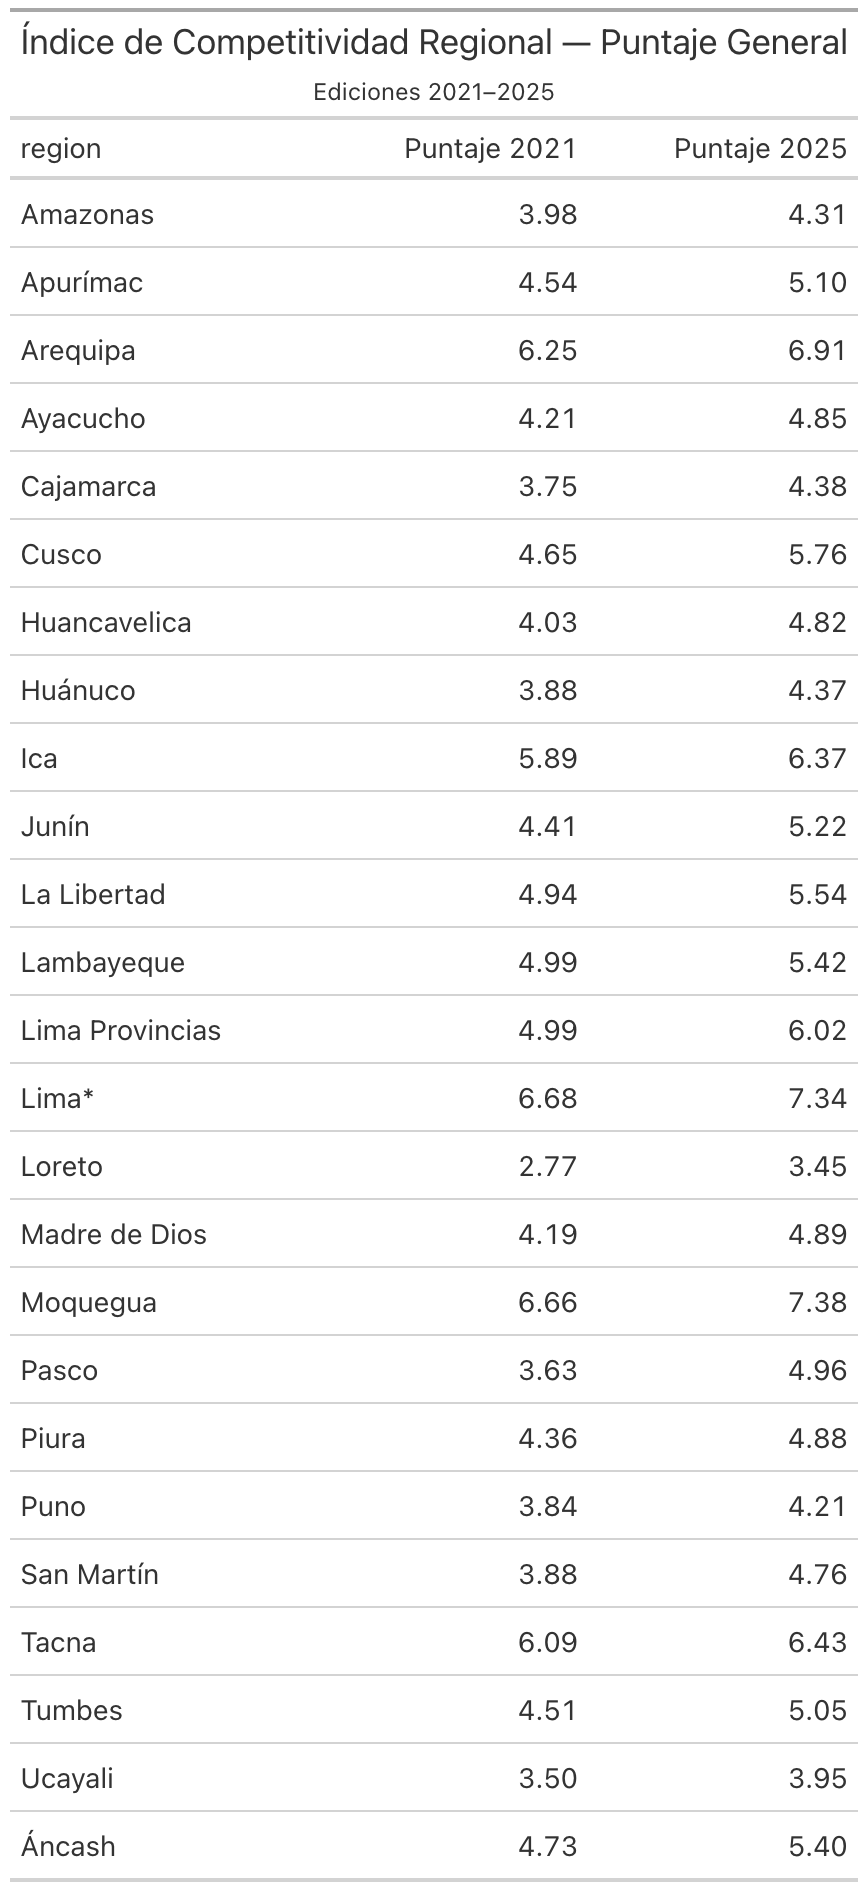
\includegraphics[width=0.9\textwidth,height=\textheight]{tabl1.png}
\end{center}

\textbf{Resultado esperado.} Un objeto gt con título y subtítulo
automáticos, columnas ``Puntaje 2021'' y ``Puntaje 2025'' formateadas a
\textbf{dos decimales}.

\paragraph{\texorpdfstring{\textbf{5) Conjunto mixto (grupo + regiones
explícitas) y salida
gt}}{5) Conjunto mixto (grupo + regiones explícitas) y salida gt}}\label{conjunto-mixto-grupo-regiones-expluxedcitas-y-salida-gt}

\textbf{Se desea lo siguiente:} combinar un \textbf{grupo} y
\textbf{regiones puntuales} en una única tabla de varias ediciones,
lista para reporte.

\begin{Shaded}
\begin{Highlighting}[]
\NormalTok{tab5 }\OtherTok{\textless{}{-}} \FunctionTok{general\_tabla}\NormalTok{(}
  \AttributeTok{ediciones =} \DecValTok{2019}\SpecialCharTok{:}\DecValTok{2025}\NormalTok{,}
  \AttributeTok{regiones  =} \FunctionTok{c}\NormalTok{(}\StringTok{"gr\_sierra"}\NormalTok{, }\StringTok{"Arequipa"}\NormalTok{, }\StringTok{"La Libertad"}\NormalTok{),}
  \AttributeTok{gt        =} \ConstantTok{TRUE}
\NormalTok{)}
\end{Highlighting}
\end{Shaded}

\begin{center}
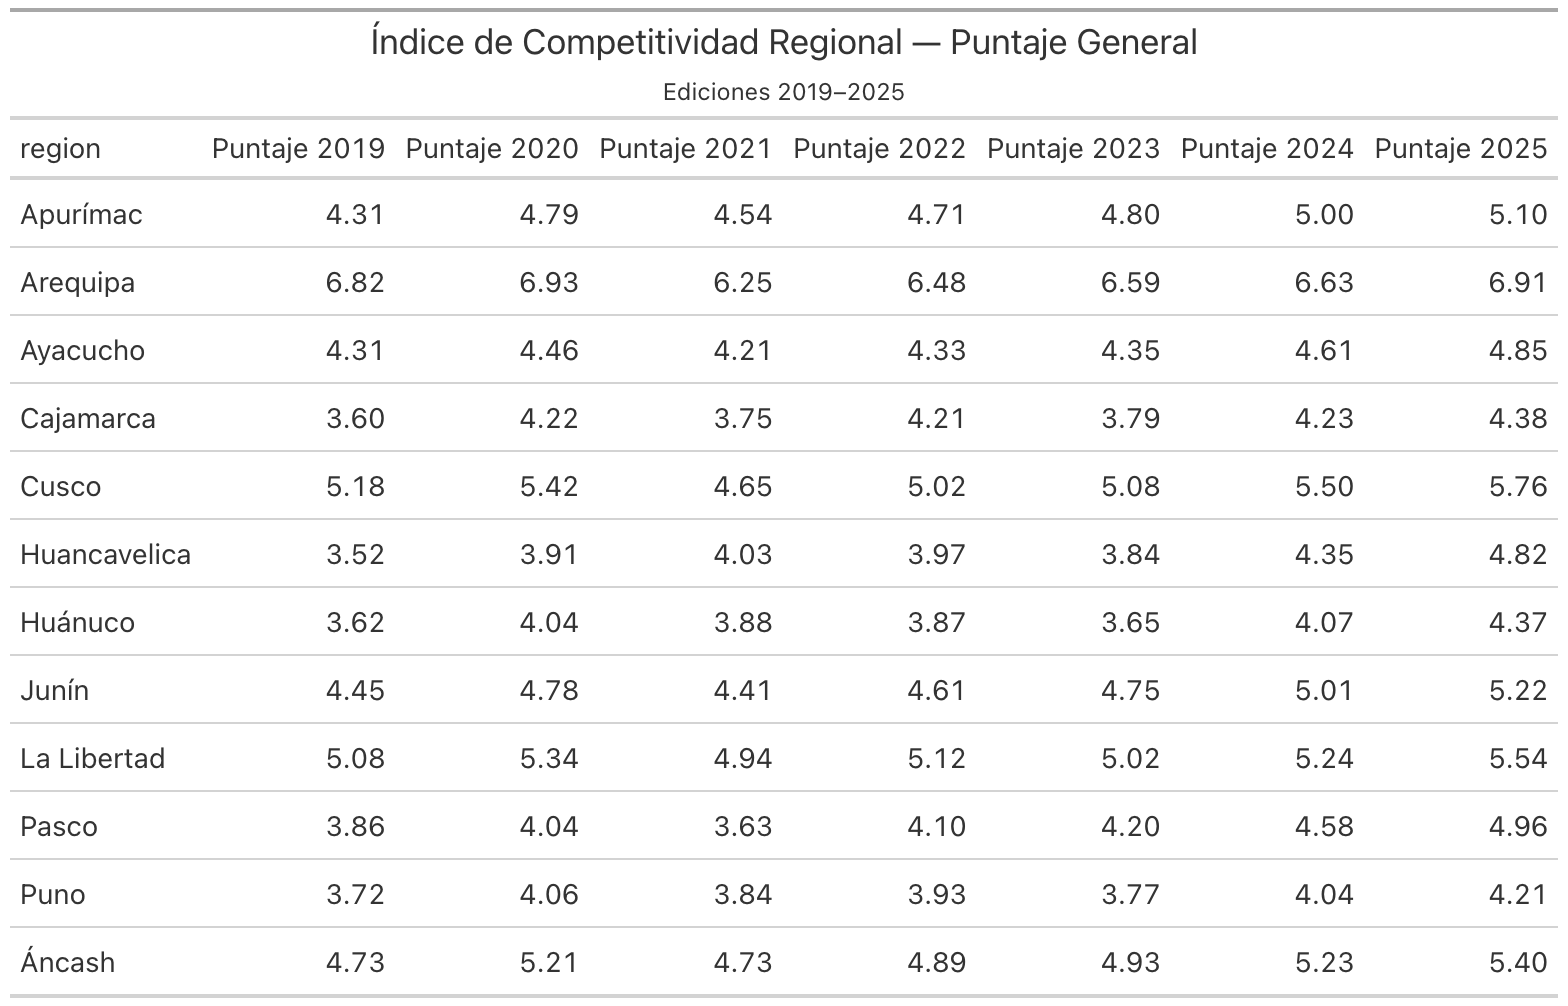
\includegraphics[width=0.9\textwidth,height=\textheight]{obal.png}
\end{center}

\textbf{Resultado esperado.} Una tabla gt con las regiones de gr\_sierra
\textbf{más} Arequipa y La Libertad, y columnas puntaje\_2019 \ldots{}
puntaje\_2025. Lista para exportar o incorporar en un documento.

\subsection{\texorpdfstring{\textbf{general\_barras()}}{general\_barras()}}\label{general_barras}

\textbf{Visualización del puntaje General por región en una edición del
INCORE}

\subsubsection{\texorpdfstring{\textbf{Introducción}}{Introducción}}\label{introducciuxf3n-2}

La función \texttt{general\_barras()} ofrece una representación clara y
jerárquica de los puntajes del \textbf{Índice de Competitividad Regional
(INCORE)} en una edición determinada. Su diseño se centra en el formato
de \textbf{barras horizontales ordenadas de mayor a menor}, lo que
facilita identificar de inmediato las regiones que destacan por su
competitividad y aquellas que se encuentran rezagadas. Esta función
resulta particularmente valiosa cuando se requiere mostrar un panorama
sintético y visualmente contundente del ranking regional, ya sea para
fines académicos, informes de política pública o presentaciones
institucionales.

En el marco del INCORE, donde cada región obtiene un puntaje entre 0 y
10 , la función permite elegir entre dos aproximaciones: representar el
\textbf{índice general total}, que resume el desempeño en los seis
pilares (Entorno Económico, Laboral, Infraestructura, Salud, Educación e
Instituciones), o enfocarse en el \textbf{puntaje General de un pilar
específico}, con lo cual se resalta una dimensión particular de la
competitividad. Esta flexibilidad convierte a general\_barras() en una
herramienta versátil, adecuada tanto para un primer acercamiento como
para análisis más focalizados.

\subsubsection{\texorpdfstring{\textbf{Parámetros}}{Parámetros}}\label{paruxe1metros-1}

La utilización de la función descansa en la combinación de algunos
argumentos clave. Cada uno de ellos abre distintas posibilidades de
análisis:

\begin{itemize}
\item
  \textbf{edicion}: corresponde al año de análisis del INCORE. Debe
  indicarse un valor único dentro del rango de disponibilidad.

  Opciones:

  \begin{itemize}
  \tightlist
  \item
    2016 \ldots{} 2025
  \end{itemize}
\item
  \textbf{pilar}: define si se grafica el índice general total o el
  \textbf{General} de un pilar específico.

  Opciones:

  \begin{itemize}
  \item
    NULL (por defecto: índice general total)
  \item
    ``NOMBRE\_DEL\_PILAR'' (ejemplo: ``Salud'')
  \item
    ``CODIGO\_PILAR'' (ejemplo: ``SAL'')
  \end{itemize}
\item
  \textbf{regiones}: delimita el conjunto de regiones a mostrar. Se
  aceptan nombres, códigos o grupos predefinidos.

  Opciones:

  \begin{itemize}
  \item
    ``ALL'' (por defecto: todas las regiones)
  \item
    c(``REGION1'', ``REGION2'')
  \item
    c(``COD1'', ``COD2'')
  \item
    c(``gr\_norte'', ``gr\_sur'')
  \item
    Combinaciones mixtas (ejemplo: c(``gr\_norte'', ``Lima'', ``La
    Libertad''))
  \end{itemize}
\item
  \textbf{paleta}: establece la paleta cualitativa de colores para
  distinguir regiones.

  Opciones:

  \begin{itemize}
  \item
    ``ipe'' (por defecto, con la gama institucional del paquete)
  \item
    ``okabe\_ito'' (diseñada para accesibilidad visual)
  \item
    ``viridis'' (escala perceptualmente uniforme, útil con muchas
    categorías)
  \end{itemize}
\item
  \textbf{mostrar\_leyenda}: determina si se incluye la leyenda en el
  gráfico.

  Opciones:

  \begin{itemize}
  \item
    FALSE (por defecto)
  \item
    TRUE
  \end{itemize}
\end{itemize}

Los parámetros \textbf{usar\_codigos} e \textbf{incluir\_peru} son
auxiliares: el primero asegura que los códigos regionales o de pilar se
traduzcan a nombres oficiales, mientras que el segundo permite incluir
el promedio nacional de ``Perú'' como referencia en el gráfico.

\subsubsection{\texorpdfstring{\textbf{Explicación
conceptual}}{Explicación conceptual}}\label{explicaciuxf3n-conceptual-1}

El proceso interno de la función puede describirse en tres fases:

\begin{enumerate}
\def\labelenumi{\arabic{enumi}.}
\item
  \textbf{Preparación de datos.} Se leen los resultados del INCORE para
  la edición indicada. Dependiendo de la selección de pilar, se filtra
  el índice general total o el puntaje General de un pilar específico.
\item
  \textbf{Ajustes y filtros.} Se excluye ``Perú'' de manera
  predeterminada (a menos que se indique lo contrario) y se aplica el
  filtro de regiones, con soporte para grupos predefinidos.
  Posteriormente, se consolidan los valores y se asegura que cada región
  tenga un único puntaje.
\item
  \textbf{Visualización.} Se construye un gráfico con barras
  horizontales ordenadas de mayor a menor, etiquetas numéricas con dos
  decimales y una escala fija entre 0 y 10. El uso de colores
  diferenciados por región permite reforzar la legibilidad y la
  comparación.
\end{enumerate}

La salida final es un objeto ggplot, lo que significa que puede ser
modificado, guardado o integrado en flujos de trabajo de visualización
más amplios.

\subsubsection{\texorpdfstring{\textbf{Ejemplos}}{Ejemplos}}\label{ejemplos-1}

\paragraph{\texorpdfstring{\textbf{1) Visualización general de la
edición
2025}}{1) Visualización general de la edición 2025}}\label{visualizaciuxf3n-general-de-la-ediciuxf3n-2025}

\textbf{Se desea lo siguiente:} generar un ranking completo de las 25
regiones para el índice general total en la edición 2025.

\begin{Shaded}
\begin{Highlighting}[]
\NormalTok{graf1 }\OtherTok{\textless{}{-}} \FunctionTok{general\_barras}\NormalTok{(}\AttributeTok{edicion =} \DecValTok{2025}\NormalTok{)}
\NormalTok{graf1}
\end{Highlighting}
\end{Shaded}

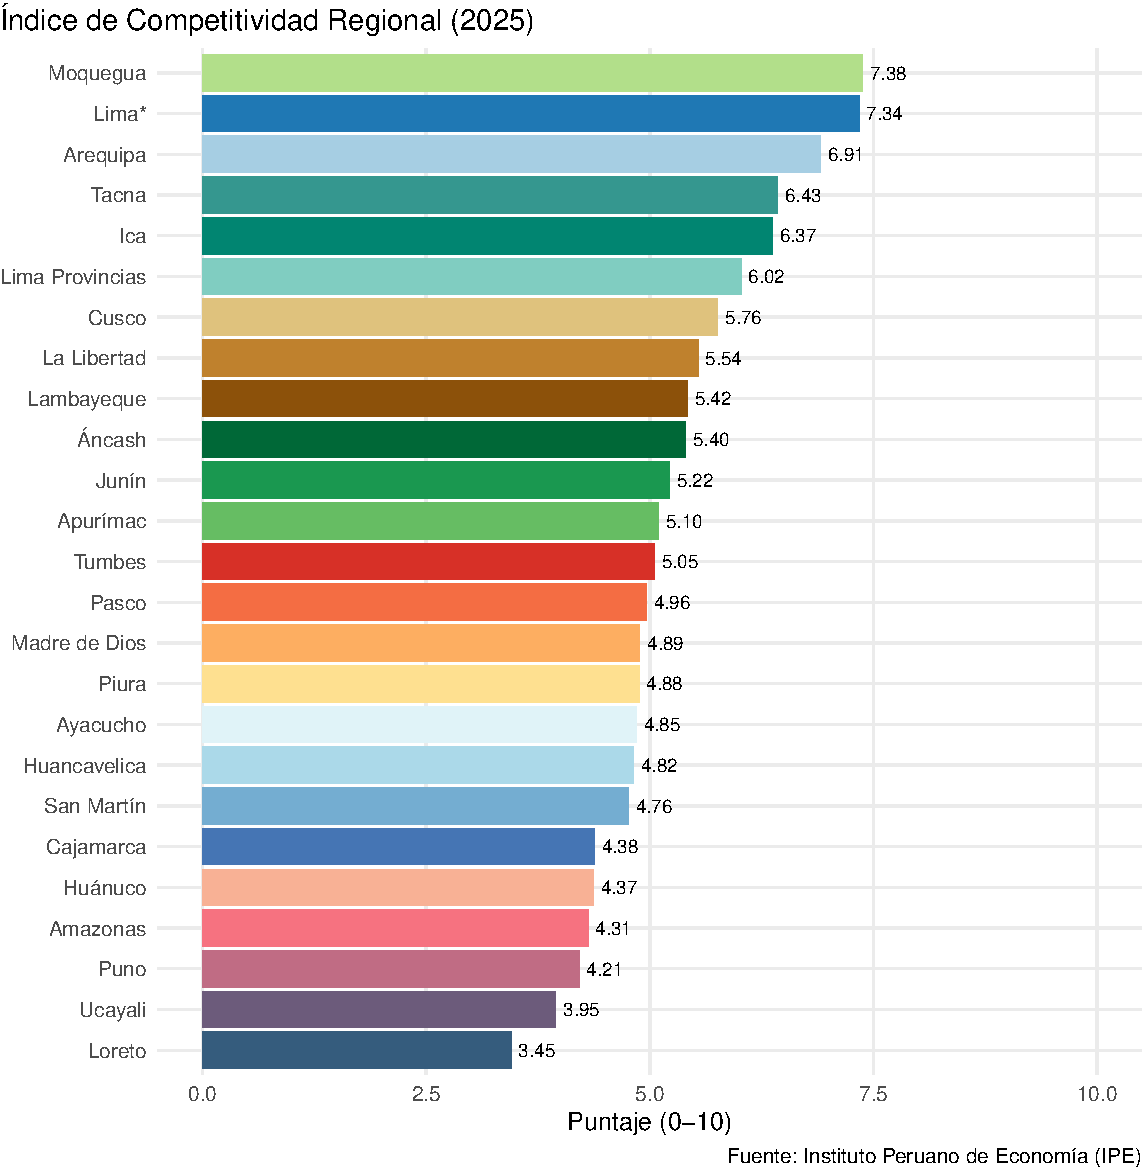
\includegraphics{Manual_files/figure-pdf/unnamed-chunk-16-1.pdf}

\textbf{Resultado esperado.} Un gráfico de barras horizontales que
muestra a todas las regiones ordenadas por su puntaje total en 2025.

\paragraph{\texorpdfstring{\textbf{2) Enfoque por pilar (nombre) con
leyenda
activada}}{2) Enfoque por pilar (nombre) con leyenda activada}}\label{enfoque-por-pilar-nombre-con-leyenda-activada}

\textbf{Se desea lo siguiente:} explorar el desempeño de las regiones en
el pilar de Salud.

\begin{Shaded}
\begin{Highlighting}[]
\NormalTok{graf2 }\OtherTok{\textless{}{-}} \FunctionTok{general\_barras}\NormalTok{(}
  \AttributeTok{edicion =} \DecValTok{2025}\NormalTok{,}
  \AttributeTok{pilar =} \StringTok{"Salud"}\NormalTok{,}
  \AttributeTok{mostrar\_leyenda =} \ConstantTok{TRUE}
\NormalTok{)}
\NormalTok{graf2}
\end{Highlighting}
\end{Shaded}

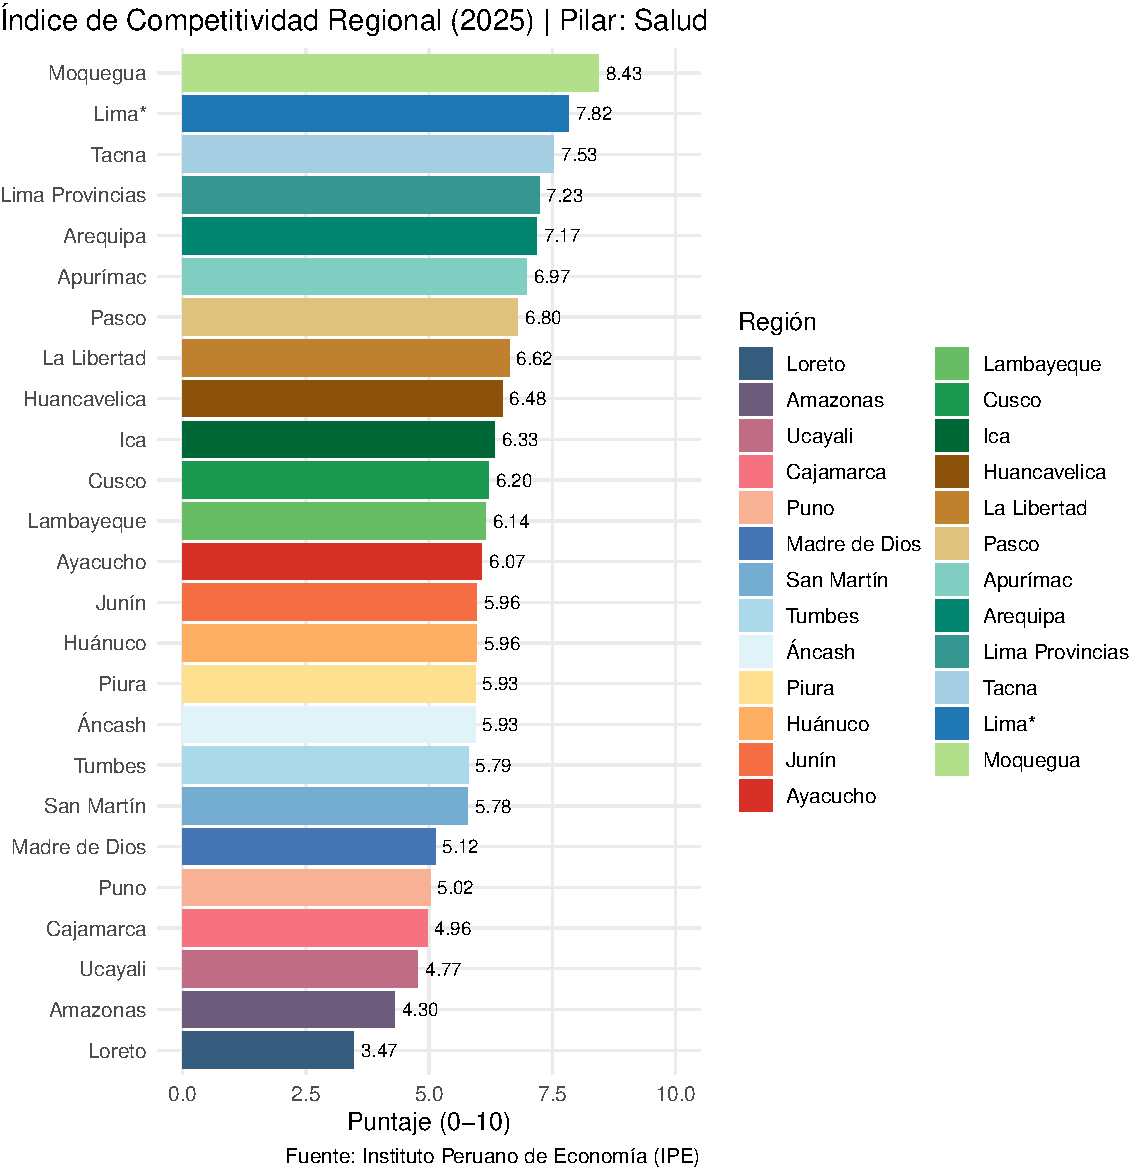
\includegraphics{Manual_files/figure-pdf/unnamed-chunk-17-1.pdf}

\textbf{Resultado esperado.} Ranking regional para el pilar Salud, con
la leyenda activada para identificar los colores asociados.

\paragraph{\texorpdfstring{\textbf{3) Subconjunto de regiones (grupo y
nombres)}}{3) Subconjunto de regiones (grupo y nombres)}}\label{subconjunto-de-regiones-grupo-y-nombres}

\textbf{Se desea lo siguiente:} reducir la visualización a un grupo de
regiones del norte y dos regiones adicionales.

\begin{Shaded}
\begin{Highlighting}[]
\NormalTok{graf3 }\OtherTok{\textless{}{-}} \FunctionTok{general\_barras}\NormalTok{(}
  \AttributeTok{edicion =} \DecValTok{2025}\NormalTok{,}
  \AttributeTok{regiones =} \FunctionTok{c}\NormalTok{(}\StringTok{"gr\_norte"}\NormalTok{, }\StringTok{"Lima*"}\NormalTok{, }\StringTok{"La Libertad"}\NormalTok{)}
\NormalTok{)}
\NormalTok{graf3}
\end{Highlighting}
\end{Shaded}

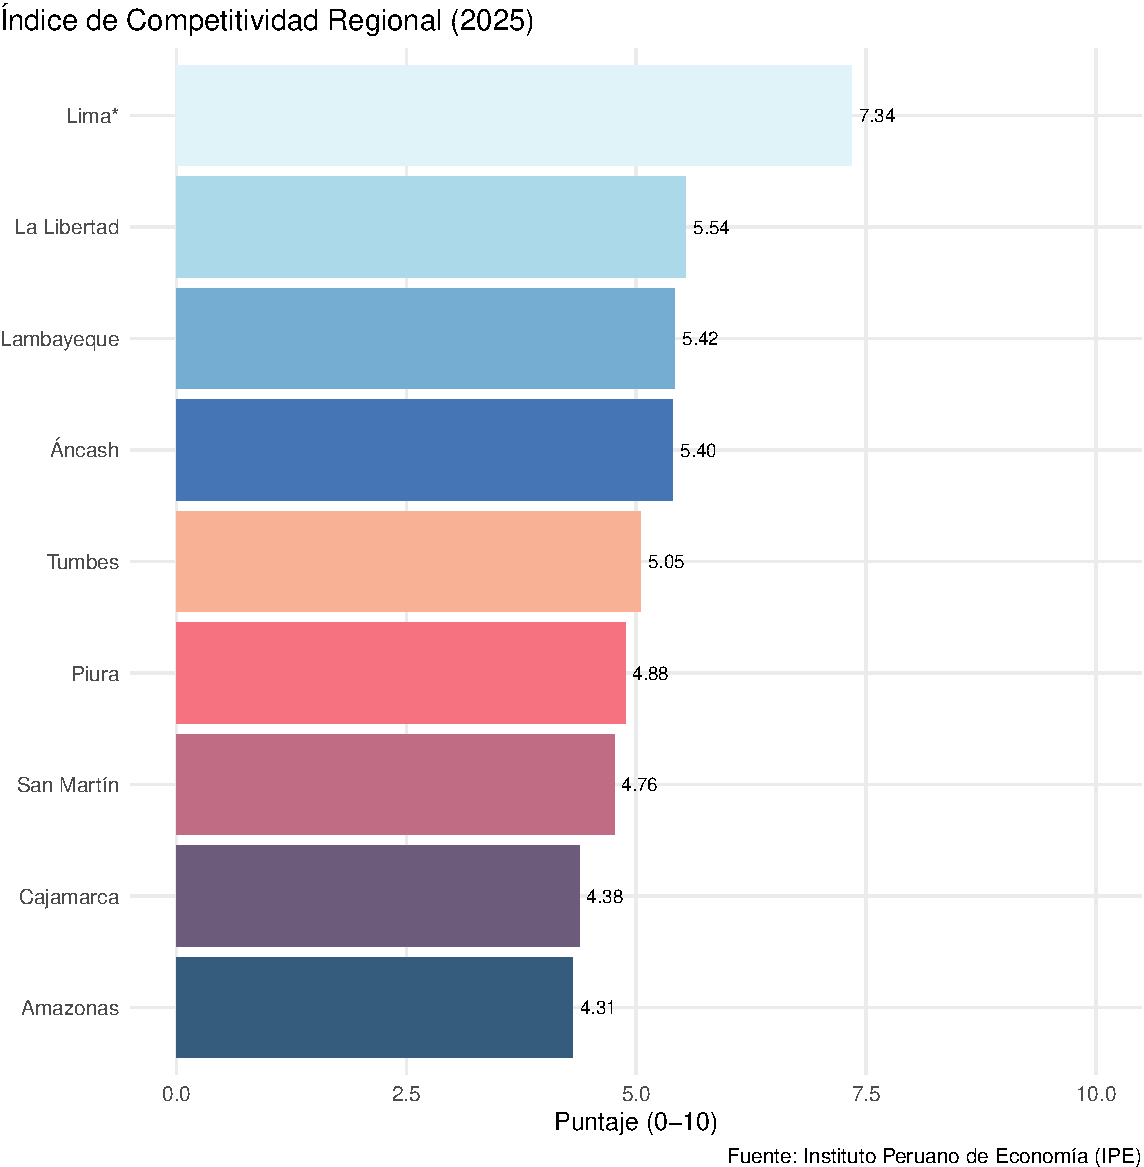
\includegraphics{Manual_files/figure-pdf/unnamed-chunk-18-1.pdf}

\textbf{Resultado esperado.} Un gráfico con solo las regiones
especificadas, manteniendo la escala común de 0 a 10.

\paragraph{\texorpdfstring{\textbf{4) Inclusión de ``Perú'' y cambio de
paleta}}{4) Inclusión de ``Perú'' y cambio de paleta}}\label{inclusiuxf3n-de-peruxfa-y-cambio-de-paleta}

\textbf{Se desea lo siguiente:} incluir la referencia nacional y
utilizar una paleta perceptualmente uniforme.

\begin{Shaded}
\begin{Highlighting}[]
\NormalTok{graf4 }\OtherTok{\textless{}{-}} \FunctionTok{general\_barras}\NormalTok{(}
  \AttributeTok{edicion =} \DecValTok{2025}\NormalTok{,}
  \AttributeTok{pilar =} \StringTok{"Infraestructura"}\NormalTok{,}
  \AttributeTok{incluir\_peru =} \ConstantTok{TRUE}\NormalTok{,}
  \AttributeTok{paleta =} \StringTok{"viridis"}
\NormalTok{)}
\NormalTok{graf4}
\end{Highlighting}
\end{Shaded}

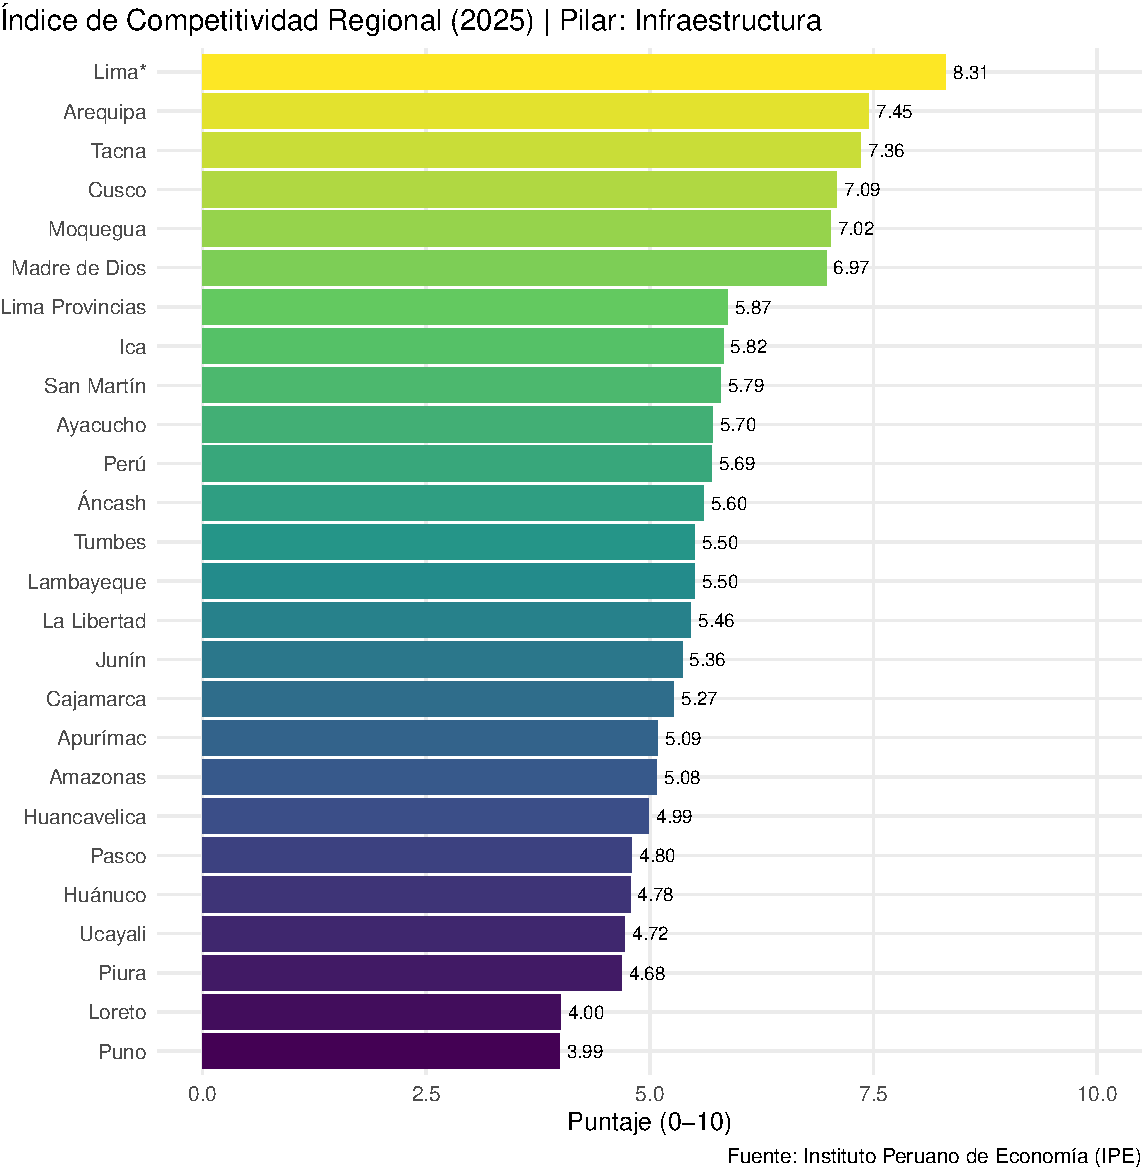
\includegraphics{Manual_files/figure-pdf/unnamed-chunk-19-1.pdf}

\textbf{Resultado esperado.} Ranking del pilar Infraestructura con la
fila ``Perú'' como punto de comparación y colores adaptados a
``viridis''.

\paragraph{\texorpdfstring{\textbf{5) Comparación focalizada de regiones
líderes y
rezagadas}}{5) Comparación focalizada de regiones líderes y rezagadas}}\label{comparaciuxf3n-focalizada-de-regiones-luxedderes-y-rezagadas}

\textbf{Se desea lo siguiente:} destacar únicamente sesis regiones del
índice general total en 2025.

\begin{Shaded}
\begin{Highlighting}[]
\NormalTok{graf5 }\OtherTok{\textless{}{-}} \FunctionTok{general\_barras}\NormalTok{(}
  \AttributeTok{edicion =} \DecValTok{2025}\NormalTok{,}
  \AttributeTok{regiones =} \FunctionTok{c}\NormalTok{(}\StringTok{"Moquegua"}\NormalTok{, }\StringTok{"Lima*"}\NormalTok{, }\StringTok{"Arequipa"}\NormalTok{,}
               \StringTok{"Loreto"}\NormalTok{, }\StringTok{"Ucayali"}\NormalTok{, }\StringTok{"Puno"}\NormalTok{),}
  \AttributeTok{paleta =} \StringTok{"okabe\_ito"}\NormalTok{,}
  \AttributeTok{mostrar\_leyenda =} \ConstantTok{TRUE}
\NormalTok{)}
\NormalTok{graf5}
\end{Highlighting}
\end{Shaded}

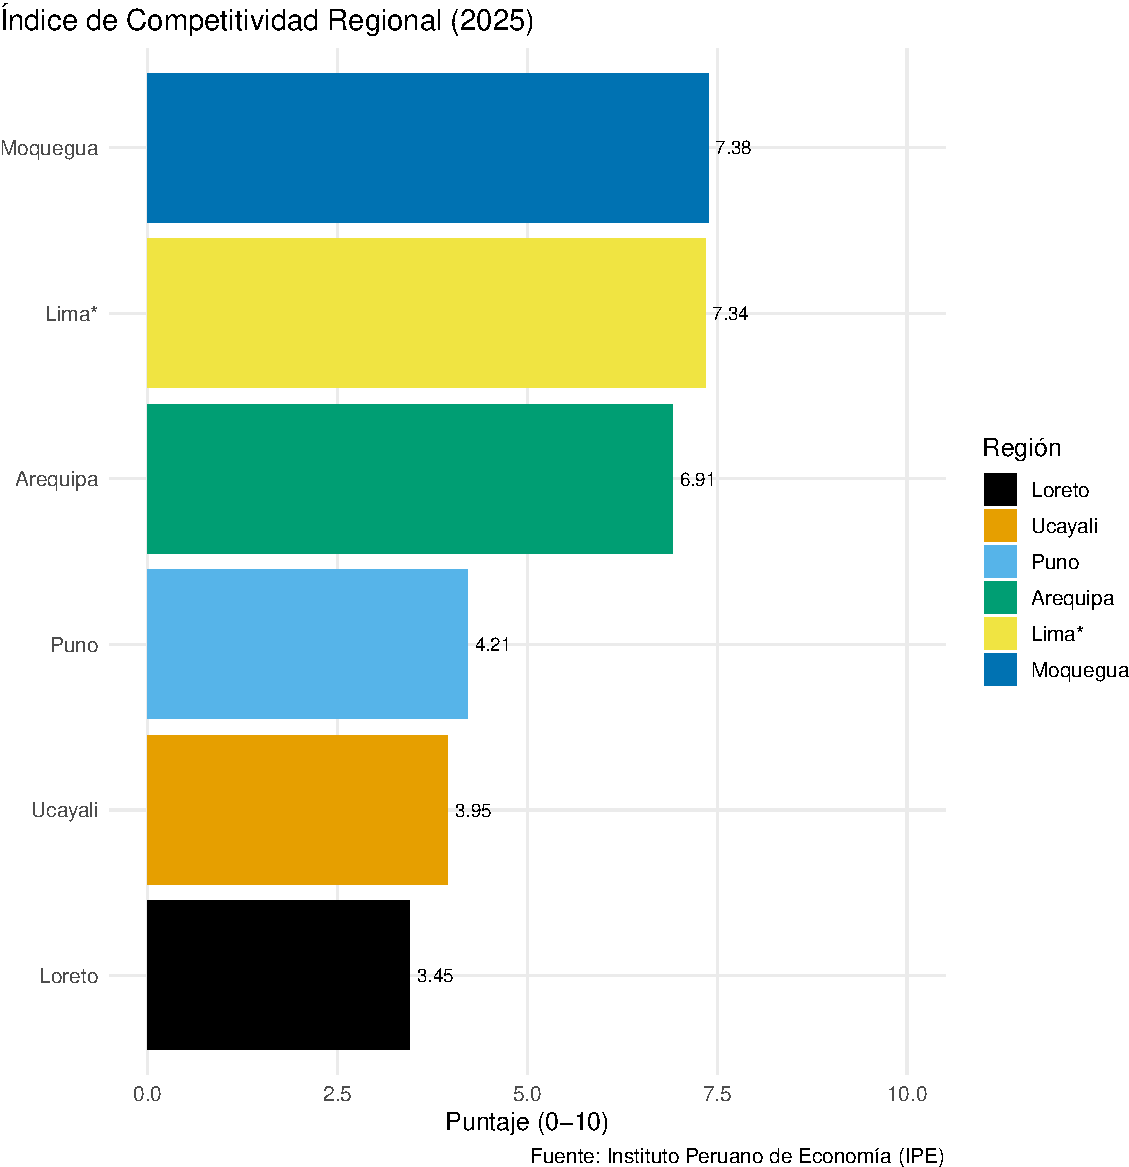
\includegraphics{Manual_files/figure-pdf/unnamed-chunk-20-1.pdf}

\textbf{Resultado esperado.} Gráfico con seis barras que permiten
comparar visualmente el contraste entre los primeros lugares (Moquegua,
Lima*, Arequipa) y los últimos (Loreto, Ucayali, Puno), siguiendo los
resultados oficiales del INCORE .

\subsection{\texorpdfstring{\textbf{general\_dispersion\_pilares()}}{general\_dispersion\_pilares()}}\label{general_dispersion_pilares}

\textbf{Dispersión del puntaje General por pilar (una edición)}

La función integra la familia de visualizaciones general\_* y su
objetivo es representar, para una \textbf{edición} del INCORE, la
\textbf{distribución del puntaje General (0--10)} de las regiones
\textbf{a lo largo de los pilares}. Cada \textbf{pilar} constituye el
eje \textbf{X} y cada \textbf{punto} corresponde al puntaje
\textbf{General} de una \textbf{región} en ese pilar. El resultado es
una vista \textbf{comparativa y transversal}: permite observar, en un
mismo gráfico, cómo se ``abren'' o ``cierran'' las dispersiones por
pilar, dónde se ubica el \textbf{promedio nacional} y qué tan
heterogéneo es el desempeño por dimensión.

\subsubsection{\texorpdfstring{\textbf{Introducción}}{Introducción}}\label{introducciuxf3n-3}

general\_dispersion\_pilares() aborda un problema típico en informes
comparativos: \textbf{entender la variabilidad entre regiones por
dimensiones} (pilares) dentro de un mismo año. Mientras que un ranking
de barras prioriza el orden, esta función prioriza la
\textbf{distribución}: ¿en qué pilares existe mayor concentración de
regiones en torno a valores similares? ¿Dónde se observan colas más
pronunciadas? ¿Cómo se ubican las regiones respecto del \textbf{promedio
nacional}? La lectura simultánea por pilares facilita detectar
\textbf{asimetrías}: por ejemplo, un pilar con medias similares pero
\textbf{dispersión alta} frente a otro con \textbf{dispersión baja}, o
clusters de regiones que tienden a agruparse en determinados pilares.

\subsubsection{\texorpdfstring{\textbf{Parámetros}}{Parámetros}}\label{paruxe1metros-2}

La lógica de uso parte de una \textbf{edición} y, opcionalmente, filtros
de \textbf{regiones} y \textbf{pilares}. Existen además parámetros de
\textbf{estética} que permiten aclarar la lectura (jitter para separar
puntos, estilo del promedio) y una \textbf{paleta cualitativa} para
distinguir regiones.

\begin{itemize}
\item
  \textbf{edicion}: fija la \textbf{edición (año)} del INCORE a
  visualizar.

  Opciones y formato:

  \begin{itemize}
  \item
    integer(1)
  \item
    2016 \ldots{} 2025
  \end{itemize}
\item
  \textbf{regiones}: delimita el \textbf{universo de regiones} a
  mostrar, admite nombres, códigos, \textbf{grupos gr\_*}, e
  \textbf{inclusiones/exclusiones} con prefijos como ``-''.

  Opciones y formato:

  \begin{itemize}
  \item
    ``ALL'' (por defecto: todas las regiones)
  \item
    c(``REGION1'', ``REGION2'')
  \item
    c(``COD1'', ``COD2'')
  \item
    c(``gr\_costa'', ``gr\_sierra'', ``gr\_selva'') (según los grupos
    definidos en el paquete)
  \item
    Exclusiones: ``-Lima*'' (ejemplo de patrón para excluir)
  \item
    Combinaciones mixtas: c(``gr\_costa'', ``La Libertad'', ``-Lima*'')
  \end{itemize}
\item
  \textbf{pilares}: selecciona los \textbf{pilares} a incluir, puede
  mezclar \textbf{nombres} y \textbf{códigos} (si se cuenta con
  catálogos activos).

  Opciones y formato:

  \begin{itemize}
  \item
    ``ALL'' (por defecto: ``Entorno económico'', ``Laboral'',
    ``Infraestructura'', ``Salud'', ``Educación'', ``Instituciones'')
  \item
    Nombres: c(``Salud'', ``Educación'')
  \item
    Códigos: c(``SAL'', ``EDU'')
  \item
    Mezcla: c(``SAL'', ``Educación'', ``INF'')
  \end{itemize}
\item
  \textbf{paleta}: paleta \textbf{cualitativa} para colorear \textbf{por
  región} (colores consistentes a través de pilares).

  Opciones y formato:

  \begin{itemize}
  \item
    ``ipe'' (por defecto)
  \item
    ``okabe\_ito'' (accesible para daltonismo)
  \item
    ``viridis'' (perceptualmente uniforme, recomendable con muchas
    regiones)
  \end{itemize}
\item
  \textbf{mostrar\_promedio}: añade un \textbf{marcador del promedio
  nacional} (promedio entre regiones) por \textbf{pilar}.

  Opciones y formato:

  \begin{itemize}
  \item
    TRUE (por defecto)
  \item
    FALSE
  \end{itemize}
\item
  \textbf{promedio\_shape}, \textbf{promedio\_size},
  \textbf{promedio\_color}, \textbf{promedio\_fill}: controlan la
  \textbf{estética} del marcador de promedio (forma, tamaño, color de
  borde y relleno).

  Opciones (típicas):

  \begin{itemize}
  \item
    promedio\_shape = 23 (rombo relleno)
  \item
    promedio\_size = 3.5
  \item
    promedio\_color = ``black''
  \item
    promedio\_fill = ``white''
  \end{itemize}
\item
  \textbf{jitter\_width}, \textbf{jitter\_height}: amplitud del
  \textbf{jitter} para \textbf{separar} puntos que podrían superponerse
  vertical u horizontalmente.

  Opciones y formato:

  \begin{itemize}
  \item
    jitter\_width = 0.08 (por defecto)
  \item
    jitter\_height = 0.0 (por defecto)
  \end{itemize}
\end{itemize}

El parámetro \textbf{usar\_codigos} cumple una función operativa
secundaria: si es TRUE, habilita la \textbf{traducción} de códigos de
región/pilar a nombres oficiales mediante los catálogos del paquete,
manteniendo consistencia editorial.

\subsubsection{\texorpdfstring{\textbf{Explicación
conceptual}}{Explicación conceptual}}\label{explicaciuxf3n-conceptual-2}

La función \textbf{lee} los datos de la edición indicada,
\textbf{filtra} las filas correspondientes al \textbf{indicador
``General''} de cada \textbf{pilar canónico} y \textbf{excluye} la fila
``Perú'' para concentrar el análisis en dispersiones
\textbf{inter-regionales}. Si se especifican pilares, traduce y filtra
según nombres/códigos, si se especifican regiones, resuelve
\textbf{grupos gr\_*} y \textbf{exclusiones}. Como salvaguarda,
\textbf{consolida} un valor por (región, pilar) y prepara una
\textbf{paleta} cualitativa estable para todas las regiones del
subconjunto. La marcación del \textbf{promedio nacional} añade un
\textbf{referente} en cada pilar, útil para identificar pilares por
encima/por debajo de la media. La geometría base es un
\textbf{geom\_jitter} con límites fijos \textbf{0--10} en y, lo que
estandariza la comparación entre pilares y evita interpretaciones
sensibles a escalas variables.

\subsubsection{\texorpdfstring{\textbf{Ejemplos}}{Ejemplos}}\label{ejemplos-2}

\paragraph{\texorpdfstring{\textbf{1) Dispersión completa por pilares en
una
edición}}{1) Dispersión completa por pilares en una edición}}\label{dispersiuxf3n-completa-por-pilares-en-una-ediciuxf3n}

\textbf{Se desea lo siguiente:} visualizar la dispersión del
\textbf{puntaje General} de todas las regiones en \textbf{todos los
pilares} para una edición reciente.

\begin{Shaded}
\begin{Highlighting}[]
\NormalTok{p1 }\OtherTok{\textless{}{-}} \FunctionTok{general\_dispersion\_pilares}\NormalTok{(}
  \AttributeTok{edicion =} \DecValTok{2025}\NormalTok{,}
  \AttributeTok{regiones =} \StringTok{"ALL"}\NormalTok{,}
  \AttributeTok{pilares  =} \StringTok{"ALL"}
\NormalTok{)}
\NormalTok{p1}
\end{Highlighting}
\end{Shaded}

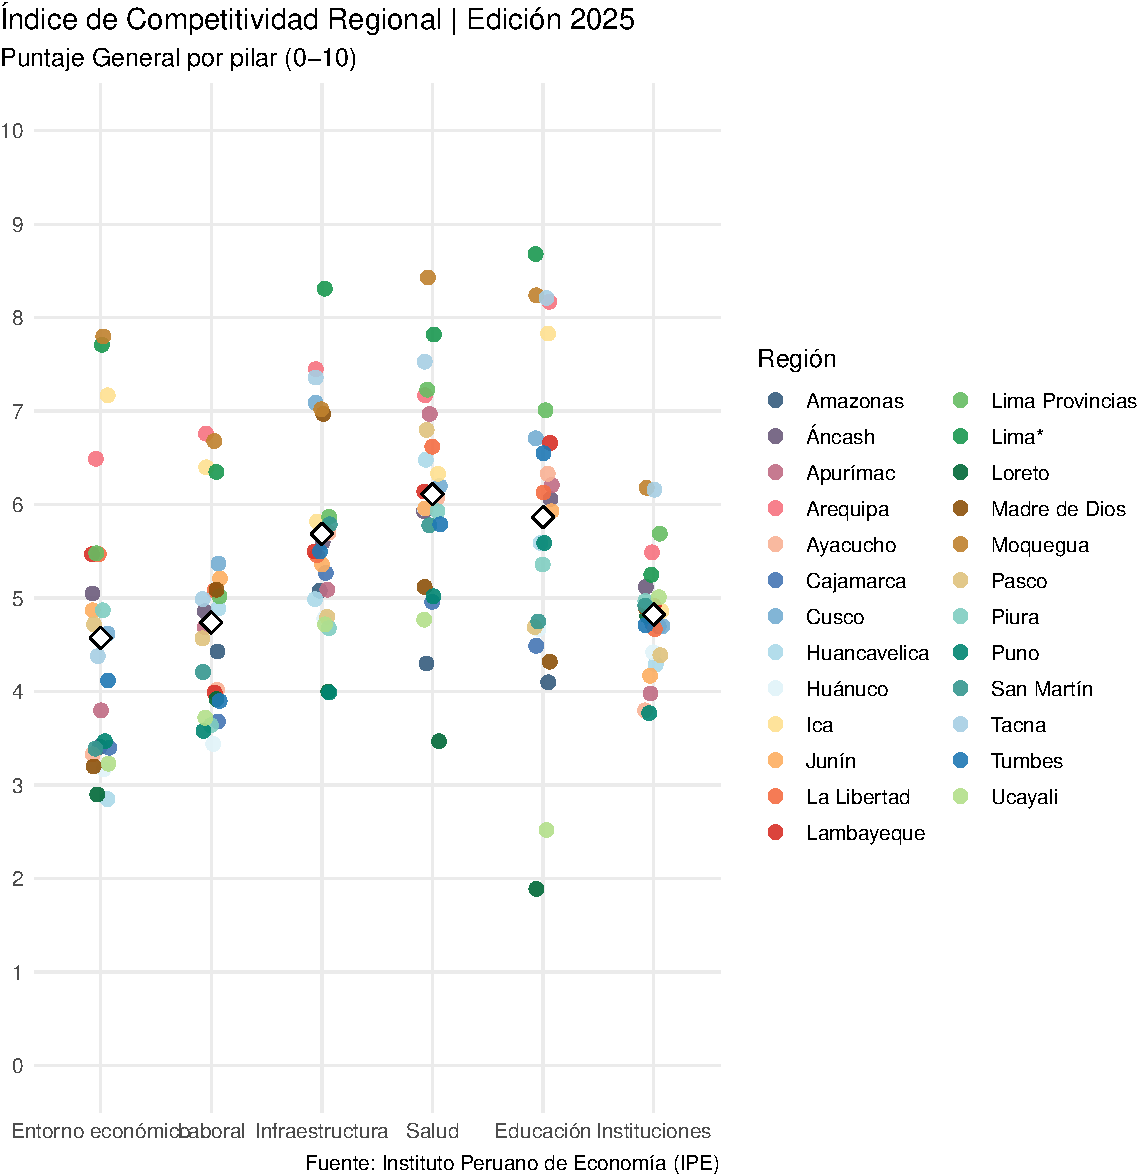
\includegraphics{Manual_files/figure-pdf/unnamed-chunk-21-1.pdf}

\textbf{Resultado esperado.} Puntos por región en cada pilar, con
\textbf{promedio nacional} marcado (por defecto). Permite detectar
pilares con \textbf{dispersión alta/baja} y la posición de la media en
cada uno.

\paragraph{\texorpdfstring{\textbf{2) Subconjunto territorial con grupos
y
exclusiones}}{2) Subconjunto territorial con grupos y exclusiones}}\label{subconjunto-territorial-con-grupos-y-exclusiones}

\textbf{Se desea lo siguiente:} revisar la dispersión solo para
\textbf{costa} y excluir \textbf{Lima}* para observar la estructura sin
el mayor outlier urbano.

\begin{Shaded}
\begin{Highlighting}[]
\NormalTok{p2 }\OtherTok{\textless{}{-}} \FunctionTok{general\_dispersion\_pilares}\NormalTok{(}
  \AttributeTok{edicion =} \DecValTok{2025}\NormalTok{,}
  \AttributeTok{regiones =} \FunctionTok{c}\NormalTok{(}\StringTok{"gr\_costa"}\NormalTok{, }\StringTok{"{-}Lima*"}\NormalTok{),}
  \AttributeTok{pilares  =} \StringTok{"ALL"}\NormalTok{,}
  \AttributeTok{paleta   =} \StringTok{"okabe\_ito"}
\NormalTok{)}
\NormalTok{p2}
\end{Highlighting}
\end{Shaded}

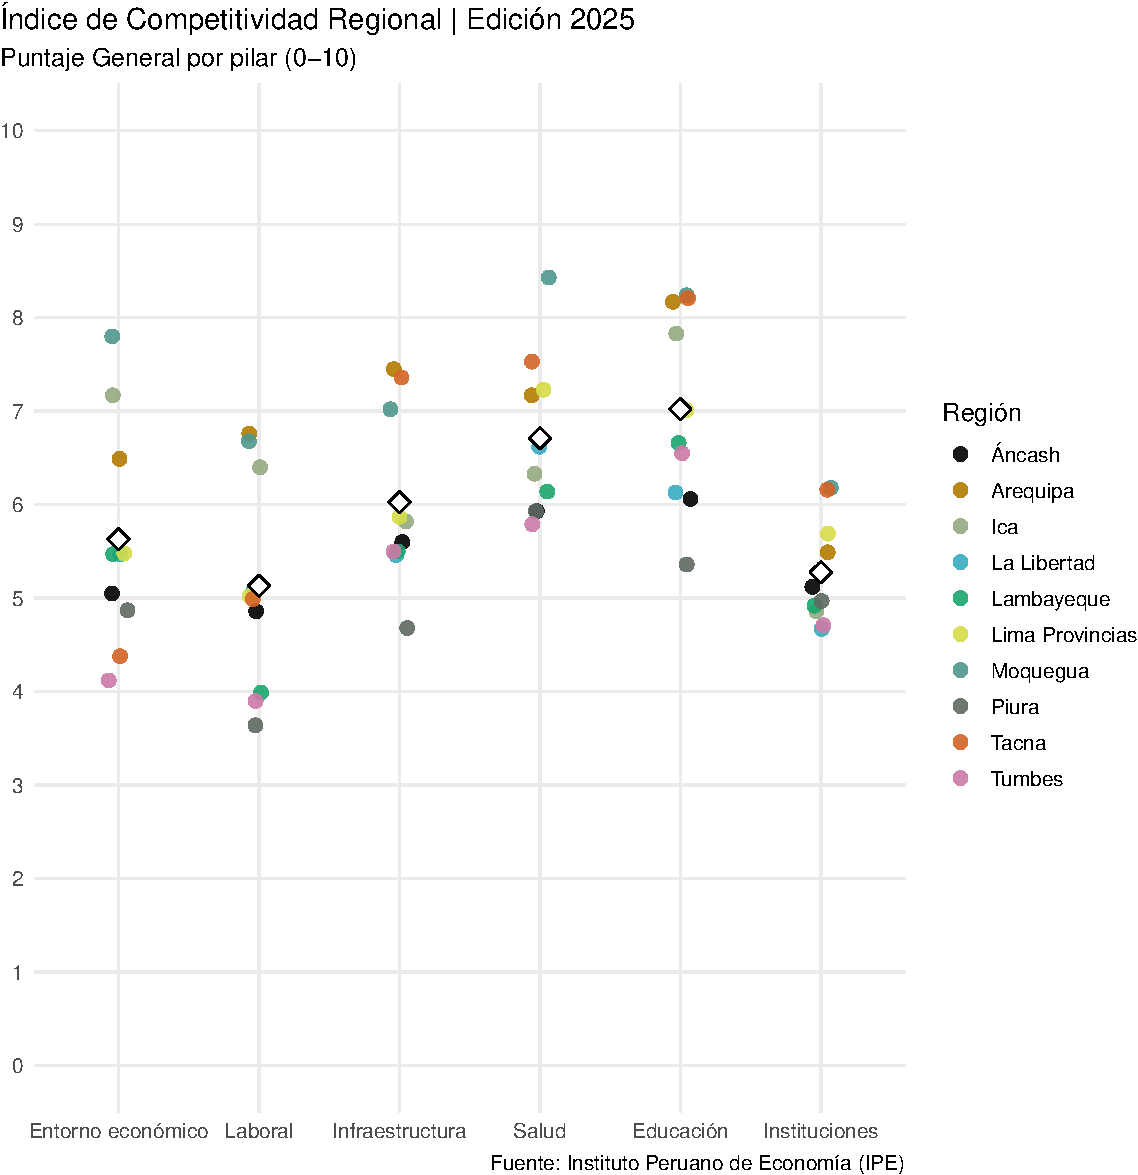
\includegraphics{Manual_files/figure-pdf/unnamed-chunk-22-1.pdf}

\textbf{Resultado esperado.} Dispersión enfocada en la \textbf{costa}
sin Lima*, coloreada con una paleta accesible para daltonismo. La
comparación por pilar revela si, sin Lima*, cambian los pilares con
mayor/menor heterogeneidad.

\paragraph{\texorpdfstring{\textbf{3) Selección de pilares por
código}}{3) Selección de pilares por código}}\label{selecciuxf3n-de-pilares-por-cuxf3digo}

\textbf{Se desea lo siguiente:} comparar únicamente \textbf{Salud} e
\textbf{Infraestructura} utilizando códigos, manteniendo el promedio
visible.

\begin{Shaded}
\begin{Highlighting}[]
\NormalTok{p3 }\OtherTok{\textless{}{-}} \FunctionTok{general\_dispersion\_pilares}\NormalTok{(}
  \AttributeTok{edicion =} \DecValTok{2025}\NormalTok{,}
  \AttributeTok{regiones =} \StringTok{"ALL"}\NormalTok{,}
  \AttributeTok{pilares  =} \FunctionTok{c}\NormalTok{(}\StringTok{"SAL"}\NormalTok{, }\StringTok{"INF"}\NormalTok{),}
  \AttributeTok{mostrar\_promedio =} \ConstantTok{TRUE}
\NormalTok{)}
\NormalTok{p3}
\end{Highlighting}
\end{Shaded}

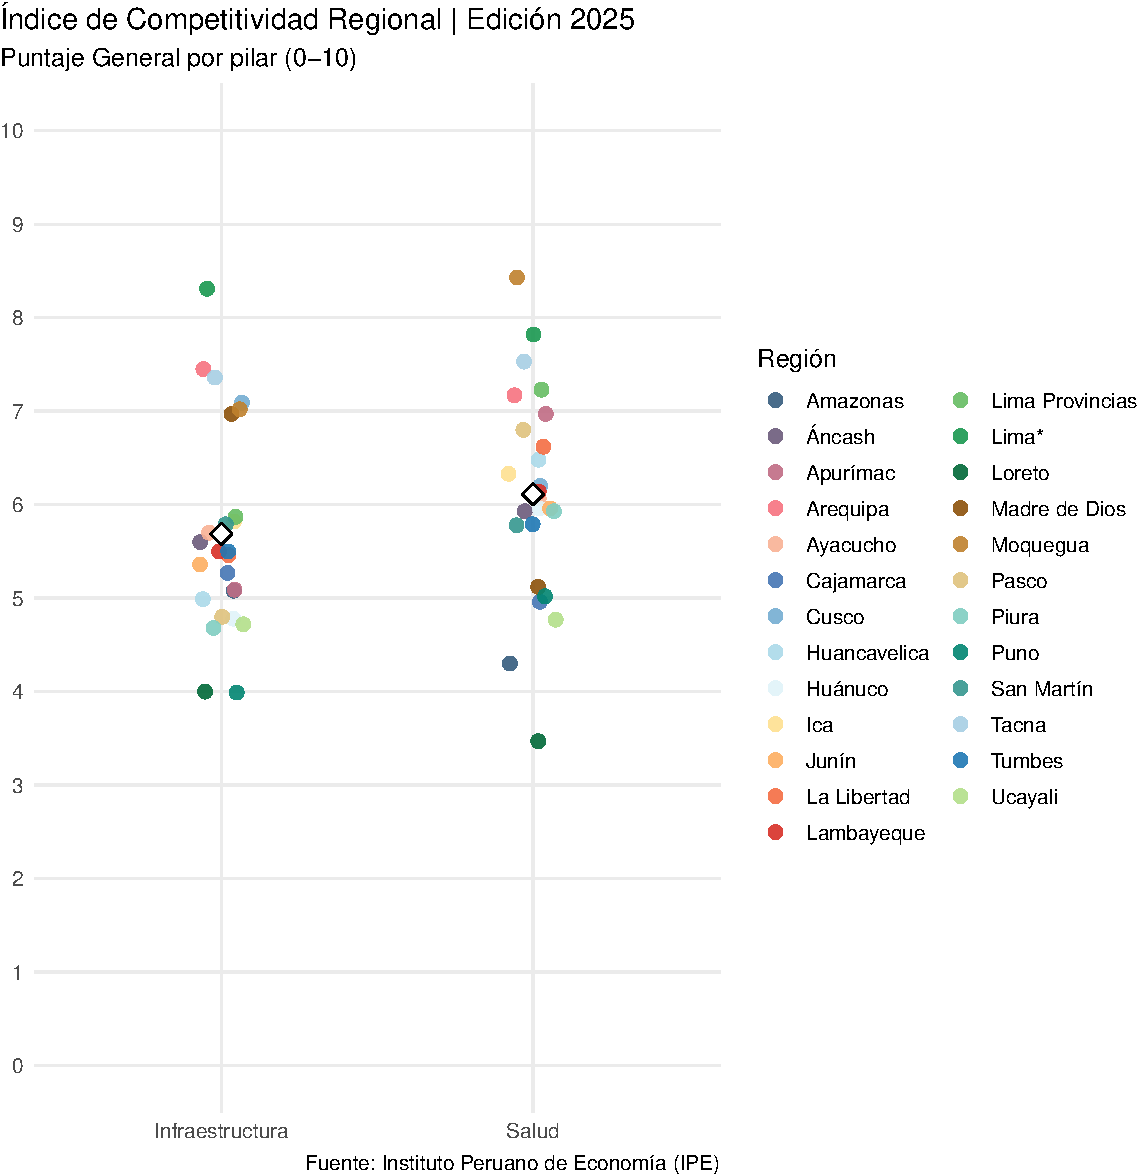
\includegraphics{Manual_files/figure-pdf/unnamed-chunk-23-1.pdf}

\textbf{Resultado esperado.} Dispersión centrada en \textbf{dos pilares}
clave, el \textbf{promedio nacional} por pilar facilita contrastar si la
mediana subjetiva de los puntos coincide o no con la media trazada.

\paragraph{\texorpdfstring{\textbf{4) Lectura fina en un bloque mixto de
regiones}}{4) Lectura fina en un bloque mixto de regiones}}\label{lectura-fina-en-un-bloque-mixto-de-regiones}

\textbf{Se desea lo siguiente:} inspeccionar un \textbf{bloque mixto}
(grupo + regiones puntuales) y ajustar el \textbf{jitter} para separar
puntos muy cercanos.

\begin{Shaded}
\begin{Highlighting}[]
\NormalTok{p4 }\OtherTok{\textless{}{-}} \FunctionTok{general\_dispersion\_pilares}\NormalTok{(}
  \AttributeTok{edicion =} \DecValTok{2025}\NormalTok{,}
  \AttributeTok{regiones =} \FunctionTok{c}\NormalTok{(}\StringTok{"gr\_costa"}\NormalTok{, }\StringTok{"Cusco"}\NormalTok{, }\StringTok{"Arequipa"}\NormalTok{),}
  \AttributeTok{pilares  =} \FunctionTok{c}\NormalTok{(}\StringTok{"Educación"}\NormalTok{, }\StringTok{"Instituciones"}\NormalTok{, }\StringTok{"Laboral"}\NormalTok{),}
  \AttributeTok{jitter\_width  =} \FloatTok{0.12}\NormalTok{,}
  \AttributeTok{jitter\_height =} \FloatTok{0.02}\NormalTok{,}
  \AttributeTok{paleta =} \StringTok{"viridis"}
\NormalTok{)}
\NormalTok{p4}
\end{Highlighting}
\end{Shaded}

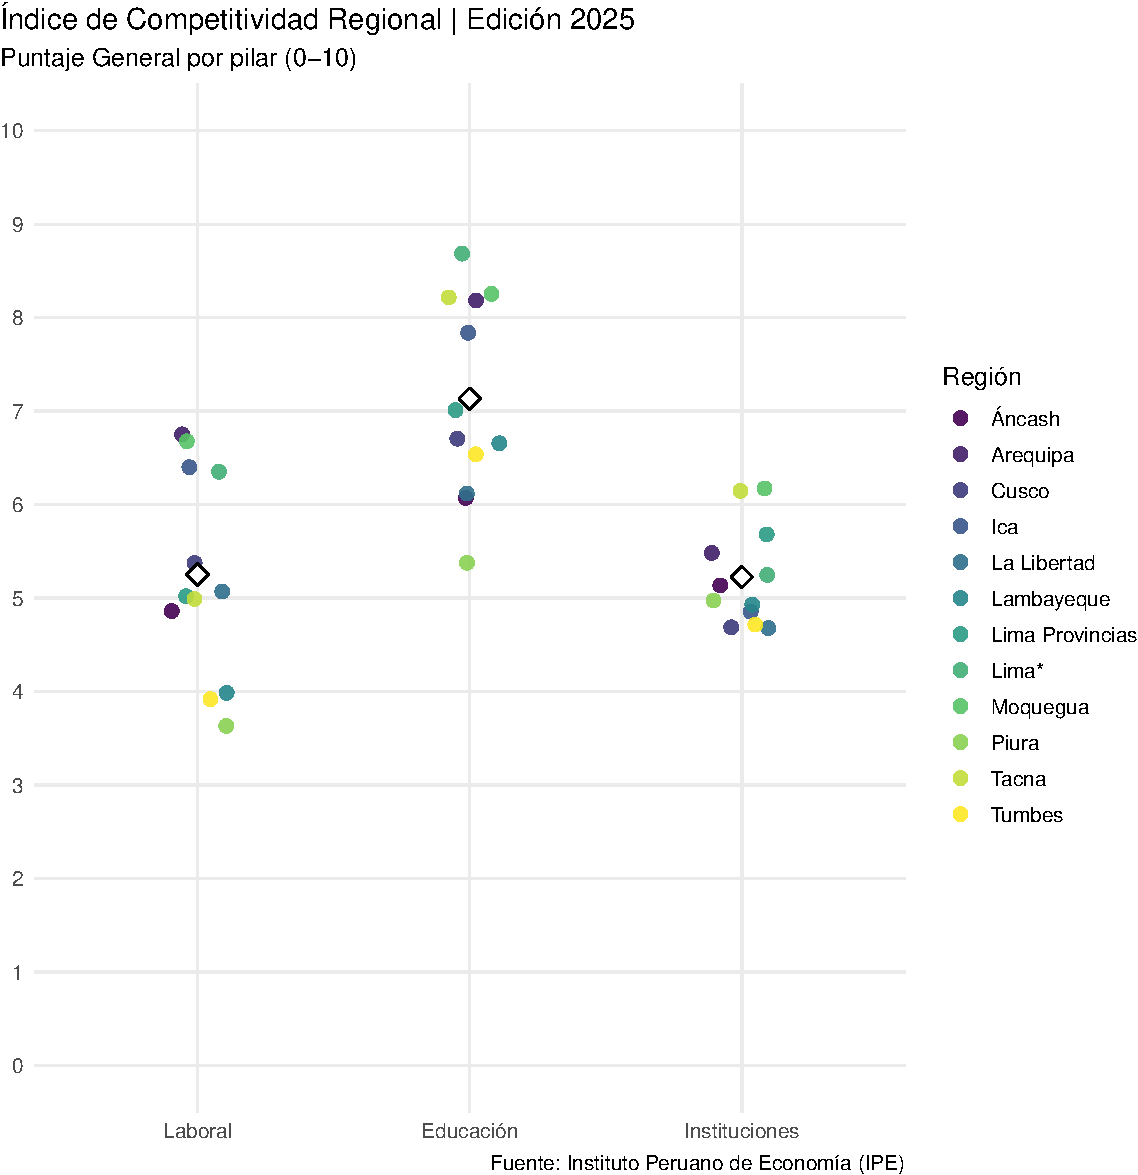
\includegraphics{Manual_files/figure-pdf/unnamed-chunk-24-1.pdf}

\textbf{Resultado esperado.} Mejor separación visual de puntos
\textbf{muy próximos} dentro de los pilares seleccionados, la paleta
``viridis'' mantiene distinguibilidad cuando hay varias regiones en un
mismo rango.

\paragraph{\texorpdfstring{\textbf{5) Vista focal con mezcla de
nombres/códigos y promedio
estilizado}}{5) Vista focal con mezcla de nombres/códigos y promedio estilizado}}\label{vista-focal-con-mezcla-de-nombrescuxf3digos-y-promedio-estilizado}

\textbf{Se desea lo siguiente:} centrar la lectura en \textbf{tres
pilares} combinando nombres y códigos, con un \textbf{promedio} más
visible por forma/tamaño.

\begin{Shaded}
\begin{Highlighting}[]
\NormalTok{p5 }\OtherTok{\textless{}{-}} \FunctionTok{general\_dispersion\_pilares}\NormalTok{(}
  \AttributeTok{edicion =} \DecValTok{2025}\NormalTok{,}
  \AttributeTok{regiones =} \FunctionTok{c}\NormalTok{(}\StringTok{"gr\_sierra"}\NormalTok{, }\StringTok{"La Libertad"}\NormalTok{, }\StringTok{"{-}Lima*"}\NormalTok{),}
  \AttributeTok{pilares  =} \FunctionTok{c}\NormalTok{(}\StringTok{"Salud"}\NormalTok{, }\StringTok{"EDU"}\NormalTok{, }\StringTok{"INF"}\NormalTok{),}
  \AttributeTok{mostrar\_promedio =} \ConstantTok{TRUE}\NormalTok{,}
  \AttributeTok{promedio\_shape =} \DecValTok{23}\NormalTok{,}
  \AttributeTok{promedio\_size  =} \FloatTok{4.2}\NormalTok{,}
  \AttributeTok{promedio\_color =} \StringTok{"black"}\NormalTok{,}
  \AttributeTok{promedio\_fill  =} \StringTok{"white"}
\NormalTok{)}
\NormalTok{p5}
\end{Highlighting}
\end{Shaded}

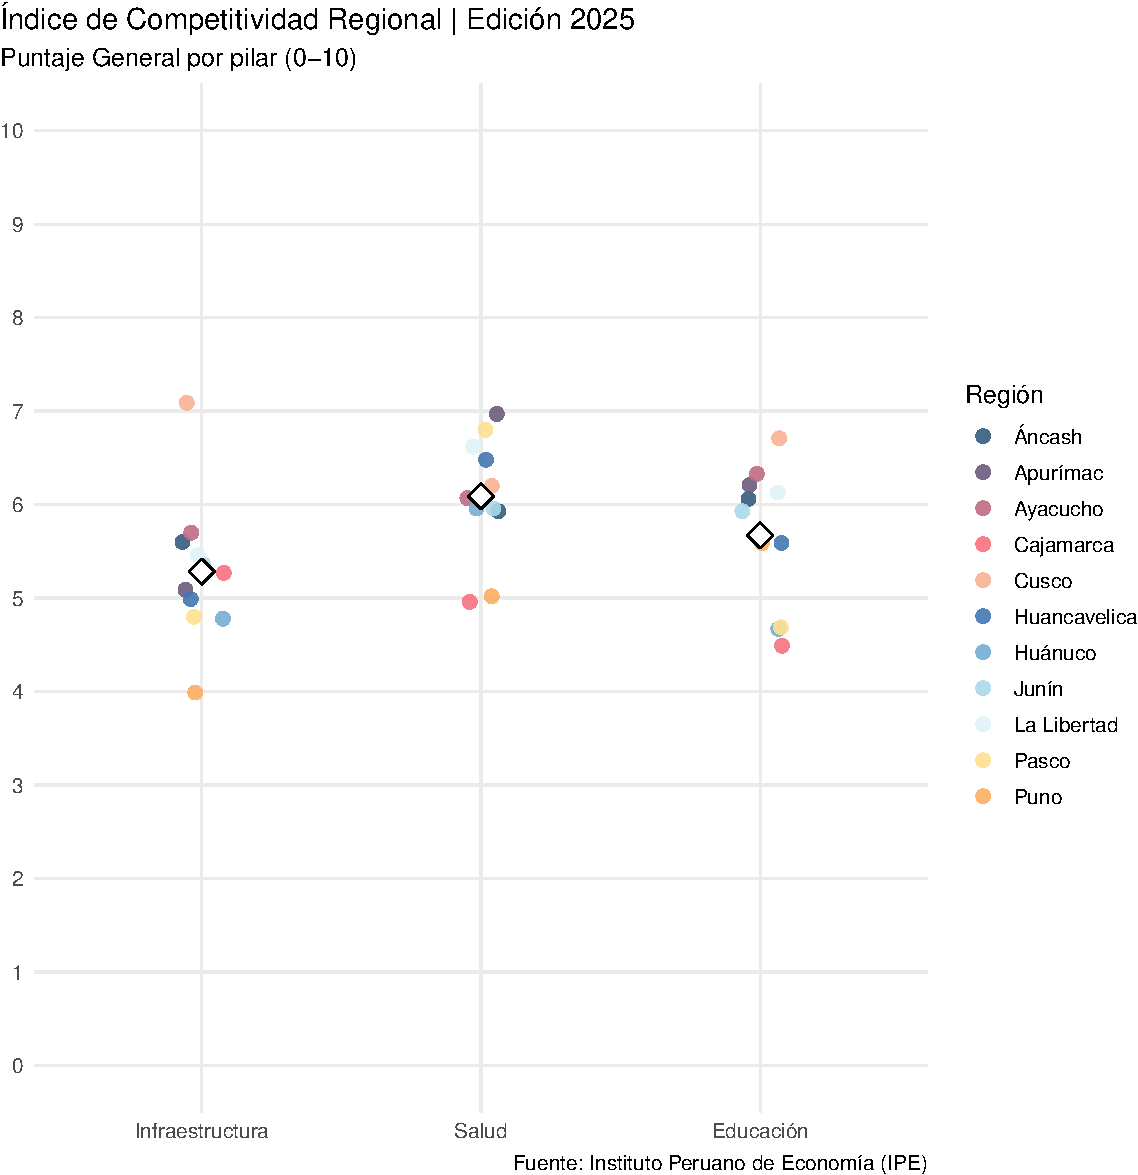
\includegraphics{Manual_files/figure-pdf/unnamed-chunk-25-1.pdf}

\textbf{Resultado esperado.} Dispersión para \textbf{Salud},
\textbf{Educación} (``EDU'') e \textbf{Infraestructura} (``INF'') en un
subconjunto que combina \textbf{grupo sierra}, una \textbf{región
específica} y una \textbf{exclusión}. El marcador del \textbf{promedio}
resalta como \textbf{referente} por pilar, mejorando la lectura
ejecutiva.

\subsection{\texorpdfstring{\textbf{general\_distribucion()}}{general\_distribucion()}}\label{general_distribucion}

\textbf{Distribución de puntajes (General o por pilares) en una edición}

Orientada a representar la \textbf{variabilidad} de los puntajes del
INCORE para \textbf{una edición} específica. A diferencia de un ranking,
que enfatiza el orden, general\_distribucion() enfatiza la
\textbf{distribución}: permite observar \textbf{medianas, rangos
intercuartílicos, colas y outliers} a través de \textbf{boxplots} o
\textbf{violines}, ya sea sobre el \textbf{índice general} (un único
eje) o sobre los \textbf{seis pilares} simultáneamente (seis ejes).

\subsubsection{\texorpdfstring{\textbf{Introducción}}{Introducción}}\label{introducciuxf3n-4}

El objetivo de general\_distribucion() es ofrecer una \textbf{lectura
estructurada de la dispersión} entre regiones. En contextos donde se
requiere comprender \textbf{heterogeneidad territorial}, esta
visualización ayuda a responder preguntas como: ¿qué tan amplia es la
variación entre regiones en cada pilar?, ¿en qué dimensiones los valores
se agrupan de forma compacta?, ¿cómo se compara la \textbf{media
nacional} con la distribución subnacional? La función trabaja
\textbf{exclusivamente} con filas cuya unidad es Puntaje del 0 al 10 y,
de forma consistente con el paquete, usa leer\_incore(\ldots,
agregar\_codigos = TRUE) para asegurar la disponibilidad de
\textbf{códigos canónicos} de pilar y región cuando correspondan.

\subsubsection{\texorpdfstring{\textbf{Parámetros}}{Parámetros}}\label{paruxe1metros-3}

La estrategia de uso se construye a partir de tres decisiones: (i)
\textbf{qué eje} se desea mostrar (``general'' vs ``pilares''), (ii)
\textbf{qué forma} de distribución se prefiere (``boxplot'' vs
``violin''), y (iii) \textbf{qué subconjunto} de regiones conviene
analizar (por grupos, exclusiones o mezcla de códigos/nombres). Sobre
ello, se aplican elecciones de \textbf{paleta} y elementos de
\textbf{lectura} como la \textbf{línea de promedio} y el
\textbf{jitter}.

\begin{itemize}
\item
  \textbf{edicion}: establece la \textbf{edición (año)} del INCORE a
  graficar, es un único valor numérico.

  Opciones y formato:

  \begin{itemize}
  \item
    integer(1)
  \item
    2016 \ldots{} 2025
  \end{itemize}
\item
  \textbf{modo}: define si la distribución se visualiza como \textbf{un
  solo eje} (índice general) o \textbf{seis ejes} (pilares).

  Opciones y formato:

  \begin{itemize}
  \item
    ``pilares'' (por defecto)
  \item
    ``general''
  \end{itemize}
\item
  \textbf{regiones}: delimita el \textbf{universo regional}, admite
  nombres, códigos, \textbf{grupos gr\_*}, e
  \textbf{inclusiones/exclusiones} con prefijo ``-''.

  Opciones y formato:

  \begin{itemize}
  \item
    ``ALL'' (todas las regiones)
  \item
    c(``REGION1'', ``REGION2'')
  \item
    c(``COD1'', ``COD2'')
  \item
    c(``gr\_costa'', ``gr\_sierra'', ``gr\_selva'')
  \item
    Exclusiones: ``-Lima*''
  \item
    Combinaciones mixtas: c(``gr\_costa'', ``La Libertad'', ``-Lima*'')
  \end{itemize}
\item
  \textbf{tipo}: el \textbf{estimador gráfico} de distribución.

  Opciones y formato:

  \begin{itemize}
  \item
    ``boxplot'' (por defecto, resalta mediana y cuartiles)
  \item
    ``violin'' (muestra densidad, útil con muchas observaciones)
  \end{itemize}
\item
  \textbf{jitter}: decide si superponer \textbf{puntos individuales}
  para evidenciar masa de datos o outliers locales.

  Opciones y formato:

  \begin{itemize}
  \item
    FALSE (por defecto)
  \item
    TRUE (añade puntos con alpha suave)
  \end{itemize}
\item
  \textbf{paleta}: paleta \textbf{discreta} de relleno, en modo =
  ``pilares'' se aplica \textbf{por pilar}, en modo = ``general'' el
  relleno es \textbf{único}.

  Opciones y formato:

  \begin{itemize}
  \item
    ``blues'' (por defecto)
  \item
    ``viridis''
  \item
    ``cividis''
  \end{itemize}
\item
  \textbf{linea\_promedio}: dibuja una \textbf{línea horizontal
  punteada} en el \textbf{promedio nacional} (calculado sobre regiones).

  Opciones y formato:

  \begin{itemize}
  \item
    TRUE (por defecto)
  \item
    FALSE
  \end{itemize}
\item
  \textbf{mostrar\_leyenda}: controla la visibilidad de leyenda
  (relevante solo en modo = ``pilares'').

  Opciones y formato:

  \begin{itemize}
  \item
    FALSE (por defecto)
  \item
    TRUE
  \end{itemize}
\end{itemize}

El parámetro \textbf{usar\_codigos} cumple un rol operativo (traducción
de códigos a nombres oficiales), normalmente se deja en TRUE para
mantener consistencia visual y editorial.

\subsubsection{\texorpdfstring{\textbf{Explicación
conceptual}}{Explicación conceptual}}\label{explicaciuxf3n-conceptual-3}

La función \textbf{lee} los datos de la edición solicitada con
\textbf{códigos} disponibles, \textbf{filtra} a Puntaje del 0 al 10 y
aplica, si corresponde, \textbf{resolución de grupos} y
\textbf{exclusiones} de regiones. En modo = ``general'', se construye
\textbf{un único eje} (código GEN) a partir del \textbf{índice general},
en modo = ``pilares'', se trabaja con los seis \textbf{códigos
canónicos} (ECO, LAB, INF, SAL, EDU, INS) y \textbf{se ordenan} los ejes
por una estadística robusta (p.~ej., mediana) para favorecer la lectura
comparativa. La \textbf{línea de promedio} agrega un referente nacional
por encima/dentro de la distribución, y la paleta \textbf{discreta}
garantiza legibilidad por pilar (o un estilo sobrio único en el caso
general). La salida es un objeto ggplot con escala \textbf{0--10} en el
eje vertical, coherente con el resto del paquete.

\subsubsection{\texorpdfstring{\textbf{Ejemplos}}{Ejemplos}}\label{ejemplos-3}

\paragraph{\texorpdfstring{\textbf{1) Distribución por pilares con
configuración por
defecto}}{1) Distribución por pilares con configuración por defecto}}\label{distribuciuxf3n-por-pilares-con-configuraciuxf3n-por-defecto}

\textbf{Se desea lo siguiente:} visualizar la distribución del
\textbf{puntaje General} por cada pilar para una edición reciente, sin
filtros adicionales.

\begin{Shaded}
\begin{Highlighting}[]
\NormalTok{g1 }\OtherTok{\textless{}{-}} \FunctionTok{general\_distribucion}\NormalTok{(}
  \AttributeTok{edicion =} \DecValTok{2025}\NormalTok{,}
  \AttributeTok{modo    =} \StringTok{"pilares"}\NormalTok{,}
  \AttributeTok{regiones =} \StringTok{"ALL"}
\NormalTok{)}
\NormalTok{g1}
\end{Highlighting}
\end{Shaded}

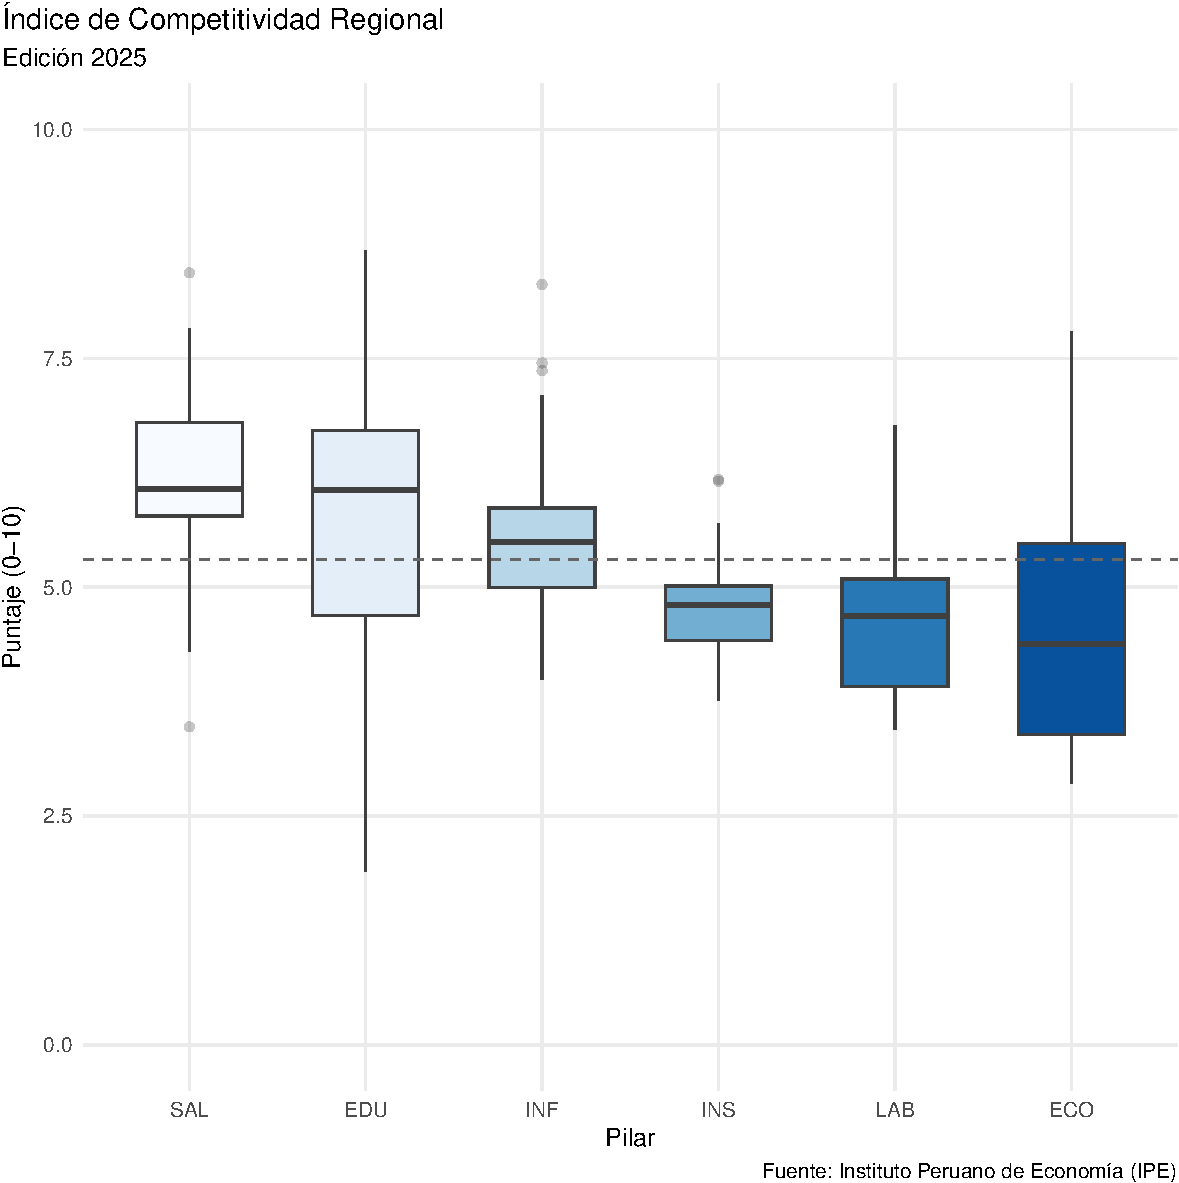
\includegraphics{Manual_files/figure-pdf/unnamed-chunk-26-1.pdf}

\textbf{Resultado esperado.} Seis ejes
(``ECO'',``LAB'',``INF'',``SAL'',``EDU'',``INS'') con \textbf{boxplots}
(o violines, según tipo) y \textbf{línea de promedio} nacional. Permite
detectar de inmediato pilares con \textbf{dispersión alta} frente a
otros más \textbf{compactos}.

\paragraph{\texorpdfstring{\textbf{2) Índice General (un solo eje) con
jitter{]} y
promedio}}{2) Índice General (un solo eje) con jitter{]} y promedio}}\label{uxedndice-general-un-solo-eje-con-jitter-y-promedio}

\textbf{Se desea lo siguiente:} observar la \textbf{variabilidad
nacional} del índice general, con puntos individuales para evidenciar
posibles outliers.

\begin{Shaded}
\begin{Highlighting}[]
\NormalTok{g2 }\OtherTok{\textless{}{-}} \FunctionTok{general\_distribucion}\NormalTok{(}
  \AttributeTok{edicion =} \DecValTok{2025}\NormalTok{,}
  \AttributeTok{modo    =} \StringTok{"general"}\NormalTok{,}
  \AttributeTok{tipo    =} \StringTok{"boxplot"}\NormalTok{,}
  \AttributeTok{jitter  =} \ConstantTok{TRUE}\NormalTok{,}
  \AttributeTok{linea\_promedio =} \ConstantTok{TRUE}
\NormalTok{)}
\NormalTok{g2}
\end{Highlighting}
\end{Shaded}

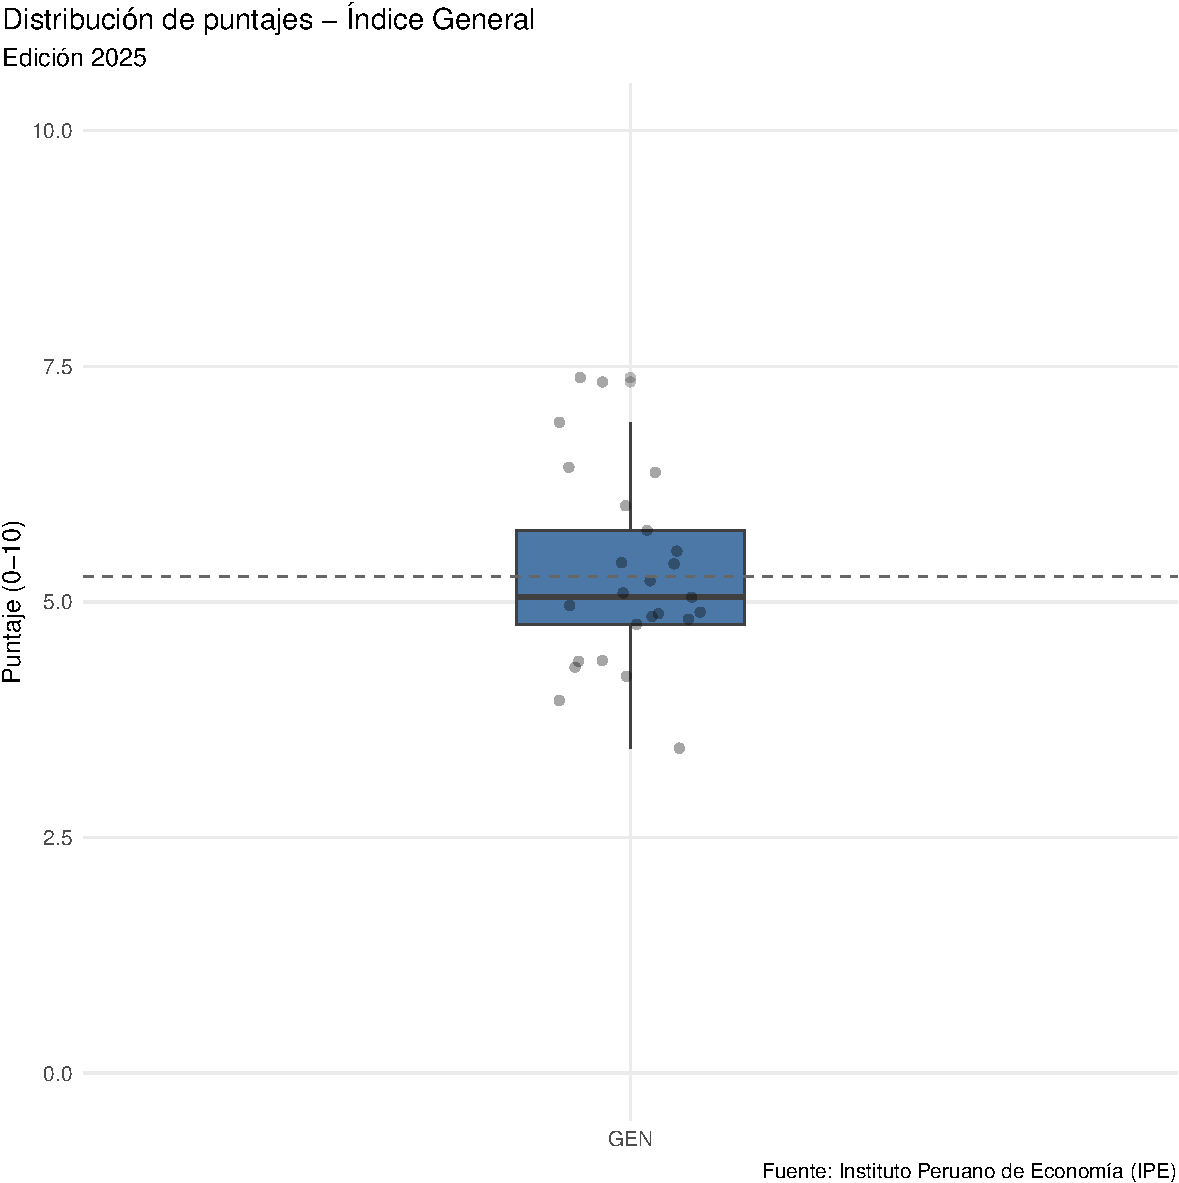
\includegraphics{Manual_files/figure-pdf/unnamed-chunk-27-1.pdf}

\textbf{Resultado esperado.} Un eje único etiquetado como ``GEN'', el
\textbf{boxplot} resume la distribución y el \textbf{jitter} muestra el
posicionamiento puntual de cada región. La \textbf{línea de promedio}
sirve de referencia global.

\paragraph{\texorpdfstring{\textbf{3) Subconjunto costero con exclusión
de Lima* y paleta
accesible}}{3) Subconjunto costero con exclusión de Lima* y paleta accesible}}\label{subconjunto-costero-con-exclusiuxf3n-de-lima-y-paleta-accesible}

\textbf{Se desea lo siguiente:} analizar la distribución de pilares solo
en la \textbf{costa}, excluyendo \textbf{Lima}*, y mejorar la
accesibilidad cromática.

\begin{Shaded}
\begin{Highlighting}[]
\NormalTok{g3 }\OtherTok{\textless{}{-}} \FunctionTok{general\_distribucion}\NormalTok{(}
  \AttributeTok{edicion =} \DecValTok{2025}\NormalTok{,}
  \AttributeTok{modo    =} \StringTok{"pilares"}\NormalTok{,}
  \AttributeTok{regiones =} \FunctionTok{c}\NormalTok{(}\StringTok{"gr\_costa"}\NormalTok{, }\StringTok{"{-}Lima*"}\NormalTok{),}
  \AttributeTok{tipo    =} \StringTok{"violin"}\NormalTok{,}
  \AttributeTok{paleta  =} \StringTok{"cividis"}\NormalTok{,}
  \AttributeTok{mostrar\_leyenda =} \ConstantTok{TRUE}
\NormalTok{)}
\NormalTok{g3}
\end{Highlighting}
\end{Shaded}

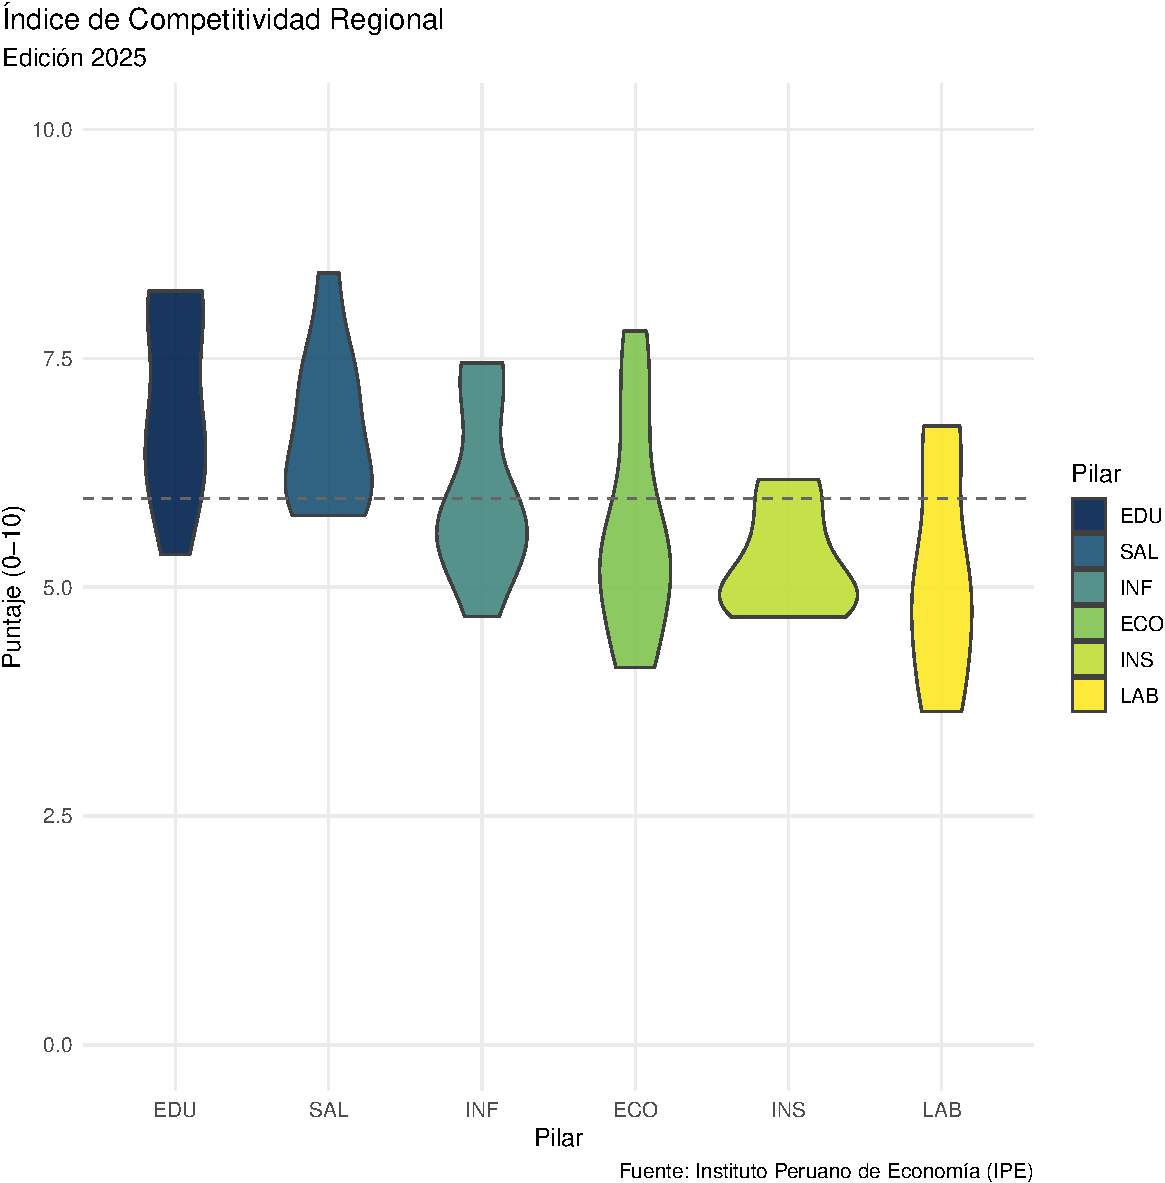
\includegraphics{Manual_files/figure-pdf/unnamed-chunk-28-1.pdf}

\textbf{Resultado esperado.} Seis violines con distribución \textbf{sin
Lima}* (para evitar que su peso estructural distorsione la lectura). La
paleta ``cividis'' favorece la \textbf{distinguibilidad} en proyección e
impresión.

\paragraph{\texorpdfstring{\textbf{4) Foco en tres pilares clave con
jitter fino y paleta
perceptual}}{4) Foco en tres pilares clave con jitter fino y paleta perceptual}}\label{foco-en-tres-pilares-clave-con-jitter-fino-y-paleta-perceptual}

\textbf{Se desea lo siguiente:} concentrar la lectura en
\textbf{Educación}, \textbf{Infraestructura} y \textbf{Salud} con
separación adicional de puntos.

\begin{Shaded}
\begin{Highlighting}[]
\NormalTok{g4 }\OtherTok{\textless{}{-}} \FunctionTok{general\_distribucion}\NormalTok{(}
  \AttributeTok{edicion =} \DecValTok{2025}\NormalTok{,}
  \AttributeTok{modo    =} \StringTok{"pilares"}\NormalTok{,}
  \AttributeTok{regiones =} \StringTok{"ALL"}\NormalTok{,}
  \AttributeTok{tipo    =} \StringTok{"boxplot"}\NormalTok{,}
  \AttributeTok{jitter  =} \ConstantTok{TRUE}\NormalTok{,}
  \AttributeTok{paleta  =} \StringTok{"viridis"}\NormalTok{,}
  \AttributeTok{mostrar\_leyenda =} \ConstantTok{TRUE}
\NormalTok{)}

\NormalTok{g4}
\end{Highlighting}
\end{Shaded}

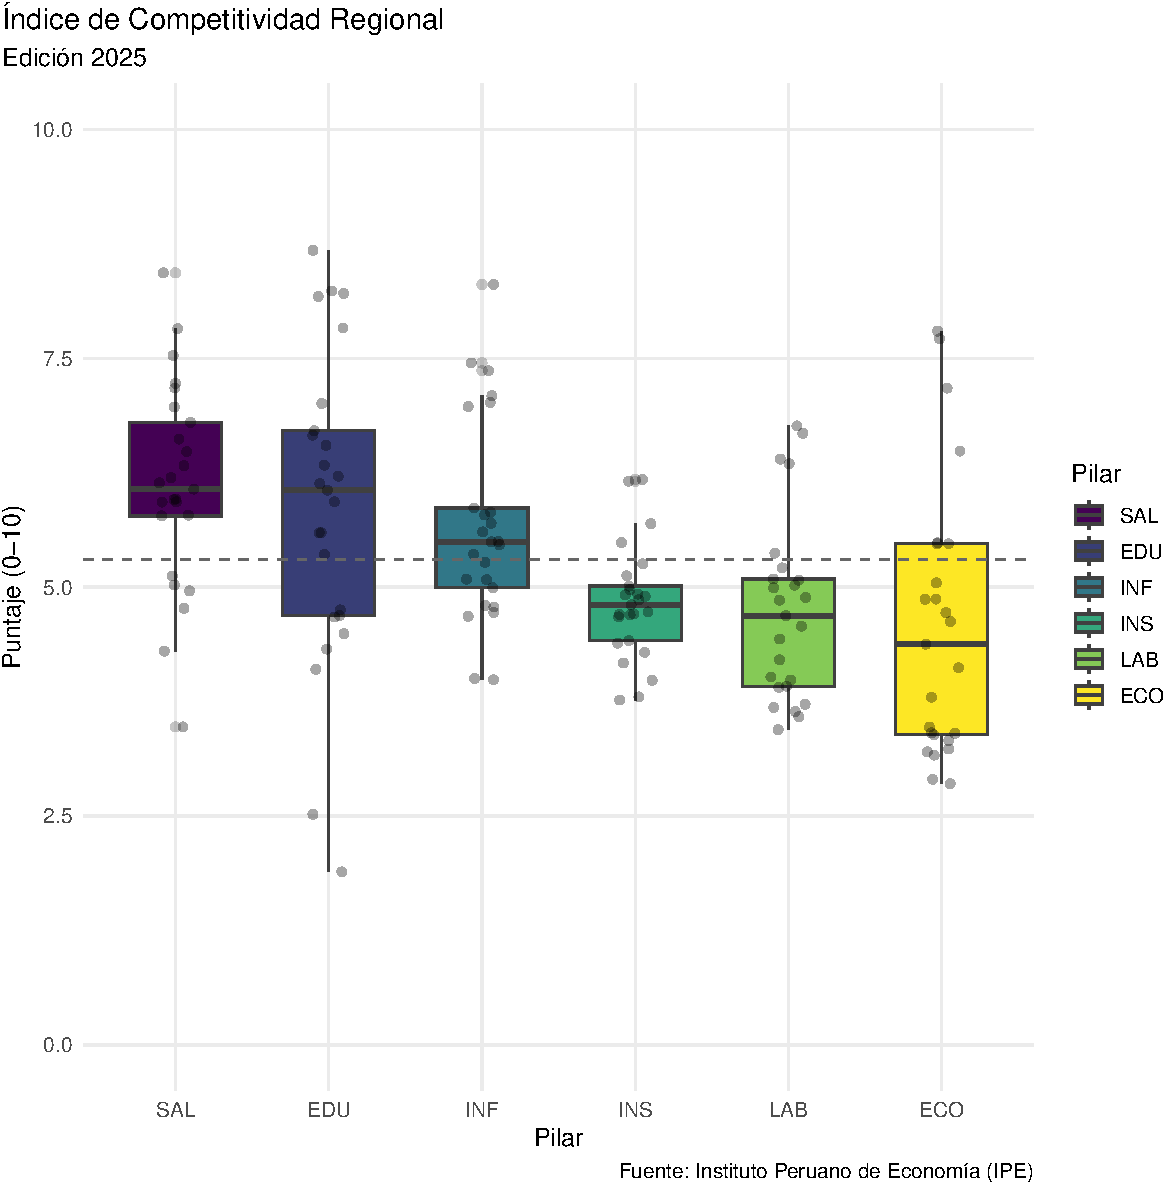
\includegraphics{Manual_files/figure-pdf/unnamed-chunk-29-1.pdf}

\textbf{Resultado esperado.} Boxplots por pilar con \textbf{puntos}
superpuestos, la paleta ``viridis'' mantiene \textbf{contraste}.

\paragraph{\texorpdfstring{\textbf{5) Comparación ``bloque mixto''
(grupo + nombres) con línea de promedio
activada}}{5) Comparación ``bloque mixto'' (grupo + nombres) con línea de promedio activada}}\label{comparaciuxf3n-bloque-mixto-grupo-nombres-con-luxednea-de-promedio-activada}

\textbf{Se desea lo siguiente:} comparar un \textbf{bloque mixto}
formado por gr\_sierra y dos regiones específicas, manteniendo la
referencia nacional.

\begin{Shaded}
\begin{Highlighting}[]
\NormalTok{g5 }\OtherTok{\textless{}{-}} \FunctionTok{general\_distribucion}\NormalTok{(}
  \AttributeTok{edicion =} \DecValTok{2025}\NormalTok{,}
  \AttributeTok{modo    =} \StringTok{"pilares"}\NormalTok{,}
  \AttributeTok{regiones =} \FunctionTok{c}\NormalTok{(}\StringTok{"gr\_sierra"}\NormalTok{, }\StringTok{"La Libertad"}\NormalTok{),}
  \AttributeTok{tipo    =} \StringTok{"violin"}\NormalTok{,}
  \AttributeTok{paleta  =} \StringTok{"blues"}\NormalTok{,}
  \AttributeTok{linea\_promedio =} \ConstantTok{TRUE}\NormalTok{,}
  \AttributeTok{mostrar\_leyenda =} \ConstantTok{TRUE}
\NormalTok{)}
\NormalTok{g5}
\end{Highlighting}
\end{Shaded}

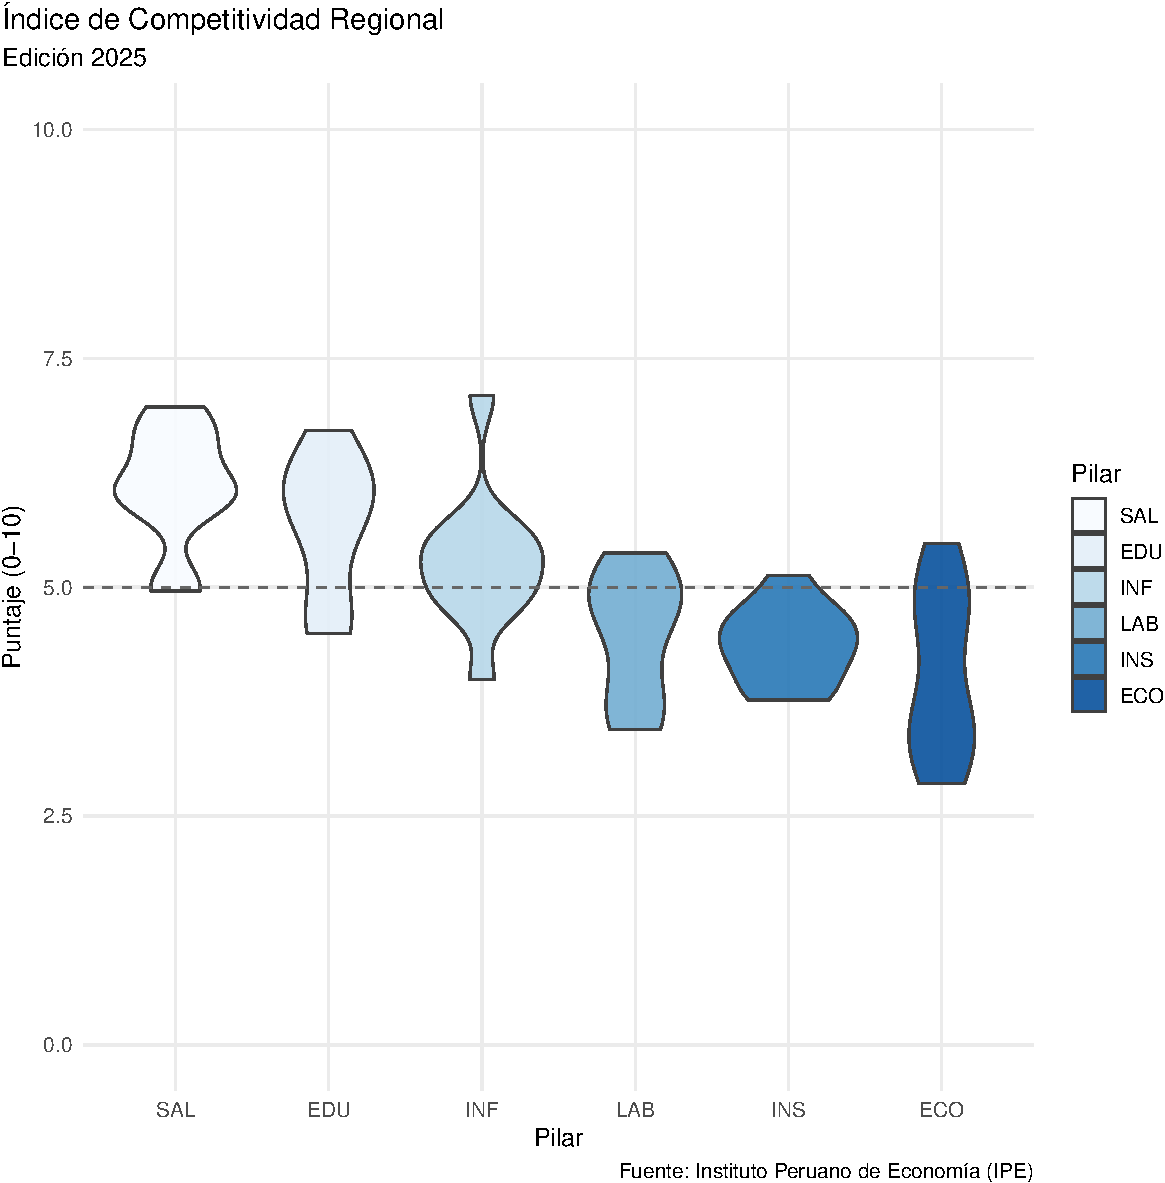
\includegraphics{Manual_files/figure-pdf/unnamed-chunk-30-1.pdf}

\textbf{Resultado esperado.} Violines por pilar con énfasis en un
\textbf{bloque heterogéneo} (grupo + regiones puntuales). La
\textbf{línea de promedio} refuerza la comparación ``por encima/por
debajo'' del referente nacional, útil para mensajes ejecutivos.

\subsection{\texorpdfstring{\textbf{general\_heatmap()}}{general\_heatmap()}}\label{general_heatmap}

\textbf{Mapa de calor del puntaje General por región en múltiples
ediciones}

\subsubsection{\texorpdfstring{\textbf{Introducción}}{Introducción}}\label{introducciuxf3n-5}

general\_heatmap() resuelve un problema habitual en el análisis
longitudinal: \textbf{comparar la evolución del puntaje General (0--10)
por región a lo largo de varias ediciones}. La representación en
\textbf{mapa de calor} condensa, en una sola figura, tres componentes:
\textbf{regiones} (filas), \textbf{ediciones} (columnas) y
\textbf{magnitud} del puntaje (color). Esta composición facilita
detectar \textbf{tendencias} (mejoras o retrocesos),
\textbf{persistencias} (niveles consistentemente altos o bajos) y
\textbf{rupturas} (cambios bruscos entre ediciones). La función trabaja
exclusivamente con filas cuyo pilar \textbf{comienza con} ``Índice de
Competitividad Regional'' (es decir, el \textbf{índice general}), y
excluye ``Perú'' para conservar el foco comparativo a nivel regional.

\subsubsection{\texorpdfstring{\textbf{Parámetros}}{Parámetros}}\label{paruxe1metros-4}

El uso práctico de general\_heatmap() se articula en tres decisiones:
(i) \textbf{rango de ediciones} a mostrar, (ii) \textbf{universo de
regiones} (total o subconjunto) y (iii) \textbf{orden de las filas} de
cara a la lectura. Sobre ello, se elige la \textbf{paleta continua} de
color, se decide si \textbf{anotar valores} en cada celda y si
\textbf{exhibir la leyenda}.

\begin{itemize}
\item
  \textbf{ediciones}: define el \textbf{conjunto de ediciones} a
  visualizar, requiere \textbf{al menos dos años}.

  Opciones y formato:

  \begin{itemize}
  \item
    integer vector con longitud ≥ 2
  \item
    Rangos: 2019:2025
  \item
    Discretos: c(2018, 2020, 2022, 2024)
  \end{itemize}
\item
  \textbf{regiones}: establece el \textbf{universo regional}, admite
  nombres, códigos y, si el paquete lo dispone, \textbf{grupos gr\_*} y
  \textbf{exclusiones} por prefijo ``-''.

  Opciones y formato:

  \begin{itemize}
  \item
    ``ALL'' (todas las regiones)
  \item
    c(``Lima*'', ``Arequipa'', ``Cusco'') (nombres o patrones)
  \item
    c(``MOQ'', ``ARE'', ``CUS'') (códigos, si están definidos en
    catálogos)
  \item
    c(``gr\_costa'', ``gr\_sierra'') (grupos predefinidos)
  \item
    Exclusiones por patrón: ``-Lima*''
  \item
    Combinaciones mixtas: c(``gr\_costa'', ``La Libertad'', ``-Lima*'')
  \end{itemize}
\item
  \textbf{ordenar}: especifica el \textbf{criterio de orden} de las
  filas (regiones) para favorecer la lectura comparativa.

  Opciones y formato:

  \begin{itemize}
  \item
    ``ninguno'' (orden alfabético)
  \item
    ``por\_ultimo'' (según puntaje de la \textbf{última} edición del
    rango)
  \item
    ``por\_promedio'' (según \textbf{promedio} del puntaje en el rango
    de ediciones)
  \end{itemize}
\item
  \textbf{paleta}: selecciona la \textbf{paleta continua} para el mapeo
  0--10.

  Opciones y formato:

  \begin{itemize}
  \item
    ``blues'' (por defecto, progresión fría sobria)
  \item
    ``viridis'' (perceptualmente uniforme)
  \item
    ``cividis'' (accesible en proyección e impresión)
  \item
    ``magma'' (contraste alto, útil para resaltar extremos)
  \end{itemize}
\item
  \textbf{anotar}: decide si \textbf{imprimir el valor} dentro de cada
  celda.

  Opciones y formato:

  \begin{itemize}
  \item
    FALSE (por defecto)
  \item
    TRUE (muestra valores con dos decimales)
  \end{itemize}
\item
  \textbf{mostrar\_leyenda}: controla la \textbf{visibilidad de la
  leyenda} de colores.

  Opciones y formato:

  \begin{itemize}
  \item
    TRUE
  \item
    FALSE
  \end{itemize}
\end{itemize}

El parámetro \textbf{usar\_codigos} cumple un rol operativo: cuando es
TRUE, traduce códigos de regiones a \textbf{nombres oficiales} para
mantener consistencia editorial (normalmente se deja activado).

\subsubsection{\texorpdfstring{\textbf{Explicación
conceptual}}{Explicación conceptual}}\label{explicaciuxf3n-conceptual-4}

La función \textbf{lee} el conjunto de ediciones solicitadas,
\textbf{filtra} únicamente el \textbf{índice general} (descartando el
agregado nacional ``Perú''), y \textbf{consolida} un valor por (región,
edición) para garantizar unicidad en cada celda del mapa. Luego
\textbf{ordena} las filas según el criterio indicado: alfabético, por el
valor de la \textbf{última edición} (adecuado cuando el interés es la
situación más reciente) o por el \textbf{promedio} a lo largo del
período (útil para lecturas de \textbf{desempeño sostenido}). Finalmente
aplica una \textbf{paleta continua} con límites \textbf{0--10} y, si se
solicita, \textbf{anota} el valor en cada celda, lo que puede ser
conveniente en matrices pequeñas o en cortes enfocados.

\subsubsection{\texorpdfstring{\textbf{Ejemplos}}{Ejemplos}}\label{ejemplos-4}

\paragraph{\texorpdfstring{\textbf{1) Panorama básico por ediciones
(orden alfabético, paleta por
defecto)}}{1) Panorama básico por ediciones (orden alfabético, paleta por defecto)}}\label{panorama-buxe1sico-por-ediciones-orden-alfabuxe9tico-paleta-por-defecto}

\textbf{Se desea lo siguiente:} visualizar la evolución 2020--2025 para
todas las regiones, priorizando una lectura sobria.

\begin{Shaded}
\begin{Highlighting}[]
\NormalTok{h1 }\OtherTok{\textless{}{-}} \FunctionTok{general\_heatmap}\NormalTok{(}
  \AttributeTok{ediciones =} \DecValTok{2020}\SpecialCharTok{:}\DecValTok{2025}\NormalTok{,}
  \AttributeTok{regiones  =} \StringTok{"ALL"}\NormalTok{,}
  \AttributeTok{ordenar   =} \StringTok{"ninguno"}\NormalTok{,}
  \AttributeTok{paleta    =} \StringTok{"blues"}
\NormalTok{)}
\NormalTok{h1}
\end{Highlighting}
\end{Shaded}

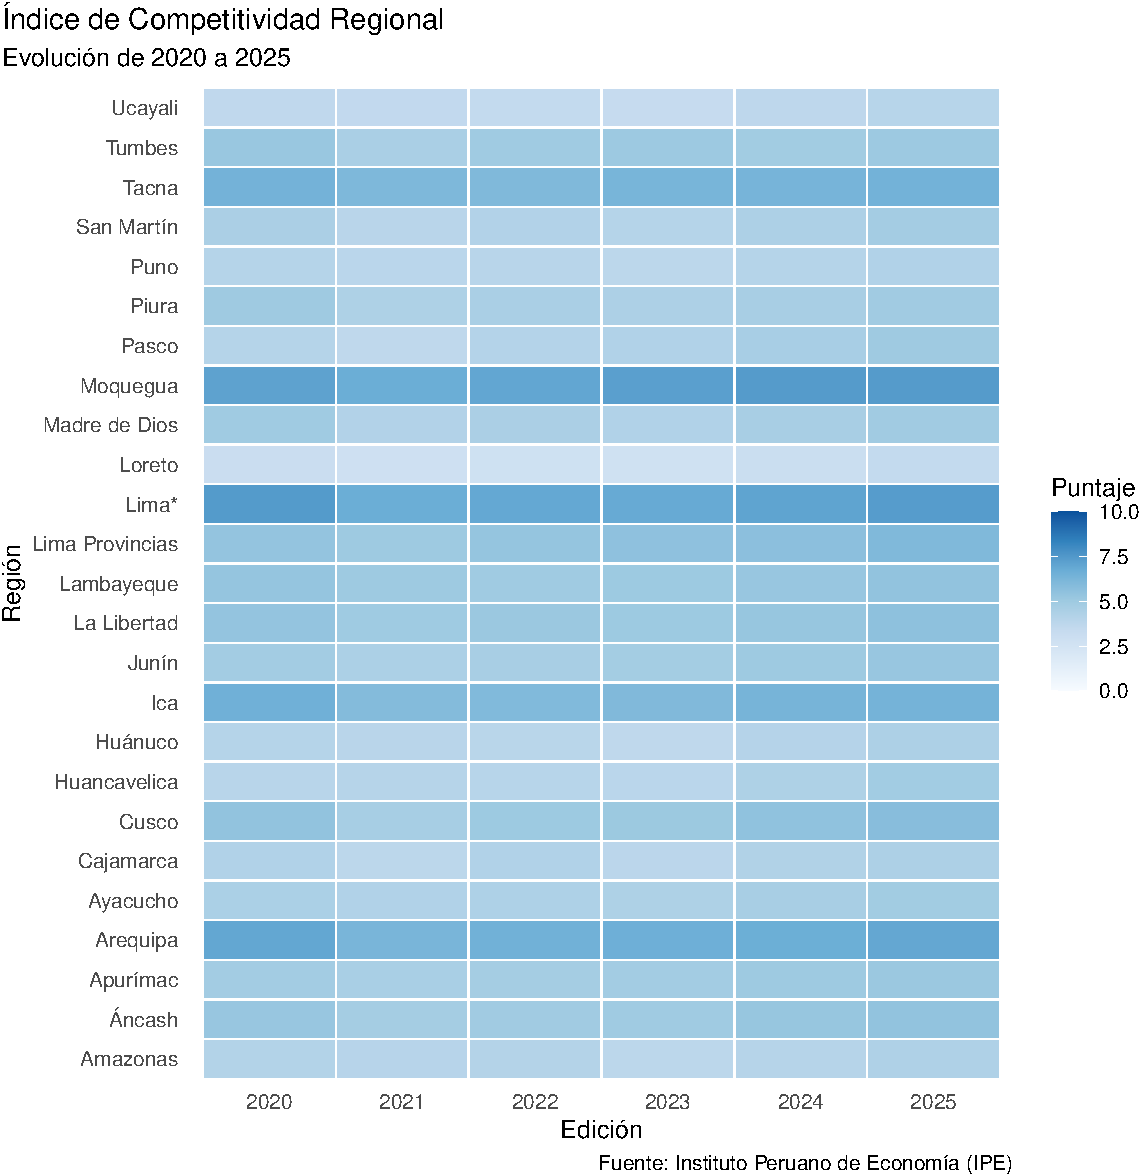
\includegraphics{Manual_files/figure-pdf/unnamed-chunk-31-1.pdf}

\textbf{Resultado esperado.} Mapa de calor con filas alfabéticas y
columnas 2020\ldots2025, la progresión ``blues'' facilita distinguir
niveles sin saturar.

\paragraph{\texorpdfstring{\textbf{2) Enfoque en la foto más reciente
(orden por última
edición)}}{2) Enfoque en la foto más reciente (orden por última edición)}}\label{enfoque-en-la-foto-muxe1s-reciente-orden-por-uxfaltima-ediciuxf3n}

\textbf{Se desea lo siguiente:} ordenar las regiones según su valor en
la edición más reciente del rango.

\begin{Shaded}
\begin{Highlighting}[]
\NormalTok{h2 }\OtherTok{\textless{}{-}} \FunctionTok{general\_heatmap}\NormalTok{(}
  \AttributeTok{ediciones =} \DecValTok{2019}\SpecialCharTok{:}\DecValTok{2025}\NormalTok{,}
  \AttributeTok{regiones  =} \StringTok{"ALL"}\NormalTok{,}
  \AttributeTok{ordenar   =} \StringTok{"por\_ultimo"}\NormalTok{,}
  \AttributeTok{paleta    =} \StringTok{"viridis"}\NormalTok{,}
  \AttributeTok{mostrar\_leyenda =} \ConstantTok{TRUE}
\NormalTok{)}
\NormalTok{h2}
\end{Highlighting}
\end{Shaded}

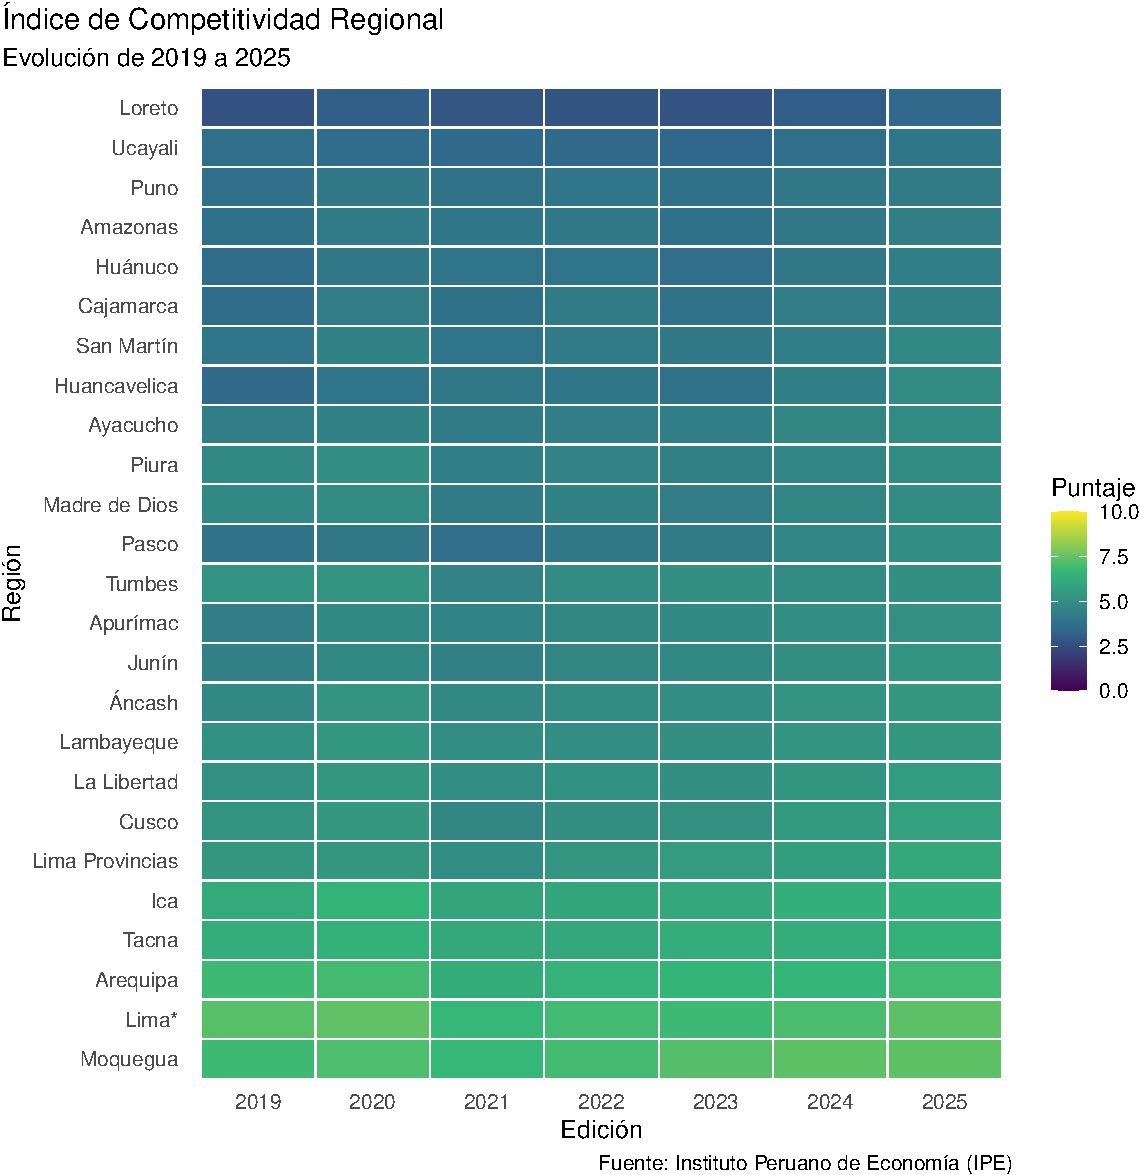
\includegraphics{Manual_files/figure-pdf/unnamed-chunk-32-1.pdf}

\textbf{Resultado esperado.} Filas ordenadas de mayor a menor
\textbf{según 2025}, útil para destacar posiciones actuales y evaluar
trayectorias relativas.

\paragraph{\texorpdfstring{\textbf{3) Subconjunto con grupo y exclusión
(anotando
valores)}}{3) Subconjunto con grupo y exclusión (anotando valores)}}\label{subconjunto-con-grupo-y-exclusiuxf3n-anotando-valores}

\textbf{Se desea lo siguiente:} comparar solo la \textbf{costa}
excluyendo \textbf{Lima}* y \textbf{anotar} los puntajes para un
seguimiento fino.

\begin{Shaded}
\begin{Highlighting}[]
\NormalTok{h3 }\OtherTok{\textless{}{-}} \FunctionTok{general\_heatmap}\NormalTok{(}
  \AttributeTok{ediciones =} \DecValTok{2021}\SpecialCharTok{:}\DecValTok{2025}\NormalTok{,}
  \AttributeTok{regiones  =} \FunctionTok{c}\NormalTok{(}\StringTok{"gr\_costa"}\NormalTok{, }\StringTok{"{-}Lima*"}\NormalTok{),}
  \AttributeTok{ordenar   =} \StringTok{"por\_promedio"}\NormalTok{,}
  \AttributeTok{paleta    =} \StringTok{"cividis"}\NormalTok{,}
  \AttributeTok{anotar    =} \ConstantTok{TRUE}\NormalTok{,}
  \AttributeTok{mostrar\_leyenda =} \ConstantTok{TRUE}
\NormalTok{)}
\NormalTok{h3}
\end{Highlighting}
\end{Shaded}

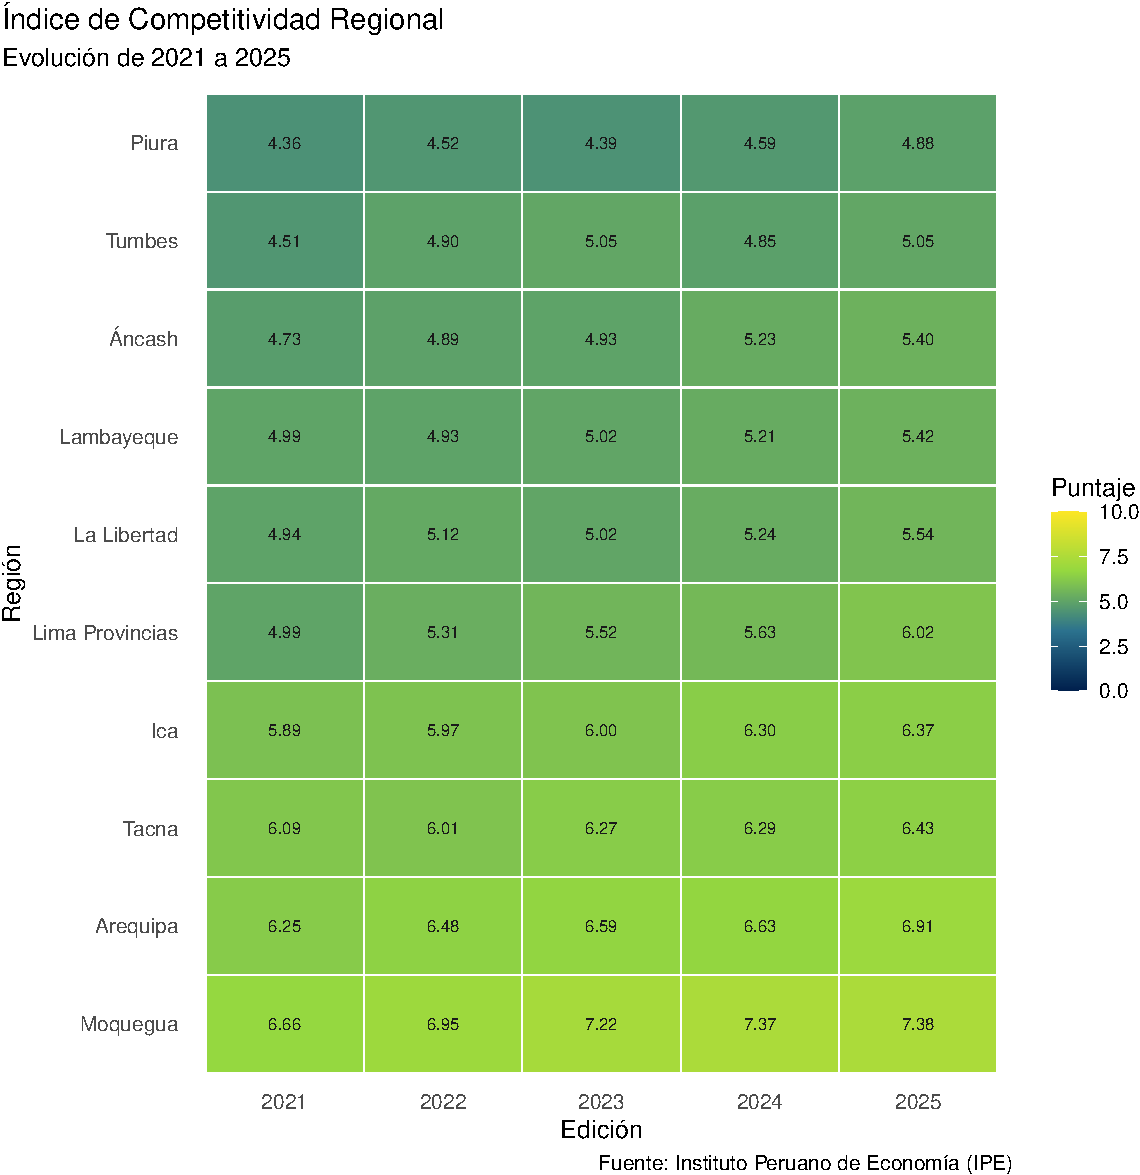
\includegraphics{Manual_files/figure-pdf/unnamed-chunk-33-1.pdf}

\textbf{Resultado esperado.} Filas ordenadas por el \textbf{promedio
2021--2025} de la costa \textbf{sin Lima}*, con valores impresos en cada
celda, la paleta ``cividis'' favorece la distinguibilidad en proyección.

\paragraph{\texorpdfstring{\textbf{4) Corte enfocado con códigos/nombres
y contraste
alto}}{4) Corte enfocado con códigos/nombres y contraste alto}}\label{corte-enfocado-con-cuxf3digosnombres-y-contraste-alto}

\textbf{Se desea lo siguiente:} mostrar 2022--2025 para un subconjunto
mixto (códigos + nombres) con contraste cromático alto.

\begin{Shaded}
\begin{Highlighting}[]
\NormalTok{h4 }\OtherTok{\textless{}{-}} \FunctionTok{general\_heatmap}\NormalTok{(}
  \AttributeTok{ediciones =} \DecValTok{2022}\SpecialCharTok{:}\DecValTok{2025}\NormalTok{,}
  \AttributeTok{regiones  =} \FunctionTok{c}\NormalTok{(}\StringTok{"MOQ"}\NormalTok{, }\StringTok{"Arequipa"}\NormalTok{, }\StringTok{"La Libertad"}\NormalTok{, }\StringTok{"Cusco"}\NormalTok{),}
  \AttributeTok{ordenar   =} \StringTok{"por\_ultimo"}\NormalTok{,}
  \AttributeTok{paleta    =} \StringTok{"magma"}\NormalTok{,}
  \AttributeTok{anotar    =} \ConstantTok{FALSE}
\NormalTok{)}
\NormalTok{h4}
\end{Highlighting}
\end{Shaded}

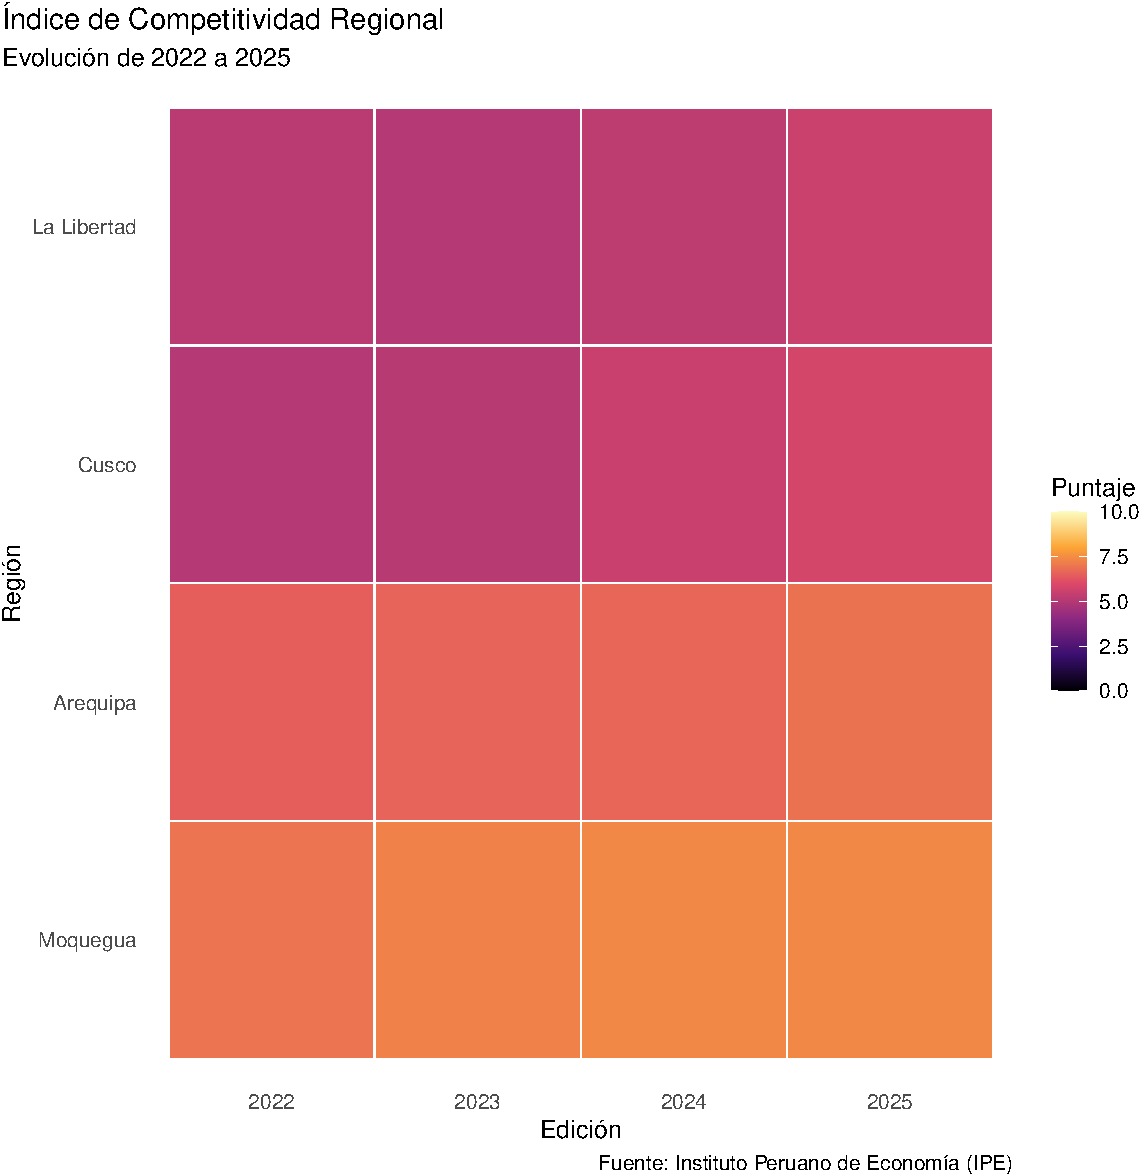
\includegraphics{Manual_files/figure-pdf/unnamed-chunk-34-1.pdf}

\textbf{Resultado esperado.} Mapa compacto que prioriza la lectura por
\textbf{última edición} y resalta extremos con ``magma'', útil para
resúmenes ejecutivos.

\paragraph{\texorpdfstring{\textbf{5) Serie discontinua de ediciones con
orden por
promedio}}{5) Serie discontinua de ediciones con orden por promedio}}\label{serie-discontinua-de-ediciones-con-orden-por-promedio}

\textbf{Se desea lo siguiente:} evaluar un patrón \textbf{no anual}
(años alternos) y ordenar por \textbf{desempeño sostenido}.

\begin{Shaded}
\begin{Highlighting}[]
\NormalTok{h5 }\OtherTok{\textless{}{-}} \FunctionTok{general\_heatmap}\NormalTok{(}
  \AttributeTok{ediciones =} \FunctionTok{c}\NormalTok{(}\DecValTok{2017}\NormalTok{, }\DecValTok{2019}\NormalTok{, }\DecValTok{2021}\NormalTok{, }\DecValTok{2023}\NormalTok{, }\DecValTok{2025}\NormalTok{),}
  \AttributeTok{regiones  =} \StringTok{"ALL"}\NormalTok{,}
  \AttributeTok{ordenar   =} \StringTok{"por\_promedio"}\NormalTok{,}
  \AttributeTok{paleta    =} \StringTok{"viridis"}\NormalTok{,}
  \AttributeTok{anotar    =} \ConstantTok{FALSE}\NormalTok{,}
  \AttributeTok{mostrar\_leyenda =} \ConstantTok{TRUE}
\NormalTok{)}
\NormalTok{h5}
\end{Highlighting}
\end{Shaded}

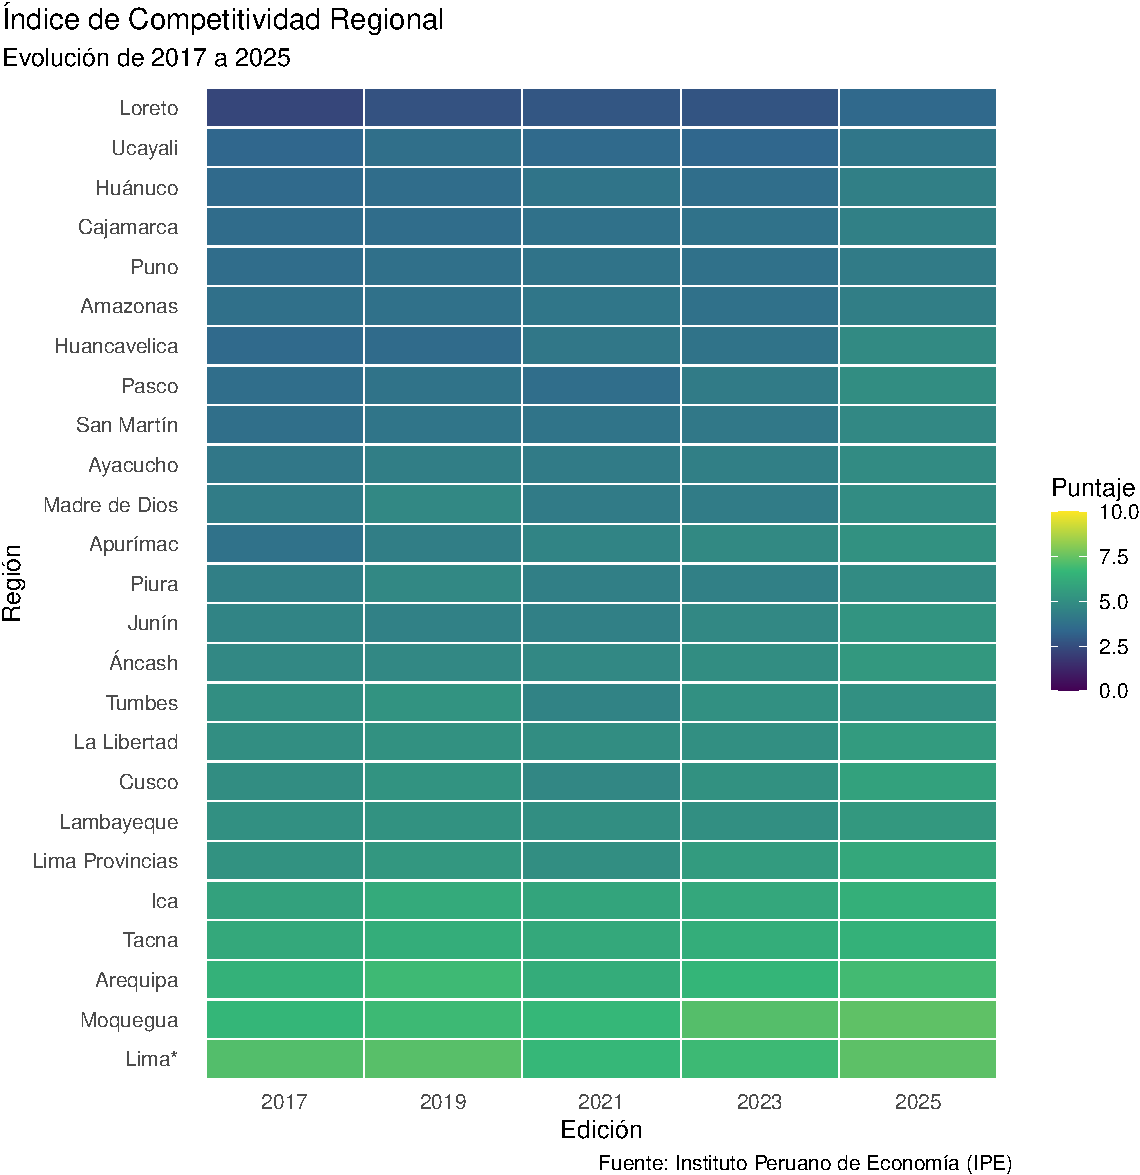
\includegraphics{Manual_files/figure-pdf/unnamed-chunk-35-1.pdf}

\textbf{Resultado esperado.} Filas ordenadas por el \textbf{promedio} en
una serie discontinua, lo que ayuda a identificar regiones con
\textbf{rendimiento consistente} a lo largo del tiempo.

\subsection{\texorpdfstring{\textbf{general\_largo()}}{general\_largo()}}\label{general_largo}

\textbf{Evolución del puntaje General (líneas) por región y/o por pilar}

Esta función integra la familia de visualizaciones general\_* y está
diseñada para \textbf{series de tiempo} del \textbf{puntaje General
(0--10)} del INCORE cuando se dispone de \textbf{dos o más ediciones}.
Ofrece dos enfoques complementarios:

\begin{itemize}
\item
  modo = ``general'': una \textbf{línea por región} del \textbf{índice
  general} (filas cuyo pilar inicia con ``Índice de Competitividad
  Regional'' e indicador == ``General'').
\item
  modo = ``pilares'': \textbf{líneas por región} con \textbf{facetado
  por pilar}, utilizando indicador == ``General'' en cada pilar.
\end{itemize}

\subsubsection{\texorpdfstring{\textbf{Introducción}}{Introducción}}\label{introducciuxf3n-6}

general\_largo() resuelve la necesidad de \textbf{observar
trayectorias}: cómo evolucionan las regiones en el \textbf{índice
general} o, alternativamente, cómo se mueven \textbf{en cada pilar} a lo
largo del tiempo. Es especialmente útil para identificar
\textbf{convergencias} o \textbf{divergencias} regionales,
\textbf{rupturas} (cambios abruptos entre ediciones),
\textbf{persistencias} (tendencias sostenidas) y \textbf{liderazgos}
emergentes. En modo = ``pilares'', el \textbf{facetado} permite
comparar, en paralelo, si la historia de una misma región es similar o
distinta según el pilar considerado. El eje vertical se mantiene en
\textbf{0--10} para asegurar comparabilidad, y la estética de color por
región preserva la identidad visual en todas las ediciones.

El argumento usar\_codigos (secundario) facilita la \textbf{traducción
de códigos} a nombres oficiales en regiones/pilares para mantener
consistencia editorial y legibilidad en etiquetas y leyendas.

\subsubsection{\texorpdfstring{\textbf{Parámetros}}{Parámetros}}\label{paruxe1metros-5}

El uso práctico se apoya en tres decisiones: (i) \textbf{rango de
ediciones} a estudiar, (ii) \textbf{nivel de análisis} (índice general
vs.~pilares) y (iii) \textbf{universo de regiones} (total o
subconjunto). Sobre estas, se elige la \textbf{paleta} y si conviene
\textbf{marcar puntos} en las líneas.

\begin{itemize}
\item
  \textbf{ediciones}: determina las \textbf{ediciones (años)} a
  graficar, requiere \textbf{al menos dos}.

  Opciones y formato:

  \begin{itemize}
  \item
    integer vector con longitud ≥ 2
  \item
    Rangos: 2020:2025
  \item
    Discretos: c(2018, 2020, 2022, 2024)
  \end{itemize}
\item
  \textbf{regiones}: define el \textbf{universo regional}, admite
  nombres, códigos, \textbf{grupos gr\_*} y \textbf{exclusiones} con
  prefijo ``-''.

  Opciones y formato:

  \begin{itemize}
  \item
    ``ALL'' (todas las regiones)
  \item
    c(``REGION1'', ``REGION2'')
  \item
    c(``COD1'', ``COD2'')
  \item
    c(``gr\_costa'', ``gr\_sierra'', ``gr\_selva'')
  \item
    Exclusiones: ``-Lima*''
  \item
    Combinaciones mixtas: c(``gr\_costa'', ``La Libertad'', ``-Lima*'')
  \end{itemize}
\item
  \textbf{modo}: establece el \textbf{nivel de análisis} temporal.

  Opciones y formato:

  \begin{itemize}
  \item
    ``general'' (una línea por región, índice general)
  \item
    ``pilares'' (líneas por región, \textbf{facetado} por los seis
    pilares)
  \end{itemize}
\item
  \textbf{pilares} \emph{(solo si modo = ``pilares'')}: restringe el
  \textbf{conjunto de pilares} a graficar, admite \textbf{nombres} y
  \textbf{códigos}.

  Opciones y formato:

  \begin{itemize}
  \item
    NULL (por defecto: los 6 pilares canónicos)
  \item
    Nombres: c(``Salud'', ``Infraestructura'', ``Educación'')
  \item
    Códigos: c(``SAL'', ``INF'', ``EDU'')
  \item
    Mezcla: c(``SAL'', ``Educación'', ``INF'')
  \end{itemize}
\item
  \textbf{paleta}: paleta \textbf{cualitativa} para colorear \textbf{por
  región}.

  Opciones y formato:

  \begin{itemize}
  \item
    ``ipe'' (por defecto, institucional)
  \item
    ``okabe\_ito'' (accesible para daltonismo)
  \item
    ``viridis'' (perceptualmente uniforme)
  \end{itemize}
\item
  \textbf{mostrar\_puntos}: decide si \textbf{marcar puntos} en cada
  edición sobre las líneas.

  Opciones y formato:

  \begin{itemize}
  \item
    TRUE (por defecto)
  \item
    FALSE
  \end{itemize}
\end{itemize}

\subsubsection{\texorpdfstring{\textbf{Explicación
conceptual}}{Explicación conceptual}}\label{explicaciuxf3n-conceptual-5}

La función \textbf{lee} el conjunto de ediciones solicitado,
\textbf{filtra} a indicador == ``General'' y, según el modo, conserva ya
sea el \textbf{índice general} (pilar agregado de portada) o los
\textbf{seis pilares canónicos}. Para regiones, resuelve \textbf{grupos
gr\_*} y \textbf{exclusiones}. El color asignado \textbf{por región} se
mantiene consistente entre ediciones, y el eje \textbf{0--10} preserva
la escala del INCORE.

En modo = ``general'', las regiones se \textbf{ordenan} tomando la
\textbf{última edición} del rango (útil para resaltar la situación más
reciente en la leyenda y facilitar la lectura de líderes y rezagados).
En modo = ``pilares'', el \textbf{facetado} (facet\_wrap) organiza las
series en paneles por pilar, lo que permite leer \textbf{patrones
simultáneos} con un mismo código cromático por región.

\subsubsection{\texorpdfstring{\textbf{Ejemplos}}{Ejemplos}}\label{ejemplos-5}

\begin{quote}
Se asume el paquete cargado y dependencias disponibles (ggplot2, etc.).
Los ejemplos exploran \textbf{características propias del paquete}:
grupos gr\_*, exclusiones por patrón, mezcla de nombres/códigos de
pilar, facetado y elección de paleta.
\end{quote}

\paragraph{\texorpdfstring{\textbf{1) Evolución del índice general para
todas las regiones Se desea lo siguiente:} visualizar la evolución
2019--2025 del índice general para el país, con puntos marcados en cada
edición.}{1) Evolución del índice general para todas las regiones Se desea lo siguiente: visualizar la evolución 2019--2025 del índice general para el país, con puntos marcados en cada edición.}}\label{evoluciuxf3n-del-uxedndice-general-para-todas-las-regiones-se-desea-lo-siguiente-visualizar-la-evoluciuxf3n-20192025-del-uxedndice-general-para-el-pauxeds-con-puntos-marcados-en-cada-ediciuxf3n.}

\begin{Shaded}
\begin{Highlighting}[]
\NormalTok{e1 }\OtherTok{\textless{}{-}} \FunctionTok{general\_largo}\NormalTok{(}
  \AttributeTok{ediciones =} \DecValTok{2019}\SpecialCharTok{:}\DecValTok{2025}\NormalTok{,}
  \AttributeTok{regiones  =} \StringTok{"ALL"}\NormalTok{,}
  \AttributeTok{modo      =} \StringTok{"general"}\NormalTok{,}
  \AttributeTok{paleta    =} \StringTok{"ipe"}\NormalTok{,}
  \AttributeTok{mostrar\_puntos =} \ConstantTok{TRUE}
\NormalTok{)}
\NormalTok{e1}
\end{Highlighting}
\end{Shaded}

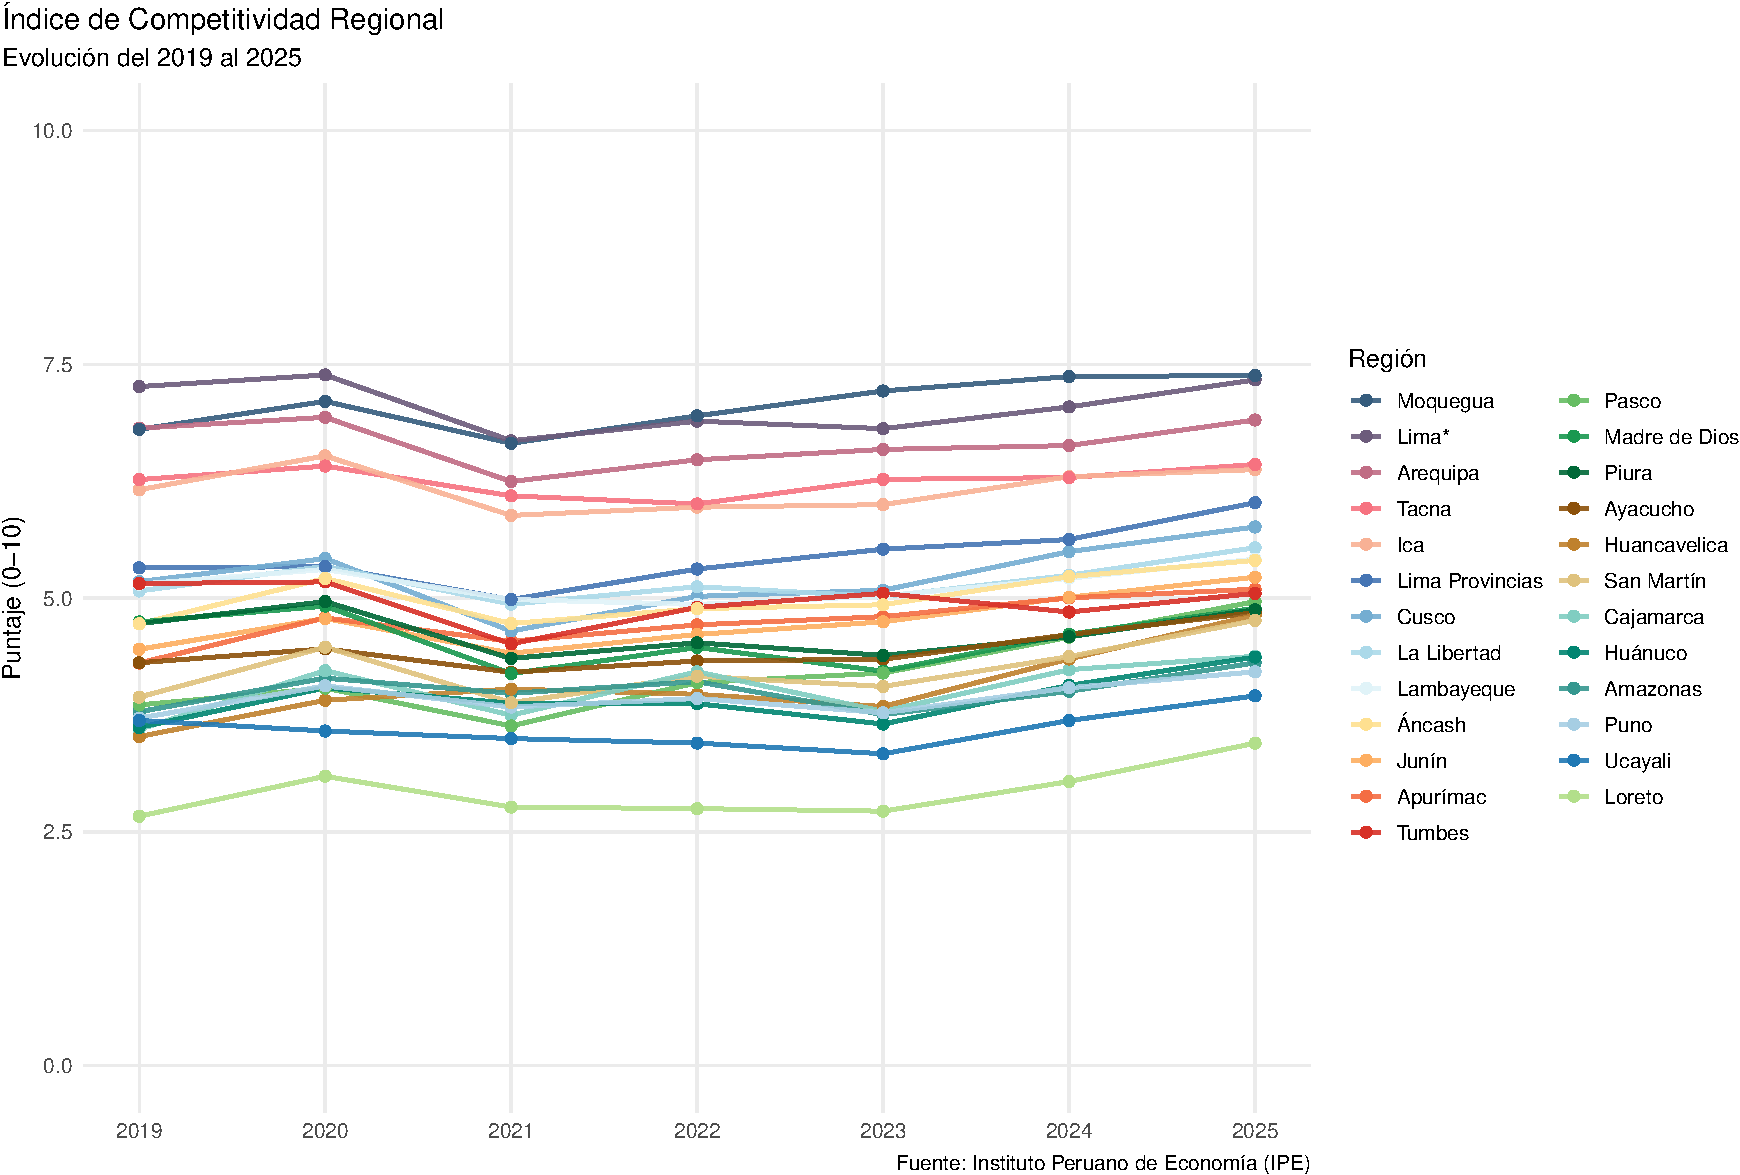
\includegraphics{Manual_files/figure-pdf/unnamed-chunk-36-1.pdf}

\textbf{Resultado esperado.} Una línea por región (índice general),
escala 0--10, puntos visibles y \textbf{orden en leyenda} acorde a la
\textbf{última edición}.

\paragraph{\texorpdfstring{\textbf{2)Pilares con facetado completo y
paleta
accesible}}{2)Pilares con facetado completo y paleta accesible}}\label{pilares-con-facetado-completo-y-paleta-accesible}

\textbf{Se desea lo siguiente:} observar trayectorias por pilar (los
seis paneles)

\begin{Shaded}
\begin{Highlighting}[]
\NormalTok{e2 }\OtherTok{\textless{}{-}} \FunctionTok{general\_largo}\NormalTok{(}
  \AttributeTok{ediciones =} \DecValTok{2020}\SpecialCharTok{:}\DecValTok{2025}\NormalTok{,}
  \AttributeTok{regiones  =} \FunctionTok{c}\NormalTok{(}\StringTok{"gr\_selva"}\NormalTok{),}
  \AttributeTok{modo      =} \StringTok{"pilares"}\NormalTok{,}
  \AttributeTok{paleta    =} \StringTok{"okabe\_ito"}\NormalTok{,}
  \AttributeTok{mostrar\_puntos =} \ConstantTok{TRUE}
\NormalTok{)}
\NormalTok{e2}
\end{Highlighting}
\end{Shaded}

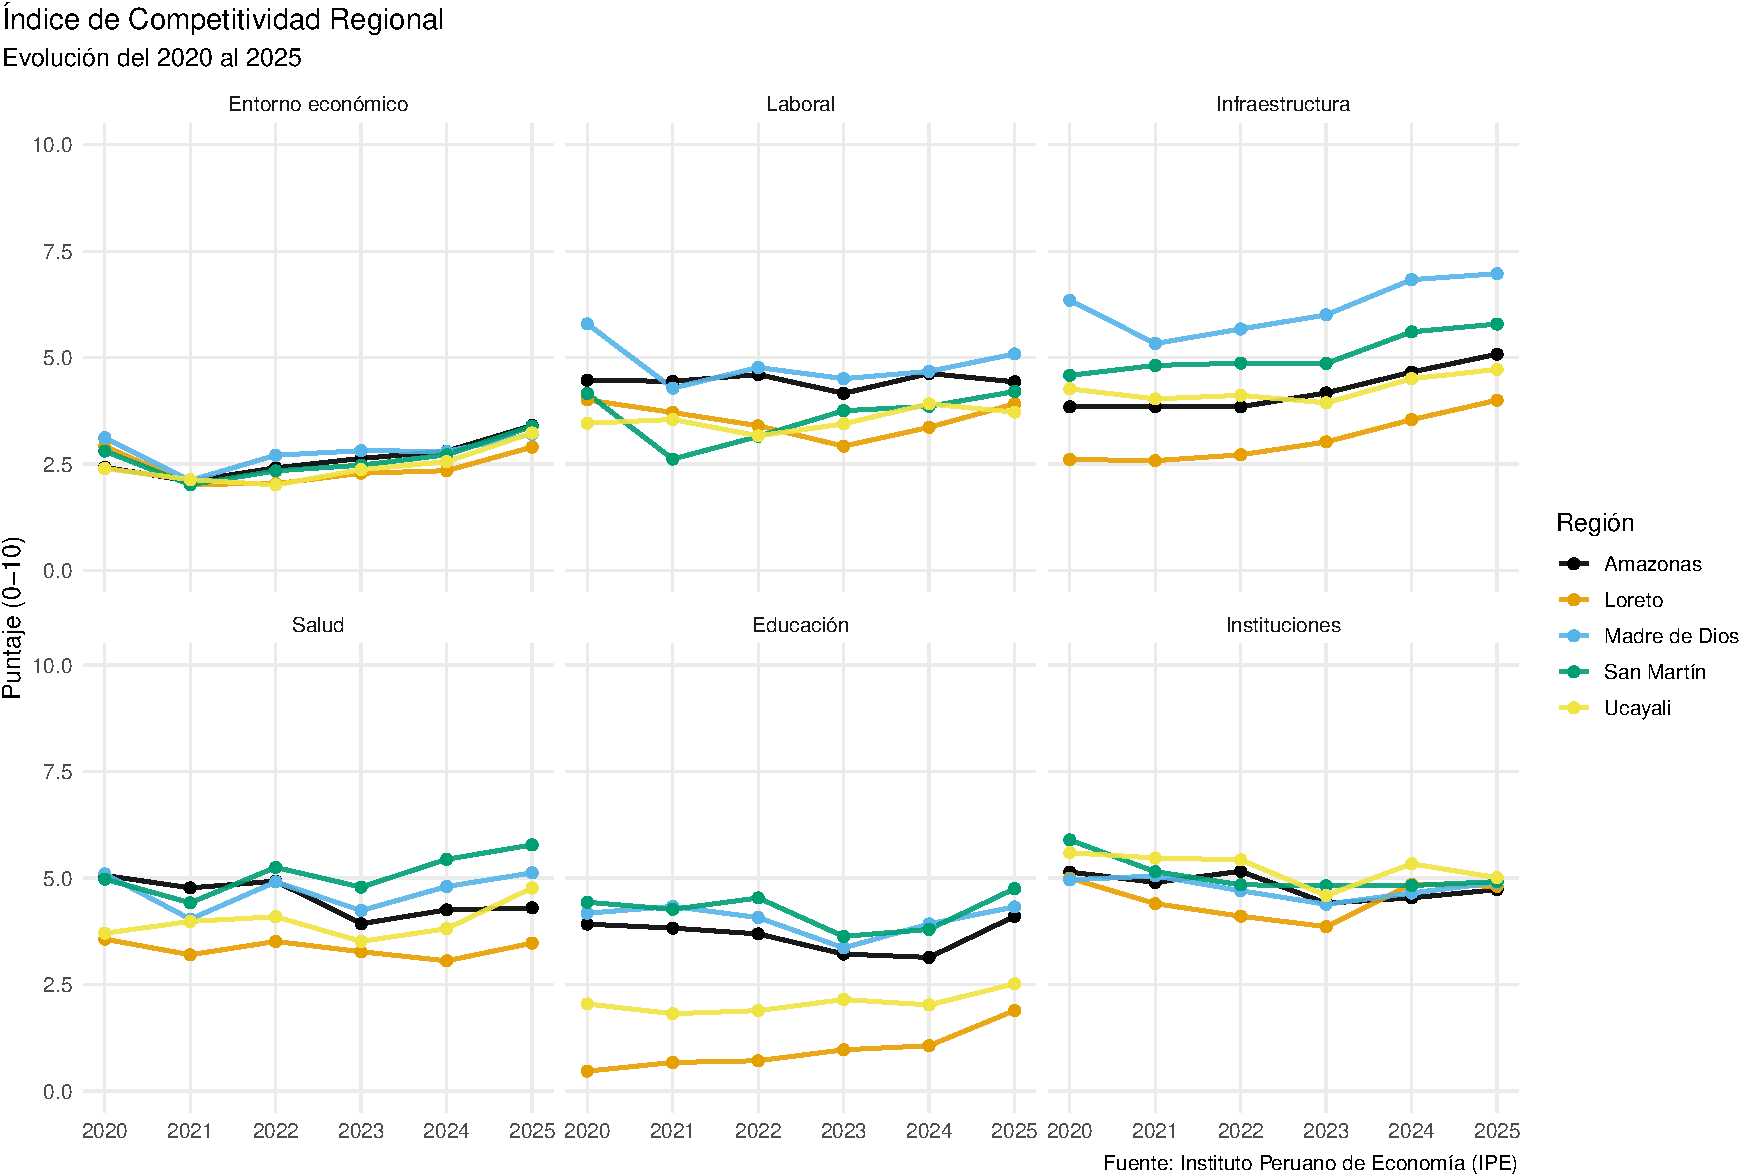
\includegraphics{Manual_files/figure-pdf/unnamed-chunk-37-1.pdf}

\textbf{Resultado esperado.} Seis paneles (pilares), una línea por
región en cada panel.

\paragraph{\texorpdfstring{\textbf{3) Subconjunto territorial con grupo
y
exclusión}}{3) Subconjunto territorial con grupo y exclusión}}\label{subconjunto-territorial-con-grupo-y-exclusiuxf3n}

\textbf{Se desea lo siguiente:} comparar la evolución del índice general
solo para la \textbf{costa}, \textbf{excluyendo Lima}*, con una paleta
perceptual robusta.

\begin{Shaded}
\begin{Highlighting}[]
\NormalTok{e3 }\OtherTok{\textless{}{-}} \FunctionTok{general\_largo}\NormalTok{(}
  \AttributeTok{ediciones =} \DecValTok{2016}\SpecialCharTok{:}\DecValTok{2025}\NormalTok{,}
  \AttributeTok{regiones  =} \FunctionTok{c}\NormalTok{(}\StringTok{"gr\_costa"}\NormalTok{, }\StringTok{"{-}Lima*"}\NormalTok{),}
  \AttributeTok{modo      =} \StringTok{"general"}\NormalTok{,}
  \AttributeTok{paleta    =} \StringTok{"viridis"}\NormalTok{,}
  \AttributeTok{mostrar\_puntos =} \ConstantTok{FALSE}
\NormalTok{)}
\NormalTok{e3}
\end{Highlighting}
\end{Shaded}

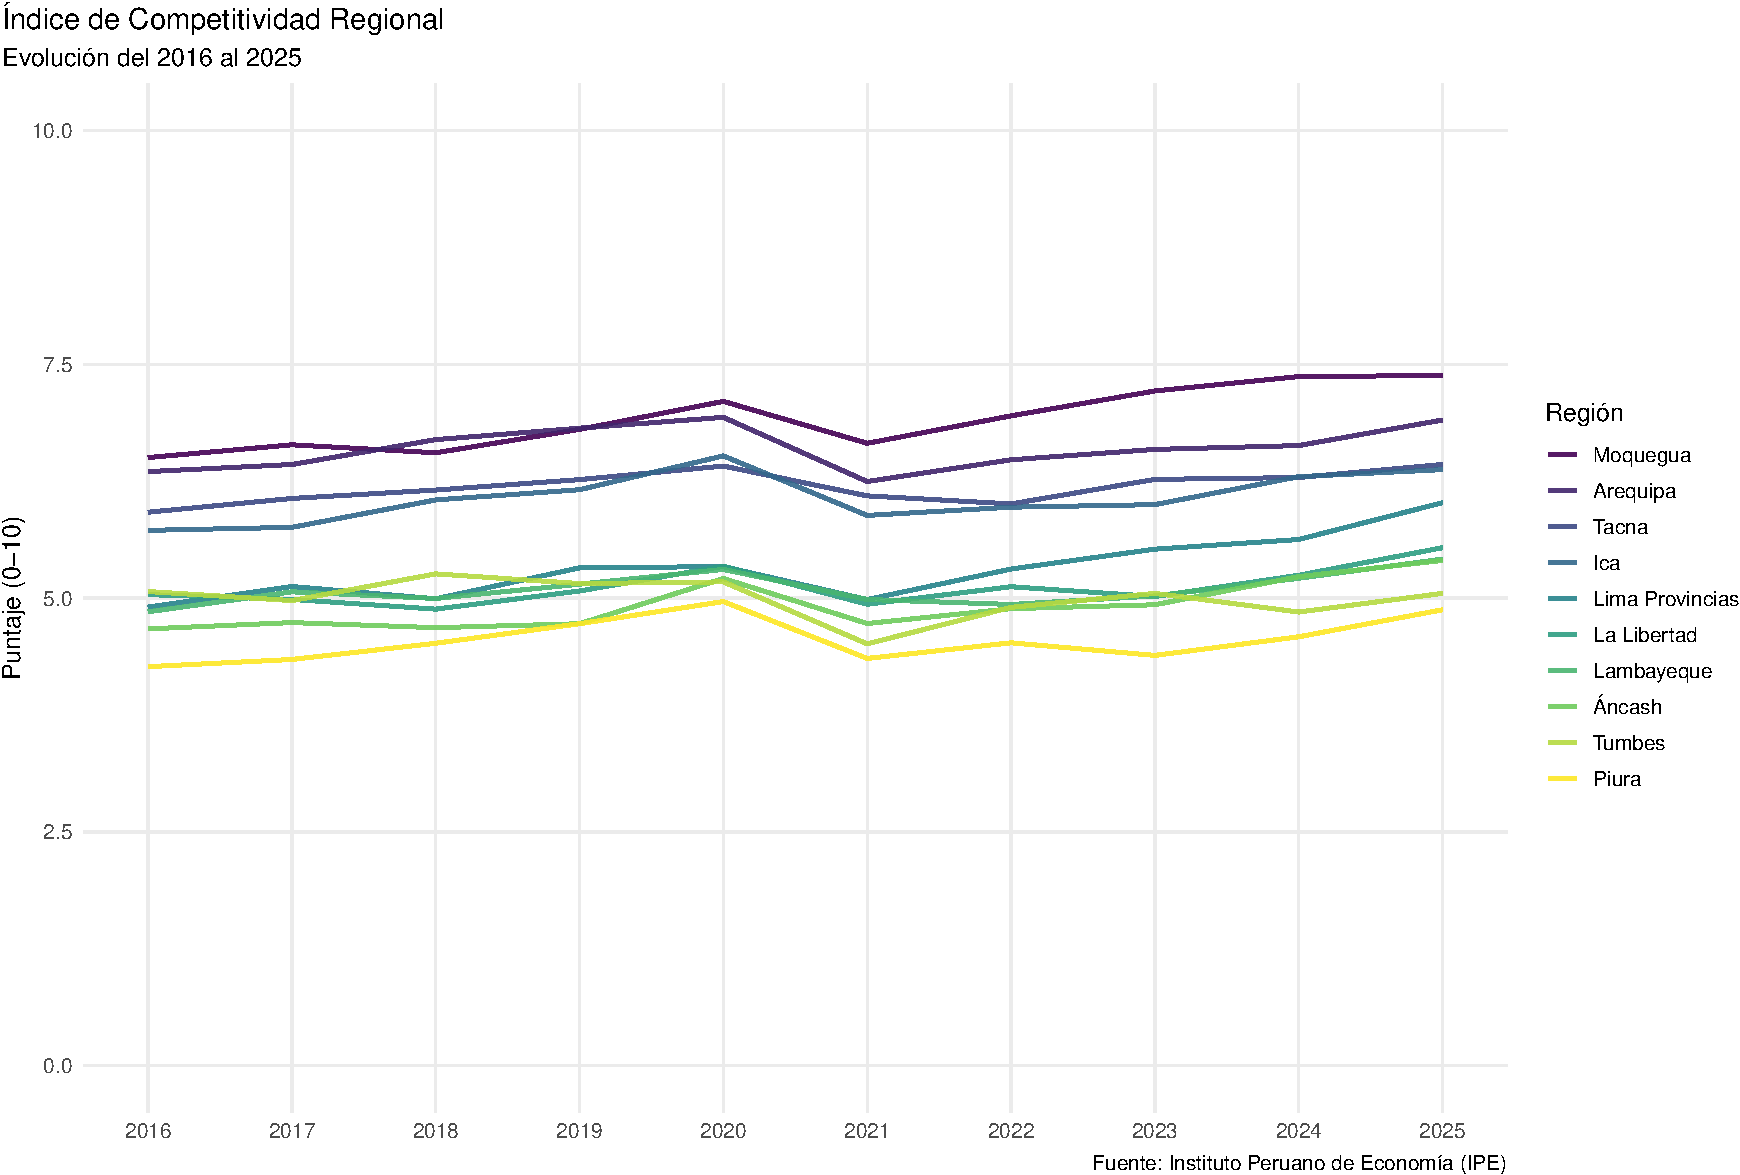
\includegraphics{Manual_files/figure-pdf/unnamed-chunk-38-1.pdf}

\textbf{Resultado esperado.} Líneas más claras en el subconjunto costero
sin Lima*, con \textbf{trazos limpios} (sin puntos) para enfatizar
tendencia.

\paragraph{\texorpdfstring{\textbf{4)Pilares seleccionados mezclando
nombres y
códigos}}{4)Pilares seleccionados mezclando nombres y códigos}}\label{pilares-seleccionados-mezclando-nombres-y-cuxf3digos}

\textbf{Se desea lo siguiente:} analizar solo \textbf{Salud},
\textbf{Infraestructura} y \textbf{Educación} combinando nombres y
códigos de pilar.

\begin{Shaded}
\begin{Highlighting}[]
\NormalTok{e4 }\OtherTok{\textless{}{-}} \FunctionTok{general\_largo}\NormalTok{(}
  \AttributeTok{ediciones =} \DecValTok{2020}\SpecialCharTok{:}\DecValTok{2025}\NormalTok{,}
  \AttributeTok{regiones  =} \FunctionTok{c}\NormalTok{(}\StringTok{"gr\_costa"}\NormalTok{, }\StringTok{"{-}Lima*"}\NormalTok{),}
  \AttributeTok{modo      =} \StringTok{"pilares"}\NormalTok{,}
  \AttributeTok{pilares   =} \FunctionTok{c}\NormalTok{(}\StringTok{"SAL"}\NormalTok{, }\StringTok{"Infraestructura"}\NormalTok{, }\StringTok{"EDU"}\NormalTok{),}
  \AttributeTok{paleta    =} \StringTok{"ipe"}\NormalTok{,}
  \AttributeTok{mostrar\_puntos =} \ConstantTok{TRUE}
\NormalTok{)}
\NormalTok{e4}
\end{Highlighting}
\end{Shaded}

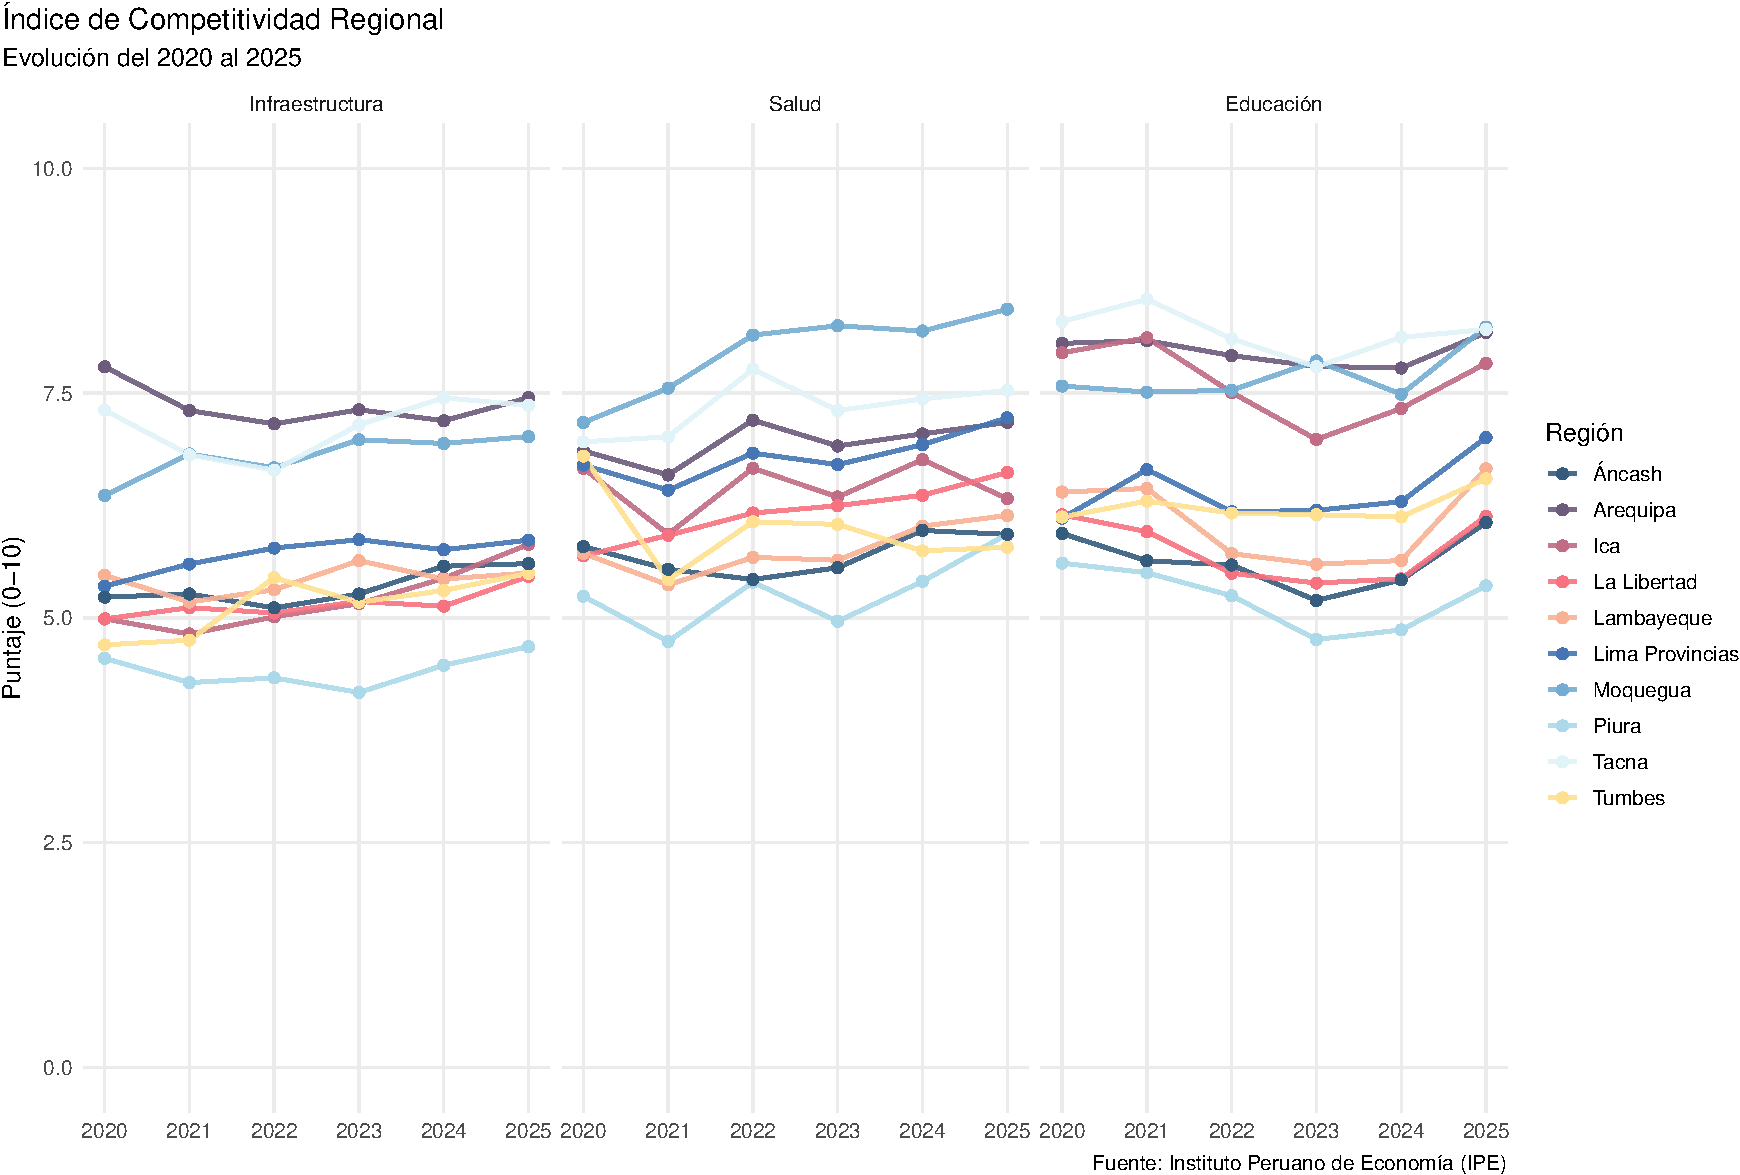
\includegraphics{Manual_files/figure-pdf/unnamed-chunk-39-1.pdf}

\textbf{Resultado esperado.} Facetado con \textbf{tres paneles} (Salud,
Infraestructura, Educación), respetando el color por región e
identificando \textbf{contrastes} en la dinámica por dimensión.

\paragraph{\texorpdfstring{\textbf{5) Serie discontinua y bloque mixto
de
regiones}}{5) Serie discontinua y bloque mixto de regiones}}\label{serie-discontinua-y-bloque-mixto-de-regiones}

\textbf{Se desea lo siguiente:} estudiar un patrón \textbf{no anual}
(ediciones alternas) y centrarse en un \textbf{bloque mixto} de
regiones.

\begin{Shaded}
\begin{Highlighting}[]
\NormalTok{e5 }\OtherTok{\textless{}{-}} \FunctionTok{general\_largo}\NormalTok{(}
  \AttributeTok{ediciones =} \FunctionTok{c}\NormalTok{(}\DecValTok{2016}\NormalTok{, }\DecValTok{2018}\NormalTok{, }\DecValTok{2020}\NormalTok{, }\DecValTok{2022}\NormalTok{, }\DecValTok{2024}\NormalTok{),}
  \AttributeTok{regiones  =} \FunctionTok{c}\NormalTok{(}\StringTok{"gr\_sierra"}\NormalTok{, }\StringTok{"Arequipa"}\NormalTok{, }\StringTok{"La Libertad"}\NormalTok{),}
  \AttributeTok{modo      =} \StringTok{"general"}\NormalTok{,}
  \AttributeTok{paleta    =} \StringTok{"okabe\_ito"}\NormalTok{,}
  \AttributeTok{mostrar\_puntos =} \ConstantTok{TRUE}
\NormalTok{)}
\NormalTok{e5}
\end{Highlighting}
\end{Shaded}

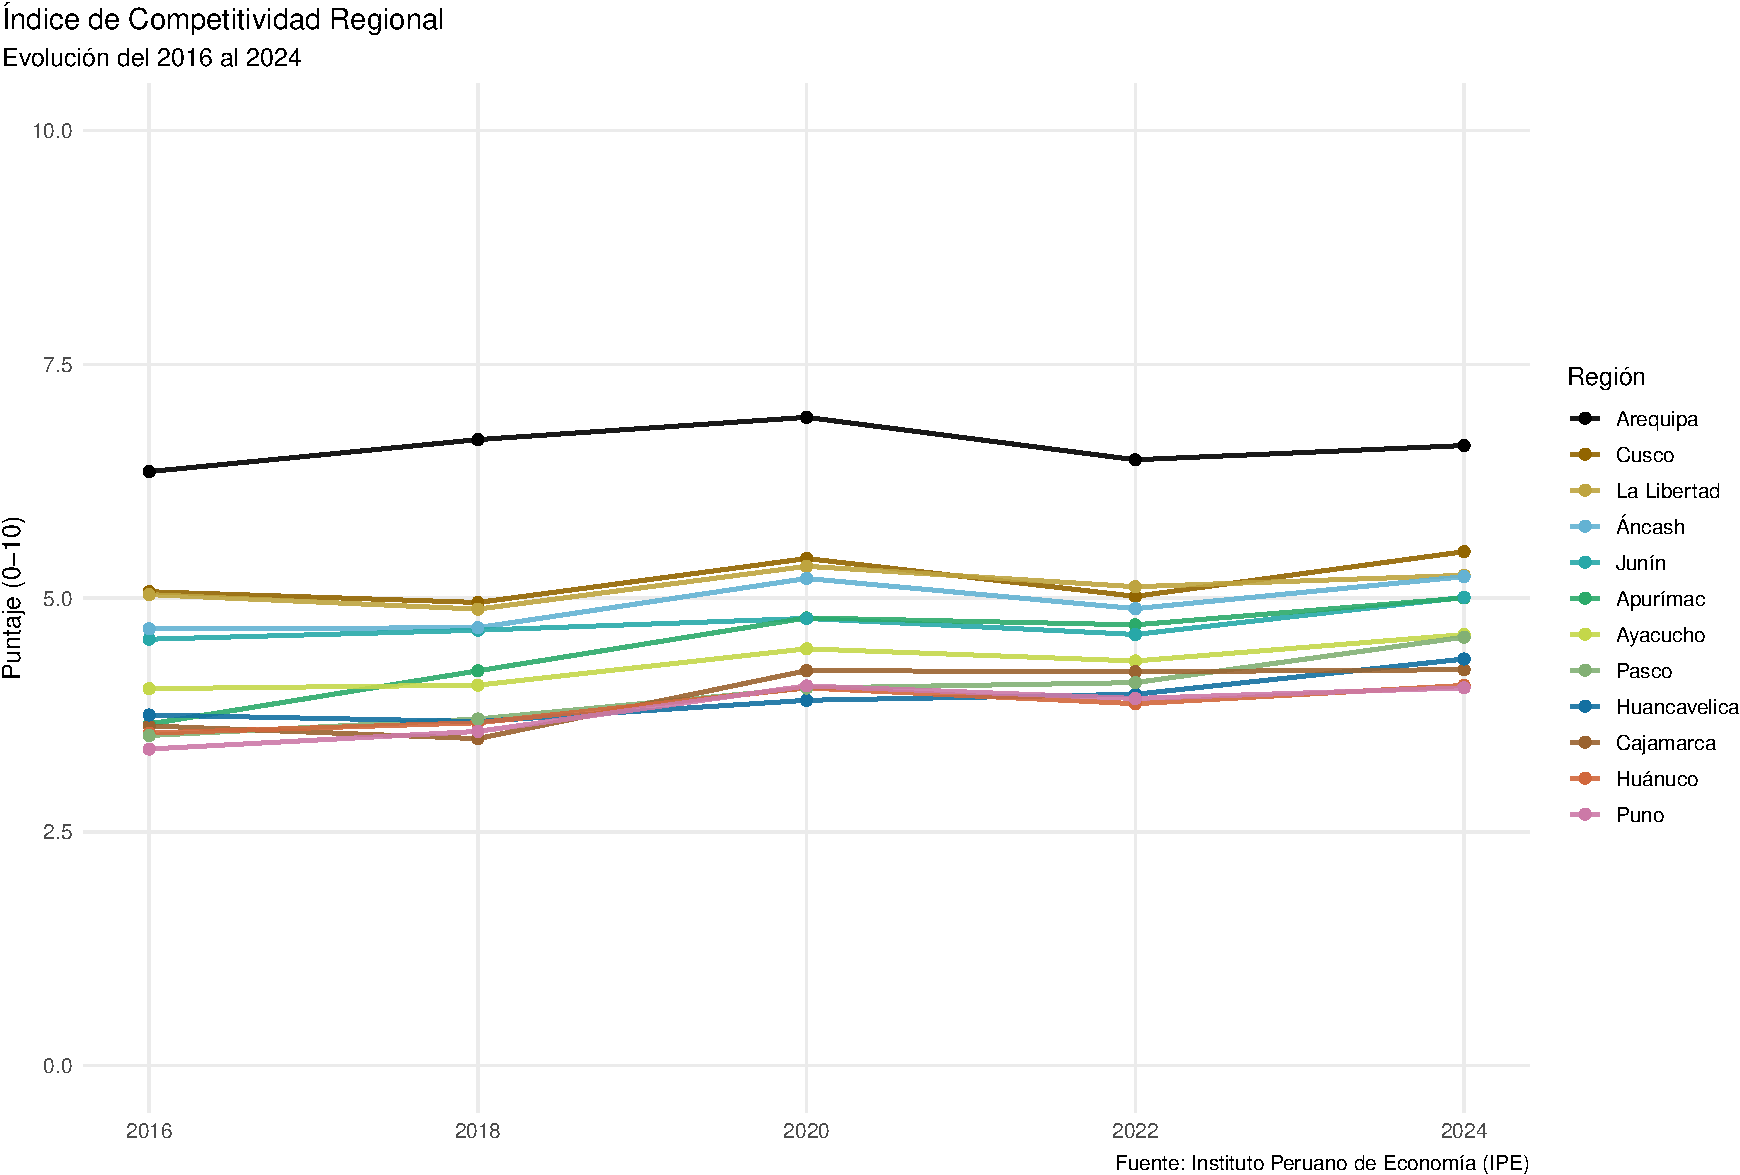
\includegraphics{Manual_files/figure-pdf/unnamed-chunk-40-1.pdf}

\textbf{Resultado esperado.} Evolución en \textbf{años alternos} para un
conjunto formado por \textbf{grupo} + \textbf{regiones puntuales}, los
puntos facilitan comparar niveles en las ediciones muestreadas.

Perfecto. Aquí tienes el texto \textbf{detallado, narrativo y didáctico}
para tu manual sobre \textbf{general\_mapa()}, con los
\textbf{parámetros clave en viñetas} (todas las opciones y valores
envueltos en ``) y \textbf{5 ejemplos} claros que exploran
funcionalidades propias del paquete (grupos gr\_*, exclusiones con
`''-''\,`, zoom a subconjuntos, etiquetas y paletas
continuas/divergentes). Mantengo `usar\_codigos` como argumento
secundario.

\subsection{\texorpdfstring{\textbf{general\_mapa()}}{general\_mapa()}}\label{general_mapa}

\textbf{Mapa coroplético del puntaje General por región (una edición)}

\subsubsection{\texorpdfstring{\textbf{Introducción}}{Introducción}}\label{introducciuxf3n-7}

general\_mapa() resuelve la necesidad de \textbf{ubicar espacialmente}
los resultados del \textbf{Índice de Competitividad Regional (INCORE)}
en \textbf{una edición} específica. A diferencia de un ranking o una
dispersión, el coroplético prioriza la \textbf{lectura territorial}:
permite reconocer \textbf{patrones geográficos} (continuidades,
gradientes, contrastes) y detectar \textbf{bolsones de alto o bajo
desempeño}. La función colorea cada región según su \textbf{puntaje
General (0--10)} y utiliza exclusivamente filas cuyo pilar
\textbf{comienza con} ``Índice de Competitividad Regional'',
garantizando que se represente el \textbf{índice general} y no un pilar.
El subtítulo fija el contexto temporal con ``Puntaje General (YYYY)'',
reforzando la idea de \textbf{corte temporal}.

Se debe cargar primero el mapa:

\subsubsection{\texorpdfstring{\textbf{Parámetros}}{Parámetros}}\label{paruxe1metros-6}

El uso práctico combina tres decisiones: (i) \textbf{qué edición} se
desea mostrar, (ii) \textbf{qué regiones} incluir (todas o un
subconjunto, con soporte a \textbf{grupos} y \textbf{exclusiones}), y
(iii) \textbf{cómo} presentar la figura (paleta, etiquetas, y
\textbf{zoom} opcional sobre un subconjunto). Si no se proporciona un
objeto espacial, la función construye uno adecuado para el Perú.

\begin{itemize}
\item
  \textbf{edicion}: fija la \textbf{edición (año)} a representar, debe
  ser un único valor numérico.

  Opciones y formato:

  \begin{itemize}
  \item
    integer(1)
  \item
    2016 \ldots{} 2025
  \end{itemize}
\item
  \textbf{regiones}: delimita el \textbf{universo de regiones}, admite
  nombres, códigos, \textbf{grupos gr\_*} e
  \textbf{inclusiones/exclusiones} por patrón.

  Opciones y formato:

  \begin{itemize}
  \item
    ``ALL'' (todas las regiones)
  \item
    c(``REGION1'', ``REGION2'')
  \item
    c(``COD1'', ``COD2'')
  \item
    c(``gr\_costa'', ``gr\_sierra'', ``gr\_selva'')
  \item
    Exclusiones: ``-Lima*''
  \item
    Combinaciones mixtas: c(``gr\_costa'', ``La Libertad'', ``-Lima*'')
  \end{itemize}
\item
  \textbf{mapa\_sf}: objeto espacial con columnas ``region'' y
  ``geometry''.

  Opciones y formato:

  \begin{itemize}
  \item
    NULL (por defecto, se crea con mapa\_peru())
  \item
    sf o SpatVector convertible a sf con st\_as\_sf()
  \end{itemize}
\item
  \textbf{paleta}: controla la \textbf{escala continua} de color
  (0--10).

  Opciones y formato:

  \begin{itemize}
  \item
    ``blues'' (por defecto, progresión fría sobria)
  \item
    ``greens'' (alternativa sobria en verdes)
  \item
    ``viridis'' (perceptualmente uniforme)
  \item
    ``cividis'' (robusta en proyección e impresión)
  \item
    ``divergente'' (bicolor con punto medio en 5, útil para ``por
    encima/por debajo'')
  \end{itemize}
\item
  \textbf{simplificar}: tolerancia de \textbf{simplificación geométrica}
  (al crear mapa\_peru()) para aligerar el dibujo.

  Opciones y formato:

  \begin{itemize}
  \item
    0 (sin simplificar, por defecto)
  \item
    \textgreater{} 0 (mayores valores ⇒ geometrías más simples)
  \end{itemize}
\item
  \textbf{zoom}: decide si \textbf{recortar la vista} al \emph{bounding
  box} del subconjunto \textbf{seleccionado} en regiones.

  Opciones y formato:

  \begin{itemize}
  \item
    FALSE (por defecto, vista nacional)
  \item
    TRUE (activa zoom si regiones ≠ ``ALL'')
  \end{itemize}
\item
  \textbf{expand\_zoom}: margen \textbf{proporcional} alrededor del
  \emph{bounding box} cuando zoom = TRUE.

  Opciones y formato:

  \begin{itemize}
  \item
    0.04 (por defecto)
  \item
    0 \ldots{} 0.2 (aprox., según preferencia de encuadre)
  \end{itemize}
\item
  \textbf{etiquetas}: controla cómo \textbf{anotar los valores} dentro
  de cada región.

  Opciones y formato:

  \begin{itemize}
  \item
    ``repel'' (por defecto, usa ggrepel si está disponible)
  \item
    ``texto'' (etiquetas directas con geom\_text)
  \item
    ``ninguna'' (sin etiquetas internas)
  \end{itemize}
\end{itemize}

El parámetro \textbf{usar\_codigos} es operativo: cuando es TRUE, la
función \textbf{traduce códigos} a nombres oficiales para mantener
consistencia editorial en el mapa y las etiquetas. Mantenerlo activado
suele ser lo más conveniente.

\subsubsection{\texorpdfstring{\textbf{Explicación
conceptual}}{Explicación conceptual}}\label{explicaciuxf3n-conceptual-6}

La función \textbf{lee} la edición solicitada, \textbf{filtra}
únicamente el \textbf{índice general} (excluyendo ``Perú'' para
conservar el foco subnacional) y, si se especificó regiones,
\textbf{expande grupos} gr\_* y \textbf{aplica exclusiones}. Antes de
mapear, \textbf{consolida} un único valor por región (promedio defensivo
y redondeo), y \textbf{une} los datos al objeto espacial. Cuando se
establece un subconjunto, el resto de regiones quedan con \textbf{NA} y
se dibujan en \textbf{gris} para no inducir comparaciones donde no hay
dato mostrado. La \textbf{paleta continua} fija los límites en
\textbf{0--10}, y las \textbf{etiquetas} (si se activan) se colocan
sobre puntos internos de cada polígono, favoreciendo la legibilidad. El
\textbf{zoom opcional} centra la vista en el subconjunto, con un margen
expand\_zoom para evitar recortes visuales.

\subsubsection{\texorpdfstring{\textbf{Ejemplos}}{Ejemplos}}\label{ejemplos-6}

\paragraph{\texorpdfstring{\textbf{1) Mapa nacional básico (paleta por
defecto)}}{1) Mapa nacional básico (paleta por defecto)}}\label{mapa-nacional-buxe1sico-paleta-por-defecto}

\paragraph{\texorpdfstring{\textbf{Se desea lo siguiente:} representar
el \textbf{índice general} en una edición reciente para \textbf{todas}
las
regiones.}{Se desea lo siguiente: representar el índice general en una edición reciente para todas las regiones.}}\label{se-desea-lo-siguiente-representar-el-uxedndice-general-en-una-ediciuxf3n-reciente-para-todas-las-regiones.}

\begin{Shaded}
\begin{Highlighting}[]
\NormalTok{m1 }\OtherTok{\textless{}{-}} \FunctionTok{general\_mapa}\NormalTok{(}
  \AttributeTok{edicion  =} \DecValTok{2025}\NormalTok{,}
  \AttributeTok{regiones =} \StringTok{"ALL"}\NormalTok{,}
  \AttributeTok{paleta   =} \StringTok{"blues"}\NormalTok{,}
  \AttributeTok{etiquetas =} \StringTok{"repel"}
\NormalTok{)}
\NormalTok{m1}
\end{Highlighting}
\end{Shaded}

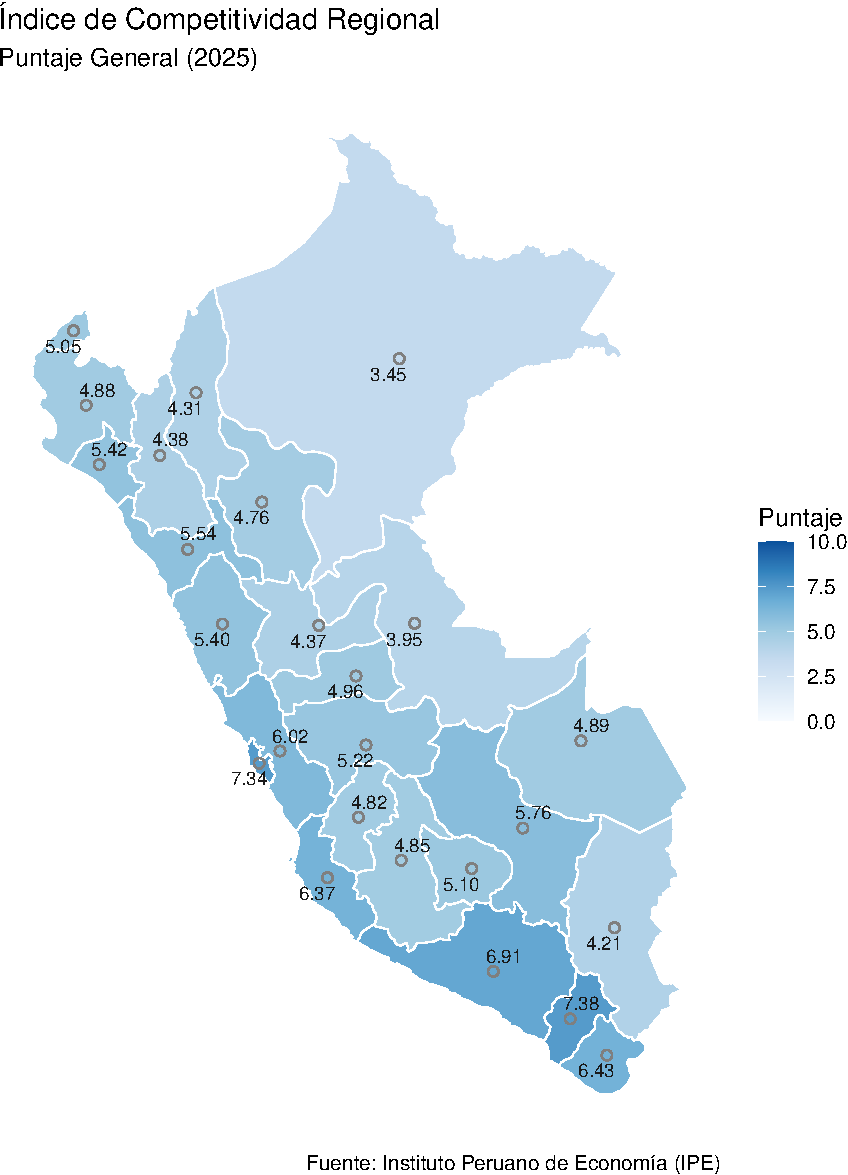
\includegraphics{Manual_files/figure-pdf/unnamed-chunk-42-1.pdf}

\textbf{Resultado esperado.} Coroplético nacional 0--10.

\paragraph{\texorpdfstring{\textbf{2) Subconjunto por grupo con zoom
automático}}{2) Subconjunto por grupo con zoom automático}}\label{subconjunto-por-grupo-con-zoom-automuxe1tico}

\textbf{Se desea lo siguiente:} concentrar la lectura en \textbf{costa},
con recorte automático del encuadre.

\begin{Shaded}
\begin{Highlighting}[]
\NormalTok{m2 }\OtherTok{\textless{}{-}} \FunctionTok{general\_mapa}\NormalTok{(}
  \AttributeTok{edicion   =} \DecValTok{2025}\NormalTok{,}
  \AttributeTok{regiones  =} \FunctionTok{c}\NormalTok{(}\StringTok{"gr\_costa"}\NormalTok{),}
  \AttributeTok{paleta    =} \StringTok{"viridis"}\NormalTok{,}
  \AttributeTok{zoom      =} \ConstantTok{TRUE}\NormalTok{,}
  \AttributeTok{expand\_zoom =} \FloatTok{0.05}\NormalTok{,}
  \AttributeTok{etiquetas =} \StringTok{"repel"}
\NormalTok{)}
\NormalTok{m2}
\end{Highlighting}
\end{Shaded}

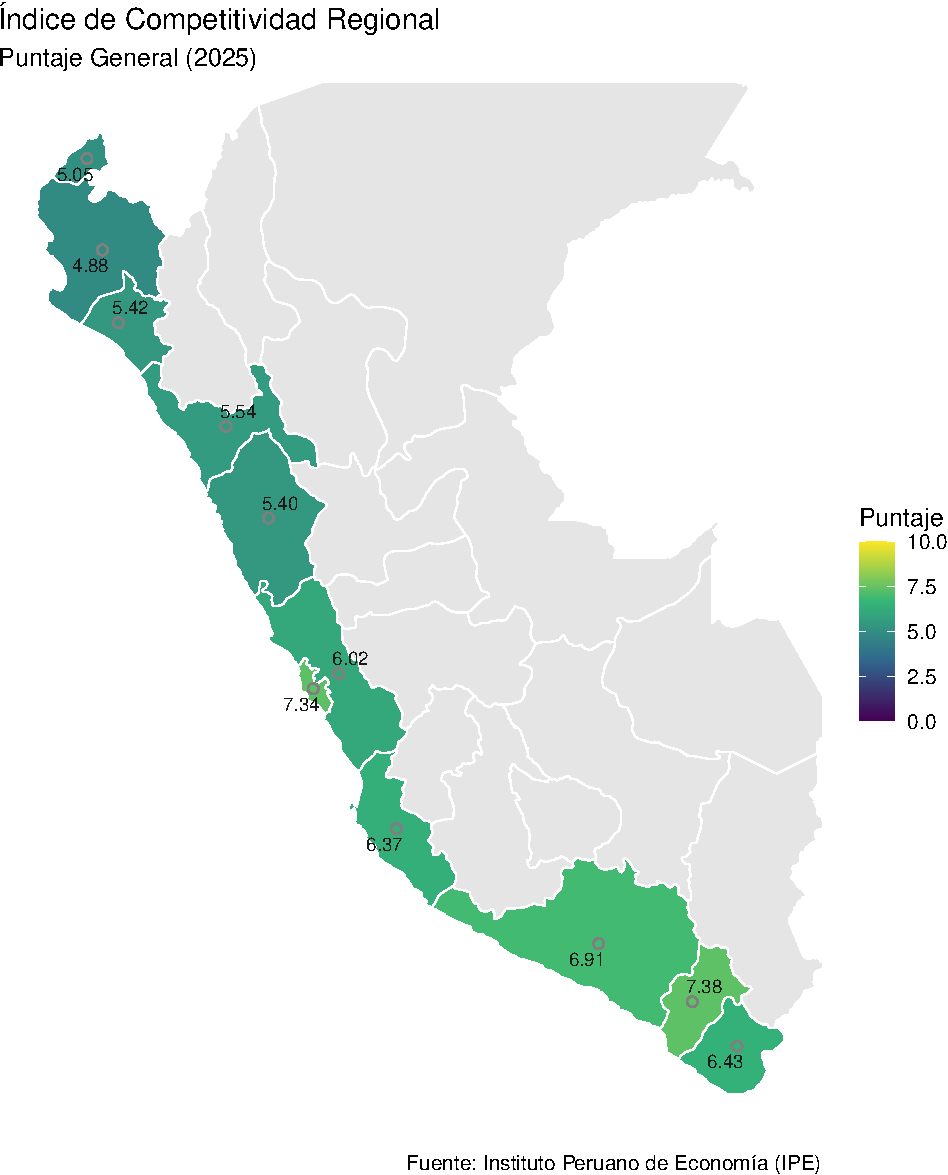
\includegraphics{Manual_files/figure-pdf/unnamed-chunk-43-1.pdf}

\textbf{Resultado esperado.} Vista recortada a la \textbf{costa}, paleta
``viridis'' y etiquetas repel que evitan solapamientos.

\paragraph{\texorpdfstring{\textbf{3) Subconjunto mixto con exclusión y
etiquetas
simples}}{3) Subconjunto mixto con exclusión y etiquetas simples}}\label{subconjunto-mixto-con-exclusiuxf3n-y-etiquetas-simples}

\textbf{Se desea lo siguiente:} mostrar un bloque mixto (grupo +
regiones puntuales) \textbf{excluyendo Lima}* y usar etiquetas simples.

\begin{Shaded}
\begin{Highlighting}[]
\NormalTok{m3 }\OtherTok{\textless{}{-}} \FunctionTok{general\_mapa}\NormalTok{(}
  \AttributeTok{edicion   =} \DecValTok{2025}\NormalTok{,}
  \AttributeTok{regiones  =} \FunctionTok{c}\NormalTok{(}\StringTok{"gr\_sierra"}\NormalTok{, }\StringTok{"Arequipa"}\NormalTok{, }\StringTok{"La Libertad"}\NormalTok{, }\StringTok{"{-}Lima*"}\NormalTok{),}
  \AttributeTok{paleta    =} \StringTok{"cividis"}\NormalTok{,}
  \AttributeTok{zoom      =} \ConstantTok{TRUE}\NormalTok{,}
  \AttributeTok{etiquetas =} \StringTok{"texto"}
\NormalTok{)}
\NormalTok{m3}
\end{Highlighting}
\end{Shaded}

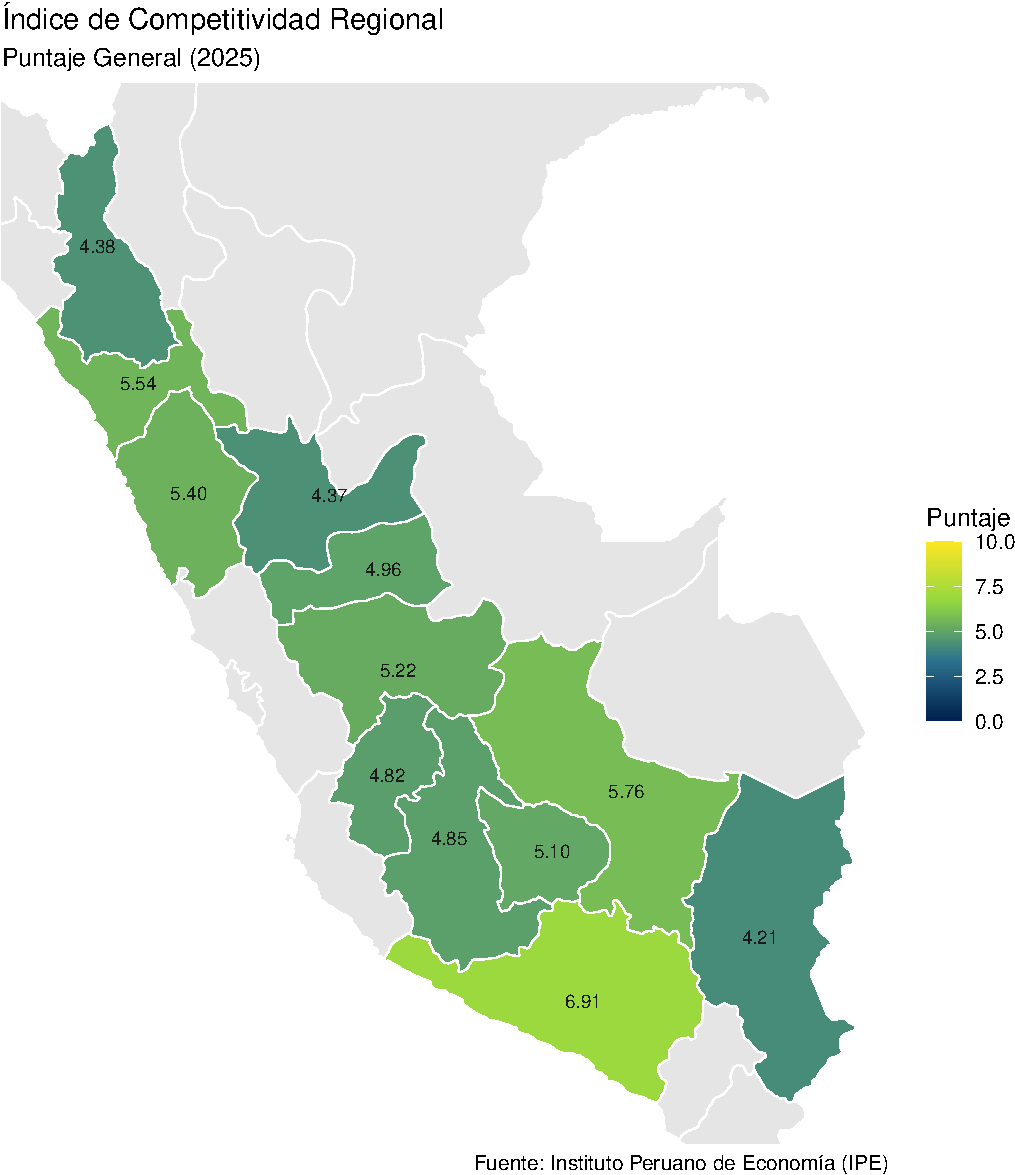
\includegraphics{Manual_files/figure-pdf/unnamed-chunk-44-1.pdf}

\textbf{Resultado esperado.} Coroplético del subconjunto, \textbf{sin
Lima}*, con etiquetas directas y encuadre ajustado al bloque.

\paragraph{\texorpdfstring{\textbf{4) Paleta divergente para lectura
``por encima / por
debajo''}}{4) Paleta divergente para lectura ``por encima / por debajo''}}\label{paleta-divergente-para-lectura-por-encima-por-debajo}

\textbf{Se desea lo siguiente:} enfatizar si las regiones están por
\textbf{encima} o \textbf{debajo} de un punto medio (5).

\begin{Shaded}
\begin{Highlighting}[]
\NormalTok{m4 }\OtherTok{\textless{}{-}} \FunctionTok{general\_mapa}\NormalTok{(}
  \AttributeTok{edicion   =} \DecValTok{2025}\NormalTok{,}
  \AttributeTok{regiones  =} \StringTok{"ALL"}\NormalTok{,}
  \AttributeTok{paleta    =} \StringTok{"divergente"}\NormalTok{,}
  \AttributeTok{etiquetas =} \StringTok{"ninguna"}
\NormalTok{)}
\NormalTok{m4}
\end{Highlighting}
\end{Shaded}

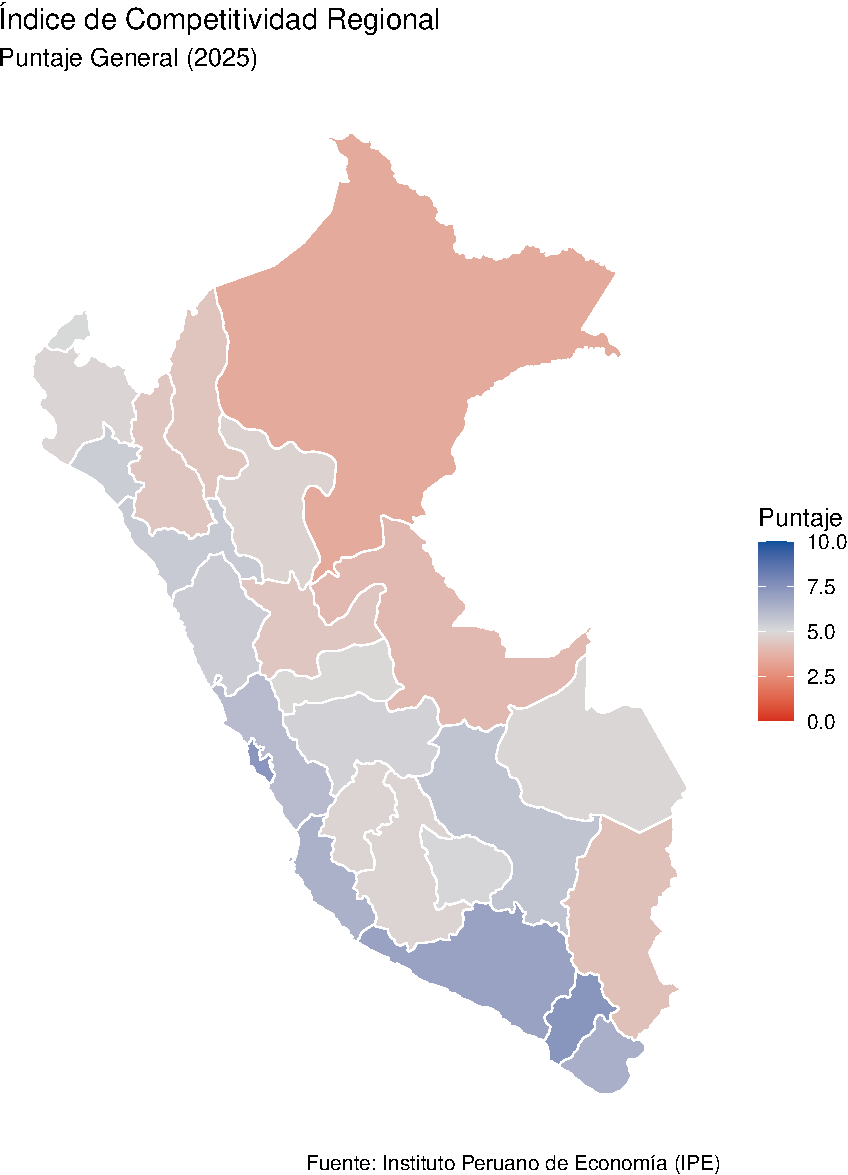
\includegraphics{Manual_files/figure-pdf/unnamed-chunk-45-1.pdf}

\textbf{Resultado esperado.} Paleta bicolor con \textbf{midpoint = 5}:
útil para lecturas rápidas tipo ``alto/bajo'' respecto de un umbral
simbólico.

\paragraph{\texorpdfstring{\textbf{5) Mapa ligero para informes:
simplificación
geométrica}}{5) Mapa ligero para informes: simplificación geométrica}}\label{mapa-ligero-para-informes-simplificaciuxf3n-geomuxe9trica}

\textbf{Se desea lo siguiente:} mapa de la región sur

\begin{Shaded}
\begin{Highlighting}[]
\NormalTok{m5 }\OtherTok{\textless{}{-}} \FunctionTok{general\_mapa}\NormalTok{(}
  \AttributeTok{edicion     =} \DecValTok{2025}\NormalTok{,}
  \AttributeTok{regiones    =} \StringTok{"gr\_sur"}\NormalTok{,}
  \AttributeTok{paleta      =} \StringTok{"greens"}\NormalTok{,}
  \AttributeTok{simplificar =} \FloatTok{0.02}\NormalTok{,}
  \AttributeTok{etiquetas   =} \StringTok{"repel"}\NormalTok{,}
  \AttributeTok{zoom =}\NormalTok{ T}
\NormalTok{)}
\NormalTok{m5}
\end{Highlighting}
\end{Shaded}

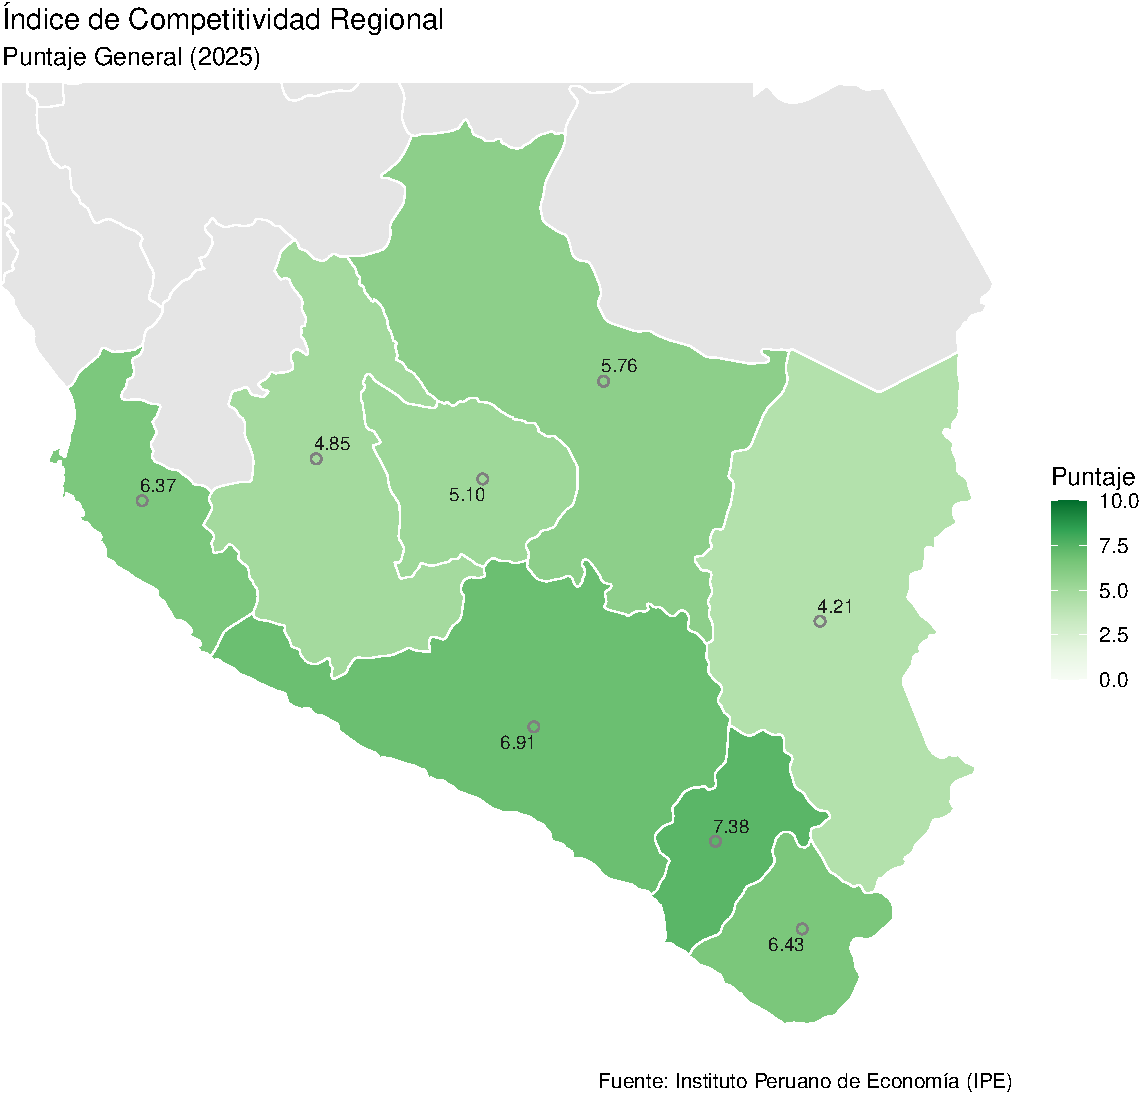
\includegraphics{Manual_files/figure-pdf/unnamed-chunk-46-1.pdf}

\subsection{\texorpdfstring{\textbf{general\_media()}}{general\_media()}}\label{general_media}

\textbf{Dispersión del puntaje General (total o de un pilar) frente a un
promedio}

Su foco es mostrar, en \textbf{una edición} del INCORE, cómo se sitúan
las \textbf{regiones} frente a un \textbf{promedio de referencia}. El
gráfico representa, en el eje \textbf{X}, el \textbf{puntaje General
(0--10)} y, en el eje \textbf{Y}, las \textbf{regiones}. Cada región
incluye: (i) una \textbf{línea} que va desde el \textbf{promedio} hasta
su valor y (ii) un \textbf{punto} en el valor observado, más una
\textbf{etiqueta} numérica. La referencia central puede ser el
\textbf{promedio nacional} (todas las regiones) o el \textbf{promedio de
la selección} (solo las regiones filtradas para el gráfico).

\subsubsection{\texorpdfstring{\textbf{Introducción}}{Introducción}}\label{introducciuxf3n-8}

general\_media() resuelve un problema recurrente en la comunicación de
resultados: \textbf{ubicar a cada región respecto de un promedio} de
referencia. Mientras un ranking ordena, este diseño enfatiza la
\textbf{distancia a la media} (y su dirección), permitiendo responder
preguntas como: ¿qué regiones están \textbf{por encima} del promedio y
cuáles \textbf{por debajo}?, ¿cuán lejos se encuentran?, ¿existe un
bloque de regiones en torno al promedio? La función admite trabajar con
el \textbf{índice general total} o con el \textbf{General de un pilar}
específico, y ofrece \textbf{cinco esquemas de color} que refuerzan
diferentes lecturas (binaria, continua divergente, bandas tipo
``semáforo'', color por región, o monocromo).

\subsubsection{\texorpdfstring{\textbf{Parámetros}}{Parámetros}}\label{paruxe1metros-7}

La práctica con general\_media() descansa en tres decisiones: (i)
\textbf{qué se grafica} (general total vs.~un pilar), (ii) \textbf{qué
universo regional} se considera (todas o un subconjunto) y (iii)
\textbf{qué promedio} funge como referente (nacional vs.~selección).
Sobre eso, se elige el \textbf{esquema de color} que mejor sirva el
mensaje.

\begin{itemize}
\item
  \textbf{edicion}: fija la \textbf{edición (año)} a graficar, un único
  valor numérico.

  Opciones y formato:

  \begin{itemize}
  \item
    integer(1)
  \item
    2016 \ldots{} 2025
  \end{itemize}
\item
  \textbf{pilar}: determina el \textbf{contenido} a graficar:
  \textbf{índice general total} o \textbf{General de un pilar}.

  Opciones y formato:

  \begin{itemize}
  \item
    NULL (por defecto, índice general total, filas cuyo pilar inicia con
    ``Índice de Competitividad Regional'')
  \item
    Nombre de pilar: ``Salud'', ``Educación'', ``Infraestructura'', etc.
  \item
    Código de pilar: ``SAL'', ``EDU'', ``INF'', etc.
  \end{itemize}
\item
  \textbf{regiones}: delimita el \textbf{universo de regiones} a
  representar, admite nombres, códigos, \textbf{grupos gr\_*} e
  \textbf{inclusiones/exclusiones} por patrón.

  Opciones y formato:

  \begin{itemize}
  \item
    ``ALL'' (todas las regiones)
  \item
    c(``REGION1'', ``REGION2'')
  \item
    c(``COD1'', ``COD2'')
  \item
    c(``gr\_costa'', ``gr\_sierra'', ``gr\_selva'')
  \item
    Exclusiones: ``-Lima*''
  \item
    Mezcla: c(``gr\_costa'', ``La Libertad'', ``-Lima*'')
  \end{itemize}
\item
  \textbf{promedio\_nacional}: define el \textbf{promedio de
  referencia}.

  Opciones y formato:

  \begin{itemize}
  \item
    FALSE (por defecto, promedio sobre la \textbf{selección filtrada})
  \item
    TRUE (promedio \textbf{nacional} calculado sobre \textbf{todas} las
    regiones disponibles en la edición)
  \end{itemize}
\item
  \textbf{esquema}: elige el \textbf{enfoque cromático} del gráfico.

  Opciones y formato:

  \begin{itemize}
  \item
    ``binario'': dos colores según valor \textgreater= promedio
    vs.~\textless{} promedio
  \item
    ``divergente'': gradiente centrado en 0 sobre la diferencia valor -
    promedio
  \item
    ``semaforo'': tres bandas (bajo, en torno, alto) con tolerancia
    interna
  \item
    ``region'': color \textbf{por región} (paletas cualitativas)
  \item
    ``monocromo'': un solo color para todo el trazo/punto
  \end{itemize}
\item
  \textbf{color\_arriba}, \textbf{color\_abajo}: colores para
  ``binario'' (y extremos en ``divergente'').

  Opciones y formato:

  \begin{itemize}
  \item
    color\_arriba = ``\#\#2C7FB8'', color\_abajo = ``\#\#D7301F'' (por
    defecto)
  \item
    Cualquier color válido en R (hex, nombre, etc.)
  \end{itemize}
\item
  \textbf{paleta\_region} \emph{(cuando esquema = ``region'')}: paleta
  cualitativa para \textbf{regiones}.

  Opciones y formato:

  \begin{itemize}
  \item
    ``ipe'' (por defecto)
  \item
    ``okabe\_ito''
  \item
    ``viridis''
  \end{itemize}
\item
  \textbf{color\_mono} \emph{(cuando esquema = ``monocromo'')}: color
  único para segmentos y puntos.

  Opciones y formato:

  \begin{itemize}
  \item
    ``\#\#3B5B92'' (por defecto)
  \item
    Cualquier color válido
  \end{itemize}
\item
  \textbf{mostrar\_leyenda}: controla si se muestra \textbf{leyenda}.

  Opciones y formato:

  \begin{itemize}
  \item
    FALSE (por defecto)
  \item
    TRUE (relevante sobre todo para ``binario'', ``divergente'',
    ``semaforo'' y ``region'')
  \end{itemize}
\end{itemize}

\subsubsection{\texorpdfstring{\textbf{Explicación
conceptual}}{Explicación conceptual}}\label{explicaciuxf3n-conceptual-7}

La función \textbf{lee} la edición solicitada, \textbf{filtra} a Puntaje
del 0 al 10 y, si se especifica pilar, restringe a indicador ==
``General'' de ese pilar, si pilar = NULL, toma el \textbf{índice
general total}. Para regiones, resuelve \textbf{grupos gr\_*} y
\textbf{exclusiones}. Calcula luego un único valor por región (promedio
defensivo y redondeo) y determina el \textbf{promedio de referencia}:
\textbf{nacional} (si promedio\_nacional = TRUE) o de la
\textbf{selección} filtrada (por defecto).

El gráfico traza una \textbf{línea horizontal} por región, con origen en
el \textbf{promedio} y destino en su \textbf{valor}, y un \textbf{punto}
en el valor. La \textbf{anotación} numérica se desplaza levemente para
evitar solapes y mejorar la legibilidad. La paleta elegida en esquema
guía la lectura: \textbf{comparación binaria}, \textbf{gradiente
divergente}, \textbf{bandas semafóricas}, \textbf{identidad por región}
o \textbf{sobriedad monocroma}.

\subsubsection{\texorpdfstring{\textbf{Ejemplos}}{Ejemplos}}\label{ejemplos-7}

\paragraph{\texorpdfstring{\textbf{1) Índice General con esquema binario
(promedio de la
selección)}}{1) Índice General con esquema binario (promedio de la selección)}}\label{uxedndice-general-con-esquema-binario-promedio-de-la-selecciuxf3n}

\textbf{Se desea lo siguiente:} comparar las regiones frente al
\textbf{promedio de la selección} (todas, porque no se filtra) usando
dos colores.

\begin{Shaded}
\begin{Highlighting}[]
\NormalTok{g1 }\OtherTok{\textless{}{-}} \FunctionTok{general\_media}\NormalTok{(}
  \AttributeTok{edicion =} \DecValTok{2025}\NormalTok{,}
  \AttributeTok{pilar   =} \ConstantTok{NULL}\NormalTok{,          }\DocumentationTok{\#\# índice general total}
  \AttributeTok{regiones =} \StringTok{"ALL"}\NormalTok{,}
  \AttributeTok{esquema =} \StringTok{"binario"}\NormalTok{,}
  \AttributeTok{mostrar\_leyenda =} \ConstantTok{TRUE}
\NormalTok{)}
\NormalTok{g1}
\end{Highlighting}
\end{Shaded}

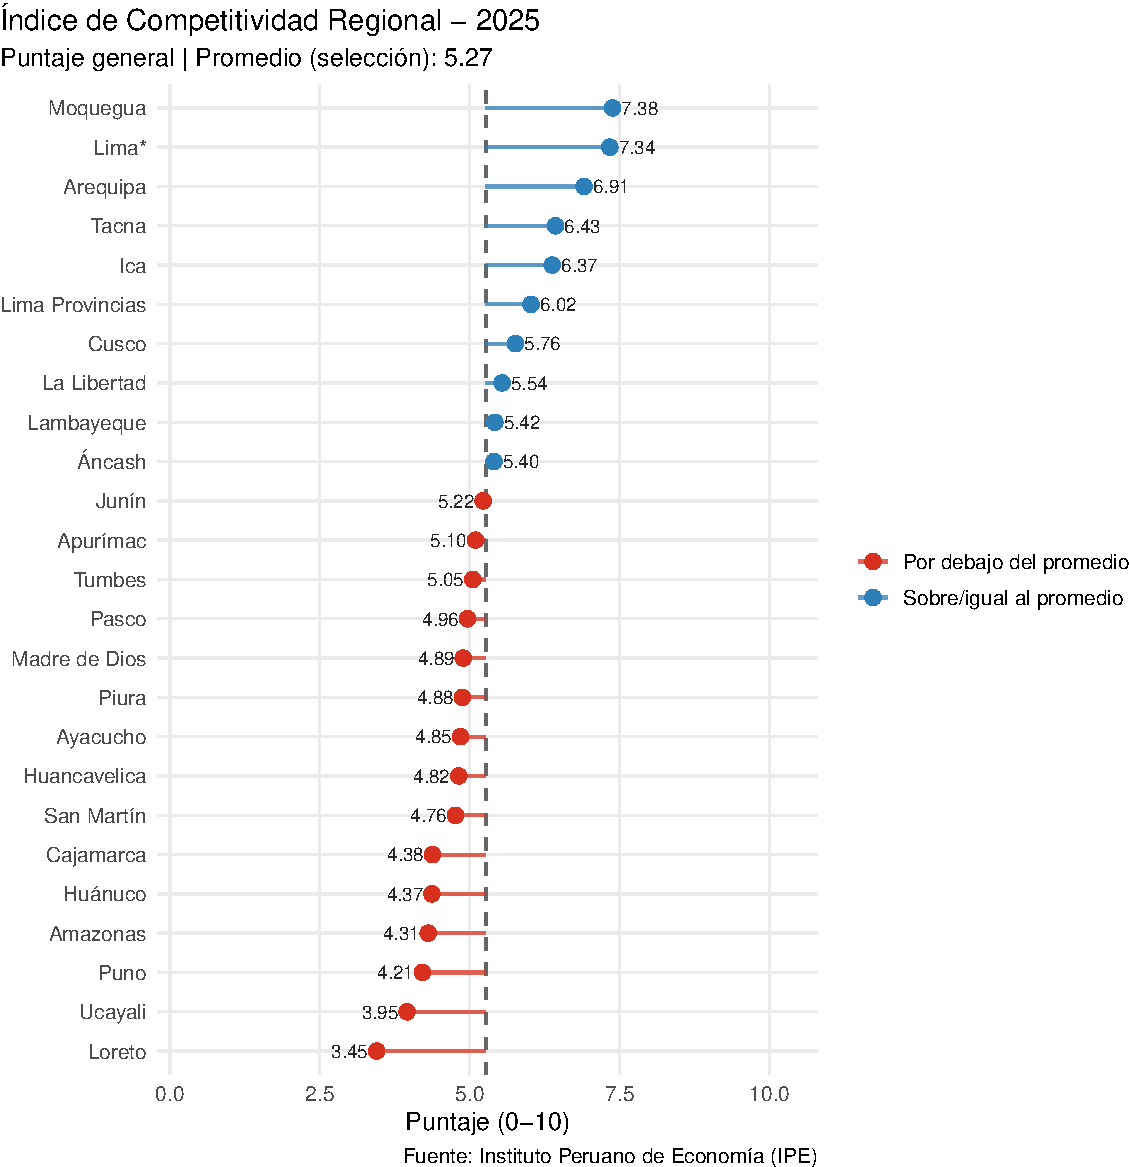
\includegraphics{Manual_files/figure-pdf/unnamed-chunk-47-1.pdf}

\textbf{Resultado esperado.} Dos clases: \textbf{por encima} (o igual)
vs.~\textbf{por debajo} del promedio de la selección. Útil para una
lectura ejecutiva rápida.

\paragraph{\texorpdfstring{\textbf{2) Pilar Salud con esquema divergente
(promedio
nacional)}}{2) Pilar Salud con esquema divergente (promedio nacional)}}\label{pilar-salud-con-esquema-divergente-promedio-nacional}

\textbf{Se desea lo siguiente:} visualizar la \textbf{distancia al
promedio nacional} en el pilar Salud, con gradiente continuo centrado en
0.

\begin{Shaded}
\begin{Highlighting}[]
\NormalTok{g2 }\OtherTok{\textless{}{-}} \FunctionTok{general\_media}\NormalTok{(}
  \AttributeTok{edicion =} \DecValTok{2025}\NormalTok{,}
  \AttributeTok{pilar   =} \StringTok{"SAL"}\NormalTok{,         }
  \AttributeTok{regiones =} \StringTok{"ALL"}\NormalTok{,}
  \AttributeTok{promedio\_nacional =} \ConstantTok{TRUE}\NormalTok{,}
  \AttributeTok{esquema =} \StringTok{"divergente"}\NormalTok{,}
  \AttributeTok{mostrar\_leyenda =} \ConstantTok{TRUE}
\NormalTok{)}
\NormalTok{g2}
\end{Highlighting}
\end{Shaded}

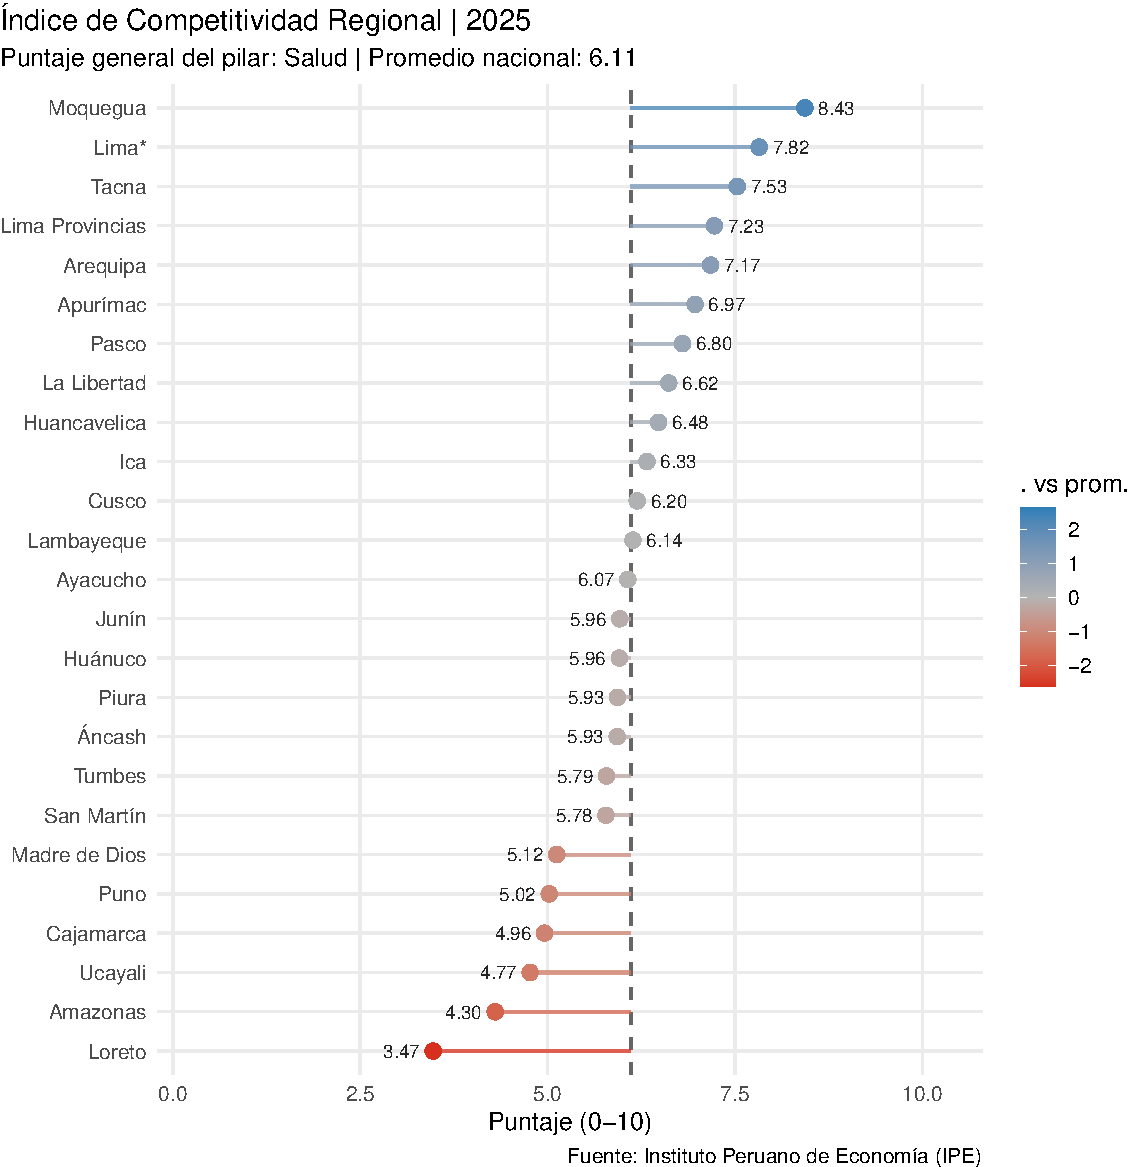
\includegraphics{Manual_files/figure-pdf/unnamed-chunk-48-1.pdf}

\textbf{Resultado esperado.} Colores fríos para \textbf{sobre} el
promedio nacional, cálidos para \textbf{bajo} el promedio, la leyenda
cuantifica la \textbf{diferencia}.

\paragraph{\texorpdfstring{\textbf{3) Subconjunto costero sin Lima *,
esquema
semaforo}}{3) Subconjunto costero sin Lima *, esquema semaforo}}\label{subconjunto-costero-sin-lima-esquema-semaforo}

\textbf{Se desea lo siguiente:} enfocar en la \textbf{costa}, excluir
\textbf{Lima}* y clasificar en \textbf{bajo/en torno/alto} respecto del
promedio \textbf{de la selección}.

\begin{Shaded}
\begin{Highlighting}[]
\NormalTok{g3 }\OtherTok{\textless{}{-}} \FunctionTok{general\_media}\NormalTok{(}
  \AttributeTok{edicion =} \DecValTok{2025}\NormalTok{,}
  \AttributeTok{pilar   =} \ConstantTok{NULL}\NormalTok{,                         }
  \AttributeTok{regiones =} \FunctionTok{c}\NormalTok{(}\StringTok{"gr\_costa"}\NormalTok{, }\StringTok{"{-}Lima*"}\NormalTok{),}
  \AttributeTok{promedio\_nacional =} \ConstantTok{FALSE}\NormalTok{,                }
  \AttributeTok{esquema =} \StringTok{"semaforo"}\NormalTok{,}
  \AttributeTok{mostrar\_leyenda =} \ConstantTok{TRUE}
\NormalTok{)}
\NormalTok{g3}
\end{Highlighting}
\end{Shaded}

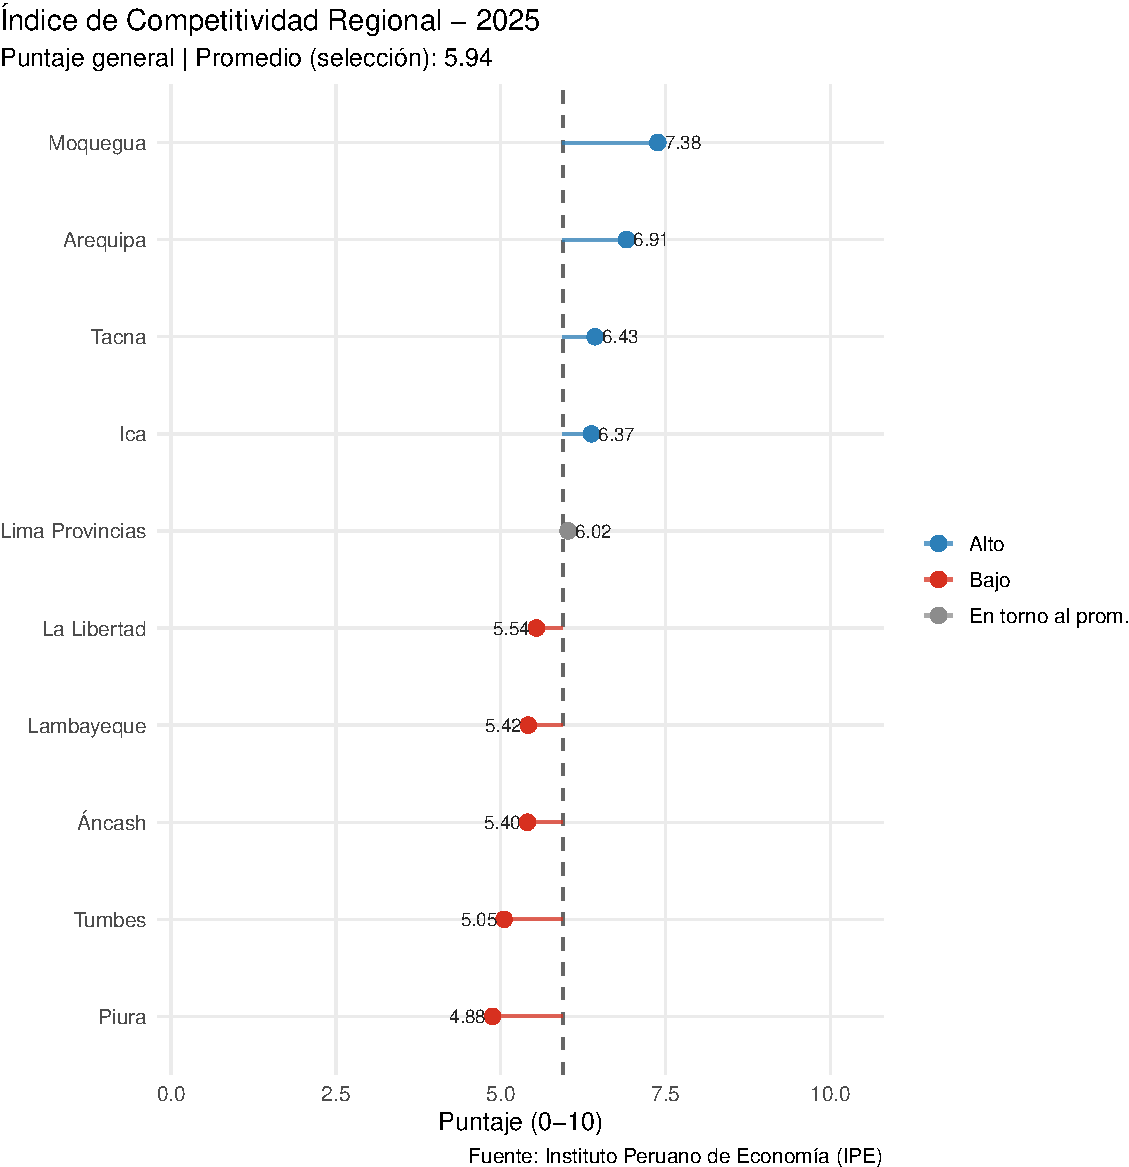
\includegraphics{Manual_files/figure-pdf/unnamed-chunk-49-1.pdf}

\textbf{Resultado esperado.} Tres bandas con tolerancia interna, útil
para audiencias que prefieren umbrales cualitativos claros.

\paragraph{\texorpdfstring{\textbf{4) Color por región (pilar
Infraestructura) y paleta
accesible}}{4) Color por región (pilar Infraestructura) y paleta accesible}}\label{color-por-regiuxf3n-pilar-infraestructura-y-paleta-accesible}

\textbf{Se desea lo siguiente:} resaltar la \textbf{identidad} de cada
región con una paleta cualitativa accesible.

\begin{Shaded}
\begin{Highlighting}[]
\NormalTok{g4 }\OtherTok{\textless{}{-}} \FunctionTok{general\_media}\NormalTok{(}
  \AttributeTok{edicion =} \DecValTok{2025}\NormalTok{,}
  \AttributeTok{pilar   =} \StringTok{"INF"}\NormalTok{,      }
  \AttributeTok{regiones =} \StringTok{"gr\_norte"}\NormalTok{,}
  \AttributeTok{promedio\_nacional =} \ConstantTok{TRUE}\NormalTok{,}
  \AttributeTok{esquema =} \StringTok{"region"}\NormalTok{,}
  \AttributeTok{paleta\_region =} \StringTok{"okabe\_ito"}\NormalTok{,}
  \AttributeTok{mostrar\_leyenda =} \ConstantTok{TRUE}
\NormalTok{)}
\NormalTok{g4}
\end{Highlighting}
\end{Shaded}

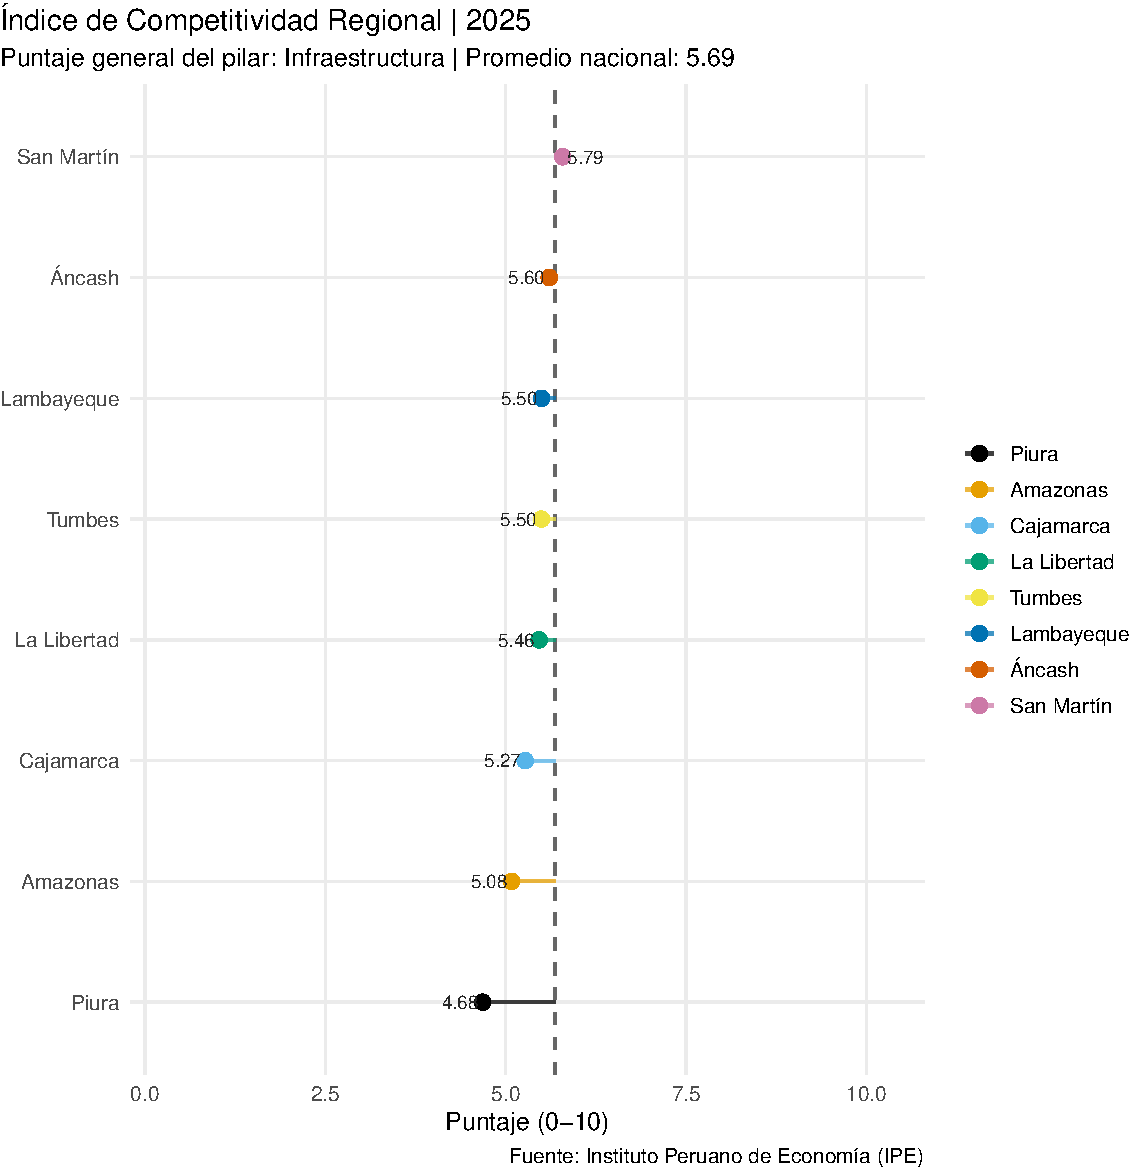
\includegraphics{Manual_files/figure-pdf/unnamed-chunk-50-1.pdf}

\textbf{Resultado esperado.} Una entrada por región con su color propio,
manteniendo la referencia del \textbf{promedio nacional} y la
comparabilidad 0--10.

\subsubsection{\texorpdfstring{\textbf{5) Diseño
monocromo}}{5) Diseño monocromo}}\label{diseuxf1o-monocromo}

\textbf{Se desea lo siguiente:} un gráfico para un bloque mixto de
regiones, enfatizando la distancia al promedio \textbf{nacional} sin
distracción cromática.

\begin{Shaded}
\begin{Highlighting}[]
\NormalTok{g5 }\OtherTok{\textless{}{-}} \FunctionTok{general\_media}\NormalTok{(}
  \AttributeTok{edicion =} \DecValTok{2025}\NormalTok{,}
  \AttributeTok{pilar   =} \FunctionTok{c}\NormalTok{(}\StringTok{"Educación"}\NormalTok{),   }\DocumentationTok{\#\# pilar por nombre}
  \AttributeTok{regiones =} \FunctionTok{c}\NormalTok{(}\StringTok{"gr\_sierra"}\NormalTok{, }\StringTok{"Arequipa"}\NormalTok{, }\StringTok{"La Libertad"}\NormalTok{),}
  \AttributeTok{promedio\_nacional =} \ConstantTok{TRUE}\NormalTok{,}
  \AttributeTok{esquema =} \StringTok{"monocromo"}\NormalTok{,}
  \AttributeTok{color\_mono =} \StringTok{"\#3B5B92"}\NormalTok{,}
  \AttributeTok{mostrar\_leyenda =} \ConstantTok{FALSE}
\NormalTok{)}
\NormalTok{g5}
\end{Highlighting}
\end{Shaded}

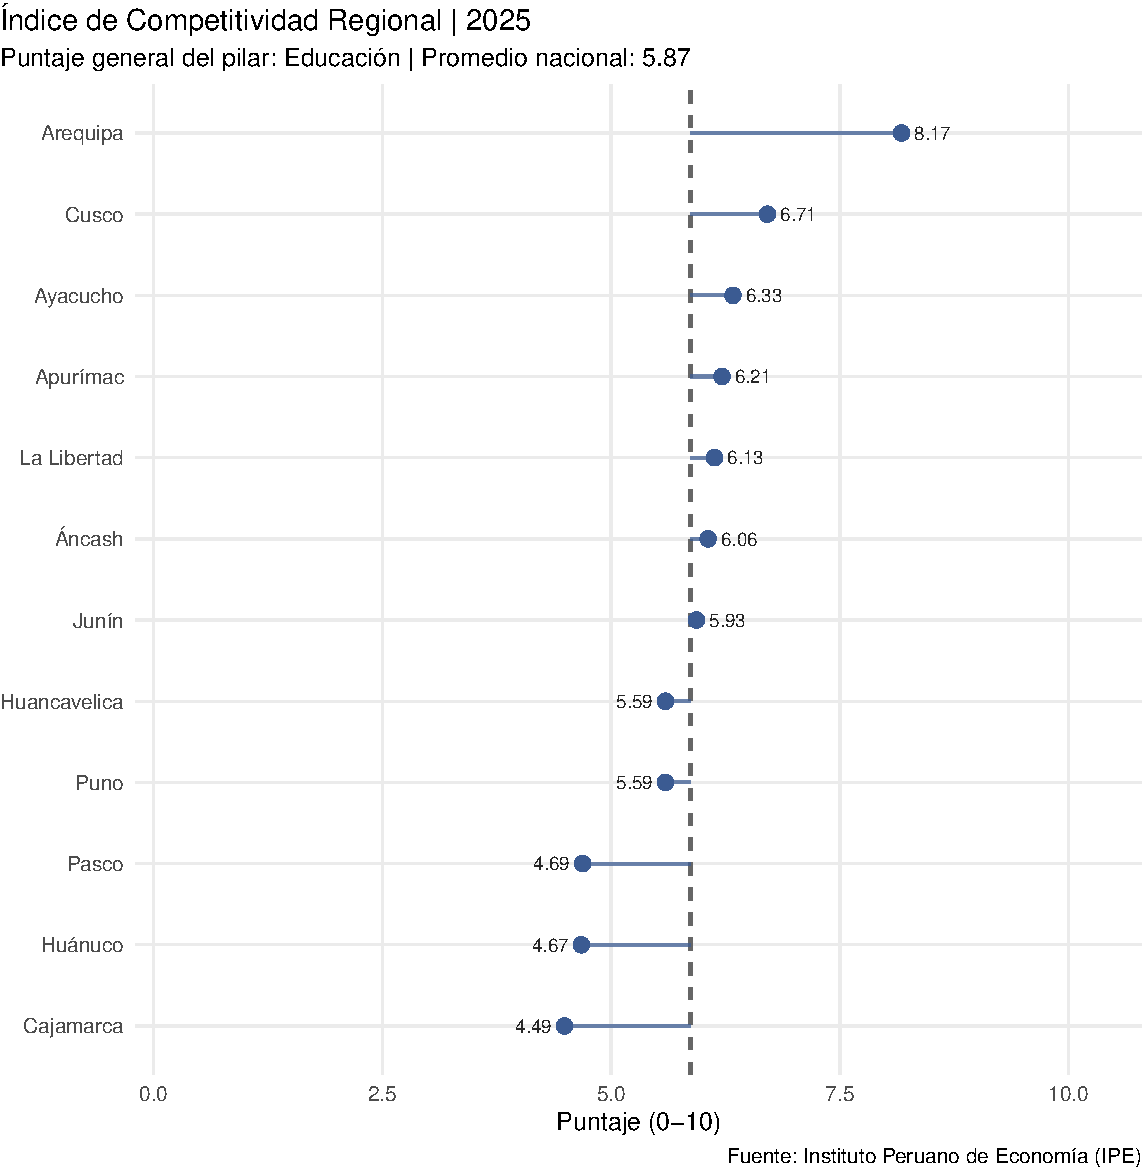
\includegraphics{Manual_files/figure-pdf/unnamed-chunk-51-1.pdf}

\textbf{Resultado esperado.} Segmentos y puntos en \textbf{un color}, la
interpretación se centra en la \textbf{dirección} y \textbf{magnitud} de
la diferencia frente al promedio nacional.

Perfecto. Aquí tienes el texto \textbf{detallado, narrativo y didáctico}
para tu manual sobre \textbf{general\_radar()}, con los
\textbf{parámetros clave en viñetas} (todas las opciones y valores
envueltos en ``) y \textbf{5 ejemplos} claros que exploran
funcionalidades propias del paquete (selección automática AUTO3, uso de
grupos `gr\_*`, control de paleta/alpha, puntos y formato de etiquetas
de ejes). Trato `usar\_codigos` como argumento secundario, mencionado en
la narración.

\subsection{\texorpdfstring{\textbf{general\_radar()}}{general\_radar()}}\label{general_radar}

\textbf{Telaraña del puntaje General por pilares (una edición)}

Orientada a representar, en \textbf{una edición} del INCORE, la
\textbf{configuración de puntajes por pilar} (escala 0--10) en un
\textbf{radar regular} (hexágono). Cada vértice corresponde a uno de los
\textbf{seis pilares}: Entorno económico, Laboral, Infraestructura,
Salud, Educación e Instituciones. La figura admite \textbf{comparar
varias regiones} superponiendo sus polígonos (lo ideal son \textbf{3--6}
para una lectura nítida).

\subsubsection{\texorpdfstring{\textbf{Introducción}}{Introducción}}\label{introducciuxf3n-9}

\texttt{general\_radar()} resuelve la necesidad de \textbf{comparar
perfiles} de competitividad por pilar entre regiones en un corte
temporal único. Mientras un ranking por pilar ordena y un mapa localiza,
la telaraña muestra la \textbf{forma} del desempeño: regiones con
\textbf{perfiles equilibrados} (polígonos cercanos a un círculo) frente
a otras con \textbf{fortalezas} y \textbf{debilidades} marcadas
(polígonos ``deformados'' hacia ciertos vértices).

La función puede \textbf{seleccionar automáticamente} tres casos
representativos (``AUTO3'', por defecto): \textbf{bajo}, \textbf{medio}
y \textbf{alto} según el \textbf{promedio simple de los seis pilares}.
Internamente, obtiene los puntajes con ind\_tabla(ediciones = edicion,
modo = ``pilares'', largo = TRUE) y los proyecta en coordenadas
cartesianas para dibujar \textbf{lados rectos}, facilitando la
comparación visual.

\subsubsection{\texorpdfstring{\textbf{Parámetros}}{Parámetros}}\label{paruxe1metros-8}

Trabajar con general\_radar() implica decidir: (i) \textbf{qué edición}
se dibuja, (ii) \textbf{qué regiones} se comparan (automáticas,
subconjuntos, grupos), y (iii) \textbf{cómo} presentar la figura
(paleta, transparencia de relleno, puntos y formato de etiquetas de
ejes). A continuación, los argumentos clave con sus opciones.

\begin{itemize}
\item
  \textbf{edicion}: define la \textbf{edición (año)} de la que se
  tomarán los puntajes por pilar.

  Opciones y formato:

  \begin{itemize}
  \item
    integer(1)
  \item
    Rango típico del INCORE: 2016 \ldots{} 2025
  \end{itemize}
\item
  \textbf{regiones}: controla \textbf{qué regiones} se superponen en el
  radar.

  Opciones y formato:

  \begin{itemize}
  \item
    ``AUTO3'' (por defecto): selección automática de \textbf{3} regiones
    representativas (\textbf{bajo/medio/alto}) según el
    \textbf{promedio} de los seis pilares.
  \item
    NULL: \textbf{todas} las regiones (no recomendado por legibilidad).
  \item
    Vector con nombres/códigos: c(``Arequipa'', ``Cusco'', ``La
    Libertad'') o c(``ARE'', ``CUS'', ``LAL'').
  \item
    Puede incluir \textbf{grupos gr\_*} cuando estén disponibles en tu
    ecosistema (p.~ej., ``gr\_costa''), combinados con regiones
    puntuales.
  \end{itemize}
\item
  \textbf{max\_regiones}: establece el \textbf{umbral de advertencia}
  por \textbf{legibilidad}.

  Opciones y formato:

  \begin{itemize}
  \item
    numeric(1), por defecto 6.
  \item
    Si el número de regiones supera este valor, se emite una
    \textbf{advertencia} (no detiene el gráfico).
  \end{itemize}
\item
  \textbf{alpha}: controla la \textbf{transparencia del relleno} de los
  polígonos (0--1).

  Opciones y formato:

  \begin{itemize}
  \item
    0.25 (por defecto)
  \item
    Valores mayores ⇒ \textbf{más opaco}, valores menores ⇒ \textbf{más
    transparente}.
  \end{itemize}
\item
  \textbf{paleta}: define la paleta \textbf{cualitativa} para colorear
  \textbf{por región}.

  Opciones y formato:

  \begin{itemize}
  \item
    ``ipe'' (por defecto, institucional)
  \item
    ``okabe\_ito'' (accesible para daltonismo)
  \item
    ``viridis'' (perceptualmente uniforme, aunque concebida para
    continuas, también útil aquí por contraste)
  \end{itemize}
\item
  \textbf{mostrar\_puntos}: decide si \textbf{marcar puntos} en los
  \textbf{vértices} de cada polígono (un punto por pilar).

  Opciones y formato:

  \begin{itemize}
  \item
    TRUE (por defecto)
  \item
    FALSE (limpia el gráfico cuando hay muchas regiones)
  \end{itemize}
\item
  \textbf{etiquetas\_pilares}: controla el \textbf{formato} de las
  \textbf{etiquetas} en los ejes del radar.

  Opciones y formato:

  \begin{itemize}
  \item
    ``corto'' (por defecto, quiebres de línea pensados para encajar
    mejor)
  \item
    ``largo'' (nombres completos en una sola línea)
  \end{itemize}
\end{itemize}

\subsubsection{\texorpdfstring{\textbf{Explicación
conceptual}}{Explicación conceptual}}\label{explicaciuxf3n-conceptual-8}

La función \textbf{lee} los puntajes por pilar de la \textbf{edición}
indicada (escala 0--10) y establece un \textbf{orden canónico} de
pilares para la disposición \textbf{hexagonal}. Si regiones = ``AUTO3'',
computa el \textbf{promedio de pilares} por región y selecciona
automáticamente \textbf{tres} casos representativos (mínimo, mediana,
máximo). Si se pasa un vector específico (o grupos gr\_*), filtra a esas
regiones.

Cada pilar se mapea a un \textbf{ángulo fijo} del hexágono y el puntaje
actúa como \textbf{radio}, pero la proyección es a \textbf{coordenadas
cartesianas} para dibujar \textbf{lados rectos}. Se añade una
\textbf{rejilla} de referencia (por ejemplo, 2--4--6--8--10) y los
\textbf{ejes} desde el centro a cada vértice con \textbf{etiquetas}
cortas o largas. La \textbf{paleta cualitativa} asigna color por región
y el \textbf{relleno} con alpha permite ver solapes al comparar.

En la lectura, \textbf{polígonos amplios} sugieren \textbf{desempeño
alto} generalizado, \textbf{deformaciones} hacia un vértice indican
\textbf{fortalezas} específicas, \textbf{huecos} o retracciones señalan
\textbf{áreas a mejorar}. Limitar el número de regiones maximiza la
\textbf{interpretabilidad}.

\subsubsection{\texorpdfstring{\textbf{Ejemplos}}{Ejemplos}}\label{ejemplos-8}

\paragraph{\texorpdfstring{\textbf{1) Selección automática de 3 regiones
(``AUTO3'') --- configuración
básica}}{1) Selección automática de 3 regiones (``AUTO3'') --- configuración básica}}\label{selecciuxf3n-automuxe1tica-de-3-regiones-auto3-configuraciuxf3n-buxe1sica}

\textbf{Se desea lo siguiente:} comparar \textbf{tres} perfiles
representativos (bajo/medio/alto) en la edición 2025 con formato legible
por defecto.

\begin{Shaded}
\begin{Highlighting}[]
\NormalTok{r1 }\OtherTok{\textless{}{-}} \FunctionTok{general\_radar}\NormalTok{(}
  \AttributeTok{edicion  =} \DecValTok{2025}\NormalTok{,}
  \AttributeTok{paleta   =} \StringTok{"ipe"}\NormalTok{,}
  \AttributeTok{alpha    =} \FloatTok{0.25}\NormalTok{,}
  \AttributeTok{mostrar\_puntos    =} \ConstantTok{TRUE}\NormalTok{,}
  \AttributeTok{etiquetas\_pilares =} \StringTok{"corto"}
\NormalTok{)}
\NormalTok{r1}
\end{Highlighting}
\end{Shaded}

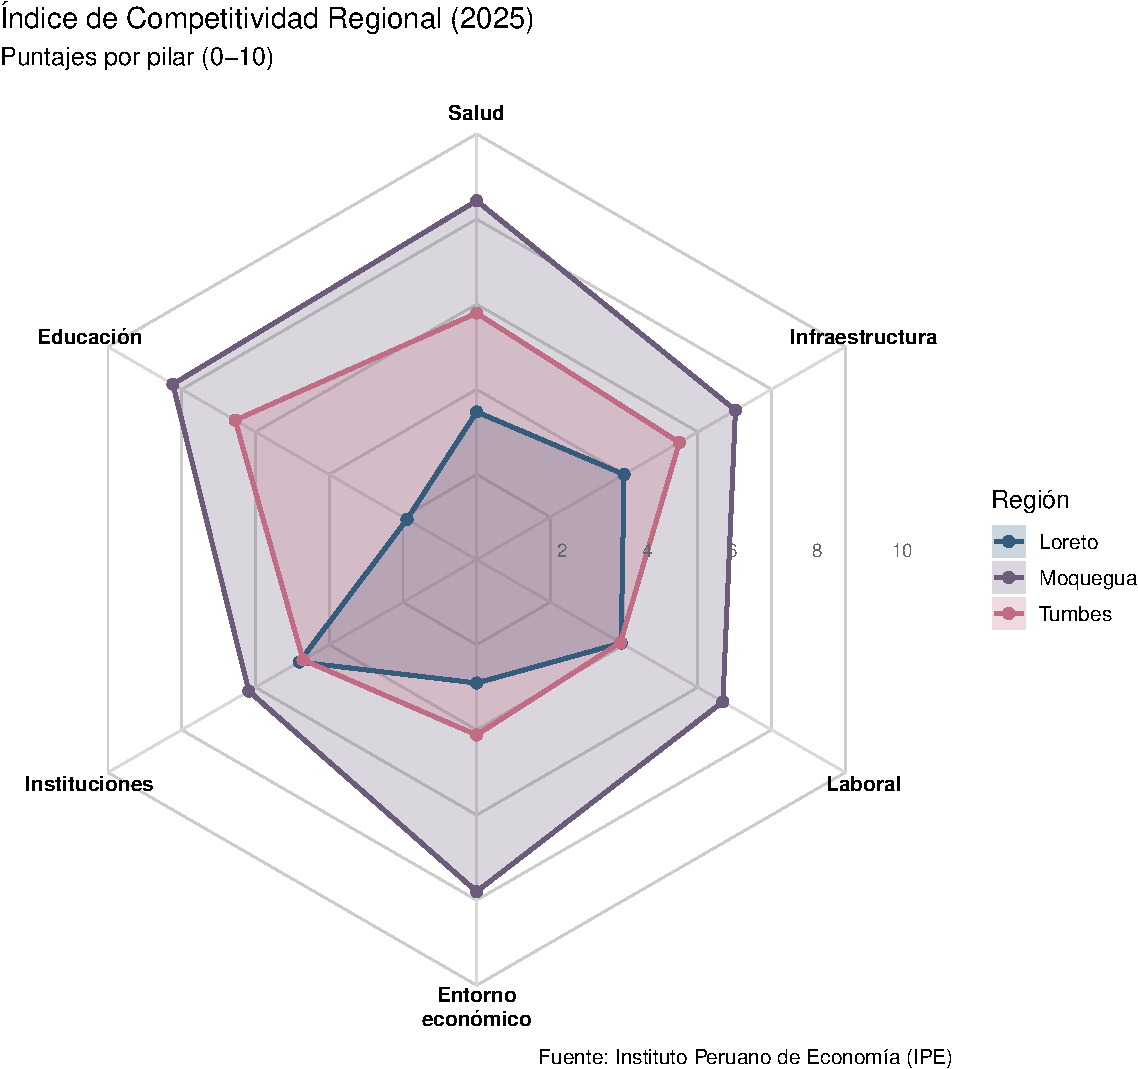
\includegraphics{Manual_files/figure-pdf/unnamed-chunk-52-1.pdf}

\textbf{Resultado esperado.} Un radar con \textbf{tres polígonos}: uno
``retraído'' (bajo), otro intermedio y otro ``expandido'' (alto),
facilitando la comparación pedagógica.

\paragraph{\texorpdfstring{\textbf{2) Subconjunto explícito de
regiones}}{2) Subconjunto explícito de regiones}}\label{subconjunto-expluxedcito-de-regiones}

\paragraph{\texorpdfstring{\textbf{Se desea lo siguiente:} comparar
\textbf{tres} regiones específicas usando una paleta accesible y nombres
completos en los
ejes.}{Se desea lo siguiente: comparar tres regiones específicas usando una paleta accesible y nombres completos en los ejes.}}\label{se-desea-lo-siguiente-comparar-tres-regiones-especuxedficas-usando-una-paleta-accesible-y-nombres-completos-en-los-ejes.}

\begin{Shaded}
\begin{Highlighting}[]
\NormalTok{r2 }\OtherTok{\textless{}{-}} \FunctionTok{general\_radar}\NormalTok{(}
  \AttributeTok{edicion  =} \DecValTok{2025}\NormalTok{,}
  \AttributeTok{regiones =} \FunctionTok{c}\NormalTok{(}\StringTok{"Arequipa"}\NormalTok{, }\StringTok{"Cusco"}\NormalTok{, }\StringTok{"La Libertad"}\NormalTok{),}
  \AttributeTok{paleta   =} \StringTok{"okabe\_ito"}\NormalTok{,}
  \AttributeTok{alpha    =} \FloatTok{0.30}\NormalTok{,}
  \AttributeTok{mostrar\_puntos    =} \ConstantTok{TRUE}\NormalTok{,}
  \AttributeTok{etiquetas\_pilares =} \StringTok{"largo"}
\NormalTok{)}
\NormalTok{r2}
\end{Highlighting}
\end{Shaded}

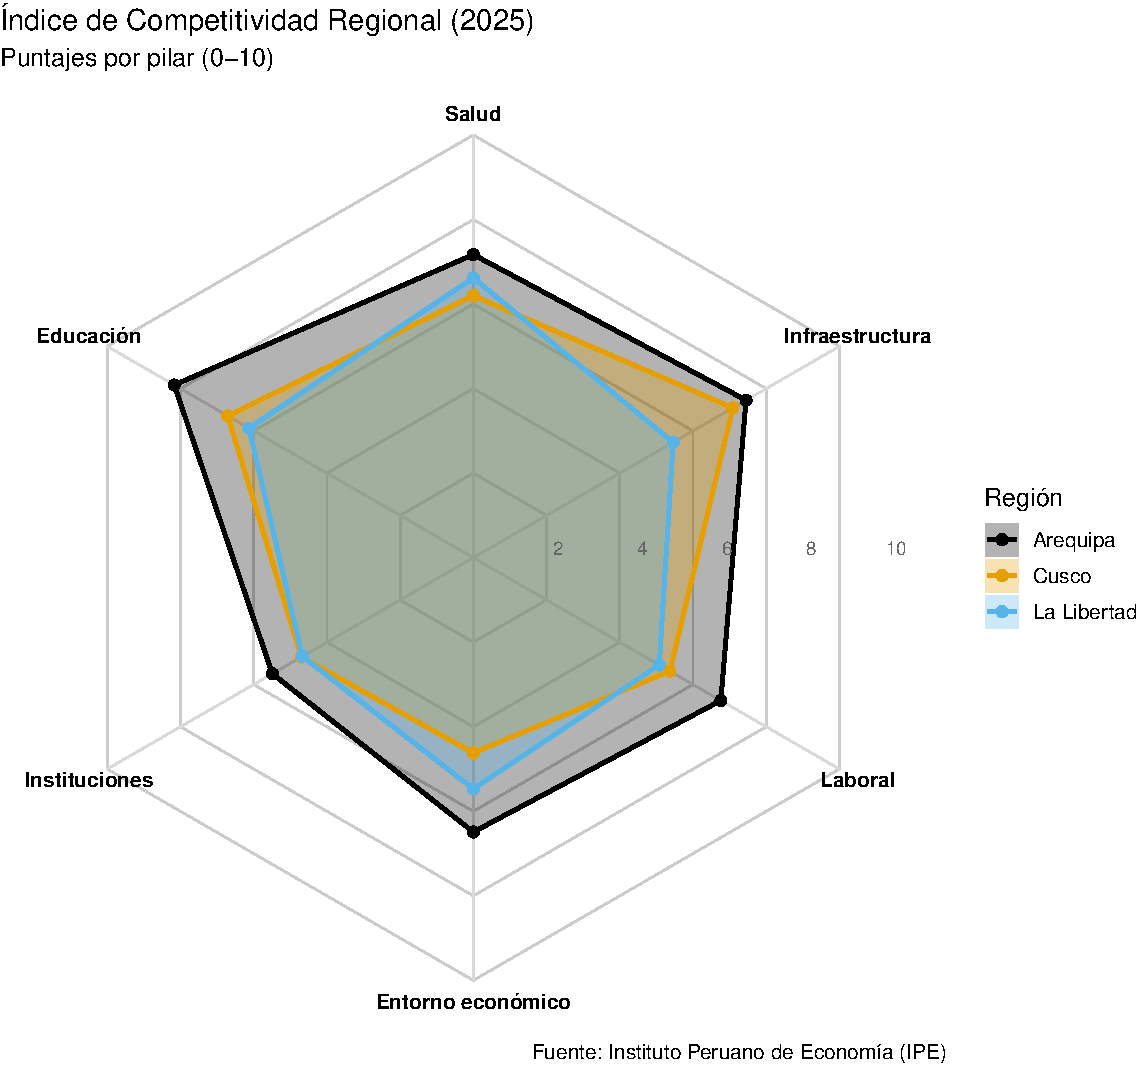
\includegraphics{Manual_files/figure-pdf/unnamed-chunk-53-1.pdf}

\textbf{Resultado esperado.} Tres polígonos con \textbf{alto contraste
cromático} y ejes con \textbf{etiquetas}

\paragraph{\texorpdfstring{\textbf{3) Uso de grupos gr (combinación con
región puntual) y mayor
transparencia}}{3) Uso de grupos gr (combinación con región puntual) y mayor transparencia}}\label{uso-de-grupos-gr-combinaciuxf3n-con-regiuxf3n-puntual-y-mayor-transparencia}

\textbf{Se desea lo siguiente:} contrastar un grupo regional con una
región puntual, reduciendo opacidad para ver mejor solapes.

\begin{Shaded}
\begin{Highlighting}[]
\NormalTok{r3 }\OtherTok{\textless{}{-}} \FunctionTok{general\_radar}\NormalTok{(}
  \AttributeTok{edicion  =} \DecValTok{2025}\NormalTok{,}
  \AttributeTok{regiones =} \FunctionTok{c}\NormalTok{(}\StringTok{"gr\_costa"}\NormalTok{, }\StringTok{"{-}Arequipa"}\NormalTok{, }\StringTok{"{-}Lima*"}\NormalTok{, }
               \StringTok{"{-}Lima Provincias"}\NormalTok{, }\StringTok{"{-}Ica"}\NormalTok{, }\StringTok{"{-}Moquegua"}\NormalTok{),}
  \AttributeTok{paleta   =} \StringTok{"viridis"}\NormalTok{,}
  \AttributeTok{alpha    =} \FloatTok{0.18}\NormalTok{,}
  \AttributeTok{mostrar\_puntos    =} \ConstantTok{TRUE}\NormalTok{,}
  \AttributeTok{etiquetas\_pilares =} \StringTok{"corto"}
\NormalTok{)}
\NormalTok{r3}
\end{Highlighting}
\end{Shaded}

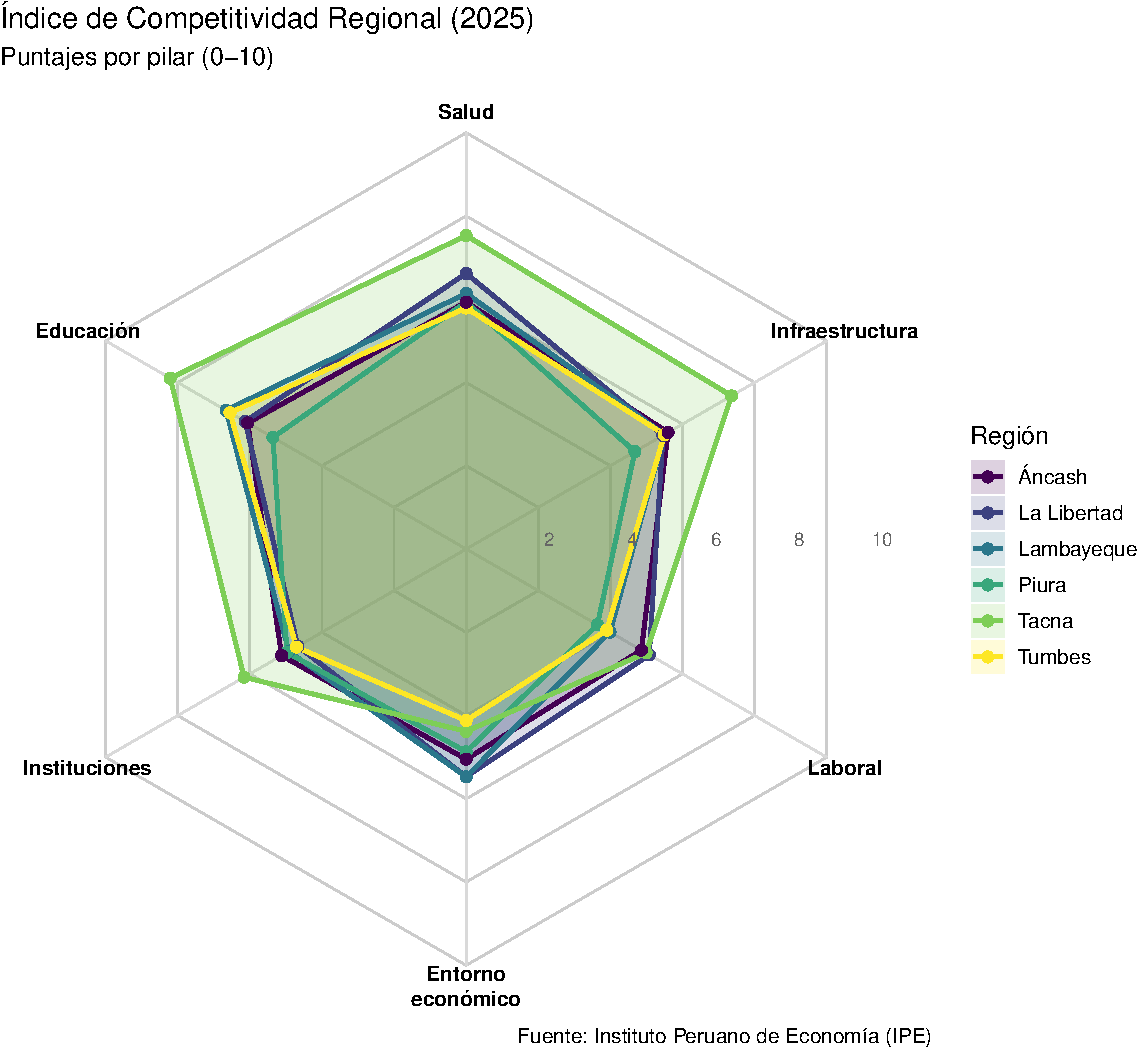
\includegraphics{Manual_files/figure-pdf/unnamed-chunk-54-1.pdf}

\textbf{Resultado esperado.} El polígono agregado del \textbf{grupo} (si
tu ecosistema expande gr\_costa a sus integrantes y filtra)

\paragraph{\texorpdfstring{\textbf{4) Comparación ampliada con
advertencia de
legibilidad}}{4) Comparación ampliada con advertencia de legibilidad}}\label{comparaciuxf3n-ampliada-con-advertencia-de-legibilidad}

\textbf{Se desea lo siguiente:} incluir \textbf{ocho} regiones (por
encima del umbral por defecto) para evaluar la \textbf{advertencia} y el
comportamiento visual.

\begin{Shaded}
\begin{Highlighting}[]
\NormalTok{r4 }\OtherTok{\textless{}{-}} \FunctionTok{general\_radar}\NormalTok{(}
  \AttributeTok{edicion  =} \DecValTok{2025}\NormalTok{,}
  \AttributeTok{regiones =} \FunctionTok{c}\NormalTok{(}\StringTok{"Arequipa"}\NormalTok{, }\StringTok{"Cusco"}\NormalTok{, }\StringTok{"La Libertad"}\NormalTok{,}
               \StringTok{"Piura"}\NormalTok{, }\StringTok{"Lambayeque"}\NormalTok{, }\StringTok{"Tacna"}\NormalTok{,}
               \StringTok{"Junín"}\NormalTok{, }\StringTok{"Puno"}\NormalTok{),}
  \AttributeTok{paleta   =} \StringTok{"ipe"}\NormalTok{,}
  \AttributeTok{alpha    =} \FloatTok{0.20}\NormalTok{,}
  \AttributeTok{mostrar\_puntos    =} \ConstantTok{FALSE}\NormalTok{,   }\DocumentationTok{\#\# sin puntos para reducir ruido}
  \AttributeTok{etiquetas\_pilares =} \StringTok{"corto"}     
\NormalTok{)}
\end{Highlighting}
\end{Shaded}

\begin{verbatim}
Warning in general_radar(edicion = 2025, regiones = c("Arequipa", "Cusco", :
Estás comparando 8 regiones. Para un radar legible, considera ≤ 6 (ideal 3–4).
\end{verbatim}

\begin{Shaded}
\begin{Highlighting}[]
\NormalTok{r4}
\end{Highlighting}
\end{Shaded}

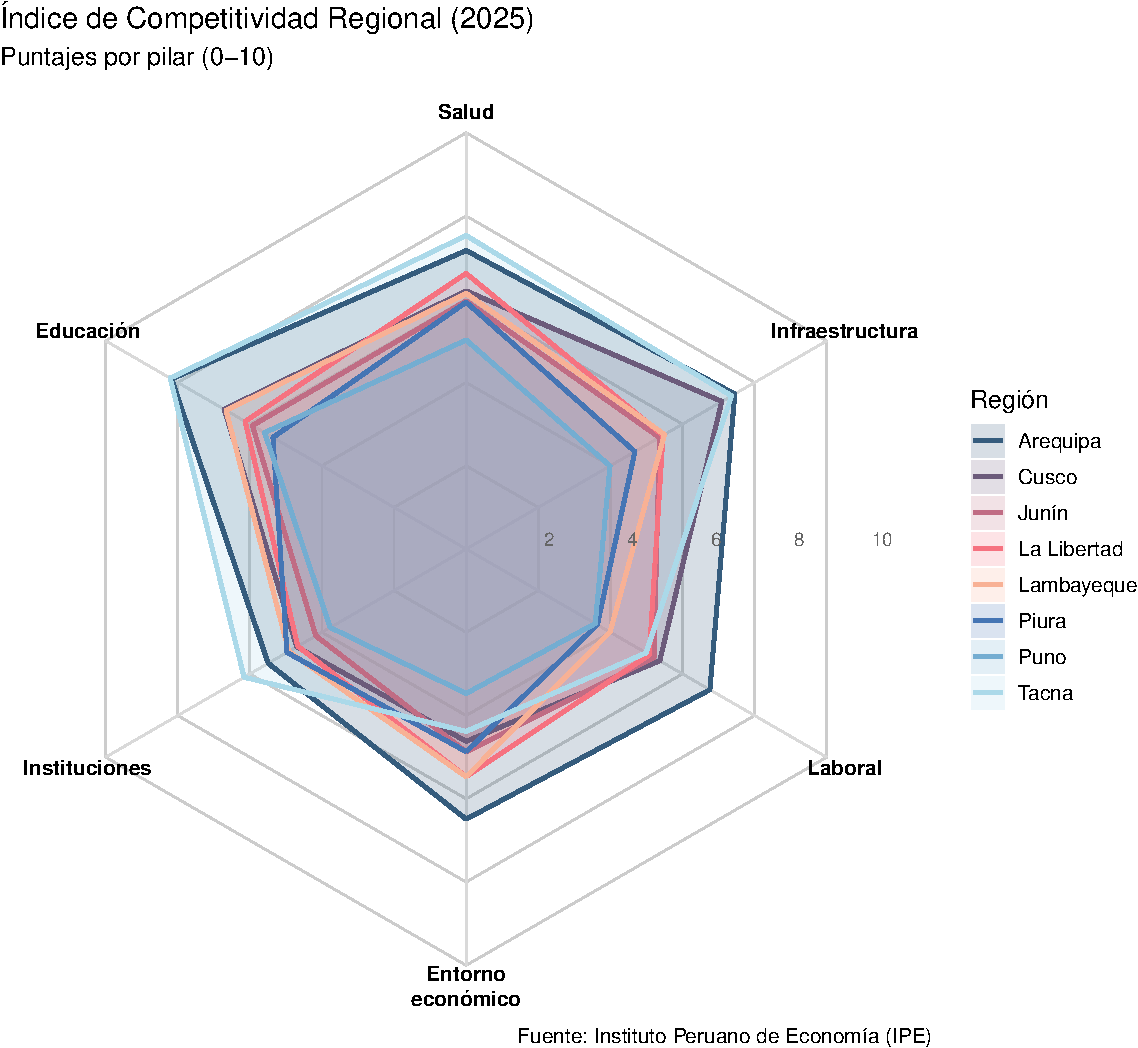
\includegraphics{Manual_files/figure-pdf/unnamed-chunk-55-1.pdf}

\textbf{Resultado esperado.} El gráfico \textbf{se renderiza} y muestra
los ocho polígonos, pero aparece una \textbf{advertencia} por
legibilidad. Se sugiere, para análisis fino, reducir el conjunto o
segmentar en dos gráficos.

\subsubsection{\texorpdfstring{\textbf{5) Comparación focalizada con
AUTO3 y estilo sin
puntos}}{5) Comparación focalizada con AUTO3 y estilo sin puntos}}\label{comparaciuxf3n-focalizada-con-auto3-y-estilo-sin-puntos}

\textbf{Se desea lo siguiente:} producir una figura \textbf{limpia} (sin
puntos) con la selección automática AUTO3, ajustando la transparencia
para enfatizar formas.

\begin{Shaded}
\begin{Highlighting}[]
\NormalTok{r5 }\OtherTok{\textless{}{-}} \FunctionTok{general\_radar}\NormalTok{(}
  \AttributeTok{edicion  =} \DecValTok{2025}\NormalTok{,}
  \AttributeTok{regiones =} \StringTok{"AUTO3"}\NormalTok{,}
  \AttributeTok{paleta   =} \StringTok{"ipe"}\NormalTok{,}
  \AttributeTok{alpha    =} \FloatTok{0.35}\NormalTok{,}
  \AttributeTok{mostrar\_puntos    =} \ConstantTok{FALSE}\NormalTok{,   }\DocumentationTok{\#\# limpia vértices para destacar contornos}
  \AttributeTok{etiquetas\_pilares =} \StringTok{"corto"}
\NormalTok{)}
\NormalTok{r5}
\end{Highlighting}
\end{Shaded}

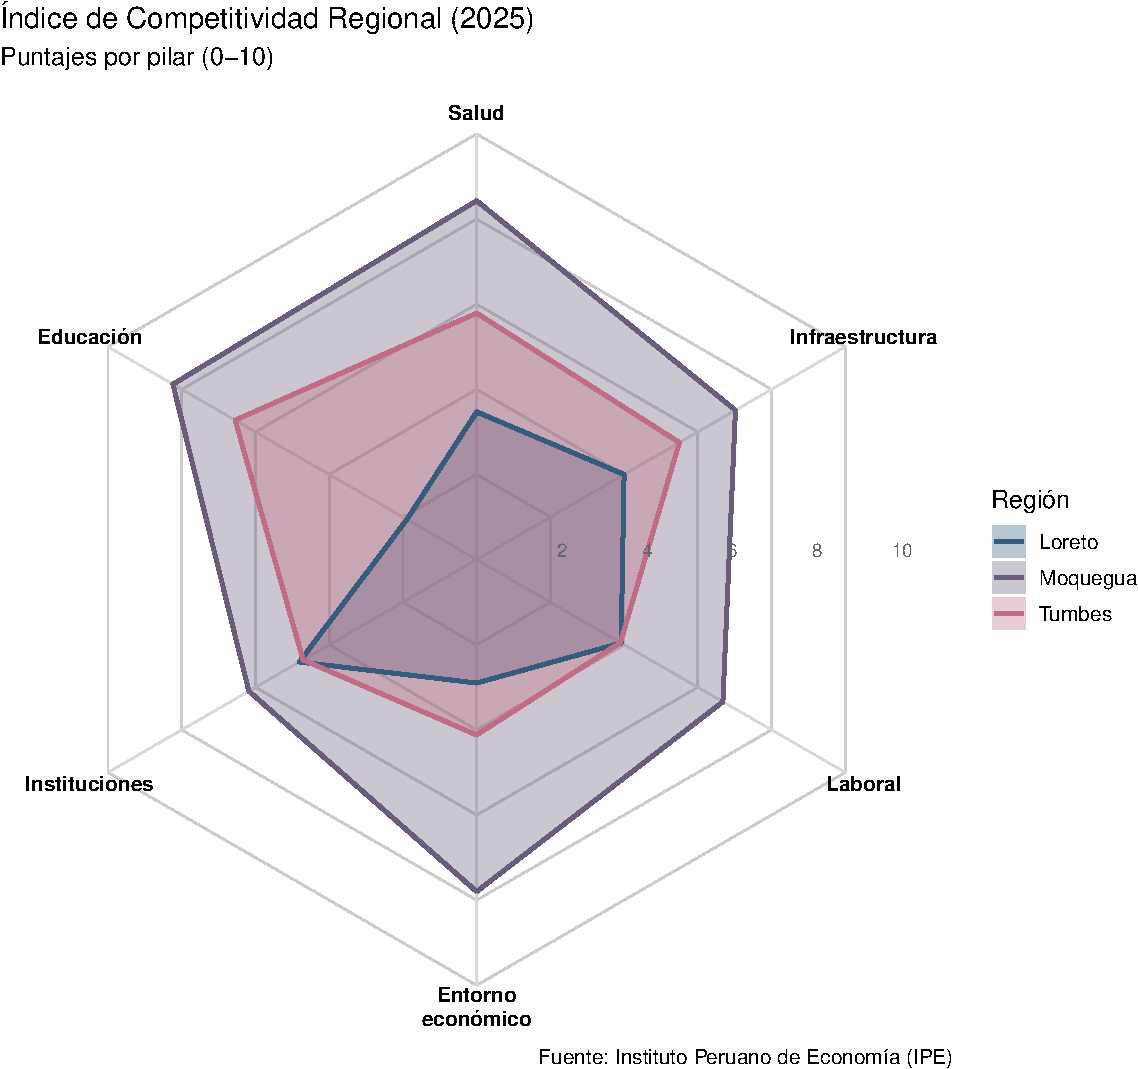
\includegraphics{Manual_files/figure-pdf/unnamed-chunk-56-1.pdf}

\textbf{Resultado esperado.} Tres polígonos con contornos nítidos y
relleno intermedio.

\section{\texorpdfstring{Familia \texttt{indc\_} y
\texttt{valor\_}}{Familia indc\_ y valor\_}}\label{familia-indc_-y-valor_}

\subsection{\texorpdfstring{\textbf{indc\_tabla(): indicadores por pilar
(puntajes
0--10)}}{indc\_tabla(): indicadores por pilar (puntajes 0--10)}}\label{indc_tabla-indicadores-por-pilar-puntajes-010}

\subsubsection{\texorpdfstring{\textbf{Descripción de
parámetros}}{Descripción de parámetros}}\label{descripciuxf3n-de-paruxe1metros}

\begin{itemize}
\item
  ediciones: vector numérico con una o más ediciones. Acepta formas como
  2025 o 2018:2025.
\item
  pilar: cadena con el pilar en \textbf{código} (``LAB'') o
  \textbf{nombre} (``Laboral'').
\item
  indicadores: ``ALL'' (todos los indicadores del pilar, salvo
  ``General''), o un vector de \textbf{códigos} (p.~ej., ``LAB2'') y/o
  \textbf{nombres} (p.~ej., ``2.2 Formalidad laboral'').
\item
  regiones: ``ALL'' o vector de \textbf{códigos/nombres} y
  \textbf{grupos} (p.~ej., ``gr\_costa''), con \textbf{exclusiones}
  mediante prefijo ``-'' (p.~ej., ``-Lima*'').
\item
  usar\_codigos: (mencionado) controla traducir códigos ↔ nombres en
  filtros.
\item
  incluir\_peru: (mencionado) si se desea mantener la fila
  \textbf{``Perú''}.
\item
  largo: TRUE devuelve \textbf{formato largo} (region, edicion,
  indicador, valor, usando \textbf{código} cuando esté disponible),
  FALSE devuelve \textbf{ancho}.
\item
  gt: TRUE produce una tabla \textbf{gt} con \emph{spanners} por
  edición, FALSE devuelve \textbf{tibble}.
\item
  verbose: TRUE imprime mensajes informativos.
\end{itemize}

\subsubsection{\texorpdfstring{\textbf{Explicación
conceptual}}{Explicación conceptual}}\label{explicaciuxf3n-conceptual-9}

La función filtra la base por \textbf{pilar} y \textbf{ediciones},
descarta la fila ``Perú'' (salvo que se pida), y elimina el indicador
\textbf{``General''} (a menos que se solicite todo). Luego
\textbf{promedia} internamente si aparecen duplicados esporádicos y
\textbf{redondea} a dos decimales. En salida \textbf{ancha}, las
columnas se nombran como CODIGO\_EDICION (por ejemplo, LAB2\_2025), si
un indicador no tiene código disponible, se genera un nombre limpio a
partir del título del indicador.

\subsubsection{\texorpdfstring{\textbf{Ejemplos}}{Ejemplos}}\label{ejemplos-9}

\begin{enumerate}
\def\labelenumi{\arabic{enumi}.}
\tightlist
\item
  \textbf{Tabla ancha} con todos los indicadores de un pilar en un rango
  de años
\end{enumerate}

\textbf{Se desea lo siguiente:} obtener, para el pilar LAB, una
\textbf{tabla por regiones} con dos indicadores en \textbf{columnas}
para las ediciones \textbf{2019--2025}.

\begin{Shaded}
\begin{Highlighting}[]
\NormalTok{tab1 }\OtherTok{\textless{}{-}} \FunctionTok{indc\_tabla}\NormalTok{(}
  \AttributeTok{ediciones    =} \DecValTok{2019}\SpecialCharTok{:}\DecValTok{2020}\NormalTok{,}
  \AttributeTok{pilar        =} \StringTok{"LAB"}\NormalTok{,}
  \AttributeTok{indicadores  =} \StringTok{"LAB3"}\NormalTok{,}
  \AttributeTok{regiones     =} \StringTok{"ALL"}\NormalTok{, }
  \AttributeTok{largo        =} \ConstantTok{FALSE}
\NormalTok{)}
\NormalTok{tab1}
\end{Highlighting}
\end{Shaded}

\begin{verbatim}
# A tibble: 25 x 3
   region       LAB3_2019 LAB3_2020
   <chr>            <dbl>     <dbl>
 1 Amazonas          2.27      2.66
 2 Apurímac          2.67      3.52
 3 Arequipa          6.94      7.49
 4 Ayacucho          3.25      3.23
 5 Cajamarca         0.16      1.64
 6 Cusco             4.92      5.31
 7 Huancavelica      2.14      0.77
 8 Huánuco           1.87      2.37
 9 Ica               7.38      8.48
10 Junín             4.05      4.66
# i 15 more rows
\end{verbatim}

\begin{quote}
Se espera un tibble con columnas tipo LAB1\_2019, LAB1\_2020 por región.
\end{quote}

\begin{enumerate}
\def\labelenumi{\arabic{enumi}.}
\setcounter{enumi}{1}
\tightlist
\item
  \textbf{Formato largo} para graficar con ggplot2
\end{enumerate}

\textbf{Se desea lo siguiente:} obtener datos \textbf{largos} del pilar
ECO en \textbf{2025}, listos para facetear por indicador.

\begin{Shaded}
\begin{Highlighting}[]
\NormalTok{tab\_long }\OtherTok{\textless{}{-}} \FunctionTok{indc\_tabla}\NormalTok{(}
  \AttributeTok{ediciones    =} \DecValTok{2025}\NormalTok{,}
  \AttributeTok{pilar        =} \StringTok{"ECO"}\NormalTok{,}
  \AttributeTok{indicadores  =} \StringTok{"ALL"}\NormalTok{,}
  \AttributeTok{regiones     =} \StringTok{"ALL"}\NormalTok{,}
  \AttributeTok{largo        =} \ConstantTok{TRUE}\NormalTok{,}
\NormalTok{)}
\NormalTok{tab\_long }\SpecialCharTok{|\textgreater{}} 
  \FunctionTok{head}\NormalTok{(}\DecValTok{10}\NormalTok{)}
\end{Highlighting}
\end{Shaded}

\begin{verbatim}
# A tibble: 10 x 4
   region   edicion indicador valor
   <chr>      <int> <chr>     <dbl>
 1 Amazonas    2025 ECO1       1.28
 2 Amazonas    2025 ECO2       2.52
 3 Amazonas    2025 ECO3       3.78
 4 Amazonas    2025 ECO4       0.45
 5 Amazonas    2025 ECO5       9.11
 6 Amazonas    2025 ECO6       2.88
 7 Amazonas    2025 ECO7       3.84
 8 Apurímac    2025 ECO1       3   
 9 Apurímac    2025 ECO2       2.52
10 Apurímac    2025 ECO3       2.8 
\end{verbatim}

\begin{quote}
Se espera region, edicion, indicador y valor (0--10).
\end{quote}

\begin{enumerate}
\def\labelenumi{\arabic{enumi}.}
\setcounter{enumi}{2}
\tightlist
\item
  \textbf{Selección de indicadores por código y nombre}
\end{enumerate}

\textbf{Se desea lo siguiente:} limitar a \textbf{tres} indicadores del
pilar LAB en \textbf{2024--2025} (mezclando código y nombre).

\begin{Shaded}
\begin{Highlighting}[]
\NormalTok{sel }\OtherTok{\textless{}{-}} \FunctionTok{c}\NormalTok{(}\StringTok{"LAB1"}\NormalTok{, }\StringTok{"2.2 Formalidad laboral"}\NormalTok{, }\StringTok{"LAB5"}\NormalTok{)}

\NormalTok{tab\_sel }\OtherTok{\textless{}{-}} \FunctionTok{indc\_tabla}\NormalTok{(}
  \AttributeTok{ediciones    =} \DecValTok{2025}\NormalTok{,}
  \AttributeTok{pilar        =} \StringTok{"LAB"}\NormalTok{,}
  \AttributeTok{indicadores  =}\NormalTok{ sel,}
  \AttributeTok{regiones     =} \StringTok{"ALL"}\NormalTok{,}
  \AttributeTok{usar\_codigos =} \ConstantTok{TRUE}
\NormalTok{)}
\NormalTok{tab\_sel}
\end{Highlighting}
\end{Shaded}

\begin{verbatim}
# A tibble: 25 x 4
   region       LAB1_2025 LAB2_2025 LAB5_2025
   <chr>            <dbl>     <dbl>     <dbl>
 1 Amazonas          2.15      3.99      3.12
 2 Apurímac          3.44      3.53      2.81
 3 Arequipa          8.68      7.43     10   
 4 Ayacucho          2.78      0.9       1.47
 5 Cajamarca         3.49      3.4       2.64
 6 Cusco             3.1       4.62      3.99
 7 Huancavelica      1.51      3.38      3.16
 8 Huánuco           2.79      3.8       1.93
 9 Ica               5.7       4.95      7.78
10 Junín             4.21      4.02      5.39
# i 15 more rows
\end{verbatim}

\begin{quote}
Se espera una \textbf{tabla ancha} únicamente con las columnas de esos
\textbf{indicadores×edición}.
\end{quote}

\begin{enumerate}
\def\labelenumi{\arabic{enumi}.}
\setcounter{enumi}{3}
\tightlist
\item
  \textbf{Con grupos y exclusiones de regiones}
\end{enumerate}

\textbf{Se desea lo siguiente:} incluir \textbf{Costa} y
\textbf{Sierra}, \textbf{excluyendo} Lima Metropolitana, para LAB en
\textbf{2025}.

\begin{Shaded}
\begin{Highlighting}[]
\NormalTok{tab\_reg }\OtherTok{\textless{}{-}} \FunctionTok{indc\_tabla}\NormalTok{(}
  \AttributeTok{ediciones    =} \DecValTok{2025}\NormalTok{,}
  \AttributeTok{pilar        =} \StringTok{"LAB"}\NormalTok{,}
  \AttributeTok{indicadores  =} \FunctionTok{c}\NormalTok{(}\StringTok{"LAB4"}\NormalTok{, }\StringTok{"LAB5"}\NormalTok{, }\StringTok{"LAB6"}\NormalTok{),}
  \AttributeTok{regiones     =} \FunctionTok{c}\NormalTok{(}\StringTok{"gr\_costa"}\NormalTok{, }\StringTok{"gr\_sierra"}\NormalTok{, }\StringTok{"{-}Lima*"}\NormalTok{)}
\NormalTok{)}
\NormalTok{tab\_reg}
\end{Highlighting}
\end{Shaded}

\begin{verbatim}
# A tibble: 19 x 4
   region          LAB4_2025 LAB5_2025 LAB6_2025
   <chr>               <dbl>     <dbl>     <dbl>
 1 Apurímac             7.03      2.81      7.37
 2 Arequipa             5.85     10         5.89
 3 Ayacucho             6         1.47      7.53
 4 Cajamarca            5.84      2.64      4.82
 5 Cusco                7.24      3.99      8.61
 6 Huancavelica         7.97      3.16      9.31
 7 Huánuco              5         1.93      4.39
 8 Ica                  6.28      7.78      5.93
 9 Junín                7.86      5.39      6.93
10 La Libertad          6.21      5.51      3.5 
11 Lambayeque           4.83      5.42      3.95
12 Lima Provincias      6.08      5.55      4.64
13 Moquegua             5.56      8.99      6.56
14 Pasco                6.15      5.62      4.12
15 Piura                5.83      3.81      3.25
16 Puno                 5.01      3.98      8.69
17 Tacna                3.22      6.46      5.75
18 Tumbes               2.97      4.74      2.56
19 Áncash               5.99      4.55      5.34
\end{verbatim}

\begin{quote}
Se espera una tabla por \textbf{regiones filtradas}, Lima* queda
excluida.
\end{quote}

\begin{enumerate}
\def\labelenumi{\arabic{enumi}.}
\setcounter{enumi}{4}
\tightlist
\item
  \textbf{Salida gt con spanners por edición}
\end{enumerate}

\textbf{Se desea lo siguiente:} una \textbf{tabla presentable} para el
pilar LAB en \textbf{2024--2025}, con encabezados por edición.

\begin{Shaded}
\begin{Highlighting}[]
\NormalTok{tab\_gt }\OtherTok{\textless{}{-}} \FunctionTok{indc\_tabla}\NormalTok{(}
  \AttributeTok{ediciones    =} \DecValTok{2024}\SpecialCharTok{:}\DecValTok{2025}\NormalTok{,}
  \AttributeTok{pilar        =} \StringTok{"LAB"}\NormalTok{,}
  \AttributeTok{indicadores  =} \StringTok{"ALL"}\NormalTok{,}
  \AttributeTok{regiones     =} \StringTok{"ALL"}\NormalTok{,}
  \AttributeTok{gt           =} \ConstantTok{TRUE}
\NormalTok{)}
\end{Highlighting}
\end{Shaded}

\begin{center}
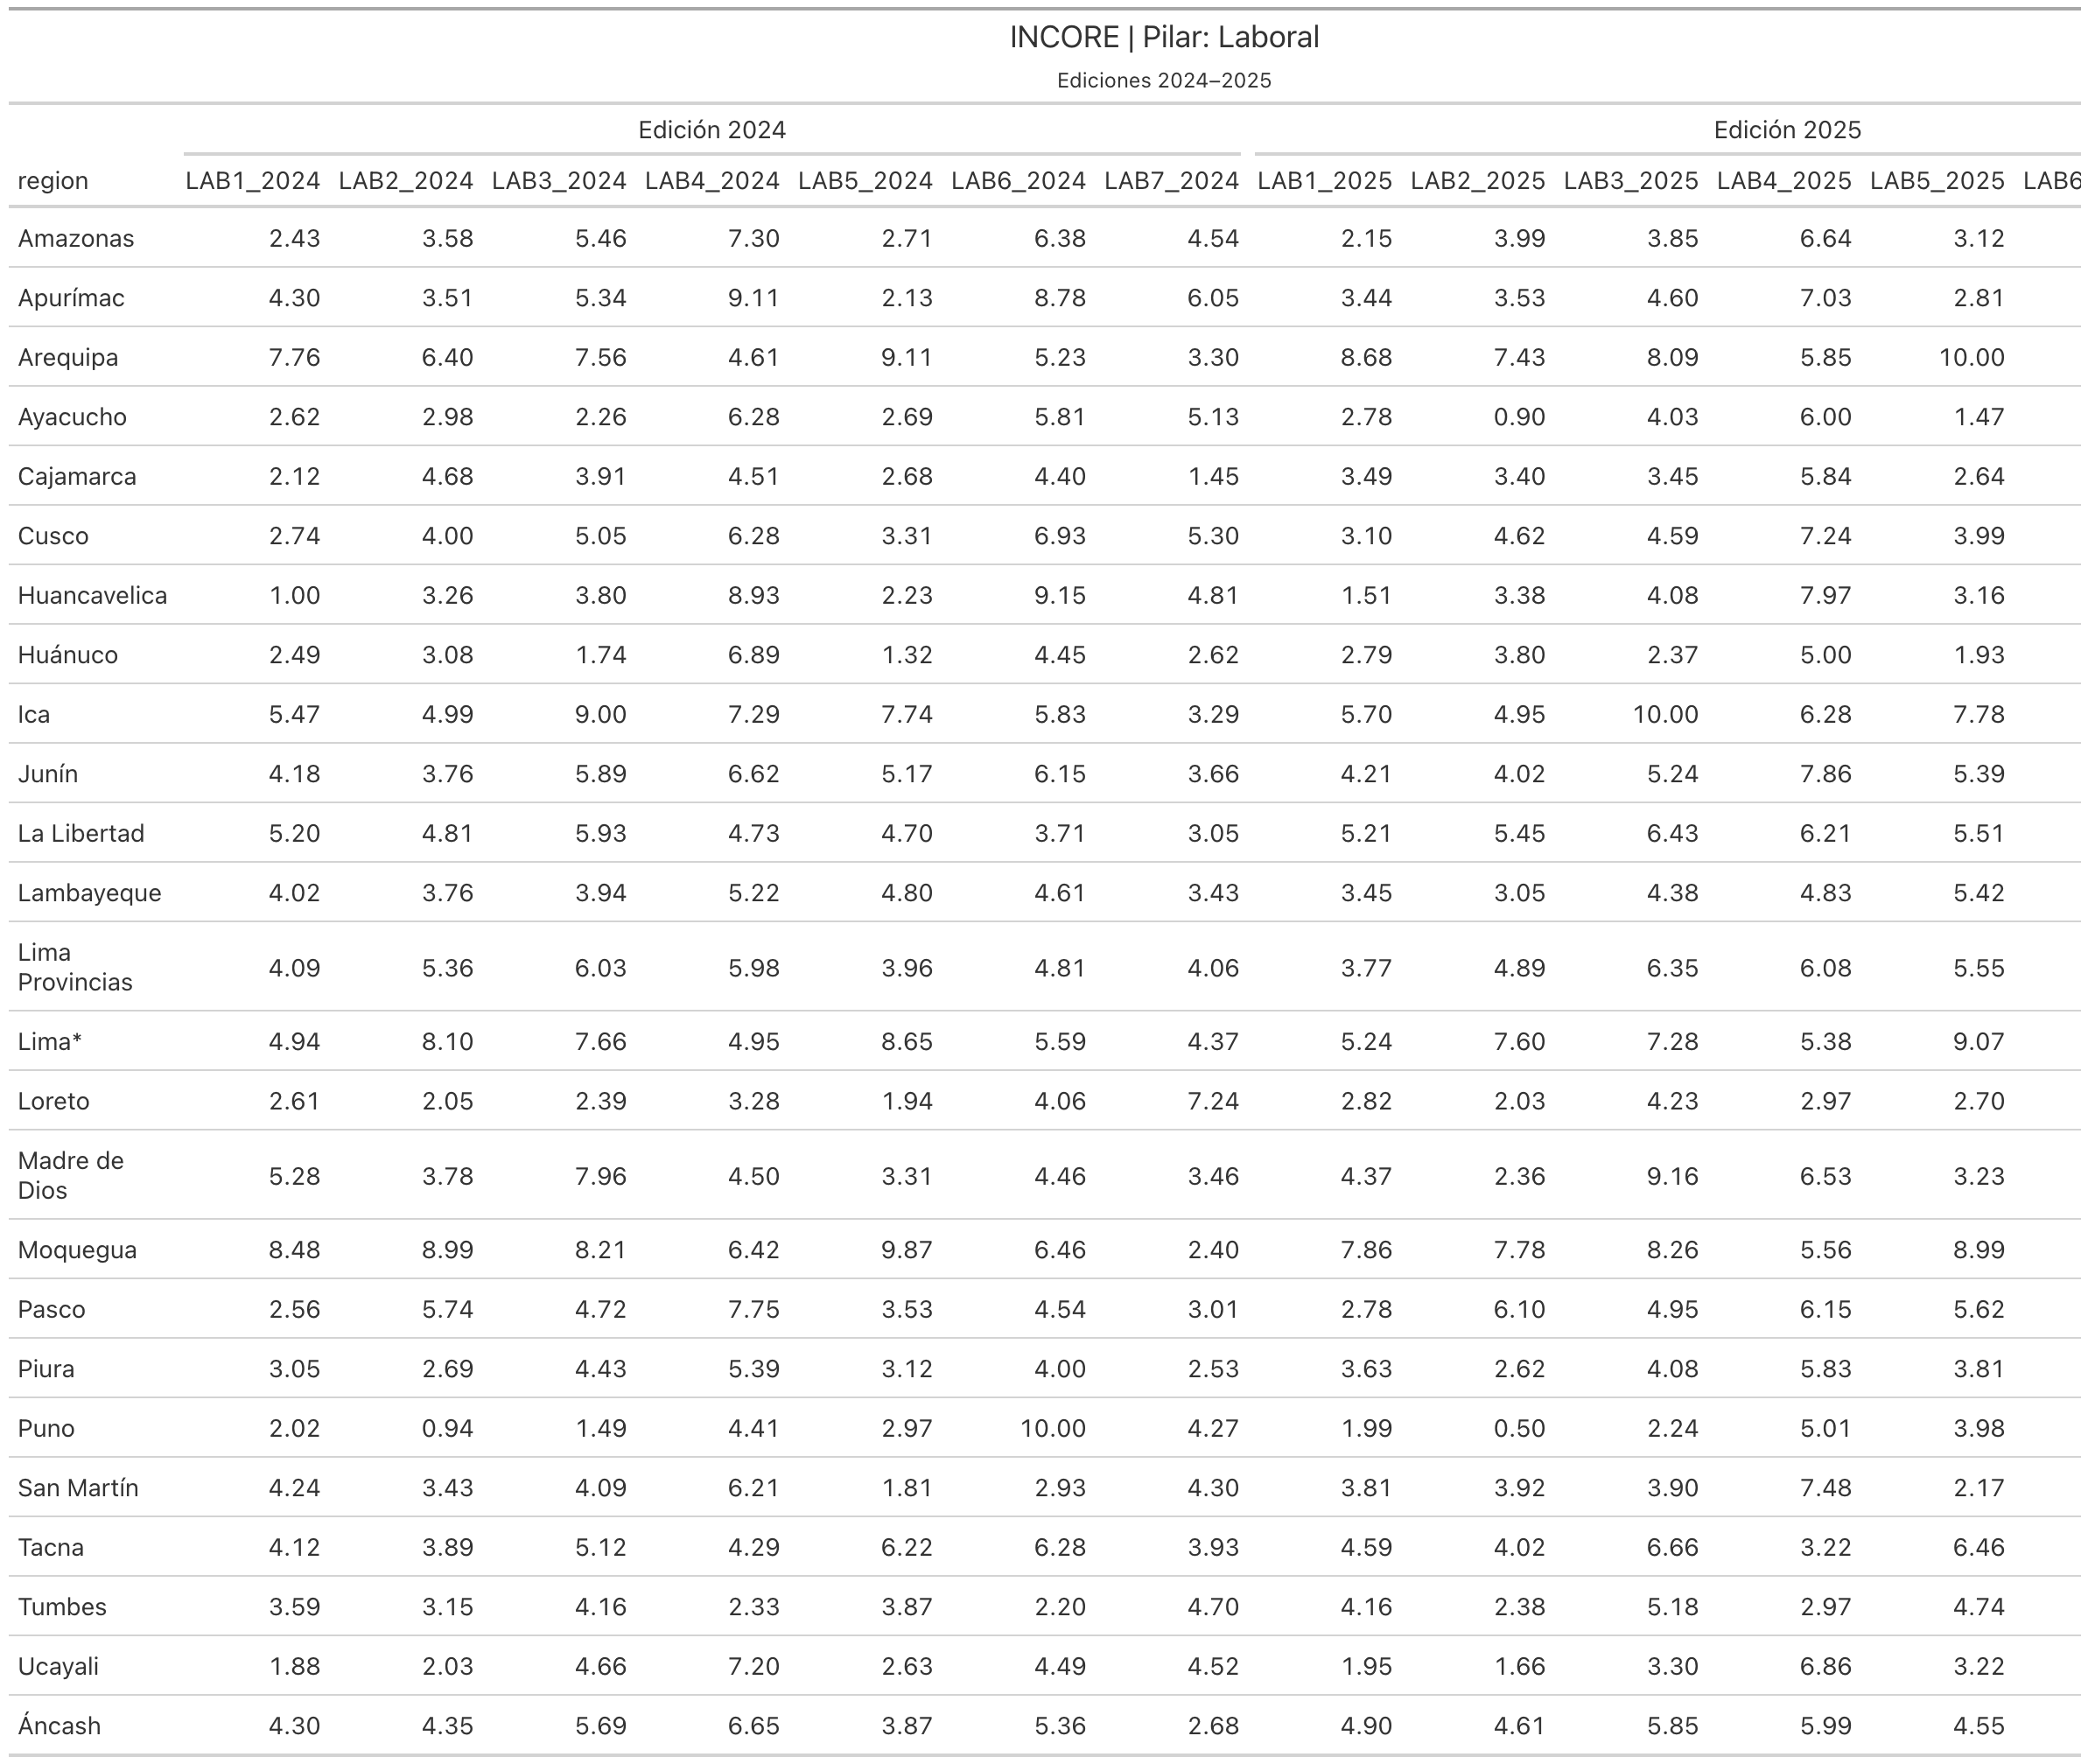
\includegraphics[width=0.9\textwidth,height=\textheight]{trem.png}
\end{center}

\begin{quote}
Se espera una \textbf{tabla gt} con \emph{spanners} por edición y
números a 2 decimales.
\end{quote}

¿Así, tal cual, te sirve para pegarlo directo a tu Quarto? Si quieres,
armo la subsección de \textbf{valores} (valor\_tabla) con el mismo
patrón.

\subsection{\texorpdfstring{\textbf{valor\_tabla(): valores originales
por indicador (con
unidad/fuente)}}{valor\_tabla(): valores originales por indicador (con unidad/fuente)}}\label{valor_tabla-valores-originales-por-indicador-con-unidadfuente}

\subsubsection{\texorpdfstring{\textbf{Descripción de
parámetros}}{Descripción de parámetros}}\label{descripciuxf3n-de-paruxe1metros-1}

\begin{itemize}
\item
  ediciones: vector numérico con una o más ediciones. Acepta formas como
  2025 o 2018:2025.
\item
  pilar: cadena con el pilar en \textbf{código} (``ECO'') o
  \textbf{nombre} (``Entorno económico'').
\item
  indicadores: ``ALL'' (todos los del pilar) o vector de
  \textbf{códigos/nombres}, admite entradas que \textbf{empiezan en
  número} (p.~ej., ``3'' o ``3.1 \ldots{}'') mapeadas a ECO3 dentro del
  pilar.
\item
  regiones: ``ALL'' o vector de \textbf{códigos/nombres}, también puede
  usar \textbf{grupos} y \textbf{exclusiones} (si los helpers de tu
  paquete lo permiten en valores).
\item
  usar\_codigos: (mencionado) controla traducciones en filtros.
\item
  incluir\_peru: (mencionado) si se desea mantener \textbf{``Perú''}.
\item
  largo: TRUE devuelve \textbf{formato largo} con region, edicion,
  indicador, valor, unidad, fuente, FALSE devuelve \textbf{ancho}.
\item
  gt: TRUE produce \textbf{gt} con \emph{spanners} por edición, FALSE
  devuelve \textbf{tibble}.
\item
  verbose: TRUE imprime mensajes informativos.
\end{itemize}

\subsubsection{\texorpdfstring{\textbf{Explicación
conceptual}}{Explicación conceptual}}\label{explicaciuxf3n-conceptual-10}

A diferencia de indc\_tabla(), esta función trabaja con \textbf{valores
originales} (no normalizados a 0--10). Por diseño \textbf{excluye}
unidad == ``Puntaje del 0 al 10''. Resuelve los \textbf{indicadores}
contra un catálogo (code ↔ name), acepta atajos como ``3'' dentro del
pilar (→ ECO3/LAB3 según corresponda), y \textbf{promedia} si existen
duplicados esporádicos. En salida ancha, las columnas se nombran como
CODIGO\_EDICION (o un nombre limpio cuando el código no esté
disponible). La salida larga conserva \textbf{unidad} y \textbf{fuente},
lo que resulta útil para rótulos y \emph{captions} de gráficos.

\subsubsection{\texorpdfstring{\textbf{Ejemplos}}{Ejemplos}}\label{ejemplos-10}

\begin{enumerate}
\def\labelenumi{\arabic{enumi}.}
\tightlist
\item
  \textbf{Valores anchos para un pilar en múltiples ediciones}
\end{enumerate}

\textbf{Se desea lo siguiente:} obtener los \textbf{valores (no
puntaje)} del pilar \textbf{ECO} entre \textbf{2020--2025} para
\textbf{todas} las regiones, en formato ancho.

\begin{Shaded}
\begin{Highlighting}[]
\NormalTok{val1 }\OtherTok{\textless{}{-}} \FunctionTok{valor\_tabla}\NormalTok{(}\AttributeTok{ediciones =} \DecValTok{2020}\SpecialCharTok{:}\DecValTok{2025}\NormalTok{, }
                    \AttributeTok{pilar =} \StringTok{"ECO"}\NormalTok{,}
                    \AttributeTok{indicadores =} \StringTok{"ECO1"}\NormalTok{)}
\NormalTok{val1}
\end{Highlighting}
\end{Shaded}

\begin{verbatim}
# A tibble: 25 x 7
   region       ECO1_2020 ECO1_2021 ECO1_2022 ECO1_2023 ECO1_2024 ECO1_2025
   <chr>            <dbl>     <dbl>     <dbl>     <dbl>     <dbl>     <dbl>
 1 Amazonas          3.50      3.48      3.49      3.49      3.49      3.48
 2 Apurímac          3.86      3.81      3.82      3.80      3.83      3.86
 3 Arequipa          4.50      4.42      4.48      4.50      4.50      4.50
 4 Ayacucho          3.77      3.72      3.76      3.78      3.77      3.79
 5 Cajamarca         4.06      4.01      4.06      4.08      4.07      4.08
 6 Cusco             4.34      4.29      4.31      4.33      4.35      4.35
 7 Huancavelica      3.55      3.52      3.54      3.54      3.54      3.59
 8 Huánuco           3.78      3.74      3.78      3.79      3.82      3.84
 9 Ica               4.25      4.19      4.29      4.32      4.32      4.33
10 Junín             4.19      4.14      4.20      4.21      4.20      4.20
# i 15 more rows
\end{verbatim}

\textbf{Se espera:} un tibble por región con columnas tipo ECO3\_2020,
ECO3\_2021, \ldots{} (una columna por combinación indicador×edición).

\begin{enumerate}
\def\labelenumi{\arabic{enumi}.}
\setcounter{enumi}{1}
\tightlist
\item
  \textbf{Formato largo con unidad y fuente}
\end{enumerate}

\textbf{Se desea lo siguiente:} obtener un \textbf{dataset largo} del
pilar \textbf{ECO} en \textbf{2025}, listo para anotar \textbf{unidades}
y \textbf{fuentes} en gráficos.

\begin{Shaded}
\begin{Highlighting}[]
\NormalTok{val\_long }\OtherTok{\textless{}{-}} \FunctionTok{valor\_tabla}\NormalTok{(}\AttributeTok{ediciones =} \DecValTok{2025}\NormalTok{, }
                        \AttributeTok{pilar =} \StringTok{"ECO"}\NormalTok{, }
                        \AttributeTok{largo =} \ConstantTok{TRUE}\NormalTok{)}
\FunctionTok{head}\NormalTok{(val\_long)}
\end{Highlighting}
\end{Shaded}

\begin{verbatim}
# A tibble: 6 x 6
  region   edicion indicador                                 valor unidad fuente
  <chr>      <int> <chr>                                     <dbl> <chr>  <chr> 
1 Amazonas    2025 1.1 PBI real en logaritmos                 3.48 Millo~ INEI.~
2 Amazonas    2025 1.2 Trabajadores en grandes empresas (m~  12.5  Porce~ INEI.~
3 Amazonas    2025 1.3 Gasto real pre cápita mensual        799.   Soles~ INEI-~
4 Amazonas    2025 1.4 Apertura externa                       5.12 Expor~ Adex ~
5 Amazonas    2025 1.5 Tenencia de cuentas                   63.8  Porce~ INEI-~
6 Amazonas    2025 1.6 Acceso al crédito                     22.1  Porce~ SBS. ~
\end{verbatim}

\textbf{Se espera:} columnas region, edicion, indicador (código si
existe), valor, unidad, fuente.

\begin{enumerate}
\def\labelenumi{\arabic{enumi}.}
\setcounter{enumi}{2}
\tightlist
\item
  \textbf{Selección explícita de indicadores con mezcla de formatos}
\end{enumerate}

\textbf{Se desea lo siguiente:} para \textbf{ECO} en
\textbf{2024--2025}, limitarse a los indicadores \textbf{ECO3} y
\textbf{ECO7} usando \textbf{gt}.

\begin{Shaded}
\begin{Highlighting}[]
\NormalTok{inds    }\OtherTok{\textless{}{-}} \FunctionTok{c}\NormalTok{(}\StringTok{"ECO3"}\NormalTok{, }\StringTok{"ECO7"}\NormalTok{)}
\NormalTok{val\_sel }\OtherTok{\textless{}{-}} \FunctionTok{valor\_tabla}\NormalTok{(}\AttributeTok{ediciones    =} \DecValTok{2024}\SpecialCharTok{:}\DecValTok{2025}\NormalTok{,}
                       \AttributeTok{regiones     =} \StringTok{"gr\_norte"}\NormalTok{,}
                       \AttributeTok{pilar        =} \StringTok{"ECO"}\NormalTok{, }
                       \AttributeTok{indicadores  =}\NormalTok{ inds,}
                       \AttributeTok{gt           =} \ConstantTok{TRUE}
\NormalTok{                       )}
\end{Highlighting}
\end{Shaded}

\begin{center}
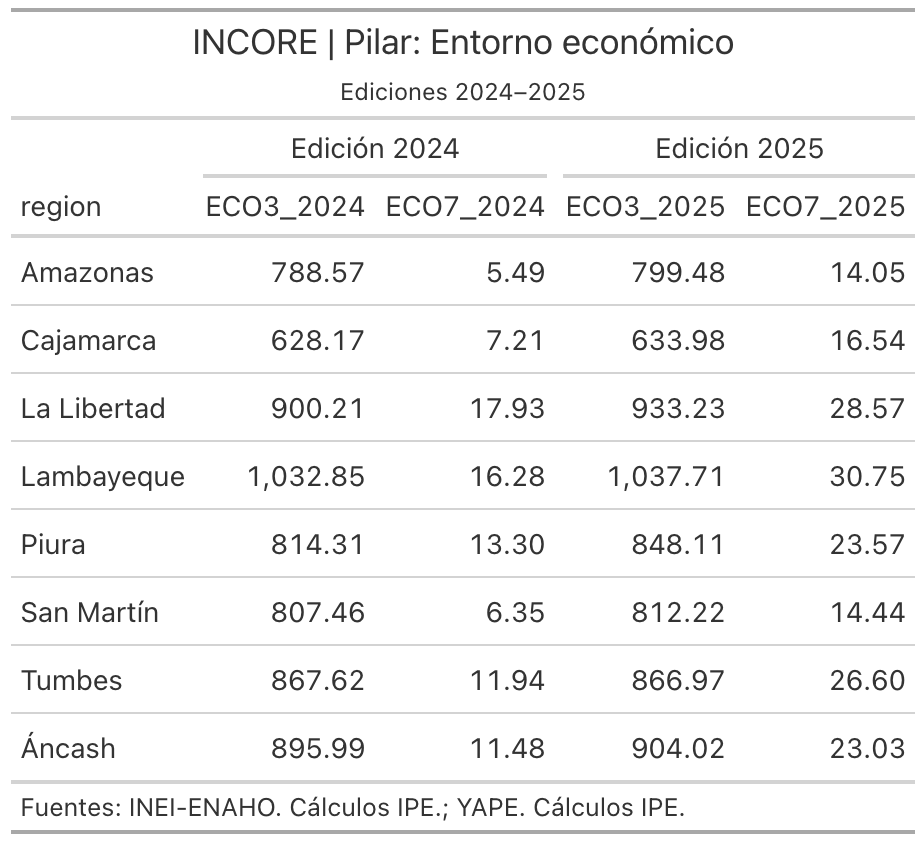
\includegraphics[width=0.9\textwidth,height=\textheight]{tabla.png}
\end{center}

\textbf{Se espera:} resolución que mapea ``3.1 \ldots{}'' a ECO3 (si
aplica en el catálogo) y columnas \textbf{solo} de los indicadores
seleccionados×edición.

\begin{enumerate}
\def\labelenumi{\arabic{enumi}.}
\setcounter{enumi}{3}
\tightlist
\item
  \textbf{Filtrado regional con exclusiones e inclusión de Perú}
\end{enumerate}

\textbf{Se desea lo siguiente:} obtener \textbf{ECO (2025)} solo para
\textbf{Costa} y \textbf{Macro Norte}, \textbf{excluyendo Lima*} e
\textbf{incluyendo Perú}.

\begin{Shaded}
\begin{Highlighting}[]
\NormalTok{val\_reg }\OtherTok{\textless{}{-}} \FunctionTok{valor\_tabla}\NormalTok{(}
  \AttributeTok{ediciones   =} \DecValTok{2025}\NormalTok{,}
  \AttributeTok{pilar       =} \StringTok{"ECO"}\NormalTok{,}
  \AttributeTok{regiones    =} \FunctionTok{c}\NormalTok{(}\StringTok{"gr\_costa"}\NormalTok{, }\StringTok{"gr\_macro\_norte"}\NormalTok{, }\StringTok{"{-}Lima*"}\NormalTok{),}
  \AttributeTok{incluir\_peru =} \ConstantTok{TRUE}
\NormalTok{)}
\NormalTok{val\_reg}
\end{Highlighting}
\end{Shaded}

\begin{verbatim}
# A tibble: 10 x 8
   region  ECO1_2025 ECO2_2025 ECO3_2025 ECO4_2025 ECO5_2025 ECO6_2025 ECO7_2025
   <chr>       <dbl>     <dbl>     <dbl>     <dbl>     <dbl>     <dbl>     <dbl>
 1 Arequi~      4.50      18.3     1074.     42.3       63.9      38.0      25.2
 2 Ica          4.33      23.4     1117.     67.5       62.0      33.5      31.3
 3 La Lib~      4.40      17.4      933.     40.6       52.0      26.8      28.6
 4 Lambay~      4.13      16.1     1038.     15.9       54.5      33.4      30.7
 5 Lima P~      4.28      19.1      871.     18.0       55.7      26.3      36.5
 6 Moqueg~      4.14      25.4     1164.    104.        68.3      35.8      25.7
 7 Piura        4.33      15.9      848.     28.7       50.9      29.7      23.6
 8 Tacna        3.95      15.6      915.     14.5       46.0      34.9      18.5
 9 Tumbes       3.48      15.6      867.      5.71      48.8      30.8      26.6
10 Áncash       4.33      14.7      904.     58.1       49.4      23.9      23.0
\end{verbatim}

\textbf{Se espera:} que aparezca la fila \textbf{``Perú''} y se apliquen
correctamente los \textbf{grupos} y \textbf{exclusiones}.

\begin{enumerate}
\def\labelenumi{\arabic{enumi}.}
\setcounter{enumi}{4}
\tightlist
\item
  \textbf{Salida gt con spanners por edición para reporte}
\end{enumerate}

\textbf{Se desea lo siguiente:} presentar en un informe los
\textbf{valores} de \textbf{LAB3 (2023--2025)} como \textbf{tabla gt}
con encabezados por edición.

\begin{Shaded}
\begin{Highlighting}[]
\NormalTok{val\_gt }\OtherTok{\textless{}{-}} \FunctionTok{valor\_tabla}\NormalTok{(}\AttributeTok{ediciones =} \DecValTok{2022}\SpecialCharTok{:}\DecValTok{2025}\NormalTok{, }
                      \AttributeTok{pilar =} \StringTok{"LAB"}\NormalTok{, }
                      \AttributeTok{indicadores =} \StringTok{"LAB3"}\NormalTok{,}
                      \AttributeTok{gt =} \ConstantTok{TRUE}\NormalTok{)}
\end{Highlighting}
\end{Shaded}

\begin{center}
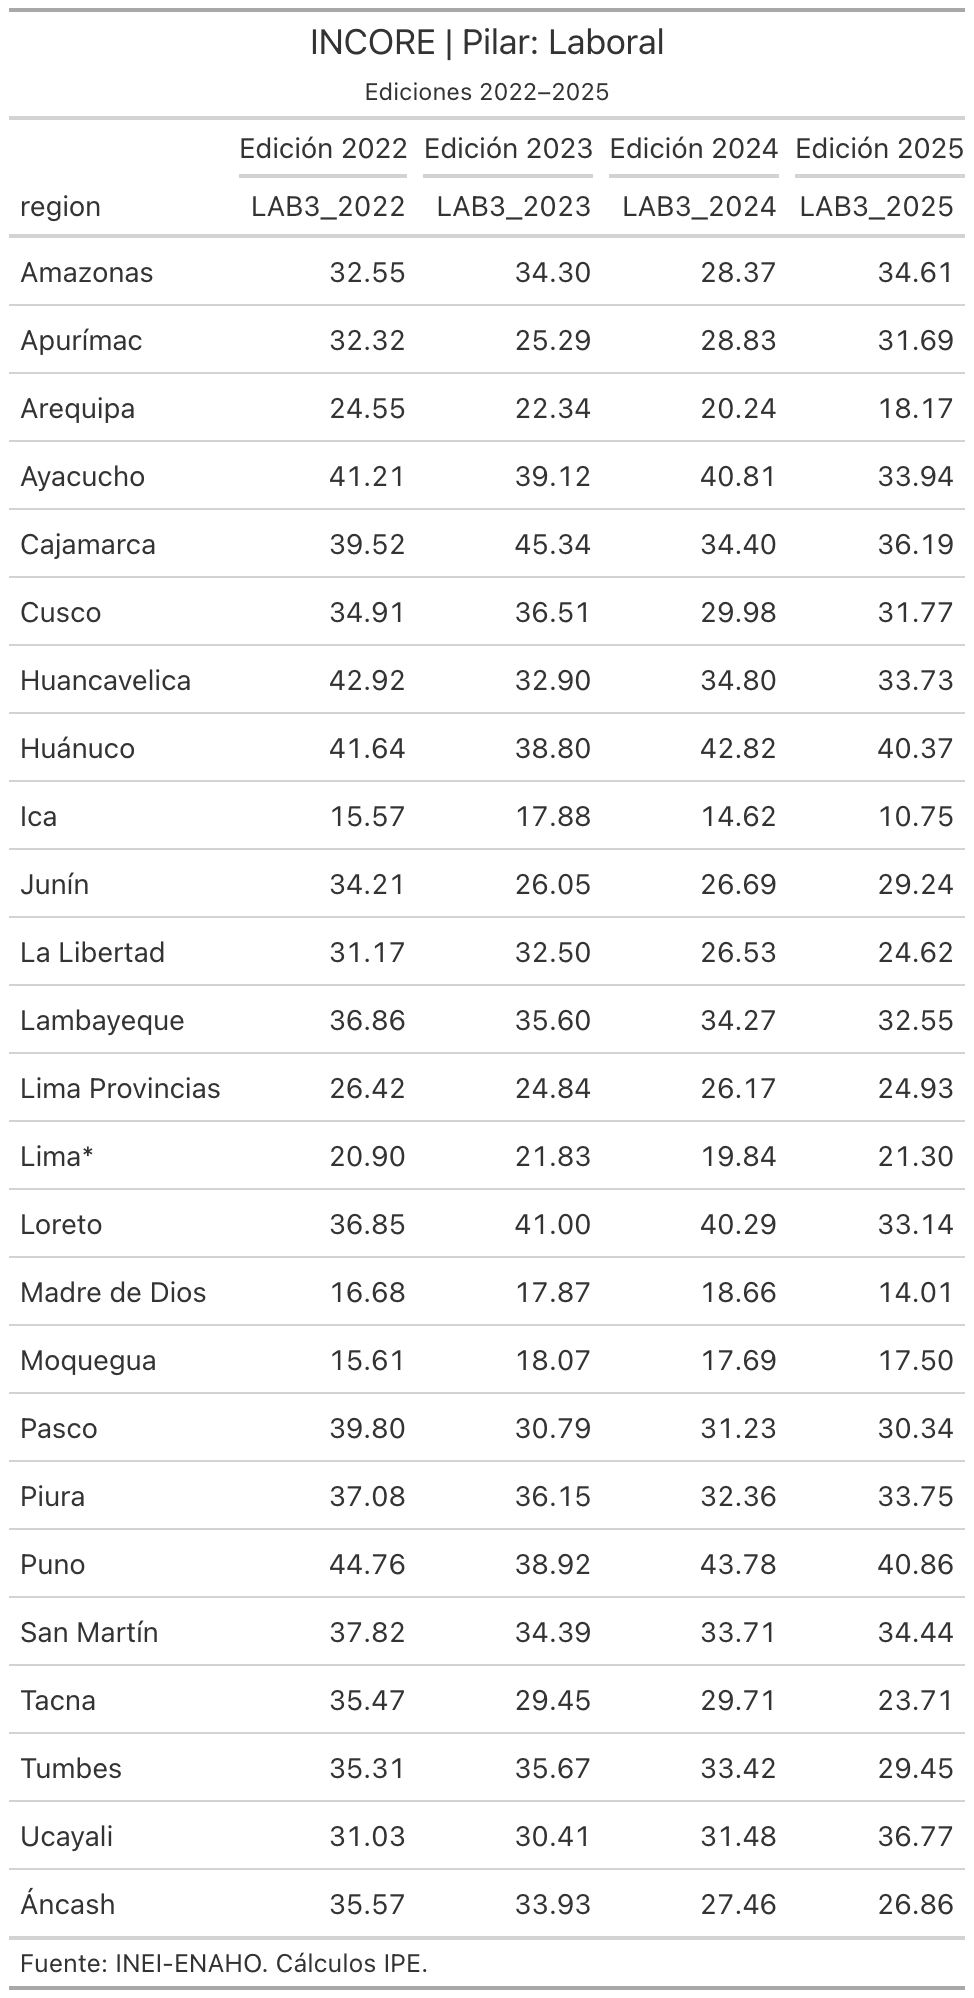
\includegraphics[width=0.9\textwidth,height=\textheight]{vuru.png}
\end{center}

\textbf{Se espera:} una \textbf{tabla gt} con formateo numérico y
\textbf{spanners} por edición (``Edición 2023'', ``Edición 2024'',
``Edición 2025'').

\subsection{\texorpdfstring{\textbf{Barras por región para un
indicador(indc\_barras) y para su valor
(valor\_barras)}}{Barras por región para un indicador(indc\_barras) y para su valor (valor\_barras)}}\label{barras-por-regiuxf3n-para-un-indicadorindc_barras-y-para-su-valor-valor_barras}

\begin{itemize}
\item
  indc\_barras() grafica el \textbf{puntaje (0--10)} del indicador,
  coherente con la escala estandarizada del índice.
\item
  valor\_barras() grafica el \textbf{valor original} del indicador (no
  estandarizado), mostrando en el eje la \textbf{unidad propia} y en el
  \emph{caption} la \textbf{fuente}.
\end{itemize}

\subsubsection{\texorpdfstring{\textbf{Parámetros}}{Parámetros}}\label{paruxe1metros-9}

Para un uso práctico y consistente, conviene definir \textbf{edición},
\textbf{indicador} (por código o nombre) y, cuando sea necesario, el
\textbf{pilar} para desambiguar. El filtrado por regiones admite
\textbf{grupos} gr\_* y \textbf{exclusiones} con prefijo ``-''. En ambos
casos, usar\_codigos (siempre que sea TRUE) facilita traducir códigos a
nombres oficiales \textbf{antes} del filtrado, incluir\_peru añade o no
la fila ``Perú'' (promedio nacional). Estos dos se tratan como
secundarios y no aparecen en las viñetas.

\subsubsection{\texorpdfstring{\textbf{indc\_barras: puntaje (0--10) de
un
indicador}}{indc\_barras: puntaje (0--10) de un indicador}}\label{indc_barras-puntaje-010-de-un-indicador}

\begin{itemize}
\item
  edicion: \textbf{edición} a graficar.

  \begin{itemize}
  \tightlist
  \item
    Opciones válidas: 2016 \ldots{} 2025 (p.ej., 2025).
  \end{itemize}
\item
  pilar: \textbf{pilar} al que pertenece el indicador.

  \begin{itemize}
  \item
    Formatos aceptados: código ``ECO''/``LAB''/\ldots{} o nombre
    ``Entorno económico''/``Laboral''/\ldots{}
  \item
    Puede omitirse si indicador \textbf{identifica unívocamente}.
  \end{itemize}
\item
  indicador: \textbf{indicador} a graficar.

  \begin{itemize}
  \item
    Formatos aceptados: código (p.ej., ``LAB2'') o nombre completo
    (p.ej., ``2.2 Formalidad laboral'').
  \item
    Recomendado \textbf{especificarlo} para evitar ambigüedades.
  \end{itemize}
\item
  regiones: universo de \textbf{regiones} a incluir.

  \begin{itemize}
  \item
    ``ALL'' (todas)
  \item
    Listas por nombre/código (p.ej., c(``Arequipa'',``Cusco'') o
    c(``ARE'',``CUS''))
  \item
    \textbf{Grupos}: ``gr\_costa'', ``gr\_sierra'', ``gr\_selva''
  \item
    \textbf{Exclusiones} por patrón: p.ej., ``-Lima*''
  \item
    Combinables: c(``gr\_costa'',``-Lima*'',``La Libertad'')
  \end{itemize}
\item
  paleta: esquema de color cualitativo por región.

  \begin{itemize}
  \tightlist
  \item
    ``ipe'' (por defecto), ``okabe\_ito'', ``viridis''
  \end{itemize}
\item
  mostrar\_leyenda: control de la leyenda.

  \begin{itemize}
  \tightlist
  \item
    FALSE (por defecto) o TRUE
  \end{itemize}
\end{itemize}

\subsubsection{\texorpdfstring{\textbf{valor\_barras(): valor original
del indicador (no
puntaje)}}{valor\_barras(): valor original del indicador (no puntaje)}}\label{valor_barras-valor-original-del-indicador-no-puntaje}

\begin{itemize}
\item
  edicion: \textbf{edición} a graficar.

  \begin{itemize}
  \tightlist
  \item
    Opciones válidas: 2016 \ldots{} 2025 (p.ej., 2024).
  \end{itemize}
\item
  pilar: \textbf{pilar} del indicador (código o nombre).

  \begin{itemize}
  \tightlist
  \item
    Puede omitirse si indicador \textbf{es único} en la edición/filtro.
  \end{itemize}
\item
  indicador: \textbf{indicador} a graficar.

  \begin{itemize}
  \item
    Código (p.ej., ``ECO7'') o nombre (p.ej., ``1.7 Billeteras
    digitales'').
  \item
    El título puede rotularse por \textbf{código} o \textbf{nombre} con
    label\_indicador.
  \end{itemize}
\item
  regiones: universo de \textbf{regiones} a incluir.

  \begin{itemize}
  \tightlist
  \item
    ``ALL'', listas por nombre/código, \textbf{grupos} gr\_*,
    \textbf{exclusiones} con ``-'' (mismos patrones que arriba).
  \end{itemize}
\item
  paleta: esquema de color cualitativo por región.

  \begin{itemize}
  \tightlist
  \item
    ``ipe'', ``okabe\_ito'', ``viridis''
  \end{itemize}
\item
  mostrar\_leyenda: control de la leyenda.

  \begin{itemize}
  \tightlist
  \item
    FALSE (por defecto) o TRUE
  \end{itemize}
\item
  label\_indicador: cómo \textbf{rotular} el indicador en el título.

  \begin{itemize}
  \tightlist
  \item
    ``nombre'' (por defecto) o ``cod''
  \end{itemize}
\end{itemize}

\subsubsection{\texorpdfstring{\textbf{Explicación
conceptual}}{Explicación conceptual}}\label{explicaciuxf3n-conceptual-11}

Ambas funciones \textbf{leen} la edición indicada, \textbf{normalizan}
cadenas clave y aplican filtros defensivos:

\begin{itemize}
\item
  \texttt{indc\_barras()} retiene \textbf{puntajes 0--10} del indicador
  seleccionado, consolida a \textbf{un valor por región} (promedios
  defensivos ante duplicados), \textbf{ordena} de mayor a menor y
  \textbf{colorea} por región con paletas predefinidas. Es ideal para
  \textbf{ranking} dentro de un indicador concreto.
\item
  \texttt{valor\_barras()} trabaja con la \textbf{magnitud observada}
  del indicador (no el puntaje), respeta la \textbf{unidad} original en
  el eje y añade la \textbf{fuente} como \emph{caption}, con el mismo
  enfoque de \textbf{consolidación} y \textbf{orden}. Permite
  interpretar \textbf{qué significa} una diferencia de valores en
  términos sustantivos (por ejemplo, tasas, montos, porcentajes).
\end{itemize}

\subsubsection{\texorpdfstring{\textbf{Ejemplos}}{Ejemplos}}\label{ejemplos-11}

\paragraph{\texorpdfstring{\textbf{1) Puntaje 0--10 de un indicador por
región
(básico)}}{1) Puntaje 0--10 de un indicador por región (básico)}}\label{puntaje-010-de-un-indicador-por-regiuxf3n-buxe1sico}

\textbf{Se desea lo siguiente:} graficar el \textbf{puntaje} del
indicador (código) en la edición 2025 para \textbf{todas} las regiones.

\begin{Shaded}
\begin{Highlighting}[]
\FunctionTok{indc\_barras}\NormalTok{(}
  \AttributeTok{edicion   =} \DecValTok{2025}\NormalTok{,}
  \AttributeTok{pilar     =} \StringTok{"LAB"}\NormalTok{,}
  \AttributeTok{indicador =} \StringTok{"LAB2"}\NormalTok{,}
  \AttributeTok{regiones  =} \StringTok{"ALL"}\NormalTok{,}
  \AttributeTok{paleta    =} \StringTok{"ipe"}\NormalTok{,}
  \AttributeTok{mostrar\_leyenda =} \ConstantTok{FALSE}
\NormalTok{)}
\end{Highlighting}
\end{Shaded}

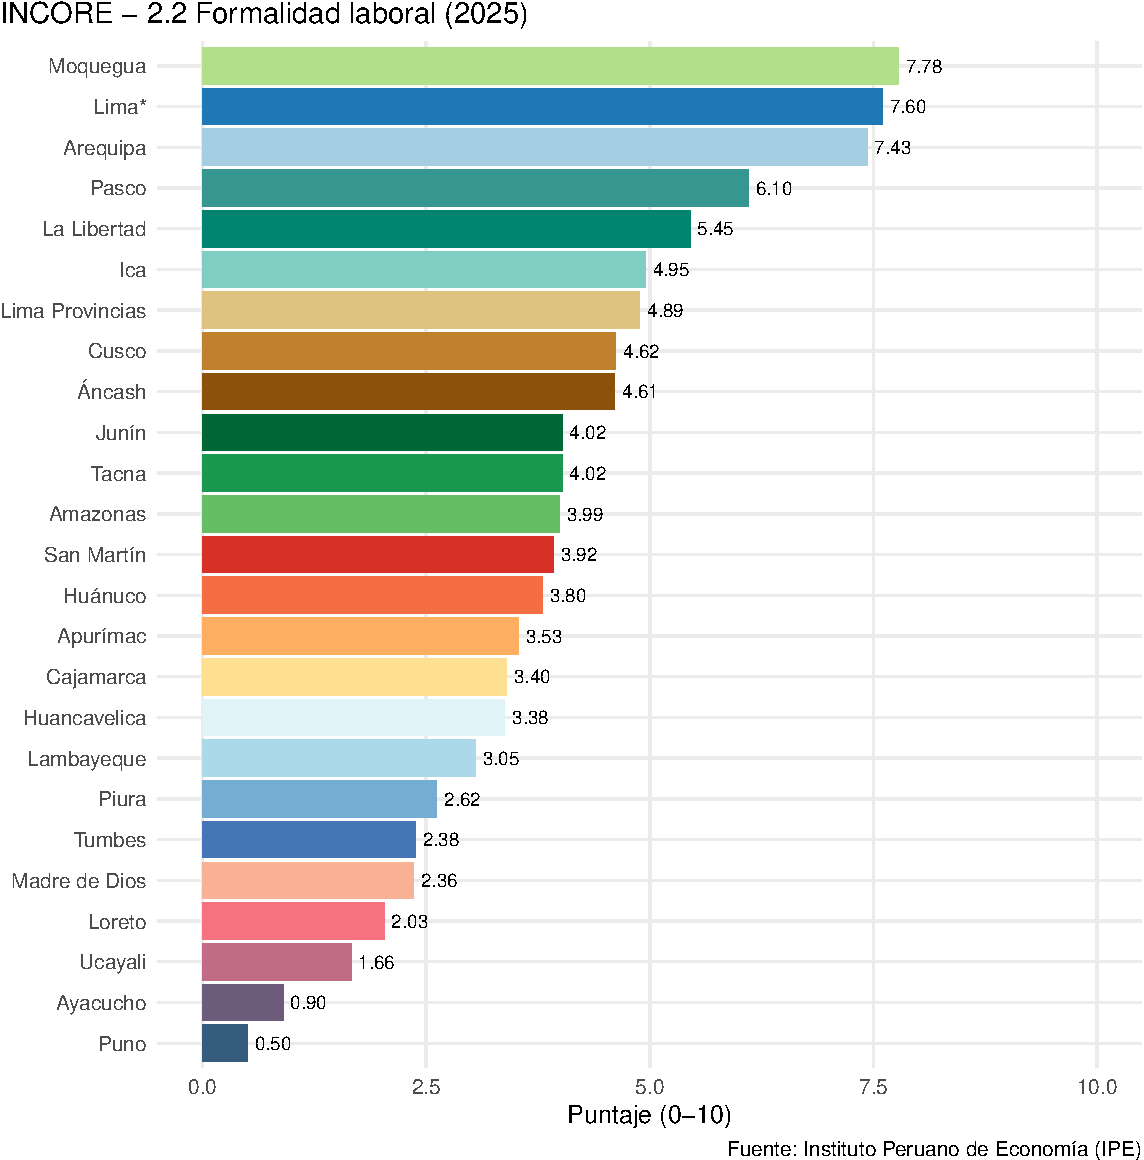
\includegraphics{Manual_files/figure-pdf/unnamed-chunk-73-1.pdf}

\textbf{Resultado esperado.} Barras horizontales ordenadas (0--10), una
por región, con etiquetas de valor y estilo del paquete.

\paragraph{\texorpdfstring{\textbf{2) Puntaje por grupo costero con
exclusión de un
patrón}}{2) Puntaje por grupo costero con exclusión de un patrón}}\label{puntaje-por-grupo-costero-con-exclusiuxf3n-de-un-patruxf3n}

\textbf{Se desea lo siguiente:} comparar el \textbf{puntaje} del
indicador por las \textbf{regiones de la costa}, excluyendo las que
empiecen con ``Lima*''.

\begin{Shaded}
\begin{Highlighting}[]
\FunctionTok{indc\_barras}\NormalTok{(}
  \AttributeTok{edicion   =} \DecValTok{2025}\NormalTok{,}
  \AttributeTok{pilar     =} \StringTok{"ECO"}\NormalTok{,}
  \AttributeTok{indicador =} \StringTok{"ECO7"}\NormalTok{,}
  \AttributeTok{regiones  =} \FunctionTok{c}\NormalTok{(}\StringTok{"gr\_costa"}\NormalTok{, }\StringTok{"{-}Lima*"}\NormalTok{),}
  \AttributeTok{paleta    =} \StringTok{"okabe\_ito"}\NormalTok{,}
  \AttributeTok{mostrar\_leyenda =} \ConstantTok{TRUE}
\NormalTok{)}
\end{Highlighting}
\end{Shaded}

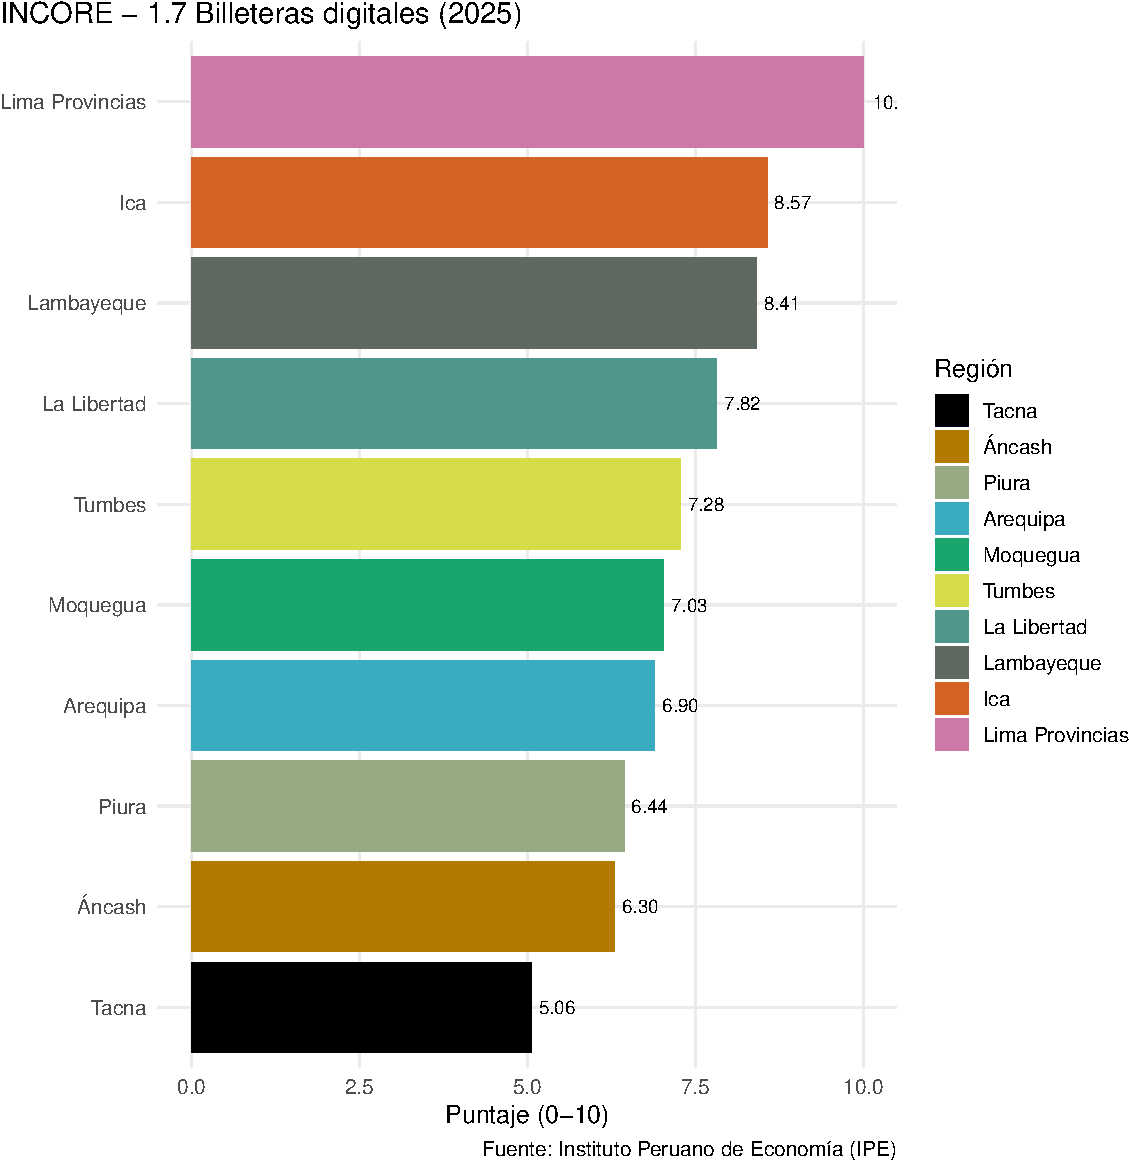
\includegraphics{Manual_files/figure-pdf/unnamed-chunk-74-1.pdf}

\textbf{Resultado esperado.} Barras para el subconjunto costero
\textbf{sin} Lima*, útiles para contrastes regionales enfocados.

\paragraph{\texorpdfstring{\textbf{3) Valor original del indicador con
unidad en el
eje}}{3) Valor original del indicador con unidad en el eje}}\label{valor-original-del-indicador-con-unidad-en-el-eje}

\textbf{Se desea lo siguiente:} graficar el \textbf{valor} del indicador
(no puntaje) para 2024, mostrando la \textbf{unidad} en el eje y la
\textbf{fuente} automática.

\begin{Shaded}
\begin{Highlighting}[]
\FunctionTok{valor\_barras}\NormalTok{(}
  \AttributeTok{edicion   =} \DecValTok{2024}\NormalTok{,}
  \AttributeTok{pilar     =} \StringTok{"ECO"}\NormalTok{,}
  \AttributeTok{indicador =} \StringTok{"ECO7"}\NormalTok{,}
  \AttributeTok{regiones  =} \StringTok{"ALL"}\NormalTok{,}
  \AttributeTok{paleta    =} \StringTok{"ipe"}\NormalTok{,}
  \AttributeTok{mostrar\_leyenda =} \ConstantTok{FALSE}\NormalTok{,}
  \AttributeTok{label\_indicador =} \StringTok{"nombre"}
\NormalTok{)}
\end{Highlighting}
\end{Shaded}

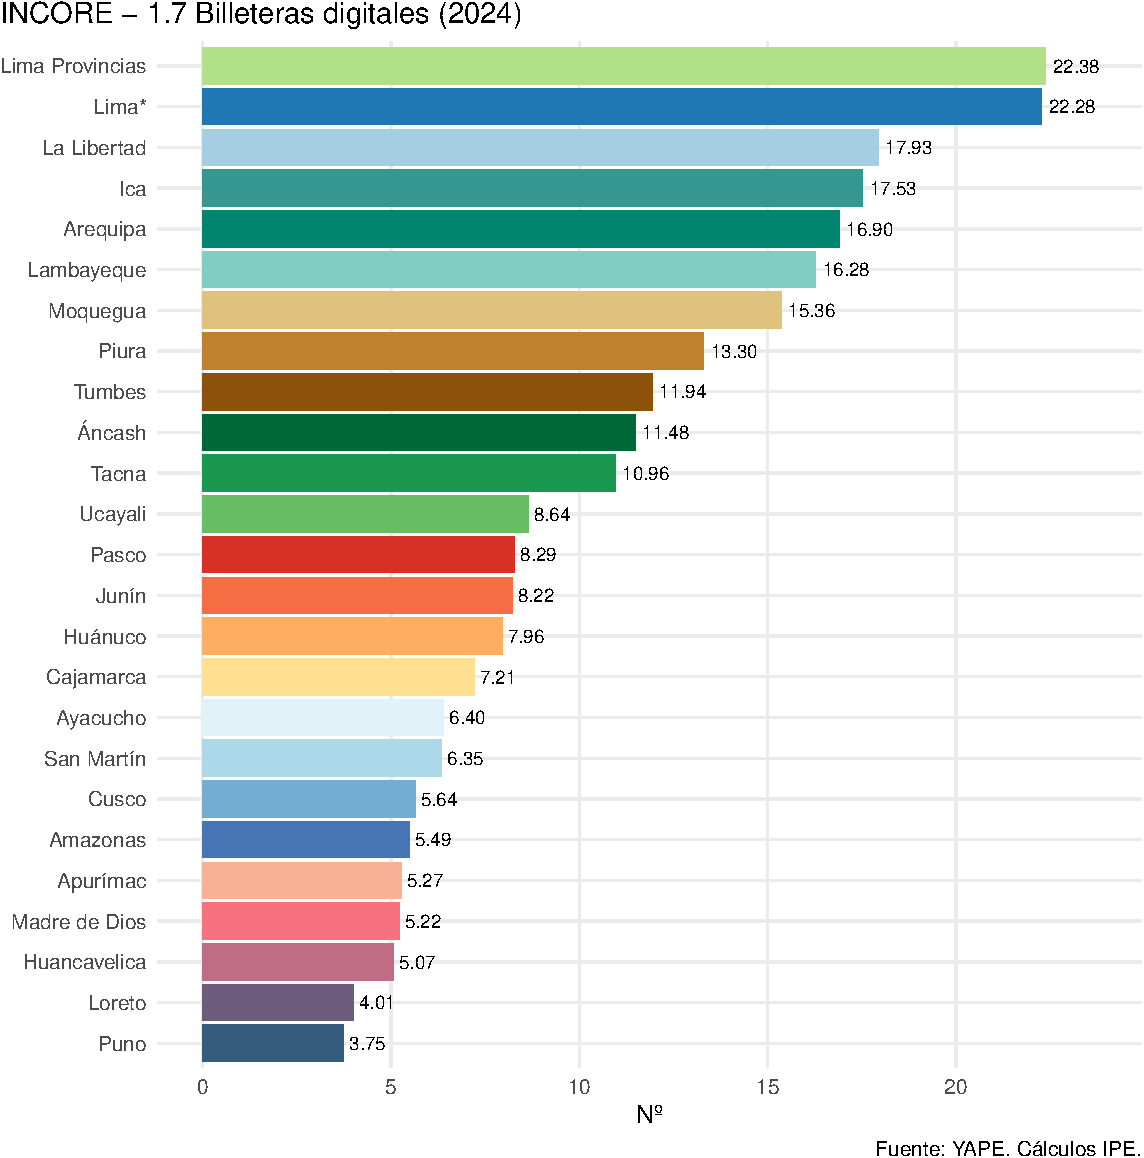
\includegraphics{Manual_files/figure-pdf/unnamed-chunk-75-1.pdf}

\textbf{Resultado esperado.} Barras con eje rotulado según la
\textbf{unidad corta} del indicador, ordenadas de mayor a menor.

\paragraph{\texorpdfstring{\textbf{4) Valor del indicador para un
subconjunto mixto y con
``Perú''}}{4) Valor del indicador para un subconjunto mixto y con ``Perú''}}\label{valor-del-indicador-para-un-subconjunto-mixto-y-con-peruxfa}

\textbf{Se desea lo siguiente:} comparar valores en regiones específicas
\textbf{más} un grupo, \textbf{incluyendo ``Perú''} para referencia.

\begin{Shaded}
\begin{Highlighting}[]
\FunctionTok{valor\_barras}\NormalTok{(}
  \AttributeTok{edicion       =} \DecValTok{2024}\NormalTok{,}
  \AttributeTok{indicador     =} \StringTok{"1.7 Billeteras digitales"}\NormalTok{,}
  \AttributeTok{regiones      =} \FunctionTok{c}\NormalTok{(}\StringTok{"Arequipa"}\NormalTok{, }\StringTok{"La Libertad"}\NormalTok{, }\StringTok{"gr\_sierra"}\NormalTok{),}
  \AttributeTok{incluir\_peru  =} \ConstantTok{TRUE}\NormalTok{,}
  \AttributeTok{paleta        =} \StringTok{"viridis"}\NormalTok{,}
  \AttributeTok{mostrar\_leyenda =} \ConstantTok{TRUE}\NormalTok{,}
  \AttributeTok{label\_indicador =} \StringTok{"cod"}
\NormalTok{)}
\end{Highlighting}
\end{Shaded}

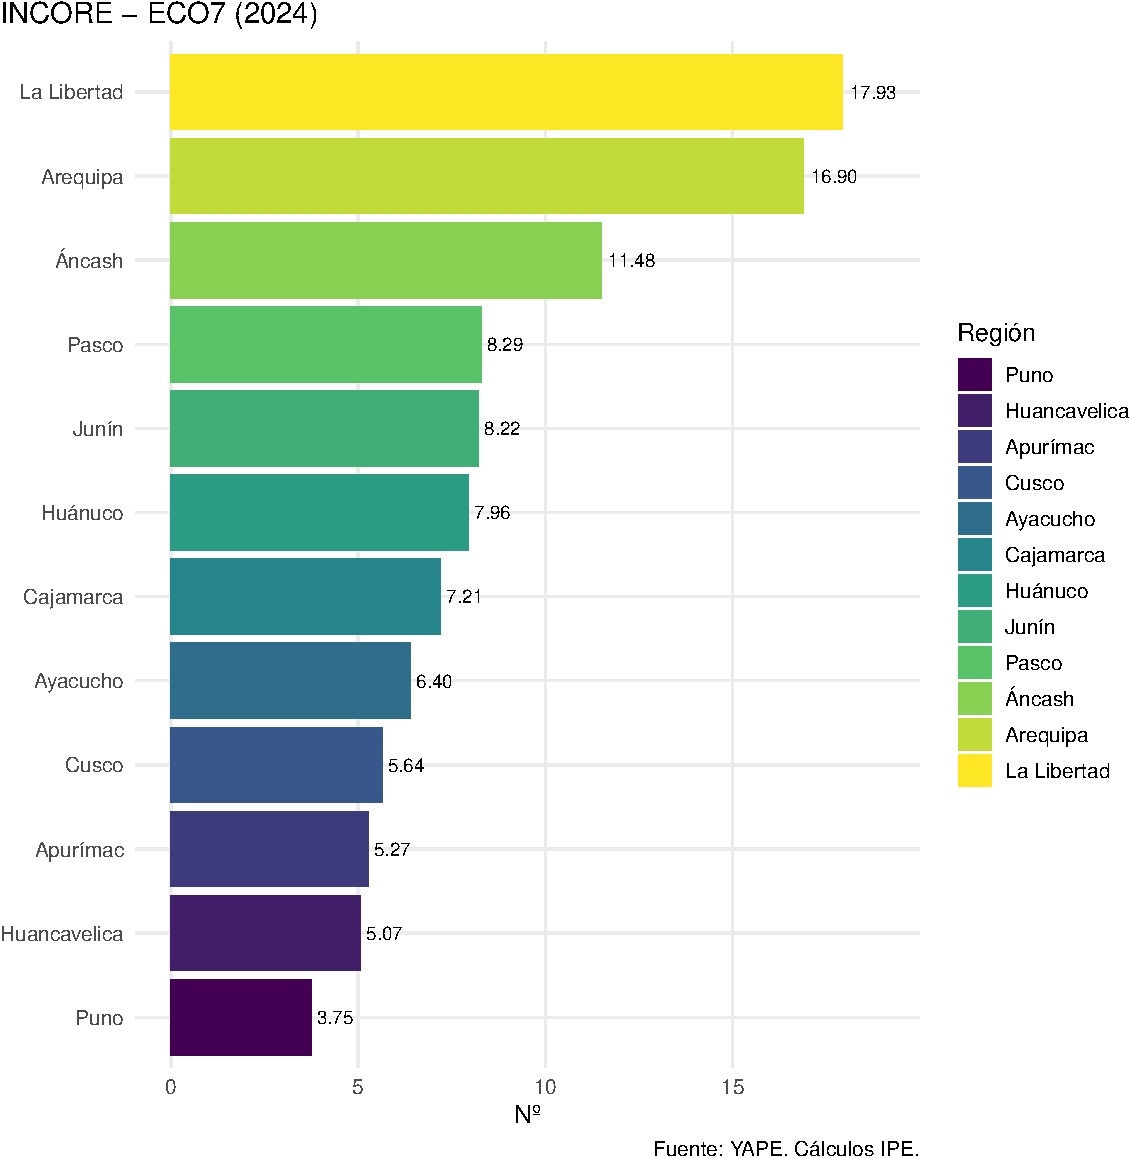
\includegraphics{Manual_files/figure-pdf/unnamed-chunk-76-1.pdf}

\textbf{Resultado esperado.} Barras para el conjunto mixto (regiones
explícitas + grupo), \textbf{con} la fila ``Perú'', paleta continua
cualitativa y rótulo del título por \textbf{código}.

\paragraph{\texorpdfstring{\textbf{5) Puntaje por indicador
identificado}}{5) Puntaje por indicador identificado}}\label{puntaje-por-indicador-identificado}

\begin{Shaded}
\begin{Highlighting}[]
\FunctionTok{indc\_barras}\NormalTok{(}
  \AttributeTok{edicion   =} \DecValTok{2025}\NormalTok{,}
  \AttributeTok{indicador =} \StringTok{"2.2 Formalidad laboral"}\NormalTok{,  }\CommentTok{\# ejemplo de nombre completo}
  \AttributeTok{regiones  =} \FunctionTok{c}\NormalTok{(}\StringTok{"gr\_selva"}\NormalTok{, }\StringTok{"Cusco"}\NormalTok{),}
  \AttributeTok{paleta    =} \StringTok{"ipe"}\NormalTok{,}
  \AttributeTok{mostrar\_leyenda =} \ConstantTok{FALSE}
\NormalTok{)}
\end{Highlighting}
\end{Shaded}

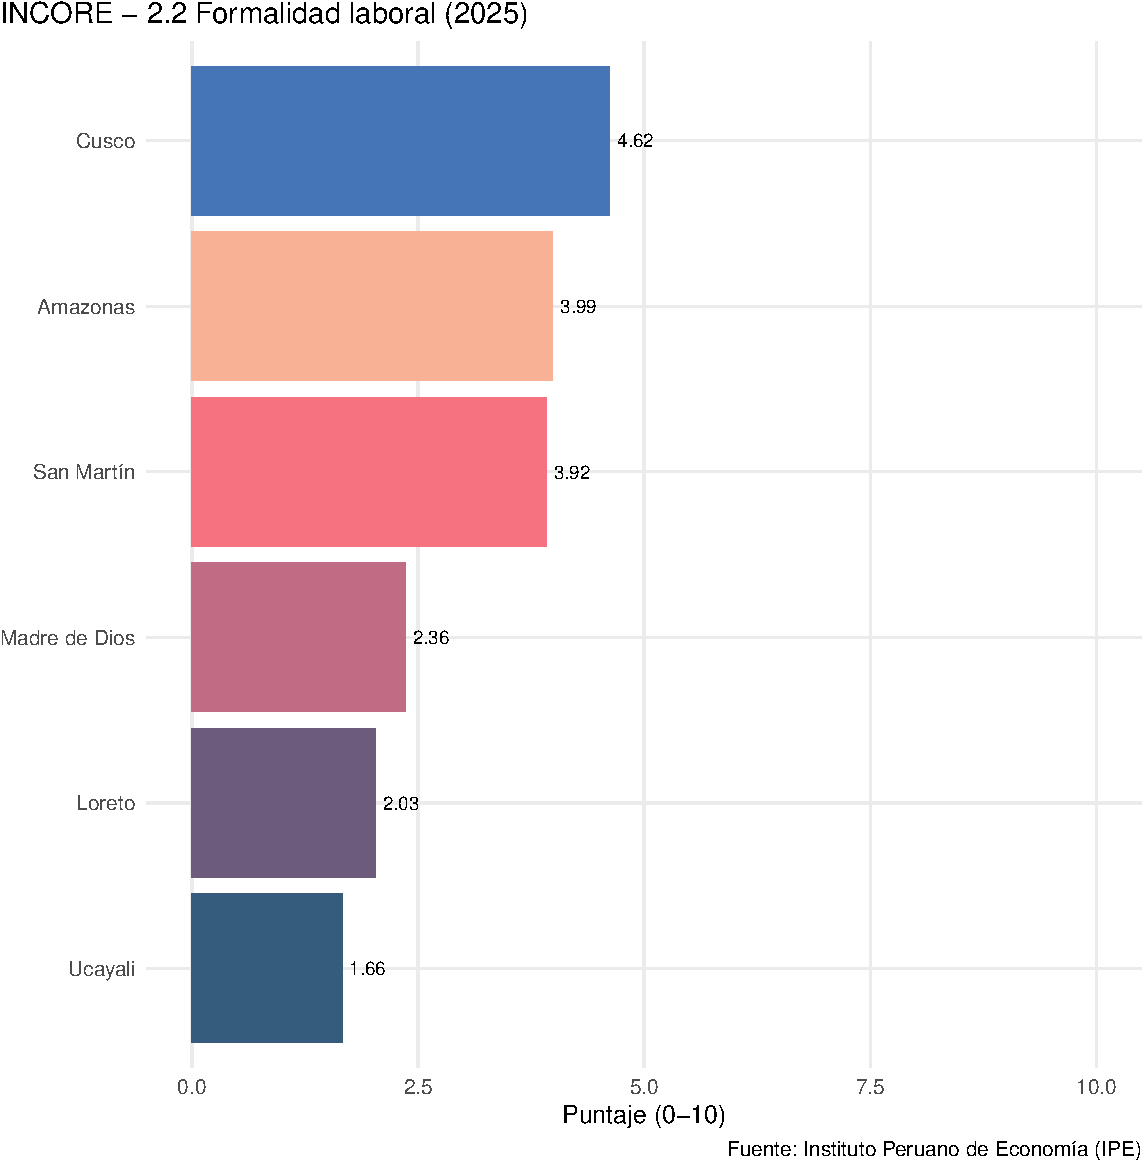
\includegraphics{Manual_files/figure-pdf/unnamed-chunk-77-1.pdf}

\textbf{Resultado esperado.} Barras por región del \textbf{puntaje}
(0--10) para el indicador identificado por \textbf{nombre}, si el nombre
no es único fuera del pilar, el pilar desambiguará correctamente.

\subsection{\texorpdfstring{\textbf{Líneas por indicador (valor\_largo)
y por puntaje
(indc\_largo)}}{Líneas por indicador (valor\_largo) y por puntaje (indc\_largo)}}\label{luxedneas-por-indicador-valor_largo-y-por-puntaje-indc_largo}

\begin{itemize}
\item
  valor\_largo() grafica la \textbf{evolución de valores originales} (no
  puntajes) de uno o varios indicadores de un pilar a lo largo de
  \textbf{múltiples ediciones}. Rotula cada facet con \textbf{código o
  nombre} y añade \textbf{unidad} al panel (cuando se elige por código).
\item
  indc\_largo() grafica la \textbf{evolución del puntaje (0--10)} por
  \textbf{indicador} de un pilar, también en \textbf{varias ediciones},
  con facets por indicador (rotulados por \textbf{nombre} completo o
  \textbf{código}).
\end{itemize}

\subsubsection{\texorpdfstring{\textbf{Parámetros: decisiones
clave}}{Parámetros: decisiones clave}}\label{paruxe1metros-decisiones-clave}

\textbf{Comunes}

\begin{itemize}
\item
  ediciones: rango con \textbf{≥ 2} años (p.ej., 2019:2025).
\item
  pilar: código ``ECO''/``LAB''/\ldots{} o nombre ``Entorno
  económico''/``Laboral''/\ldots.
\item
  indicadores: ``ALL'' o mezcla de \textbf{códigos y nombres}, en
  valor\_largo().
\item
  regiones: ``ALL'', lista de nombres/códigos, y combinaciones con
  \textbf{grupos} gr\_* y \textbf{exclusiones} con ``-''.
\item
  usar\_codigos: si TRUE, traduce códigos \textbf{antes} de filtrar.
\item
  facetear: si TRUE, genera \textbf{facets por indicador}, útil cuando
  hay varios.
\end{itemize}

\textbf{Sólo en valor\_largo()}

\begin{itemize}
\item
  paleta: ``ipe'', ``okabe\_ito'', ``viridis''.
\item
  mostrar\_puntos: puntos sobre las líneas.
\item
  label\_indicador: ``codigo'' (default) o ``nombre'' para el rótulo del
  facet.
\end{itemize}

\textbf{Sólo en indc\_largo()}

\begin{itemize}
\item
  facet\_label\_nombre: TRUE (default) rotula los facets con
  \textbf{``d.d nombre completo''}, FALSE usa el \textbf{código}
  (``EDU3'').
\item
  paleta, mostrar\_puntos: iguales que arriba.
\end{itemize}

\subsubsection{\texorpdfstring{\textbf{Explicación
conceptual}}{Explicación conceptual}}\label{explicaciuxf3n-conceptual-12}

\begin{itemize}
\item
  valor\_largo() trabaja con la \textbf{magnitud observada} (no
  estandarizada). Filtra \textbf{valores ≠ puntaje}, mapea
  \textbf{código↔nombre} con el catálogo y arma \textbf{etiquetas de
  facet} (código o nombre + \textbf{unidad corta}). Ideal para
  interpretar cambios \textbf{sustantivos} (tasas, montos, porcentajes)
  por indicador y región en el tiempo.
\item
  indc\_largo() se limita al \textbf{puntaje 0--10} (estandarizado),
  excluye ``General'' y \textbf{``Perú''} por defecto, y consolida a
  \textbf{un valor por (región, edición, indicador)}. Útil para comparar
  \textbf{trayectorias relativas} entre regiones manteniendo la
  \textbf{misma escala}.
\end{itemize}

\subsubsection{\texorpdfstring{\textbf{Ejemplos}}{Ejemplos}}\label{ejemplos-12}

\paragraph{\texorpdfstring{\textbf{A) Valores originales con
valor\_largo()}}{A) Valores originales con valor\_largo()}}\label{a-valores-originales-con-valor_largo}

\begin{enumerate}
\def\labelenumi{\arabic{enumi}.}
\tightlist
\item
  \textbf{Varios indicadores (auto) en un rango de años}
\end{enumerate}

\textbf{Se desea lo siguiente:} graficar la \textbf{evolución de
valores} de \textbf{todos} los indicadores del pilar ECO (2020--2025)
para \textbf{todas} las regiones, con facets automáticos.

\begin{Shaded}
\begin{Highlighting}[]
\FunctionTok{valor\_largo}\NormalTok{(}
  \AttributeTok{ediciones      =} \DecValTok{2020}\SpecialCharTok{:}\DecValTok{2025}\NormalTok{,}
  \AttributeTok{pilar          =} \StringTok{"ECO"}\NormalTok{,}
  \AttributeTok{indicadores    =} \StringTok{"ALL"}\NormalTok{,}
  \AttributeTok{regiones       =} \StringTok{"ALL"}\NormalTok{,}
  \AttributeTok{facetear       =} \ConstantTok{TRUE}\NormalTok{,}
  \AttributeTok{paleta         =} \StringTok{"ipe"}\NormalTok{,}
  \AttributeTok{mostrar\_puntos =} \ConstantTok{TRUE}\NormalTok{,}
  \AttributeTok{label\_indicador =} \StringTok{"codigo"}
\NormalTok{)}
\end{Highlighting}
\end{Shaded}

\includegraphics{Manual_files/figure-pdf/unnamed-chunk-78-1.pdf}

\textbf{Resultado esperado.} Paneles por indicador (ECO1, ECO2, \ldots)
con líneas por región, el rótulo muestra \textbf{código + unidad}.

\begin{enumerate}
\def\labelenumi{\arabic{enumi}.}
\setcounter{enumi}{1}
\tightlist
\item
  \textbf{Selección mixta de indicadores}
\end{enumerate}

\textbf{Se desea lo siguiente:} graficar sólo \textbf{ECO3} en
2016--2025.

\begin{Shaded}
\begin{Highlighting}[]
\FunctionTok{valor\_largo}\NormalTok{(}
  \AttributeTok{ediciones   =} \DecValTok{2016}\SpecialCharTok{:}\DecValTok{2025}\NormalTok{,}
  \AttributeTok{pilar       =} \StringTok{"ECO"}\NormalTok{,}
  \AttributeTok{indicadores =} \FunctionTok{c}\NormalTok{(}\StringTok{"ECO2"}\NormalTok{),}
  \AttributeTok{regiones    =} \StringTok{"gr\_sur"}\NormalTok{,}
  \AttributeTok{facetear    =} \ConstantTok{TRUE}\NormalTok{,}
  \AttributeTok{paleta      =} \StringTok{"okabe\_ito"}\NormalTok{,}
  \AttributeTok{label\_indicador =} \StringTok{"nombre"}
\NormalTok{)}
\end{Highlighting}
\end{Shaded}

\includegraphics{Manual_files/figure-pdf/unnamed-chunk-79-1.pdf}

\textbf{Resultado esperado.} Facets sólo de los tres indicadores
solicitados, los que empiezan con ``3.1 \ldots{}'' se \textbf{mapean a
ECO3} si corresponde.

\begin{enumerate}
\def\labelenumi{\arabic{enumi}.}
\setcounter{enumi}{2}
\tightlist
\item
  \textbf{Subconjunto regional con exclusiones}
\end{enumerate}

\textbf{Se desea lo siguiente:} graficar valores de \textbf{LAB (ALL)}
en 2019--2025 para la \textbf{Costa} y la \textbf{Macro Norte},
\textbf{excluyendo} ``Lima*''.

\begin{Shaded}
\begin{Highlighting}[]
\FunctionTok{valor\_largo}\NormalTok{(}
  \AttributeTok{ediciones   =} \DecValTok{2019}\SpecialCharTok{:}\DecValTok{2025}\NormalTok{,}
  \AttributeTok{pilar       =} \StringTok{"LAB"}\NormalTok{,}
  \AttributeTok{indicadores =} \StringTok{"ALL"}\NormalTok{,}
  \AttributeTok{regiones    =} \FunctionTok{c}\NormalTok{(}\StringTok{"gr\_costa"}\NormalTok{, }\StringTok{"gr\_norte"}\NormalTok{, }\StringTok{"{-}Lima*"}\NormalTok{),}
  \AttributeTok{paleta      =} \StringTok{"viridis"}\NormalTok{,}
  \AttributeTok{facetear    =} \ConstantTok{TRUE}
\NormalTok{)}
\end{Highlighting}
\end{Shaded}

\includegraphics{Manual_files/figure-pdf/unnamed-chunk-80-1.pdf}

\textbf{Resultado esperado.} Líneas sólo para las regiones filtradas,
Lima* no aparece en los paneles.

\paragraph{\texorpdfstring{\textbf{B) Puntajes 0--10 con
indc\_largo()}}{B) Puntajes 0--10 con indc\_largo()}}\label{b-puntajes-010-con-indc_largo}

\begin{enumerate}
\def\labelenumi{\arabic{enumi}.}
\tightlist
\item
  \textbf{Todos los indicadores de un pilar (puntaje) en varios años}
\end{enumerate}

\textbf{Se desea lo siguiente:} graficar la \textbf{evolución del
puntaje (0--10)} de todos los \textbf{indicadores} del pilar
\textbf{EDU} (2018--2025), por región.

\begin{Shaded}
\begin{Highlighting}[]
\FunctionTok{indc\_largo}\NormalTok{(}
  \AttributeTok{ediciones          =} \DecValTok{2018}\SpecialCharTok{:}\DecValTok{2025}\NormalTok{,}
  \AttributeTok{pilar              =} \StringTok{"EDU"}\NormalTok{,}
  \AttributeTok{indicadores        =} \StringTok{"ALL"}\NormalTok{,}
  \AttributeTok{regiones           =} \StringTok{"gr\_norte"}\NormalTok{,}
  \AttributeTok{facetear           =} \ConstantTok{TRUE}\NormalTok{,}
  \AttributeTok{facet\_label\_nombre =} \ConstantTok{TRUE}\NormalTok{,}
  \AttributeTok{paleta             =} \StringTok{"ipe"}\NormalTok{,}
  \AttributeTok{mostrar\_puntos     =} \ConstantTok{TRUE}
\NormalTok{)}
\end{Highlighting}
\end{Shaded}

\includegraphics{Manual_files/figure-pdf/unnamed-chunk-81-1.pdf}

\begin{enumerate}
\def\labelenumi{\arabic{enumi}.}
\setcounter{enumi}{1}
\tightlist
\item
  \textbf{Lista acotada de indicadores por código y nombre}
\end{enumerate}

\textbf{Se desea lo siguiente:} comparar sólo \textbf{LAB2} y
\textbf{``2.5 \ldots{}''} (por nombre) en 2020--2025.

\begin{Shaded}
\begin{Highlighting}[]
\FunctionTok{indc\_largo}\NormalTok{(}
  \AttributeTok{ediciones          =} \DecValTok{2020}\SpecialCharTok{:}\DecValTok{2025}\NormalTok{,}
  \AttributeTok{pilar              =} \StringTok{"LAB"}\NormalTok{,}
  \AttributeTok{indicadores        =} \FunctionTok{c}\NormalTok{(}\StringTok{"LAB2"}\NormalTok{, }\StringTok{"2.5 Inserción laboral juvenil"}\NormalTok{),}
  \AttributeTok{regiones           =} \StringTok{"ALL"}\NormalTok{,}
  \AttributeTok{facetear           =} \ConstantTok{TRUE}\NormalTok{,}
  \AttributeTok{facet\_label\_nombre =} \ConstantTok{FALSE}\NormalTok{,  }\CommentTok{\# usar rótulo por código}
  \AttributeTok{paleta             =} \StringTok{"okabe\_ito"}
\NormalTok{)}
\end{Highlighting}
\end{Shaded}

\includegraphics{Manual_files/figure-pdf/unnamed-chunk-82-1.pdf}

\textbf{Resultado esperado.} Dos facets (códigos), con líneas de
regiones y escala 0--10.

\begin{enumerate}
\def\labelenumi{\arabic{enumi}.}
\setcounter{enumi}{2}
\tightlist
\item
  \textbf{Con grupos y exclusiones de regiones}
\end{enumerate}

\textbf{Se desea lo siguiente:} puntajes de \textbf{ECO} (indicadores
ALL) en 2023--2025 para \textbf{Sierra} y \textbf{Selva}, excluyendo
``Lima*''.

\begin{Shaded}
\begin{Highlighting}[]
\FunctionTok{indc\_largo}\NormalTok{(}
  \AttributeTok{ediciones   =} \DecValTok{2023}\SpecialCharTok{:}\DecValTok{2025}\NormalTok{,}
  \AttributeTok{pilar       =} \StringTok{"ECO"}\NormalTok{,}
  \AttributeTok{indicadores =} \StringTok{"ALL"}\NormalTok{,}
  \AttributeTok{regiones    =} \FunctionTok{c}\NormalTok{(}\StringTok{"gr\_sur"}\NormalTok{, }\StringTok{"gr\_selva"}\NormalTok{, }\StringTok{"{-}Lima*"}\NormalTok{),}
  \AttributeTok{paleta      =} \StringTok{"viridis"}\NormalTok{,}
  \AttributeTok{facetear    =} \ConstantTok{TRUE}
\NormalTok{)}
\end{Highlighting}
\end{Shaded}

\includegraphics{Manual_files/figure-pdf/unnamed-chunk-83-1.pdf}

\textbf{Resultado esperado.} Facets por indicador, sólo líneas de
regiones pertenecientes a los grupos especificados, sin Lima*.

\subsection{\texorpdfstring{\textbf{Mapas por indicador (valor\_mapa) y
por puntaje
(indc\_mapa)}}{Mapas por indicador (valor\_mapa) y por puntaje (indc\_mapa)}}\label{mapas-por-indicador-valor_mapa-y-por-puntaje-indc_mapa}

\begin{itemize}
\item
  \textbf{valor\_mapa()} colorea cada región por el \textbf{valor
  original} del indicador (no estandarizado). El eje/leyenda usa la
  \textbf{unidad propia} y el \emph{caption} la \textbf{fuente}.
\item
  \textbf{indc\_mapa()} colorea por el \textbf{puntaje (0--10)} del
  indicador, en la misma escala estandarizada del índice.
\end{itemize}

\subsubsection{\texorpdfstring{\textbf{Parámetros: decisiones
clave}}{Parámetros: decisiones clave}}\label{paruxe1metros-decisiones-clave-1}

\textbf{Comunes}

\begin{itemize}
\item
  \textbf{edicion}: un año (2016--2025), p.ej. 2025.
\item
  \textbf{indicador}: código ``ECO3'', ``LAB2''\ldots{} o \textbf{nombre
  completo}.
\item
  \textbf{pilar}: código ``ECO''/``LAB''/\ldots{} o nombre,
  \textbf{opcional} (se usa para validar coherencia).
\item
  \textbf{regiones}: ``ALL'', lista de nombres/códigos y combinaciones
  con \textbf{grupos} gr\_* y \textbf{exclusiones} ``-'' (mismos
  patrones que en otras funciones).
\item
  \textbf{usar\_codigos}: si TRUE, traduce códigos \textbf{antes} de
  filtrar.
\item
  \textbf{mapa\_sf}: objeto sf con region y geometry. Si NULL, se usa
  mapa\_peru(simplificar=\ldots).
\item
  \textbf{simplificar}: tolerancia para mapa\_peru(), 0 = sin
  simplificar.
\item
  \textbf{zoom} y \textbf{expand\_zoom}: acotan la vista al
  \emph{bounding box} de las regiones con datos.
\item
  \textbf{etiquetas}: ``repel'', ``texto'' o ``ninguna'' para rotular
  valores dentro del mapa.
\end{itemize}

\textbf{Sólo en valor\_mapa()}

\begin{itemize}
\item
  \textbf{paleta} (continua): ``blues'' (default), ``viridis'',
  ``cividis'', ``magma''.
\item
  \textbf{subtitulo\_nombre}: TRUE muestra \textbf{nombre} del indicador
  en el subtítulo, FALSE usa el \textbf{código}.
\end{itemize}

\textbf{Sólo en indc\_mapa()}

\begin{itemize}
\item
  \textbf{paleta} (continua): ``blues'', ``greens'', ``viridis'',
  ``cividis'', ``magma'', ``divergente''.
\item
  \textbf{subtitulo\_nombre}: TRUE rotula el subtítulo con
  \textbf{nombre}, FALSE con \textbf{código}.
\end{itemize}

\subsubsection{\texorpdfstring{\textbf{Explicación
conceptual}}{Explicación conceptual}}\label{explicaciuxf3n-conceptual-13}

\begin{itemize}
\item
  \textbf{valor\_mapa()} trabaja con la \textbf{magnitud observada} (no
  estandarizada): filtra valores ≠ ``Puntaje del 0 al 10'', consolida a
  \textbf{un valor por región} (promedio defensivo), usa \textbf{escala
  continua} acorde al rango real del indicador, muestra \textbf{unidad
  completa} en subtítulo y \textbf{unidad corta} en la leyenda, y añade
  \textbf{fuente} en el \emph{caption}.
\item
  \textbf{indc\_mapa()} se limita al \textbf{puntaje 0--10}, excluye
  ``Perú'' y ``General'', consolida por región y aplica paletas
  continuas en el rango {[}0,10{]}. Útil para comparar
  \textbf{posicionamiento relativo} entre regiones con la misma escala
  del índice.
\end{itemize}

\subsubsection{\texorpdfstring{\textbf{Ejemplos}}{Ejemplos}}\label{ejemplos-13}

\paragraph{\texorpdfstring{\textbf{A) Mapas de valores originales con
valor\_mapa()}}{A) Mapas de valores originales con valor\_mapa()}}\label{a-mapas-de-valores-originales-con-valor_mapa}

\begin{enumerate}
\def\labelenumi{\arabic{enumi}.}
\tightlist
\item
  \textbf{Indicador por código, todas las regiones}
\end{enumerate}

\textbf{Se desea lo siguiente:} colorear por el \textbf{valor} de ECO7
en \textbf{2025}, con etiquetas y paleta en azul.

\begin{Shaded}
\begin{Highlighting}[]
\FunctionTok{valor\_mapa}\NormalTok{(}
  \AttributeTok{edicion          =} \DecValTok{2025}\NormalTok{,}
  \AttributeTok{indicador        =} \StringTok{"ECO7"}\NormalTok{,}
  \AttributeTok{regiones         =} \StringTok{"ALL"}\NormalTok{,}
  \AttributeTok{paleta           =} \StringTok{"blues"}\NormalTok{,}
  \AttributeTok{etiquetas        =} \StringTok{"repel"}\NormalTok{,}
  \AttributeTok{subtitulo\_nombre =} \ConstantTok{TRUE}
\NormalTok{)}
\end{Highlighting}
\end{Shaded}

\includegraphics{Manual_files/figure-pdf/unnamed-chunk-84-1.pdf}

\textbf{Resultado esperado.} Coropleta por región con leyenda en
\textbf{unidad propia} (abreviada), subtítulo con nombre completo y
\emph{caption} con la(s) \textbf{fuente(s)}.

\begin{enumerate}
\def\labelenumi{\arabic{enumi}.}
\setcounter{enumi}{1}
\tightlist
\item
  \textbf{Nombre de indicador + zoom a subconjunto regional}
\end{enumerate}

\textbf{Se desea lo siguiente:} mapear el valor de \textbf{``1.7
Billeteras digitales''} en 2024, sólo para \textbf{Costa} y
\textbf{Norte}, excluyendo ``Lima*'', y \textbf{zoom} al área.

\begin{Shaded}
\begin{Highlighting}[]
\FunctionTok{valor\_mapa}\NormalTok{(}
  \AttributeTok{edicion   =} \DecValTok{2024}\NormalTok{,}
  \AttributeTok{indicador =} \StringTok{"1.7 Billeteras digitales"}\NormalTok{,}
  \AttributeTok{regiones  =} \FunctionTok{c}\NormalTok{(}\StringTok{"gr\_costa"}\NormalTok{, }\StringTok{"gr\_norte"}\NormalTok{, }\StringTok{"{-}Lima*"}\NormalTok{),}
  \AttributeTok{paleta    =} \StringTok{"viridis"}\NormalTok{,}
  \AttributeTok{etiquetas =} \StringTok{"texto"}\NormalTok{,}
  \AttributeTok{zoom      =} \ConstantTok{TRUE}
\NormalTok{)}
\end{Highlighting}
\end{Shaded}

\includegraphics{Manual_files/figure-pdf/unnamed-chunk-85-1.pdf}

\textbf{Resultado esperado.} Mapa enfocado al subconjunto con etiquetas
simples y leyenda continua en la unidad correspondiente.

\paragraph{\texorpdfstring{\textbf{B) Mapas de puntajes 0--10 con
indc\_mapa()}}{B) Mapas de puntajes 0--10 con indc\_mapa()}}\label{b-mapas-de-puntajes-010-con-indc_mapa}

\begin{enumerate}
\def\labelenumi{\arabic{enumi}.}
\tightlist
\item
  \textbf{Indicador por código, paleta continua}
\end{enumerate}

\textbf{Se desea lo siguiente:} colorear por el \textbf{puntaje} de LAB2
en 2025 para \textbf{todas} las regiones.

\begin{Shaded}
\begin{Highlighting}[]
\FunctionTok{indc\_mapa}\NormalTok{(}
  \AttributeTok{edicion          =} \DecValTok{2025}\NormalTok{,}
  \AttributeTok{indicador        =} \StringTok{"LAB2"}\NormalTok{,}
  \AttributeTok{regiones         =} \StringTok{"ALL"}\NormalTok{,}
  \AttributeTok{paleta           =} \StringTok{"greens"}\NormalTok{,}
  \AttributeTok{etiquetas        =} \StringTok{"repel"}\NormalTok{,}
  \AttributeTok{subtitulo\_nombre =} \ConstantTok{FALSE}  \CommentTok{\# subtítulo con código}
\NormalTok{)}
\end{Highlighting}
\end{Shaded}

\includegraphics{Manual_files/figure-pdf/unnamed-chunk-86-1.pdf}

\textbf{Resultado esperado.} Coropleta en escala 0--10, subtítulo con
\textbf{código}, etiquetas numéricas redondeadas.

\begin{enumerate}
\def\labelenumi{\arabic{enumi}.}
\setcounter{enumi}{1}
\tightlist
\item
  \textbf{Indicador por nombre, con exclusiones y paleta alternativa}
\end{enumerate}

\textbf{Se desea lo siguiente:} puntaje del indicador \textbf{``2.2
Formalidad laboral''} en 2025, sólo \textbf{Selva}.

\begin{Shaded}
\begin{Highlighting}[]
\FunctionTok{indc\_mapa}\NormalTok{(}
  \AttributeTok{edicion   =} \DecValTok{2025}\NormalTok{,}
  \AttributeTok{indicador =} \StringTok{"2.2 Formalidad laboral"}\NormalTok{,}
  \AttributeTok{regiones  =} \FunctionTok{c}\NormalTok{(}\StringTok{"gr\_selva"}\NormalTok{, }\StringTok{"{-}Lima*"}\NormalTok{),}
  \AttributeTok{paleta    =} \StringTok{"cividis"}\NormalTok{,}
  \AttributeTok{etiquetas =} \StringTok{"ninguna"}\NormalTok{,}
  \AttributeTok{zoom      =} \ConstantTok{TRUE}
\NormalTok{)}
\end{Highlighting}
\end{Shaded}

\includegraphics{Manual_files/figure-pdf/unnamed-chunk-87-1.pdf}

\textbf{Resultado esperado.} Mapa con escala 0--10 y vista recortada al
subconjunto, sin etiquetas sobre el mapa.

\subsection{\texorpdfstring{\textbf{Dispersión por indicador
(indc\_dispersion)}}{Dispersión por indicador (indc\_dispersion)}}\label{dispersiuxf3n-por-indicador-indc_dispersion}

\begin{itemize}
\item
  indc\_dispersion() muestra, para \textbf{una edición} y un
  \textbf{pilar}, un diagrama de \textbf{dispersión} donde el eje X son
  los \textbf{códigos de indicadores} (p.ej., LAB2, LAB5, \ldots) y cada
  punto es el \textbf{puntaje (0--10)} de una \textbf{región} en ese
  indicador.
\item
  Filtra siempre a unidad == ``Puntaje del 0 al 10'', excluye
  ``General'' y, por defecto, \textbf{no} incluye ``Perú''.
\end{itemize}

\subsubsection{\texorpdfstring{\textbf{Parámetros: decisiones
clave}}{Parámetros: decisiones clave}}\label{paruxe1metros-decisiones-clave-2}

\textbf{Comunes}

\begin{itemize}
\item
  \textbf{edicion}: año único (2016--2025).
\item
  \textbf{pilar}: código ``ECO''/``LAB''/\ldots{} o nombre ``Entorno
  económico''/``Laboral''/\ldots.
\item
  \textbf{regiones}: ``ALL'', lista de nombres/códigos, y combinaciones
  con \textbf{grupos} gr\_* y \textbf{exclusiones} con ``-'' (p.ej.,
  c(``gr\_costa'',``-Lima*'')).
\item
  \textbf{usar\_codigos}: si TRUE, traduce códigos antes de filtrar.
\item
  \textbf{paleta}: ``ipe'', ``okabe\_ito'', ``viridis''.
\item
  \textbf{mostrar\_leyenda}: muestra/oculta la leyenda por región.
\end{itemize}

\textbf{Promedio y dispersión}

\begin{itemize}
\item
  \textbf{mostrar\_promedio}: si TRUE, agrega un \textbf{rombo} por
  indicador con el \textbf{promedio} regional.
\item
  \textbf{promedio\_shape / promedio\_size / promedio\_color /
  promedio\_fill}: estilo del rombo.
\item
  \textbf{jitter\_width / jitter\_height}: ``apertura''
  horizontal/vertical de los puntos (útil para evitar solapes).
\end{itemize}

\subsubsection{\texorpdfstring{\textbf{Explicación
conceptual}}{Explicación conceptual}}\label{explicaciuxf3n-conceptual-14}

La función consolida a \textbf{un valor por (región × indicador)}
(promedio defensivo si hubiera duplicados), ordena el eje X por
\textbf{código de indicador} y colorea por \textbf{región}. El rombo
opcional indica la \textbf{posición promedio} por indicador, lo cual
facilita ver \textbf{dispersión} y \textbf{asimetrías} entre regiones
sobre la \textbf{misma escala (0--10)}.

\subsubsection{\texorpdfstring{\textbf{Ejemplos}}{Ejemplos}}\label{ejemplos-14}

\paragraph{\texorpdfstring{\textbf{1) Dispersión básica por pilar para
todas las
regiones}}{1) Dispersión básica por pilar para todas las regiones}}\label{dispersiuxf3n-buxe1sica-por-pilar-para-todas-las-regiones}

\textbf{Se desea lo siguiente:} ver la dispersión de puntajes de
\textbf{LAB} en \textbf{2025}, con promedio por indicador.

\begin{Shaded}
\begin{Highlighting}[]
\FunctionTok{indc\_dispersion}\NormalTok{(}
  \AttributeTok{edicion          =} \DecValTok{2025}\NormalTok{,}
  \AttributeTok{pilar            =} \StringTok{"LAB"}\NormalTok{,}
  \AttributeTok{regiones         =} \StringTok{"ALL"}\NormalTok{,}
  \AttributeTok{paleta           =} \StringTok{"ipe"}\NormalTok{,}
  \AttributeTok{mostrar\_promedio =} \ConstantTok{TRUE}
\NormalTok{)}
\end{Highlighting}
\end{Shaded}

\includegraphics{Manual_files/figure-pdf/unnamed-chunk-88-1.pdf}

\textbf{Resultado esperado.} Eje X con LAB1, LAB2, \ldots, puntos por
región y rombos de promedio, eje Y en 0--10.

\paragraph{\texorpdfstring{\textbf{2) Con grupos y exclusiones de
regiones, resaltando
promedio}}{2) Con grupos y exclusiones de regiones, resaltando promedio}}\label{con-grupos-y-exclusiones-de-regiones-resaltando-promedio}

\textbf{Se desea lo siguiente:} comparar \textbf{ECO (2025)} sólo para
\textbf{Costa} y \textbf{Selva}, excluyendo ``Lima*'', mantener el rombo
de promedio.

\begin{Shaded}
\begin{Highlighting}[]
\FunctionTok{indc\_dispersion}\NormalTok{(}
  \AttributeTok{edicion          =} \DecValTok{2025}\NormalTok{,}
  \AttributeTok{pilar            =} \StringTok{"ECO"}\NormalTok{,}
  \AttributeTok{regiones         =} \FunctionTok{c}\NormalTok{(}\StringTok{"gr\_costa"}\NormalTok{, }\StringTok{"gr\_selva"}\NormalTok{, }\StringTok{"{-}Lima*"}\NormalTok{),}
  \AttributeTok{paleta           =} \StringTok{"okabe\_ito"}\NormalTok{,}
  \AttributeTok{mostrar\_promedio =} \ConstantTok{TRUE}\NormalTok{,}
  \AttributeTok{mostrar\_leyenda  =} \ConstantTok{TRUE}
\NormalTok{)}
\end{Highlighting}
\end{Shaded}

\includegraphics{Manual_files/figure-pdf/unnamed-chunk-89-1.pdf}

\textbf{Resultado esperado.} Puntos únicamente de las regiones
filtradas, Lima* no aparece, rombos por indicador.

\paragraph{\texorpdfstring{\textbf{3) Sin promedio, controlando el
jitter y ocultando
leyenda}}{3) Sin promedio, controlando el jitter y ocultando leyenda}}\label{sin-promedio-controlando-el-jitter-y-ocultando-leyenda}

\textbf{Se desea lo siguiente:} para \textbf{EDU (2024)}, ocultar la
leyenda, suprimir el promedio y ajustar la dispersión para evitar
solapes.

\begin{Shaded}
\begin{Highlighting}[]
\FunctionTok{indc\_dispersion}\NormalTok{(}
  \AttributeTok{edicion          =} \DecValTok{2024}\NormalTok{,}
  \AttributeTok{pilar            =} \StringTok{"EDU"}\NormalTok{,}
  \AttributeTok{regiones         =} \StringTok{"ALL"}\NormalTok{,}
  \AttributeTok{paleta           =} \StringTok{"viridis"}\NormalTok{,}
  \AttributeTok{mostrar\_promedio =} \ConstantTok{FALSE}\NormalTok{,}
  \AttributeTok{jitter\_width     =} \FloatTok{0.12}\NormalTok{,}
  \AttributeTok{jitter\_height    =} \FloatTok{0.00}\NormalTok{,}
  \AttributeTok{mostrar\_leyenda  =} \ConstantTok{FALSE}
\NormalTok{)}
\end{Highlighting}
\end{Shaded}

\includegraphics{Manual_files/figure-pdf/unnamed-chunk-90-1.pdf}

\textbf{Resultado esperado.} Nube de puntos por región en cada EDU*, sin
rombos, con mejor separación horizontal.

\subsection{\texorpdfstring{\textbf{Distribución por indicador
(indc\_distribucion)}}{Distribución por indicador (indc\_distribucion)}}\label{distribuciuxf3n-por-indicador-indc_distribucion}

\begin{itemize}
\item
  indc\_distribucion() muestra, para \textbf{una edición} y \textbf{un
  pilar}, la \textbf{distribución de puntajes (0--10)} por
  \textbf{indicador} entre regiones, como \textbf{boxplot} o
  \textbf{violin}. El eje X son \textbf{códigos} (p.ej., LAB1, LAB2,
  \ldots), el eje Y es el \textbf{puntaje (0--10)}.
\item
  Siempre excluye ``Perú'' y ``General'', y consolida a \textbf{un valor
  por (región, indicador)} mediante promedio defensivo si hubiera
  duplicados.
\end{itemize}

\subsubsection{\texorpdfstring{\textbf{Parámetros: decisiones
clave}}{Parámetros: decisiones clave}}\label{paruxe1metros-decisiones-clave-3}

\begin{itemize}
\item
  \textbf{edicion}: año único (p.ej., 2025).
\item
  \textbf{pilar}: código ``ECO''/``LAB''/\ldots{} o nombre ``Entorno
  económico''/``Laboral''/\ldots.
\item
  \textbf{indicadores}: ``ALL'' (default) o vector de
  \textbf{códigos}/\textbf{nombres} (p.ej., c(``LAB1'',``Inserción
  laboral juvenil'')).
\item
  \textbf{regiones}: ``ALL'' o vector, admite \textbf{grupos} gr\_* y
  \textbf{exclusiones} con ``-'' (a través de los helpers de regiones de
  tu paquete).
\item
  \textbf{usar\_codigos}: si TRUE (default), permite pasar códigos en
  pilar/regiones/indicadores.
\item
  \textbf{tipo}: ``boxplot'' (default) o ``violin''.
\item
  \textbf{jitter}: TRUE para superponer puntos individuales (ruido
  controlado).
\item
  \textbf{paleta}: ``blues'' (default), ``viridis'', ``cividis'' ---
  aplicada \textbf{por indicador}.
\item
  \textbf{linea\_promedio}: TRUE dibuja línea horizontal con el
  \textbf{promedio global} de puntajes.
\item
  \textbf{mostrar\_leyenda}: FALSE (default). Útil activarla si quieres
  identificar el \textbf{relleno por indicador}.
\end{itemize}

\subsubsection{\texorpdfstring{\textbf{Explicación
conceptual}}{Explicación conceptual}}\label{explicaciuxf3n-conceptual-15}

\begin{itemize}
\item
  La función trabaja solo con \textbf{puntajes estandarizados (0--10)}
  del INCORE, y \textbf{facilita comparar dispersión} entre regiones por
  indicador dentro del pilar.
\item
  El \textbf{orden} de los indicadores en el eje X se define por la
  \textbf{mediana} de su distribución (desc), lo que ayuda a leer de
  mayor a menor desempeño típico.
\item
  Con tipo = ``boxplot'' ves mediana, IQR y valores atípicos, con tipo =
  ``violin'' ves densidad. El jitter aporta granularidad por región.
\item
  La \textbf{línea punteada} (linea\_promedio) resume el nivel
  \textbf{promedio general} de puntajes.
\end{itemize}

\subsubsection{\texorpdfstring{\textbf{Ejemplos}}{Ejemplos}}\label{ejemplos-15}

\paragraph{\texorpdfstring{\textbf{1) Boxplot de todos los indicadores
de un
pilar}}{1) Boxplot de todos los indicadores de un pilar}}\label{boxplot-de-todos-los-indicadores-de-un-pilar}

\textbf{Se desea lo siguiente:} comparar la \textbf{distribución} de
puntajes de \textbf{LAB} en \textbf{2025} para \textbf{todas} las
regiones.

\begin{Shaded}
\begin{Highlighting}[]
\FunctionTok{indc\_distribucion}\NormalTok{(}
  \AttributeTok{edicion         =} \DecValTok{2025}\NormalTok{,}
  \AttributeTok{pilar           =} \StringTok{"LAB"}\NormalTok{,}
  \AttributeTok{indicadores     =} \StringTok{"ALL"}\NormalTok{,}
  \AttributeTok{regiones        =} \StringTok{"ALL"}\NormalTok{,}
  \AttributeTok{tipo            =} \StringTok{"boxplot"}\NormalTok{,}
  \AttributeTok{jitter          =} \ConstantTok{TRUE}\NormalTok{,}
  \AttributeTok{paleta          =} \StringTok{"blues"}\NormalTok{,}
  \AttributeTok{linea\_promedio  =} \ConstantTok{TRUE}\NormalTok{,}
  \AttributeTok{mostrar\_leyenda =} \ConstantTok{FALSE}
\NormalTok{)}
\end{Highlighting}
\end{Shaded}

\includegraphics{Manual_files/figure-pdf/unnamed-chunk-91-1.pdf}

\textbf{Resultado esperado.} Boxplots por \textbf{LAB1, LAB2, \ldots{}}
ordenados por mediana (desc), con puntos de regiones y línea de promedio
global.

\paragraph{\texorpdfstring{\textbf{2) Violin para un subconjunto de
indicadores}}{2) Violin para un subconjunto de indicadores}}\label{violin-para-un-subconjunto-de-indicadores}

\textbf{Se desea lo siguiente:} visualizar solo \textbf{LAB2} y
\textbf{LAB5} como violines, con puntos, en 2025.

\begin{Shaded}
\begin{Highlighting}[]
\FunctionTok{indc\_distribucion}\NormalTok{(}
  \AttributeTok{edicion         =} \DecValTok{2025}\NormalTok{,}
  \AttributeTok{pilar           =} \StringTok{"LAB"}\NormalTok{,}
  \AttributeTok{indicadores     =} \FunctionTok{c}\NormalTok{(}\StringTok{"LAB2"}\NormalTok{, }\StringTok{"LAB5"}\NormalTok{),}
  \AttributeTok{regiones        =} \StringTok{"ALL"}\NormalTok{,}
  \AttributeTok{tipo            =} \StringTok{"violin"}\NormalTok{,}
  \AttributeTok{jitter          =} \ConstantTok{TRUE}\NormalTok{,}
  \AttributeTok{paleta          =} \StringTok{"viridis"}\NormalTok{,}
  \AttributeTok{linea\_promedio  =} \ConstantTok{TRUE}\NormalTok{,}
  \AttributeTok{mostrar\_leyenda =} \ConstantTok{TRUE}
\NormalTok{)}
\end{Highlighting}
\end{Shaded}

\includegraphics{Manual_files/figure-pdf/unnamed-chunk-92-1.pdf}

\textbf{Resultado esperado.} Dos violines (LAB2, LAB5) con escala 0--10
y línea de promedio.

\paragraph{\texorpdfstring{\textbf{3) Con grupos y exclusiones de
regiones}}{3) Con grupos y exclusiones de regiones}}\label{con-grupos-y-exclusiones-de-regiones}

\textbf{Se desea lo siguiente:} comparar la distribución de \textbf{ECO}
(todos los indicadores) en 2024 para \textbf{Costa} y \textbf{Norte},
excluyendo ``Lima*''.

\begin{Shaded}
\begin{Highlighting}[]
\FunctionTok{indc\_distribucion}\NormalTok{(}
  \AttributeTok{edicion         =} \DecValTok{2024}\NormalTok{,}
  \AttributeTok{pilar           =} \StringTok{"ECO"}\NormalTok{,}
  \AttributeTok{indicadores     =} \StringTok{"ALL"}\NormalTok{,}
  \AttributeTok{regiones        =} \FunctionTok{c}\NormalTok{(}\StringTok{"gr\_costa"}\NormalTok{, }\StringTok{"gr\_norte"}\NormalTok{, }\StringTok{"{-}Lima*"}\NormalTok{),}
  \AttributeTok{tipo            =} \StringTok{"boxplot"}\NormalTok{,}
  \AttributeTok{jitter          =} \ConstantTok{TRUE}\NormalTok{,}
  \AttributeTok{paleta          =} \StringTok{"cividis"}\NormalTok{,}
  \AttributeTok{linea\_promedio  =} \ConstantTok{TRUE}
\NormalTok{)}
\end{Highlighting}
\end{Shaded}

\includegraphics{Manual_files/figure-pdf/unnamed-chunk-93-1.pdf}

\textbf{Resultado esperado.} Distribuciones por indicador solo para las
regiones filtradas, Lima* no aparece.

\subsection{\texorpdfstring{\textbf{Telaraña por INDICADORES
(indc\_radar)}}{Telaraña por INDICADORES (indc\_radar)}}\label{telarauxf1a-por-indicadores-indc_radar}

\begin{itemize}
\item
  indc\_radar() dibuja un \textbf{radar} con los \textbf{indicadores} de
  un \textbf{pilar} en \textbf{una edición}, comparando una o varias
  \textbf{regiones}.
\item
  Los ejes pueden rotularse por \textbf{código} (LAB2, EDU5, \ldots) o
  por \textbf{nombre} completo.
\item
  Siempre usa \textbf{puntaje (0--10)}, excluye ``Perú'' y ``General'',
  y consolida un único valor por (región, indicador).
\end{itemize}

\subsubsection{\texorpdfstring{\textbf{Parámetros}}{Parámetros}}\label{paruxe1metros-10}

\begin{itemize}
\item
  \textbf{edicion}: año a graficar (2016 \ldots{} 2025).
\item
  \textbf{pilar}: código ``ECO''/``LAB''/\ldots{} o nombre ``Entorno
  económico''/``Laboral''/\ldots.
\item
  \textbf{indicadores}: ``ALL'' (default) o vector mixto de
  \textbf{códigos} y/o \textbf{nombres} a incluir.
\item
  \textbf{regiones}:

  \begin{itemize}
  \item
    ``AUTO3'' (default) selecciona automáticamente \textbf{3} regiones
    (baja, media y alta) por promedio del pilar.
  \item
    ``ALL'' o vector de nombres/códigos, admite combinaciones con tus
    \emph{helpers} (grupos/ exclusiones) si prefieres filtrar antes y
    pasar el resultado.
  \end{itemize}
\item
  \textbf{usar\_codigos}: si TRUE, traduce códigos antes de filtrar.
\item
  \textbf{etiquetas\_indicadores}: ``codigo'' (default) o ``nombre''
  para el \textbf{rótulo de ejes}.
\item
  \textbf{max\_regiones}: umbral de advertencia por legibilidad (default
  6).
\item
  \textbf{alpha}: transparencia del \textbf{relleno} (default 0.25).
\item
  \textbf{paleta}: ``ipe'', ``okabe\_ito'', ``viridis'' (cualitativas
  por región).
\item
  \textbf{mostrar\_puntos}: TRUE/FALSE para puntos en los vértices.
\end{itemize}

\subsubsection{\texorpdfstring{\textbf{Explicación
conceptual}}{Explicación conceptual}}\label{explicaciuxf3n-conceptual-16}

El radar compara regiones \textbf{en la misma escala 0--10} para todos
los \textbf{indicadores} del pilar.

\begin{itemize}
\item
  Cuando regiones=``AUTO3'', se eligen automáticamente tres casos
  representativos (bajo/medio/alto) para una lectura rápida.
\item
  Si hay muchos polígonos (muchas regiones), la superposición reduce la
  claridad, por eso se \textbf{advierte} cuando superas max\_regiones.
\item
  Se normaliza/depura para asegurar \textbf{un valor por (región,
  indicador)}, y se recorta a {[}0,10{]} por robustez.
\end{itemize}

\subsubsection{\texorpdfstring{\textbf{Ejemplos}}{Ejemplos}}\label{ejemplos-16}

\paragraph{\texorpdfstring{\textbf{1) Comparación rápida con selección
automática de
regiones}}{1) Comparación rápida con selección automática de regiones}}\label{comparaciuxf3n-ruxe1pida-con-selecciuxf3n-automuxe1tica-de-regiones}

\textbf{Se desea lo siguiente:} un radar de \textbf{Laboral} en
\textbf{2025} con todos los indicadores, dejando que el algoritmo elija
3 regiones representativas.

\begin{Shaded}
\begin{Highlighting}[]
\FunctionTok{indc\_radar}\NormalTok{(}
  \AttributeTok{edicion   =} \DecValTok{2025}\NormalTok{,}
  \AttributeTok{pilar     =} \StringTok{"LAB"}\NormalTok{,}
  \AttributeTok{indicadores =} \StringTok{"ALL"}\NormalTok{,}
  \AttributeTok{regiones  =} \StringTok{"AUTO3"}\NormalTok{,}
  \AttributeTok{etiquetas\_indicadores =} \StringTok{"codigo"}\NormalTok{,  }\CommentTok{\# ejes tipo LAB1, LAB2, ...}
  \AttributeTok{paleta    =} \StringTok{"ipe"}\NormalTok{,}
  \AttributeTok{alpha     =} \FloatTok{0.25}\NormalTok{,}
  \AttributeTok{mostrar\_puntos =} \ConstantTok{TRUE}
\NormalTok{)}
\end{Highlighting}
\end{Shaded}

\includegraphics{Manual_files/figure-pdf/unnamed-chunk-94-1.pdf}

\textbf{Resultado esperado.} Tres polígonos (baja/mediana/alta) con ejes
por \textbf{código} de indicador y escala 0--10.

\paragraph{\texorpdfstring{\textbf{2) Comparar un conjunto específico de
regiones con ejes por
nombre}}{2) Comparar un conjunto específico de regiones con ejes por nombre}}\label{comparar-un-conjunto-especuxedfico-de-regiones-con-ejes-por-nombre}

\textbf{Se desea lo siguiente:} comparar \textbf{Arequipa},
\textbf{Cusco} y \textbf{La Libertad} en \textbf{ECO (2025)}, con ejes
rotulados por \textbf{nombre} de indicador.

\begin{Shaded}
\begin{Highlighting}[]
\FunctionTok{indc\_radar}\NormalTok{(}
  \AttributeTok{edicion   =} \DecValTok{2025}\NormalTok{,}
  \AttributeTok{pilar     =} \StringTok{"EDU"}\NormalTok{,}
  \AttributeTok{indicadores =} \StringTok{"ALL"}\NormalTok{,}
  \AttributeTok{regiones  =} \FunctionTok{c}\NormalTok{(}\StringTok{"Arequipa"}\NormalTok{, }\StringTok{"Cusco"}\NormalTok{, }\StringTok{"La Libertad"}\NormalTok{),}
  \AttributeTok{etiquetas\_indicadores =} \StringTok{"nombre"}\NormalTok{,}
  \AttributeTok{paleta    =} \StringTok{"okabe\_ito"}\NormalTok{,}
  \AttributeTok{alpha     =} \FloatTok{0.3}
\NormalTok{)}
\end{Highlighting}
\end{Shaded}

\includegraphics{Manual_files/figure-pdf/unnamed-chunk-95-1.pdf}

\textbf{Resultado esperado.} Radar con \textbf{3 regiones} y ejes por
\textbf{nombre} completo, título y caption con estilo del paquete.

\paragraph{\texorpdfstring{\textbf{3) Foco en un subconjunto de
indicadores}}{3) Foco en un subconjunto de indicadores}}\label{foco-en-un-subconjunto-de-indicadores}

\textbf{Se desea lo siguiente:} telaraña de \textbf{LAB (2025)} con
\textbf{sólo tres indicadores} (por código o nombre) y un conjunto
amplio de regiones.

\begin{Shaded}
\begin{Highlighting}[]
\FunctionTok{indc\_radar}\NormalTok{(}
  \AttributeTok{edicion   =} \DecValTok{2025}\NormalTok{,}
  \AttributeTok{pilar     =} \StringTok{"LAB"}\NormalTok{,}
  \AttributeTok{indicadores =} \FunctionTok{c}\NormalTok{(}\StringTok{"LAB1"}\NormalTok{, }\StringTok{"LAB2"}\NormalTok{, }\StringTok{"LAB3"}\NormalTok{, }\StringTok{"LAB5"}\NormalTok{, }\StringTok{"LAB6"}\NormalTok{),}
  \AttributeTok{regiones  =} \StringTok{"gr\_norte"}\NormalTok{,}
  \AttributeTok{etiquetas\_indicadores =} \StringTok{"codigo"}\NormalTok{,}
  \AttributeTok{paleta    =} \StringTok{"viridis"}\NormalTok{,}
  \AttributeTok{max\_regiones =} \DecValTok{8}\NormalTok{,  }
  \AttributeTok{alpha     =} \FloatTok{0.2}
\NormalTok{)}
\end{Highlighting}
\end{Shaded}

\includegraphics{Manual_files/figure-pdf/unnamed-chunk-96-1.pdf}

\textbf{Resultado esperado.} Radar con \textbf{sólo los indicadores}
elegidos.

\subsection{\texorpdfstring{\textbf{Distribución por indicador
(indc\_distribucion)}}{Distribución por indicador (indc\_distribucion)}}\label{distribuciuxf3n-por-indicador-indc_distribucion-1}

\begin{itemize}
\item
  \textbf{indc\_distribucion()} muestra, para \textbf{una edición} y
  \textbf{un pilar}, la \textbf{distribución de puntajes (0--10)} por
  \textbf{indicador} entre regiones, como \textbf{boxplot} o
  \textbf{violin}. El eje X son \textbf{códigos} (p.ej., LAB1, LAB2,
  \ldots) y el eje Y es el \textbf{puntaje (0--10)}.
\item
  Siempre \textbf{excluye} ``Perú'' y ``General'', y consolida a
  \textbf{un valor por (región, indicador)} mediante promedio defensivo
  ante duplicados. Internamente lee con agregar\_codigos = TRUE para
  garantizar el eje en códigos.
\end{itemize}

\subsubsection{\texorpdfstring{\textbf{Parámetros: decisiones
clave}}{Parámetros: decisiones clave}}\label{paruxe1metros-decisiones-clave-4}

\begin{itemize}
\item
  \textbf{edicion}: año único (p.ej., 2025).
\item
  \textbf{pilar}: código ``ECO''/``LAB''/\ldots{} o nombre ``Entorno
  económico''/``Laboral''/\ldots.
\item
  \textbf{indicadores}: ``ALL'' (default) o vector de
  \textbf{códigos}/\textbf{nombres} (p.ej., c(``LAB1'',``Inserción
  laboral juvenil'')).
\item
  \textbf{regiones}: ``ALL'' o vector; admite \textbf{grupos} gr\_* y
  \textbf{exclusiones} con ``-'' (vía helpers de regiones).
\item
  \textbf{usar\_codigos}: si TRUE (default), permite pasar códigos en
  pilar/regiones/indicadores.
\item
  \textbf{tipo}: ``boxplot'' (default) o ``violin''.
\item
  \textbf{jitter}: TRUE para superponer puntos individuales (ruido
  controlado).
\item
  \textbf{paleta}: ``blues'' (default), ``viridis'', ``cividis'' ---
  aplicada \textbf{por indicador}.
\item
  \textbf{linea\_promedio}: TRUE dibuja línea horizontal con el
  \textbf{promedio global} de puntajes.
\item
  \textbf{mostrar\_leyenda}: FALSE (default). Útil activarla si quieres
  identificar el \textbf{relleno por indicador}.
\end{itemize}

\subsubsection{\texorpdfstring{\textbf{Explicación
conceptual}}{Explicación conceptual}}\label{explicaciuxf3n-conceptual-17}

\begin{itemize}
\item
  Trabaja solo con \textbf{puntajes estandarizados (0--10)} del INCORE y
  permite comparar \textbf{dispersión} entre regiones por indicador
  dentro del pilar.
\item
  El \textbf{orden} de los indicadores en el eje X se define por la
  \textbf{mediana} de su distribución (desc), facilitando la lectura de
  mayor a menor desempeño típico.
\item
  Con tipo = ``boxplot'' ves mediana, IQR y atípicos; con tipo =
  ``violin'' ves densidad. El jitter aporta la granularidad por región.
\item
  La \textbf{línea punteada} (linea\_promedio) resume el
  \textbf{promedio general} de puntajes de todos los indicadores
  seleccionados.
\end{itemize}

\subsubsection{\texorpdfstring{\textbf{Ejemplos}}{Ejemplos}}\label{ejemplos-17}

\paragraph{\texorpdfstring{\textbf{1) Boxplot de todos los indicadores
de un
pilar}}{1) Boxplot de todos los indicadores de un pilar}}\label{boxplot-de-todos-los-indicadores-de-un-pilar-1}

\textbf{Se desea lo siguiente:} comparar la \textbf{distribución} de
puntajes de \textbf{LAB} en \textbf{2025} para \textbf{todas} las
regiones.

\begin{Shaded}
\begin{Highlighting}[]
\FunctionTok{indc\_distribucion}\NormalTok{(}
  \AttributeTok{edicion         =} \DecValTok{2025}\NormalTok{,}
  \AttributeTok{pilar           =} \StringTok{"LAB"}\NormalTok{,}
  \AttributeTok{indicadores     =} \StringTok{"ALL"}\NormalTok{,}
  \AttributeTok{regiones        =} \StringTok{"ALL"}\NormalTok{,}
  \AttributeTok{tipo            =} \StringTok{"boxplot"}\NormalTok{,}
  \AttributeTok{jitter          =} \ConstantTok{TRUE}\NormalTok{,}
  \AttributeTok{paleta          =} \StringTok{"blues"}\NormalTok{,}
  \AttributeTok{linea\_promedio  =} \ConstantTok{TRUE}\NormalTok{,}
  \AttributeTok{mostrar\_leyenda =} \ConstantTok{FALSE}
\NormalTok{)}
\end{Highlighting}
\end{Shaded}

\includegraphics{Manual_files/figure-pdf/unnamed-chunk-97-1.pdf}

\textbf{Resultado esperado.} Boxplots por \textbf{LAB1, LAB2, \ldots{}}
ordenados por mediana (desc), con puntos por región y una línea de
promedio global.

\paragraph{\texorpdfstring{\textbf{2) Violin para un subconjunto de
indicadores}}{2) Violin para un subconjunto de indicadores}}\label{violin-para-un-subconjunto-de-indicadores-1}

\textbf{Se desea lo siguiente:} visualizar solo \textbf{LAB2} y
\textbf{LAB5} como violines, con puntos, en 2025.

\begin{Shaded}
\begin{Highlighting}[]
\FunctionTok{indc\_distribucion}\NormalTok{(}
  \AttributeTok{edicion         =} \DecValTok{2025}\NormalTok{,}
  \AttributeTok{pilar           =} \StringTok{"LAB"}\NormalTok{,}
  \AttributeTok{indicadores     =} \FunctionTok{c}\NormalTok{(}\StringTok{"LAB2"}\NormalTok{, }\StringTok{"LAB5"}\NormalTok{),}
  \AttributeTok{regiones        =} \StringTok{"ALL"}\NormalTok{,}
  \AttributeTok{tipo            =} \StringTok{"violin"}\NormalTok{,}
  \AttributeTok{jitter          =} \ConstantTok{TRUE}\NormalTok{,}
  \AttributeTok{paleta          =} \StringTok{"viridis"}\NormalTok{,}
  \AttributeTok{linea\_promedio  =} \ConstantTok{TRUE}\NormalTok{,}
  \AttributeTok{mostrar\_leyenda =} \ConstantTok{TRUE}
\NormalTok{)}
\end{Highlighting}
\end{Shaded}

\includegraphics{Manual_files/figure-pdf/unnamed-chunk-98-1.pdf}

\textbf{Resultado esperado.} Dos violines (LAB2, LAB5) con escala 0--10
y línea de promedio.

\paragraph{\texorpdfstring{\textbf{3) Con grupos y exclusiones de
regiones}}{3) Con grupos y exclusiones de regiones}}\label{con-grupos-y-exclusiones-de-regiones-1}

\textbf{Se desea lo siguiente:} comparar la distribución de \textbf{ECO}
(todos los indicadores) en 2024 para \textbf{Costa} y \textbf{Norte},
excluyendo ``Lima*''.

\begin{Shaded}
\begin{Highlighting}[]
\FunctionTok{indc\_distribucion}\NormalTok{(}
  \AttributeTok{edicion         =} \DecValTok{2024}\NormalTok{,}
  \AttributeTok{pilar           =} \StringTok{"ECO"}\NormalTok{,}
  \AttributeTok{indicadores     =} \StringTok{"ALL"}\NormalTok{,}
  \AttributeTok{regiones        =} \FunctionTok{c}\NormalTok{(}\StringTok{"gr\_costa"}\NormalTok{, }\StringTok{"gr\_norte"}\NormalTok{, }\StringTok{"{-}Lima*"}\NormalTok{),}
  \AttributeTok{tipo            =} \StringTok{"boxplot"}\NormalTok{,}
  \AttributeTok{jitter          =} \ConstantTok{TRUE}\NormalTok{,}
  \AttributeTok{paleta          =} \StringTok{"cividis"}\NormalTok{,}
  \AttributeTok{linea\_promedio  =} \ConstantTok{TRUE}
\NormalTok{)}
\end{Highlighting}
\end{Shaded}

\includegraphics{Manual_files/figure-pdf/unnamed-chunk-99-1.pdf}

\textbf{Resultado esperado.} Distribuciones por indicador solo para las
regiones filtradas; ``Lima*'' no aparece.

\subsection{\texorpdfstring{\textbf{Heatmap por indicadores o por tiempo
(indc\_heatmap)}}{Heatmap por indicadores o por tiempo (indc\_heatmap)}}\label{heatmap-por-indicadores-o-por-tiempo-indc_heatmap}

\begin{itemize}
\item
  \textbf{indc\_heatmap()} dibuja un mapa de calor con filas =
  \textbf{regiones} y columnas que pueden ser:

  \begin{itemize}
  \item
    \textbf{Indicadores} de un \textbf{pilar} en \textbf{una} edición
    (modo = ``indicadores'').
  \item
    \textbf{Ediciones} para \textbf{un} \textbf{indicador} (modo =
    ``tiempo'').
  \end{itemize}
\item
  Siempre trabaja con \textbf{puntajes 0--10}, usando
  indc\_leer\_incore(\ldots, agregar\_codigos = TRUE) y excluyendo el
  indicador \textbf{``General''} (y la fila \textbf{``Perú''}).
\end{itemize}

\subsubsection{\texorpdfstring{\textbf{Parámetros: decisiones
clave}}{Parámetros: decisiones clave}}\label{paruxe1metros-decisiones-clave-5}

\begin{itemize}
\item
  \textbf{modo}: ``indicadores'' (columnas = indicadores, una edición) o
  ``tiempo'' (columnas = ediciones, un indicador).
\item
  \textbf{pilar}: código ``ECO''/``LAB''/\ldots{} o nombre ``Entorno
  económico''/``Laboral''/\ldots{} (requerido si modo=``indicadores'').
\item
  \textbf{indicador}: código o nombre (requerido si modo=``tiempo'').
\item
  \textbf{edicion}: año único (cuando modo=``indicadores'').
\item
  \textbf{ediciones}: rango con ≥2 años (cuando modo=``tiempo'', p.ej.,
  2019:2025).
\item
  \textbf{regiones}: ``ALL'' o vector; admite \textbf{grupos} gr\_* y
  \textbf{exclusiones} con ``-'' (se apoya en tus helpers de regiones).
\item
  \textbf{usar\_codigos}: si TRUE, permite pasar códigos en
  pilar/indicador/regiones.
\item
  \textbf{ordenar} (solo modo=``tiempo''): ``ninguno'', ``por\_ultimo''
  (ordena por el valor en la última edición), ``por\_promedio''.
\item
  \textbf{paleta}: ``blues'', ``viridis'', ``cividis'', ``magma''
  (escala continua).
\item
  \textbf{anotar}: si TRUE, escribe el valor dentro de cada celda.
\item
  \textbf{mostrar\_leyenda}: TRUE/FALSE.
\end{itemize}

\subsubsection{\texorpdfstring{\textbf{Explicación
conceptual}}{Explicación conceptual}}\label{explicaciuxf3n-conceptual-18}

\begin{itemize}
\item
  En modo = ``indicadores'' las columnas son \textbf{códigos de
  indicador} (p.ej., LAB1, LAB2, \ldots) del pilar elegido en la
  \textbf{edición} indicada; útil para comparar desempeño \textbf{entre
  indicadores} dentro del pilar.
\item
  En modo = ``tiempo'' las columnas son \textbf{ediciones} para un
  \textbf{indicador} específico; útil para ver \textbf{trayectorias} por
  región.

  El parámetro ordenar ayuda a resaltar patrones (por el último dato o
  por el promedio).
\item
  Siempre se consolida a \textbf{un valor por celda} mediante
  \textbf{promedio defensivo} si aparecen duplicados en (región,
  indicador) o (región, edición).
\end{itemize}

\subsubsection{\texorpdfstring{\textbf{Ejemplos}}{Ejemplos}}\label{ejemplos-18}

\paragraph{\texorpdfstring{\textbf{A) Indicadores de un pilar en una
edición}}{A) Indicadores de un pilar en una edición}}\label{a-indicadores-de-un-pilar-en-una-ediciuxf3n}

\textbf{Se desea lo siguiente:} heatmap de \textbf{EDU} en \textbf{2025}
(todas las regiones), con valores anotados.

\begin{Shaded}
\begin{Highlighting}[]
\FunctionTok{indc\_heatmap}\NormalTok{(}
  \AttributeTok{modo       =} \StringTok{"indicadores"}\NormalTok{,}
  \AttributeTok{pilar      =} \StringTok{"EDU"}\NormalTok{,}
  \AttributeTok{edicion    =} \DecValTok{2025}\NormalTok{,}
  \AttributeTok{regiones   =} \StringTok{"ALL"}\NormalTok{,}
  \AttributeTok{paleta     =} \StringTok{"blues"}\NormalTok{,}
  \AttributeTok{anotar     =} \ConstantTok{TRUE}\NormalTok{,}
  \AttributeTok{usar\_codigos =} \ConstantTok{TRUE}
\NormalTok{)}
\end{Highlighting}
\end{Shaded}

\includegraphics{Manual_files/figure-pdf/unnamed-chunk-100-1.pdf}

\textbf{Resultado esperado.} Filas = regiones; columnas = \textbf{EDU1,
EDU2, \ldots{}}; celdas en escala 0--10 con rótulos numéricos.

\paragraph{\texorpdfstring{\textbf{B) Evolución temporal de un
indicador}}{B) Evolución temporal de un indicador}}\label{b-evoluciuxf3n-temporal-de-un-indicador}

\textbf{Se desea lo siguiente:} heatmap de \textbf{LAB2} en
\textbf{2019--2025}, ordenando filas por el \textbf{valor en la última
edición}.

\begin{Shaded}
\begin{Highlighting}[]
\FunctionTok{indc\_heatmap}\NormalTok{(}
  \AttributeTok{modo        =} \StringTok{"tiempo"}\NormalTok{,}
  \AttributeTok{indicador   =} \StringTok{"LAB2"}\NormalTok{,}
  \AttributeTok{ediciones   =} \DecValTok{2019}\SpecialCharTok{:}\DecValTok{2025}\NormalTok{,}
  \AttributeTok{regiones    =} \StringTok{"ALL"}\NormalTok{,}
  \AttributeTok{ordenar     =} \StringTok{"por\_ultimo"}\NormalTok{,}
  \AttributeTok{paleta      =} \StringTok{"viridis"}\NormalTok{,}
  \AttributeTok{anotar      =} \ConstantTok{FALSE}
\NormalTok{)}
\end{Highlighting}
\end{Shaded}

\includegraphics{Manual_files/figure-pdf/unnamed-chunk-101-1.pdf}

\textbf{Resultado esperado.} Filas ordenadas por desempeño en 2025;
columnas = 2019\ldots2025; colores 0--10.

\paragraph{\texorpdfstring{\textbf{C) Con grupos y exclusiones de
regiones}}{C) Con grupos y exclusiones de regiones}}\label{c-con-grupos-y-exclusiones-de-regiones}

\textbf{Se desea lo siguiente:} heatmap de \textbf{ECO} (todos los
indicadores) en \textbf{2024} solo para \textbf{Costa} y \textbf{Macro
Norte}, excluyendo ``Lima*''.

\begin{Shaded}
\begin{Highlighting}[]
\FunctionTok{indc\_heatmap}\NormalTok{(}
  \AttributeTok{modo       =} \StringTok{"indicadores"}\NormalTok{,}
  \AttributeTok{pilar      =} \StringTok{"ECO"}\NormalTok{,}
  \AttributeTok{edicion    =} \DecValTok{2024}\NormalTok{,}
  \AttributeTok{regiones   =} \FunctionTok{c}\NormalTok{(}\StringTok{"gr\_costa"}\NormalTok{, }\StringTok{"gr\_norte"}\NormalTok{, }\StringTok{"{-}Lima*"}\NormalTok{),}
  \AttributeTok{paleta     =} \StringTok{"cividis"}\NormalTok{,}
  \AttributeTok{anotar     =} \ConstantTok{FALSE}
\NormalTok{)}
\end{Highlighting}
\end{Shaded}

\includegraphics{Manual_files/figure-pdf/unnamed-chunk-102-1.pdf}

\textbf{Resultado esperado.} Filas restringidas a los grupos
solicitados, \textbf{sin} Lima*, columnas = indicadores de ECO, escala
0--10.

\subsection{\texorpdfstring{\textbf{Ridgeline por año
(valor\_ridgeline)}}{Ridgeline por año (valor\_ridgeline)}}\label{ridgeline-por-auxf1o-valor_ridgeline}

\begin{itemize}
\item
  \textbf{valor\_ridgeline()} muestra la \textbf{distribución de valores
  originales (no puntajes)} de un \textbf{indicador} del INCORE a lo
  largo de \textbf{varias ediciones} (una cresta por año), agregando
  sobre \textbf{regiones} en cada año.
\item
  Siempre \textbf{excluye} registros cuya unidad sea \textbf{``Puntaje
  del 0 al 10''}; por defecto \textbf{excluye ``Perú''} (puedes
  incluirlo con incluir\_peru = TRUE).
\end{itemize}

\subsubsection{\texorpdfstring{\textbf{Parámetros: decisiones
clave}}{Parámetros: decisiones clave}}\label{paruxe1metros-decisiones-clave-6}

\begin{itemize}
\item
  \textbf{indicador}: código o nombre (p.ej., ``EDU2'' o ``2.2
  \ldots{}'').
\item
  \textbf{ediciones}: rango con ≥ 2 años (p.ej., 2017:2025).
\item
  \textbf{regiones}: ``ALL'' (default) o vector; admite
  \textbf{códigos}/nombres (y los helpers de tu paquete).
\item
  \textbf{usar\_codigos}: TRUE (default) para traducir códigos en
  filtros.
\item
  \textbf{incluir\_peru}: FALSE (default). Si TRUE, incluye la fila
  ``Perú''.
\item
  \textbf{paleta}: ``ipe'', ``okabe\_ito'', ``viridis'' (colorea
  \textbf{años}).
\item
  \textbf{scale}: superposición vertical de crestas (default 1.1).
\item
  \textbf{rel\_min\_height}: umbral mínimo relativo de densidad (default
  0.001).
\item
  \textbf{mostrar\_leyenda}: FALSE (default) para ocultar la leyenda de
  años.
\end{itemize}

\subsubsection{\texorpdfstring{\textbf{Explicación
conceptual}}{Explicación conceptual}}\label{explicaciuxf3n-conceptual-19}

\begin{itemize}
\item
  Trabaja con \textbf{valores originales} (unidades propias) del
  indicador; \textbf{no} con el puntaje 0--10.
\item
  Para cada \textbf{año} se estima una \textbf{densidad} con los valores
  de las \textbf{regiones} filtradas; si un año tiene
  \textbf{\textless{} 3 observaciones}, se omite por estabilidad.
\item
  El \textbf{título} usa el nombre del indicador y el \textbf{subtítulo}
  la \textbf{unidad} (cuando está disponible). El \emph{caption} puede
  incorporar \textbf{fuente(s)} automáticamente.
\end{itemize}

\subsubsection{\texorpdfstring{\textbf{Ejemplos}}{Ejemplos}}\label{ejemplos-19}

\paragraph{\texorpdfstring{\textbf{1) Evolución 2017--2025 para todas
las regiones
(básico)}}{1) Evolución 2017--2025 para todas las regiones (básico)}}\label{evoluciuxf3n-20172025-para-todas-las-regiones-buxe1sico}

\begin{Shaded}
\begin{Highlighting}[]
\FunctionTok{valor\_ridgeline}\NormalTok{(}
  \AttributeTok{indicador =} \StringTok{"EDU2"}\NormalTok{,}
  \AttributeTok{ediciones =} \DecValTok{2017}\SpecialCharTok{:}\DecValTok{2025}\NormalTok{,}
  \AttributeTok{regiones  =} \StringTok{"ALL"}\NormalTok{,}
  \AttributeTok{paleta    =} \StringTok{"ipe"}
\NormalTok{)}
\end{Highlighting}
\end{Shaded}

\includegraphics{Manual_files/figure-pdf/unnamed-chunk-103-1.pdf}

\paragraph{\texorpdfstring{\textbf{2) Solo un subconjunto de
regiones}}{2) Solo un subconjunto de regiones}}\label{solo-un-subconjunto-de-regiones}

\begin{Shaded}
\begin{Highlighting}[]
\FunctionTok{valor\_ridgeline}\NormalTok{(}
  \AttributeTok{indicador =} \StringTok{"EDU2"}\NormalTok{,}
  \AttributeTok{ediciones =} \DecValTok{2019}\SpecialCharTok{:}\DecValTok{2025}\NormalTok{,}
  \AttributeTok{regiones  =} \FunctionTok{c}\NormalTok{(}\StringTok{"Arequipa"}\NormalTok{, }\StringTok{"Cusco"}\NormalTok{, }\StringTok{"Tacna"}\NormalTok{, }\StringTok{"La Libertad"}\NormalTok{),}
  \AttributeTok{paleta    =} \StringTok{"okabe\_ito"}\NormalTok{,}
  \AttributeTok{mostrar\_leyenda =} \ConstantTok{TRUE}
\NormalTok{)}
\end{Highlighting}
\end{Shaded}

\includegraphics{Manual_files/figure-pdf/unnamed-chunk-104-1.pdf}

\paragraph{\texorpdfstring{\textbf{3) Ajuste fino de superposición y
suavizado}}{3) Ajuste fino de superposición y suavizado}}\label{ajuste-fino-de-superposiciuxf3n-y-suavizado}

\begin{Shaded}
\begin{Highlighting}[]
\FunctionTok{valor\_ridgeline}\NormalTok{(}
  \AttributeTok{indicador       =} \StringTok{"1.7 Billeteras digitales"}\NormalTok{,}
  \AttributeTok{ediciones       =} \DecValTok{2020}\SpecialCharTok{:}\DecValTok{2025}\NormalTok{,}
  \AttributeTok{regiones        =} \StringTok{"ALL"}\NormalTok{,}
  \AttributeTok{paleta          =} \StringTok{"viridis"}\NormalTok{,}
  \AttributeTok{scale           =} \FloatTok{1.3}\NormalTok{,}
  \AttributeTok{rel\_min\_height  =} \FloatTok{0.002}\NormalTok{,}
  \AttributeTok{incluir\_peru    =} \ConstantTok{FALSE}
\NormalTok{)}
\end{Highlighting}
\end{Shaded}

\includegraphics{Manual_files/figure-pdf/unnamed-chunk-105-1.pdf}

\section{Funciones bivalor\_}\label{funciones-bivalor_}

La familia \texttt{bivalor\_} permite analizar \textbf{relaciones entre
dos o más indicadores} de manera conjunta.\\
Está diseñada para explorar \textbf{correlaciones, dispersiones y series
de tiempo comparadas} entre indicadores, ya sea en \textbf{puntajes
(0--10)} o en \textbf{valores originales}, según la fuente de datos
cargada.

\subsection{\texorpdfstring{\textbf{bivalor\_largo()}}{bivalor\_largo()}}\label{bivalor_largo}

\textbf{Comparación bivariada de valores de dos indicadores a lo largo
del tiempo}

\subsubsection{\texorpdfstring{\textbf{Introducción}}{Introducción}}\label{introducciuxf3n-10}

La función bivalor\_largo() permite \textbf{trazar y comparar
simultáneamente dos indicadores distintos} del INCORE en términos de sus
\textbf{valores originales} (no puntajes estandarizados) a lo largo de
varias ediciones.

El objetivo es visualizar en un solo panel cómo evolucionan dos
magnitudes diferentes (por ejemplo, porcentaje de acceso a internet y
gasto público per cápita) a través del tiempo, \textbf{promediadas sobre
un conjunto de regiones} seleccionado. Cada indicador se muestra con un
color distinto y se asocia a un \textbf{eje Y propio}
(izquierdo/derecho), lo que garantiza la comparabilidad aun cuando se
midan en unidades diferentes.

Esta función es particularmente útil cuando se busca \textbf{relacionar
tendencias entre dos fenómenos}, identificando convergencias,
divergencias o trayectorias paralelas en el marco del análisis regional.

\subsubsection{\texorpdfstring{\textbf{Parámetros}}{Parámetros}}\label{paruxe1metros-11}

\begin{itemize}
\item
  \textbf{ediciones}: rango de años a analizar.

  \begin{itemize}
  \item
    Requiere ≥ 2 valores.
  \item
    Ejemplo: 2019:2025.
  \end{itemize}
\item
  \textbf{ind\_x, ind\_y}: indicadores a comparar.

  \begin{itemize}
  \item
    Pueden especificarse por \textbf{código} (ej. ``ECO3'') o por
    \textbf{nombre completo}.
  \item
    Se grafican en paralelo, cada uno con su eje Y.
  \end{itemize}
\item
  \textbf{regiones}: delimita el conjunto de regiones consideradas en el
  promedio.

  \begin{itemize}
  \item
    ``ALL'' (por defecto) = todas las regiones.
  \item
    Vector de nombres o códigos.
  \item
    Grupos predefinidos (gr\_*) o exclusiones (``-Lima*'').
  \end{itemize}
\item
  \textbf{usar\_codigos}: si TRUE (default), permite ingresar códigos en
  filtros.
\item
  \textbf{incluir\_peru}: si TRUE, añade la fila agregada nacional
  (``Perú''). Por defecto se excluye.
\item
  \textbf{col\_x, col\_y}: colores de las series X e Y, respectivamente.

  \begin{itemize}
  \tightlist
  \item
    Por defecto: ``\#355C7D'' y ``\#35B778''.
  \end{itemize}
\end{itemize}

\subsubsection{\texorpdfstring{\textbf{Explicación
conceptual}}{Explicación conceptual}}\label{explicaciuxf3n-conceptual-20}

El funcionamiento de bivalor\_largo() sigue tres pasos:

\begin{enumerate}
\def\labelenumi{\arabic{enumi}.}
\item
  \textbf{Resolución de indicadores.} Se consulta el catálogo oficial
  para mapear código ↔ nombre y asegurar la selección de los indicadores
  correctos.
\item
  \textbf{Preparación de datos.} Se filtran únicamente los valores
  originales (excluyendo puntajes 0--10), se aplican los filtros de
  regiones, y se calcula un \textbf{promedio defensivo} por edición e
  indicador. De esta forma, cada año tiene un valor único por indicador.
\item
  \textbf{Escalamiento y visualización.}

  \begin{itemize}
  \item
    La serie de ind\_x se dibuja con su escala natural en el eje Y
    izquierdo.
  \item
    La serie de ind\_y se transforma linealmente para compartir el mismo
    canvas, pero se muestra en un \textbf{eje secundario} (derecho) con
    sus unidades originales.
  \item
    El gráfico incluye líneas y puntos para cada serie, etiquetas de
    ejes con unidad corta y subtítulo con las unidades completas.
  \end{itemize}
\end{enumerate}

Este diseño asegura una representación visual \textbf{coherente y
comparativa}, sin distorsionar las magnitudes propias de cada indicador.

\subsubsection{\texorpdfstring{\textbf{Ejemplos}}{Ejemplos}}\label{ejemplos-20}

\paragraph{\texorpdfstring{\textbf{1) Comparar conectividad y gasto
público}}{1) Comparar conectividad y gasto público}}\label{comparar-conectividad-y-gasto-puxfablico}

\textbf{Se desea lo siguiente:} graficar el acceso a internet (INF2)
frente al gasto público per cápita (ECO5) entre 2018 y 2025 para todas
las regiones.

\begin{Shaded}
\begin{Highlighting}[]
\FunctionTok{bivalor\_largo}\NormalTok{(}
  \AttributeTok{ediciones =} \DecValTok{2018}\SpecialCharTok{:}\DecValTok{2025}\NormalTok{,}
  \AttributeTok{ind\_x     =} \StringTok{"INF2"}\NormalTok{,}
  \AttributeTok{ind\_y     =} \StringTok{"ECO5"}\NormalTok{,}
  \AttributeTok{regiones  =} \StringTok{"ALL"}
\NormalTok{)}
\end{Highlighting}
\end{Shaded}

\includegraphics{Manual_files/figure-pdf/unnamed-chunk-106-1.pdf}

\textbf{Resultado esperado.} Dos líneas con puntos: INF2 en el eje
izquierdo (azul), ECO5 en el derecho (verde), mostrando tendencias
paralelas o divergentes.

\paragraph{\texorpdfstring{\textbf{2) Subconjunto regional con
exclusión}}{2) Subconjunto regional con exclusión}}\label{subconjunto-regional-con-exclusiuxf3n}

\textbf{Se desea lo siguiente:} comparar SAL3 y EDU4 entre 2019--2025
para regiones de la Sierra y Selva, excluyendo Lima.

\begin{Shaded}
\begin{Highlighting}[]
\FunctionTok{bivalor\_largo}\NormalTok{(}
  \AttributeTok{ediciones =} \DecValTok{2019}\SpecialCharTok{:}\DecValTok{2025}\NormalTok{,}
  \AttributeTok{ind\_x     =} \StringTok{"SAL3"}\NormalTok{,}
  \AttributeTok{ind\_y     =} \StringTok{"EDU4"}\NormalTok{,}
  \AttributeTok{regiones  =} \FunctionTok{c}\NormalTok{(}\StringTok{"gr\_sierra"}\NormalTok{, }\StringTok{"gr\_selva"}\NormalTok{, }\StringTok{"{-}Lima*"}\NormalTok{)}
\NormalTok{)}
\end{Highlighting}
\end{Shaded}

\includegraphics{Manual_files/figure-pdf/unnamed-chunk-107-1.pdf}

\textbf{Resultado esperado.} Gráfico con dos series (ejes distintos)
basadas en los promedios regionales de las zonas seleccionadas.

\paragraph{\texorpdfstring{\textbf{3) Inclusión de Perú y
personalización de
colores}}{3) Inclusión de Perú y personalización de colores}}\label{inclusiuxf3n-de-peruxfa-y-personalizaciuxf3n-de-colores}

\textbf{Se desea lo siguiente:} incluir la referencia nacional para
comparar ECO2 y ECO6 en 2020--2025, usando colores personalizados.

\begin{Shaded}
\begin{Highlighting}[]
\FunctionTok{bivalor\_largo}\NormalTok{(}
  \AttributeTok{ediciones    =} \DecValTok{2020}\SpecialCharTok{:}\DecValTok{2025}\NormalTok{,}
  \AttributeTok{ind\_x        =} \StringTok{"ECO2"}\NormalTok{,}
  \AttributeTok{ind\_y        =} \StringTok{"ECO6"}\NormalTok{,}
  \AttributeTok{incluir\_peru =} \ConstantTok{TRUE}\NormalTok{,}
  \AttributeTok{col\_x        =} \StringTok{"purple"}\NormalTok{,}
  \AttributeTok{col\_y        =} \StringTok{"red"}
\NormalTok{)}
\end{Highlighting}
\end{Shaded}

\includegraphics{Manual_files/figure-pdf/unnamed-chunk-108-1.pdf}

\textbf{Resultado esperado.} Ambas series con sus respectivos ejes,
incorporando además la fila ``Perú'' en los promedios.

\subsection{\texorpdfstring{\textbf{bivalor\_dispersion()}}{bivalor\_dispersion()}}\label{bivalor_dispersion}

\textbf{Dispersión bivariada de valores por región en una edición del
INCORE}

\subsubsection{\texorpdfstring{\textbf{Introducción}}{Introducción}}\label{introducciuxf3n-11}

bivalor\_dispersion() grafica, para \textbf{una edición}, la relación
entre \textbf{dos indicadores} del INCORE usando sus \textbf{valores
originales} (no puntajes 0--10). Cada punto representa una
\textbf{región}; el \textbf{eje X} corresponde a ind\_x y el \textbf{eje
Y} a ind\_y.

La función acepta indicadores por \textbf{código} (p.~ej., ``EDU1'') o
por \textbf{nombre completo}, excluye ``Perú'' por defecto y permite
tres estrategias de color: \textbf{cualitativa} por región,
\textbf{monocroma}, o un modo para \textbf{resaltar} un subconjunto de
regiones sobre un fondo atenuado. Es ideal para explorar
\textbf{correlaciones}, \textbf{patrones} y \textbf{outliers} entre dos
magnitudes sustantivas en un corte temporal.

\subsubsection{\texorpdfstring{\textbf{Parámetros}}{Parámetros}}\label{paruxe1metros-12}

\begin{itemize}
\item
  \textbf{edicion}: año único del INCORE.

  \begin{itemize}
  \tightlist
  \item
    Ejemplo: 2025.
  \end{itemize}
\item
  \textbf{ind\_x, ind\_y}: indicadores a ubicar en los ejes X e Y.

  \begin{itemize}
  \item
    Por \textbf{código} (p.~ej., ``EDU1'', ``LAB3'') o por
    \textbf{nombre completo}.
  \item
    Trabaja con \textbf{valores originales} (unidades propias).
  \end{itemize}
\item
  \textbf{regiones}: selección de regiones a mostrar.

  \begin{itemize}
  \item
    ``ALL'' (default) = todas.
  \item
    Vector mixto de \textbf{nombres}, \textbf{códigos} o \textbf{grupos}
    gr\_* (admite exclusiones con prefijo ``-'').
  \end{itemize}
\item
  \textbf{usar\_codigos}: si TRUE (default), permite filtros por
  \textbf{código} en regiones/indicadores y los traduce a nombres
  oficiales.
\item
  \textbf{incluir\_peru}: si TRUE, incluye la fila ``Perú'' en la
  dispersión.

  \begin{itemize}
  \tightlist
  \item
    Default: FALSE.
  \end{itemize}
\item
  \textbf{paleta}: esquema de color para puntos.

  \begin{itemize}
  \tightlist
  \item
    ``ipe'' (default), ``okabe\_ito'', ``viridis'', ``mono''
    (monocromo).
  \end{itemize}
\item
  \textbf{color\_mono}: color único cuando paleta = ``mono''.

  \begin{itemize}
  \tightlist
  \item
    Default: ``\#3B5B92''.
  \end{itemize}
\item
  \textbf{modo}: lógica de coloración.

  \begin{itemize}
  \item
    ``normal'': colores por región (según paleta).
  \item
    ``resaltar'': colorea \textbf{sólo} un subconjunto y atenúa el
    resto.
  \end{itemize}
\item
  \textbf{highlight\_regiones}: vector de regiones a \textbf{resaltar}
  cuando modo = ``resaltar''.

  \begin{itemize}
  \tightlist
  \item
    Recomendado ≤ 8 para legibilidad.
  \end{itemize}
\item
  \textbf{highlight\_color}: color para las regiones resaltadas.

  \begin{itemize}
  \tightlist
  \item
    Default: ``\#D7301F''.
  \end{itemize}
\item
  \textbf{mostrar\_leyenda}: mostrar/ocultar leyenda.

  \begin{itemize}
  \tightlist
  \item
    En paleta = ``mono'' se ignora; en modo = ``resaltar'' se muestran
    \textbf{sólo} las resaltadas.
  \end{itemize}
\end{itemize}

\subsubsection{\texorpdfstring{\textbf{Explicación
conceptual}}{Explicación conceptual}}\label{explicaciuxf3n-conceptual-21}

\begin{enumerate}
\def\labelenumi{\arabic{enumi}.}
\item
  \textbf{Valores, no puntajes.} La función opera con las
  \textbf{magnitudes originales} (tasas, montos, porcentajes, etc.). Si
  hubiera duplicados para un mismo \textbf{(región, indicador)}, se
  consolida por \textbf{promedio} para asegurar un punto por región.
\item
  \textbf{Resolución código ↔ nombre.} Se consulta el \textbf{catálogo
  oficial} para mapear automáticamente códigos y nombres de indicadores
  antes de filtrar y cruzar ind\_x con ind\_y.
\item
  \textbf{Coloración flexible.}

  \begin{itemize}
  \item
    En \textbf{modo normal}, cada región recibe un color (paletas
    cualitativas robustas).
  \item
    En \textbf{monocromo}, todas comparten un mismo tono (útil para
    enfatizar la nube de puntos y la forma de la relación).
  \item
    En \textbf{resaltar}, solo un subconjunto se muestra en color
    destacado, mientras que el resto queda en gris tenue; la leyenda
    enumera únicamente las resaltadas.
  \end{itemize}
\item
  \textbf{Etiquetas con unidad corta.} Los ejes muestran el
  \textbf{nombre del indicador} y su \textbf{unidad abreviada},
  facilitando la lectura cruzada cuando las magnitudes son diferentes.
\end{enumerate}

\subsubsection{\texorpdfstring{\textbf{Ejemplos}}{Ejemplos}}\label{ejemplos-21}

\paragraph{\texorpdfstring{\textbf{1) Dispersión simple (todas las
regiones, color por
región)}}{1) Dispersión simple (todas las regiones, color por región)}}\label{dispersiuxf3n-simple-todas-las-regiones-color-por-regiuxf3n}

\begin{Shaded}
\begin{Highlighting}[]
\FunctionTok{bivalor\_dispersion}\NormalTok{(}\DecValTok{2025}\NormalTok{, }
                   \AttributeTok{ind\_x =} \StringTok{"EDU1"}\NormalTok{, }
                   \AttributeTok{ind\_y =} \StringTok{"LAB3"}\NormalTok{)}
\end{Highlighting}
\end{Shaded}

\includegraphics{Manual_files/figure-pdf/unnamed-chunk-109-1.pdf}

\textbf{Resultado esperado.} Nube de puntos donde cada color identifica
una región; ejes etiquetados con nombre de indicador y unidad corta.

\paragraph{\texorpdfstring{\textbf{2) Subconjunto de regiones y paleta
Okabe--Ito}}{2) Subconjunto de regiones y paleta Okabe--Ito}}\label{subconjunto-de-regiones-y-paleta-okabeito}

\begin{Shaded}
\begin{Highlighting}[]
\FunctionTok{bivalor\_dispersion}\NormalTok{(}
  \DecValTok{2025}\NormalTok{, }\StringTok{"EDU1"}\NormalTok{, }\StringTok{"LAB3"}\NormalTok{,}
  \AttributeTok{regiones =} \FunctionTok{c}\NormalTok{(}\StringTok{"Arequipa"}\NormalTok{, }\StringTok{"Lima*"}\NormalTok{, }\StringTok{"MOQ"}\NormalTok{,}
               \StringTok{"CUS"}\NormalTok{, }\StringTok{"APC"}\NormalTok{, }\StringTok{"ANC"}\NormalTok{),}
  \AttributeTok{paleta   =} \StringTok{"okabe\_ito"}
\NormalTok{)}
\end{Highlighting}
\end{Shaded}

\includegraphics{Manual_files/figure-pdf/unnamed-chunk-110-1.pdf}

\textbf{Resultado esperado.} Dispersión sólo con las regiones
seleccionadas, colores accesibles (Okabe--Ito) y sin ``Perú''.

\paragraph{\texorpdfstring{\textbf{3) Modo monocromo, sin
leyenda}}{3) Modo monocromo, sin leyenda}}\label{modo-monocromo-sin-leyenda}

\begin{Shaded}
\begin{Highlighting}[]
\FunctionTok{bivalor\_dispersion}\NormalTok{(}
  \DecValTok{2025}\NormalTok{, }\StringTok{"EDU1"}\NormalTok{, }\StringTok{"LAB3"}\NormalTok{,}
  \AttributeTok{paleta     =} \StringTok{"mono"}\NormalTok{,}
  \AttributeTok{color\_mono =} \StringTok{"\#555577"}
\NormalTok{)}
\end{Highlighting}
\end{Shaded}

\includegraphics{Manual_files/figure-pdf/unnamed-chunk-111-1.pdf}

\textbf{Resultado esperado.} Puntos en un único color; ideal para
destacar el \textbf{patrón geométrico} de la relación.

\paragraph{\texorpdfstring{\textbf{4) Resaltar conjunto sobre fondo
gris}}{4) Resaltar conjunto sobre fondo gris}}\label{resaltar-conjunto-sobre-fondo-gris}

\begin{Shaded}
\begin{Highlighting}[]
\FunctionTok{bivalor\_dispersion}\NormalTok{(}
  \DecValTok{2025}\NormalTok{, }\StringTok{"EDU1"}\NormalTok{, }\StringTok{"LAB3"}\NormalTok{,}
  \AttributeTok{modo               =} \StringTok{"resaltar"}\NormalTok{,}
  \AttributeTok{highlight\_regiones =} \FunctionTok{c}\NormalTok{(}\StringTok{"Arequipa"}\NormalTok{,}\StringTok{"Cusco"}\NormalTok{,}\StringTok{"Tacna"}\NormalTok{),}
  \AttributeTok{highlight\_color    =} \StringTok{"\#C43C39"}\NormalTok{,}
  \AttributeTok{mostrar\_leyenda    =} \ConstantTok{TRUE}
\NormalTok{)}
\end{Highlighting}
\end{Shaded}

\includegraphics{Manual_files/figure-pdf/unnamed-chunk-112-1.pdf}

\subsection{\texorpdfstring{\textbf{Matriz de correlaciones bivariadas
de valores
(bivalor\_correlaciones)}}{Matriz de correlaciones bivariadas de valores (bivalor\_correlaciones)}}\label{matriz-de-correlaciones-bivariadas-de-valores-bivalor_correlaciones}

\textbf{Visualiza relaciones entre múltiples indicadores (en valores
originales, no puntajes 0--10) en una edición del INCORE}

\subsubsection{\texorpdfstring{\textbf{Introducción}}{Introducción}}\label{introducciuxf3n-12}

bivalor\_correlaciones() construye una \textbf{matriz tipo pairs} para
un conjunto de indicadores medidos en \textbf{valores originales} en una
\textbf{edición} específica. La matriz integra tres vistas
complementarias:

\begin{itemize}
\item
  \textbf{Triángulo superior:} \textbf{dispersión} X vs.~Y por
  \textbf{región} (cada punto es una región).
\item
  \textbf{Diagonal:} \textbf{densidad univariada} de cada indicador
  (distribución entre regiones).
\item
  \textbf{Triángulo inferior:} \textbf{heatmap} del \textbf{coeficiente
  de correlación} (Spearman o Pearson) entre indicadores, con el valor
  numérico en la celda.
\end{itemize}

Por defecto se excluye la fila ``Perú'', así la correlación se calcula
comparando únicamente \textbf{regiones}. La función consolida
defensivamente a \textbf{un valor por (región, indicador)} si hubiera
duplicados esporádicos.

\subsubsection{\texorpdfstring{\textbf{Parámetros}}{Parámetros}}\label{paruxe1metros-13}

\begin{itemize}
\item
  \textbf{edicion}

  Año único del INCORE (p.~ej., 2016 \ldots{} 2025).
\item
  \textbf{indicadores}

  Conjunto de \textbf{códigos} (p.~ej., ``EDU1'', ``LAB3'') y/o
  \textbf{nombres completos} de indicadores. Se requieren \textbf{≥ 2}.
\item
  \textbf{regiones}

  Universo de análisis. Admite:

  \begin{itemize}
  \item
    ``ALL'' (todas las regiones, default)
  \item
    Lista de \textbf{nombres} y/o \textbf{códigos}
  \item
    \textbf{Grupos} gr\_* y \textbf{exclusiones} con ``-''

    (ej.: gr\_costa, gr\_norte, -Lima*)
  \end{itemize}
\item
  \textbf{usar\_codigos}

  TRUE/FALSE. Si TRUE (recomendado), traduce \textbf{códigos} de
  región/indicador a nombres oficiales antes de filtrar.
\item
  \textbf{incluir\_peru}

  TRUE/FALSE. Si FALSE (default), se \textbf{excluye} ``Perú''.
\item
  \textbf{metodo}

  Correlación a mostrar en el heatmap:

  \begin{itemize}
  \item
    ``spearman'' (default; robusta a no linealidades monótonas y a
    outliers)
  \item
    ``pearson'' (relaciones lineales, sensible a outliers y a escala)
  \end{itemize}
\item
  \textbf{paleta\_cor}

  Esquema de color para el heatmap de correlaciones:

  \begin{itemize}
  \item
    ``rb'' = \textbf{rojo--blanco--azul} (negativo ↔ positivo)
  \item
    ``viridis'' = \textbf{escala perceptual} continua
  \end{itemize}
\item
  \textbf{alpha\_puntos}

  Opacidad de los puntos en la dispersión (triángulo superior). Default
  \textbf{0.8}.
\end{itemize}

\subsubsection{\texorpdfstring{\textbf{Explicación
conceptual}}{Explicación conceptual}}\label{explicaciuxf3n-conceptual-22}

\begin{enumerate}
\def\labelenumi{\arabic{enumi}.}
\item
  \textbf{Lectura y depuración.} Se leen los datos de la
  \textbf{edición} elegida y se normalizan etiquetas. Se \textbf{excluye
  ``Perú''} por defecto.
\item
  \textbf{Resolución de indicadores.} La función acepta mezcla de
  \textbf{códigos} y \textbf{nombres}; internamente los alinea y
  \textbf{consolida} a un único valor por (región, indicador) mediante
  \textbf{promedio defensivo} si detecta duplicados.
\item
  \textbf{Estructura de la matriz.}

  \begin{itemize}
  \item
    \textbf{Diagonal:} densidades que muestran la \textbf{dispersión}
    regional de cada indicador.
  \item
    \textbf{Superior:} \textbf{dispersión} entre pares de indicadores
    (puntos = regiones).
  \item
    \textbf{Inferior:} \textbf{correlación} (r ∈ {[}-1,1{]}) con
    \textbf{anotación numérica}; se calculan con \textbf{pares
    completos} por celda.
  \end{itemize}
\item
  \textbf{Robustez mínima.} Para calcular correlaciones útiles, cada
  indicador debe tener \textbf{≥ 3} observaciones válidas (regiones).
  Indicadores con datos insuficientes se omiten automáticamente.
\end{enumerate}

\subsubsection{\texorpdfstring{\textbf{Buenas prácticas de
lectura}}{Buenas prácticas de lectura}}\label{buenas-pruxe1cticas-de-lectura}

\begin{itemize}
\item
  Prefiera \textbf{Spearman} cuando sospeche \textbf{no linealidad} o
  presencia de \textbf{outliers}; use \textbf{Pearson} si espera una
  relación \textbf{lineal} clara y datos \textbf{sin valores extremos}.
\item
  Interprete valores \textbar r\textbar{} \textbf{≥ 0.7} como
  \textbf{altos} (según contexto), 0.3--0.7 \textbf{moderados}, y
  \textless{} 0.3 \textbf{débiles} --- siempre con criterio sustantivo y
  revisando la \textbf{dispersión} del triángulo superior.
\item
  Si las \textbf{unidades} de dos indicadores difieren sustantivamente y
  hay \textbf{colas pesadas}, la \textbf{densidad} (diagonal) y la
  \textbf{forma del scatter} son pistas cruciales para no
  sobreinterpretar r.
\end{itemize}

\subsubsection{\texorpdfstring{\textbf{Ejemplos}}{Ejemplos}}\label{ejemplos-22}

Matriz simple de correlaciones con 3 indicadores (Spearman, default)

\begin{Shaded}
\begin{Highlighting}[]
\FunctionTok{bivalor\_correlaciones}\NormalTok{(}
  \AttributeTok{edicion =} \DecValTok{2025}\NormalTok{,}
  \AttributeTok{indicadores =} \FunctionTok{c}\NormalTok{(}\StringTok{"EDU1"}\NormalTok{, }\StringTok{"SAL3"}\NormalTok{, }\StringTok{"INF2"}\NormalTok{)}
\NormalTok{)}
\end{Highlighting}
\end{Shaded}

\includegraphics{Manual_files/figure-pdf/unnamed-chunk-113-1.pdf}

Análisis focalizado en 4 indicadores y un conjunto de regiones

\begin{Shaded}
\begin{Highlighting}[]
\FunctionTok{bivalor\_correlaciones}\NormalTok{(}
  \AttributeTok{edicion =} \DecValTok{2025}\NormalTok{,}
  \AttributeTok{indicadores =} \FunctionTok{c}\NormalTok{(}\StringTok{"1.1 PBI real en logaritmos"}\NormalTok{, }\StringTok{"5.1 Conclusión secundaria"}\NormalTok{,}
                  \StringTok{"4.1 Desnutrición crónica"}\NormalTok{, }\StringTok{"2.1 Ingreso por hora por trabajo"}\NormalTok{),}
  \AttributeTok{regiones =} \FunctionTok{c}\NormalTok{(}\StringTok{"Arequipa"}\NormalTok{, }\StringTok{"Moquegua"}\NormalTok{, }\StringTok{"Lima*"}\NormalTok{, }\StringTok{"Loreto"}\NormalTok{)}
\NormalTok{)}
\end{Highlighting}
\end{Shaded}

\includegraphics{Manual_files/figure-pdf/unnamed-chunk-114-1.pdf}

Comparación con Pearson y paleta viridis

\begin{Shaded}
\begin{Highlighting}[]
\FunctionTok{bivalor\_correlaciones}\NormalTok{(}
  \AttributeTok{edicion =} \DecValTok{2025}\NormalTok{,}
  \AttributeTok{indicadores =} \FunctionTok{c}\NormalTok{(}\StringTok{"LAB1"}\NormalTok{, }\StringTok{"LAB2"}\NormalTok{, }\StringTok{"LAB3"}\NormalTok{, }\StringTok{"LAB4"}\NormalTok{, }\StringTok{"LAB5"}\NormalTok{),}
  \AttributeTok{metodo =} \StringTok{"pearson"}\NormalTok{,}
  \AttributeTok{paleta\_cor =} \StringTok{"viridis"}
\NormalTok{)}
\end{Highlighting}
\end{Shaded}

\includegraphics{Manual_files/figure-pdf/unnamed-chunk-115-1.pdf}

\subsubsection{\texorpdfstring{\textbf{Notas y
consideraciones}}{Notas y consideraciones}}\label{notas-y-consideraciones}

\begin{itemize}
\item
  La matriz \textbf{omite} indicadores sin datos suficientes (≥ 3
  regiones con valor) y \textbf{filas con NA completos}, para evitar
  correlaciones inestables.
\item
  Si la conformación regional es muy desigual, considere restringir a
  \textbf{subconjuntos comparables} (p.~ej., macrozonas).
\item
  El resultado es un objeto \textbf{GGally::ggpairs}, ideal para
  \textbf{inserción directa} en reportes y para añadir capas
  (temas/estilos) si se desea.
\end{itemize}




\end{document}
